\subsection{Hyper-parameter tuning}
Just like it was possible to automatically search the hyper-parameter space for good tuning parameters in the classification setting, it is possible in the function estimation case. One option is certainly to use a brute fore grid based approach. Figure~\ref{fig:logGridCost} shows the cost function within the space $\sigma^2 \in \{0.0018738, 0.0001\}$ and $\gamma \in \{1.0, 10.2353 ,10000 \}$ on a hundred by hundred grid. The cost function $\log_{10}(\| \mathbf{y}_{\text{est}} - \mathbf{y}\|_2)$ is shown logarithmically on the z-axis. The plot reveals that this problem might not be convex. Several possible local minima exist where a pure gradient based optimization approach could get stuck. Therefore a global optimization method is needed as a remedy, locally standard methods like the simplex method can be employed.  In a first experiment the global optimization algorithm Coupled Simulated Annealing and local simplex-optimization are used. If noise is present the optimization algorithm must choose the regularization constant smaller to stress model complexity reduction. If no noise is present good fit of the model can be stressed, as can be seen in figure~\ref{fig:autoTune}. 
\begin{figure}
\centering
% This file was created by matlab2tikz.
% Minimal pgfplots version: 1.3
%
%The latest updates can be retrieved from
%  http://www.mathworks.com/matlabcentral/fileexchange/22022-matlab2tikz
%where you can also make suggestions and rate matlab2tikz.
%
\documentclass[tikz]{standalone}
\usepackage{pgfplots}
\usepackage{grffile}
\pgfplotsset{compat=newest}
\usetikzlibrary{plotmarks}
\usepackage{amsmath}

\begin{document}
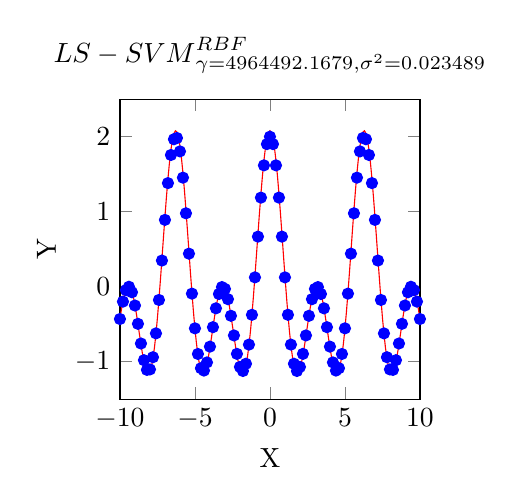
\begin{tikzpicture}

\begin{axis}[%
width=1.5in,
height=1.5in,
scale only axis,
xmin=-10,
xmax=10,
xlabel={X},
ymin=-1.5,
ymax=2.5,
ylabel={Y},
title={$\text{LS-SVM}_{\gamma\text{=4964492.1679,}\sigma{}^\text{2}\text{=0.023489}}^{\text{RBF}}$}
]
\addplot [color=red,solid,forget plot]
  table[row sep=crcr]{%
-10	-0.431331782639043\\
-9.9	-0.304119166472711\\
-9.8	-0.191764312900384\\
-9.7	-0.0999102841381132\\
-9.6	-0.0331842847589969\\
-9.5	0.00504946253817296\\
-9.4	0.012861876382152\\
-9.3	-0.0101466813382787\\
-9.2	-0.0628280477788594\\
-9.1	-0.142538739660447\\
-9	-0.245256401029012\\
-8.9	-0.365752546049465\\
-8.8	-0.497813526340048\\
-8.7	-0.634501184798639\\
-8.6	-0.768443863046565\\
-8.5	-0.892147308877627\\
-8.4	-0.998313805246278\\
-8.3	-1.08015685057651\\
-8.2	-1.13169829240203\\
-8.1	-1.14803517031083\\
-8	-1.12556471053985\\
-7.9	-1.06215782022146\\
-7.8	-0.957273832176739\\
-7.7	-0.81201189568464\\
-7.6	-0.629097078190218\\
-7.5	-0.412801800442894\\
-7.4	-0.168805619854606\\
-7.3	0.0960013950259457\\
-7.2	0.373764380798885\\
-7.1	0.6559492644935\\
-7	0.933657331029236\\
-6.9	1.19795656859519\\
-6.8	1.44021674017233\\
-6.7	1.65243485192024\\
-6.6	1.82753802941059\\
-6.5	1.959651753909\\
-6.4	2.04432287859189\\
-6.3	2.07868872880872\\
-6.2	2.06158577264405\\
-6.1	1.99359372214666\\
-6	1.87701340737194\\
-5.9	1.71577928799996\\
-5.8	1.51530996863337\\
-5.7	1.28230249290382\\
-5.6	1.0244784207661\\
-5.5	0.750291641419973\\
-5.4	0.468609437480446\\
-5.3	0.188379404656003\\
-5.2	-0.0817046153707543\\
-5.1	-0.333524436300959\\
-5	-0.559834660222095\\
-4.9	-0.754523491309057\\
-4.8	-0.912827171115857\\
-4.7	-1.03148983877496\\
-4.6	-1.10886278040785\\
-4.5	-1.14493941776539\\
-4.4	-1.14132491764175\\
-4.3	-1.10114189306176\\
-4.2	-1.02887621633861\\
-4.1	-0.930169366931768\\
-4	-0.811565887118153\\
-3.9	-0.680226318078802\\
-3.8	-0.543617358093292\\
-3.7	-0.409191867024891\\
-3.6	-0.284071707155647\\
-3.5	-0.174746254165592\\
-3.4	-0.0867987488032177\\
-3.3	-0.024671521266446\\
-3.2	0.00852044813269814\\
-3.1	0.0111201088895021\\
-3	-0.0170022205456315\\
-2.9	-0.0744433763276647\\
-2.8	-0.158326075992265\\
-2.7	-0.264419490065749\\
-2.6	-0.387316792045654\\
-2.5	-0.520662508569691\\
-2.4	-0.657420472644552\\
-2.3	-0.790171538601403\\
-2.2	-0.911429012075913\\
-2.1	-1.01395902648628\\
-2	-1.09109288440788\\
-1.9	-1.13701868417562\\
-1.8	-1.14704035686444\\
-1.7	-1.11779351634068\\
-1.6	-1.04740922739445\\
-1.5	-0.935618858970764\\
-1.4	-0.783795530564684\\
-1.3	-0.594930186503793\\
-1.2	-0.373542942908067\\
-1.1	-0.125532939456135\\
-1	0.142027612253058\\
-0.9	0.421147258913771\\
-0.799999999999999	0.703207171854714\\
-0.699999999999999	0.979279680268011\\
-0.6	1.24046102567082\\
-0.5	1.4782053078104\\
-0.399999999999999	1.68464652333176\\
-0.299999999999999	1.8528960480538\\
-0.199999999999999	1.97730386471602\\
-0.0999999999999996	2.05367325385993\\
0	2.07942049074634\\
0.0999999999999996	2.05367325385993\\
0.199999999999999	1.97730386471602\\
0.299999999999999	1.8528960480538\\
0.399999999999999	1.68464652333176\\
0.5	1.4782053078104\\
0.6	1.24046102567082\\
0.699999999999999	0.979279680268011\\
0.799999999999999	0.703207171854715\\
0.9	0.421147258913772\\
1	0.142027612253058\\
1.1	-0.125532939456135\\
1.2	-0.373542942908067\\
1.3	-0.594930186503793\\
1.4	-0.783795530564684\\
1.5	-0.935618858970764\\
1.6	-1.04740922739445\\
1.7	-1.11779351634068\\
1.8	-1.14704035686443\\
1.9	-1.13701868417562\\
2	-1.09109288440788\\
2.1	-1.01395902648628\\
2.2	-0.911429012075912\\
2.3	-0.790171538601403\\
2.4	-0.657420472644552\\
2.5	-0.520662508569692\\
2.6	-0.387316792045656\\
2.7	-0.264419490065749\\
2.8	-0.158326075992265\\
2.9	-0.0744433763276649\\
3	-0.017002220545631\\
3.1	0.0111201088895025\\
3.2	0.00852044813269881\\
3.3	-0.0246715212664457\\
3.4	-0.0867987488032185\\
3.5	-0.174746254165593\\
3.6	-0.284071707155648\\
3.7	-0.409191867024892\\
3.8	-0.543617358093293\\
3.9	-0.680226318078801\\
4	-0.811565887118153\\
4.1	-0.930169366931767\\
4.2	-1.02887621633861\\
4.3	-1.10114189306176\\
4.4	-1.14132491764175\\
4.5	-1.14493941776539\\
4.6	-1.10886278040785\\
4.7	-1.03148983877496\\
4.8	-0.912827171115855\\
4.9	-0.754523491309055\\
5	-0.559834660222093\\
5.1	-0.333524436300956\\
5.2	-0.0817046153707526\\
5.3	0.188379404656005\\
5.4	0.468609437480447\\
5.5	0.75029164141997\\
5.6	1.0244784207661\\
5.7	1.28230249290381\\
5.8	1.51530996863338\\
5.9	1.71577928799997\\
6	1.87701340737195\\
6.1	1.99359372214667\\
6.2	2.06158577264406\\
6.3	2.07868872880873\\
6.4	2.04432287859189\\
6.5	1.959651753909\\
6.6	1.82753802941059\\
6.7	1.65243485192024\\
6.8	1.44021674017233\\
6.9	1.19795656859519\\
7	0.933657331029237\\
7.1	0.6559492644935\\
7.2	0.37376438079889\\
7.3	0.0960013950259471\\
7.4	-0.16880561985461\\
7.5	-0.412801800442904\\
7.6	-0.629097078190218\\
7.7	-0.812011895684628\\
7.8	-0.957273832176735\\
7.9	-1.06215782022144\\
8	-1.12556471053984\\
8.1	-1.14803517031082\\
8.2	-1.13169829240202\\
8.3	-1.08015685057649\\
8.4	-0.998313805246246\\
8.5	-0.89214730887763\\
8.6	-0.768443863046565\\
8.7	-0.634501184798624\\
8.8	-0.497813526340026\\
8.9	-0.365752546049458\\
9	-0.245256401028998\\
9.1	-0.142538739660397\\
9.2	-0.0628280477788452\\
9.3	-0.010146681338236\\
9.4	0.012861876382152\\
9.5	0.00504946253817296\\
9.6	-0.0331842847589685\\
9.7	-0.099910284138099\\
9.8	-0.191764312900369\\
9.9	-0.304119166472697\\
10	-0.431331782639015\\
};
\addplot [color=blue,only marks,mark=*,mark options={solid},forget plot]
  table[row sep=crcr]{%
-10	-0.43098946726306\\
-9.8	-0.199040176459257\\
-9.6	-0.0454675090972562\\
-9.4	-0.000920685447996283\\
-9.2	-0.0742034490193951\\
-9	-0.250813553640597\\
-8.8	-0.495349259142413\\
-8.6	-0.757398242051853\\
-8.4	-0.979967241528048\\
-8.2	-1.10910282152591\\
-8	-1.103159514132\\
-7.8	-0.940222204621165\\
-7.6	-0.622477140428825\\
-7.4	-0.17680515538033\\
-7.2	0.348533958318501\\
-7	0.890639472551138\\
-6.8	1.38110148280297\\
-6.6	1.75611654959898\\
-6.4	1.96601748445563\\
-6.2	1.98273439930208\\
-6	1.80402424538286\\
-5.8	1.45380914670929\\
-5.6	0.978570742329\\
-5.4	0.440362969487297\\
-5.2	-0.0924675861268539\\
-5	-0.555409343613226\\
-4.8	-0.897188872354681\\
-4.6	-1.08699614833922\\
-4.4	-1.11842588404008\\
-4.2	-1.00954947545738\\
-4	-0.799143654672225\\
-3.8	-0.539707869332161\\
-3.6	-0.288407101801892\\
-3.4	-0.0974007022296354\\
-3.2	-0.00510985703656031\\
-3	-0.0298222099500793\\
-2.8	-0.166656462158408\\
-2.6	-0.388372082068571\\
-2.4	-0.6498947321018\\
-2.2	-0.895833987233766\\
-2	-1.06979045741075\\
-1.8	-1.12396051102723\\
-1.6	-1.02749429809604\\
-1.4	-0.772255197768418\\
-1.2	-0.37503596106457\\
-1	0.124155469320997\\
-0.799999999999999	0.66750718704588\\
-0.6	1.18769336938635\\
-0.399999999999999	1.61776770335005\\
-0.199999999999999	1.90112757184413\\
0	2\\
0.199999999999999	1.90112757184413\\
0.399999999999999	1.61776770335005\\
0.6	1.18769336938635\\
0.799999999999999	0.66750718704588\\
1	0.124155469320997\\
1.2	-0.37503596106457\\
1.4	-0.772255197768418\\
1.6	-1.02749429809604\\
1.8	-1.12396051102723\\
2	-1.06979045741075\\
2.2	-0.895833987233766\\
2.4	-0.6498947321018\\
2.6	-0.388372082068571\\
2.8	-0.166656462158408\\
3	-0.0298222099500793\\
3.2	-0.00510985703656031\\
3.4	-0.0974007022296354\\
3.6	-0.288407101801892\\
3.8	-0.539707869332161\\
4	-0.799143654672225\\
4.2	-1.00954947545738\\
4.4	-1.11842588404008\\
4.6	-1.08699614833922\\
4.8	-0.897188872354681\\
5	-0.555409343613226\\
5.2	-0.0924675861268539\\
5.4	0.440362969487297\\
5.6	0.978570742329\\
5.8	1.45380914670929\\
6	1.80402424538286\\
6.2	1.98273439930208\\
6.4	1.96601748445563\\
6.6	1.75611654959898\\
6.8	1.38110148280297\\
7	0.890639472551138\\
7.2	0.348533958318501\\
7.4	-0.17680515538033\\
7.6	-0.622477140428825\\
7.8	-0.940222204621165\\
8	-1.103159514132\\
8.2	-1.10910282152591\\
8.4	-0.979967241528048\\
8.6	-0.757398242051853\\
8.8	-0.495349259142413\\
9	-0.250813553640597\\
9.2	-0.0742034490193951\\
9.4	-0.000920685447996283\\
9.6	-0.0454675090972562\\
9.8	-0.199040176459257\\
10	-0.43098946726306\\
};
\end{axis}
\end{tikzpicture}%
\end{document}
% This file was created by matlab2tikz.
% Minimal pgfplots version: 1.3
%
%The latest updates can be retrieved from
%  http://www.mathworks.com/matlabcentral/fileexchange/22022-matlab2tikz
%where you can also make suggestions and rate matlab2tikz.
%
\documentclass[tikz]{standalone}
\usepackage{pgfplots}
\usepackage{grffile}
\pgfplotsset{compat=newest}
\usetikzlibrary{plotmarks}
\usepackage{amsmath}

\begin{document}
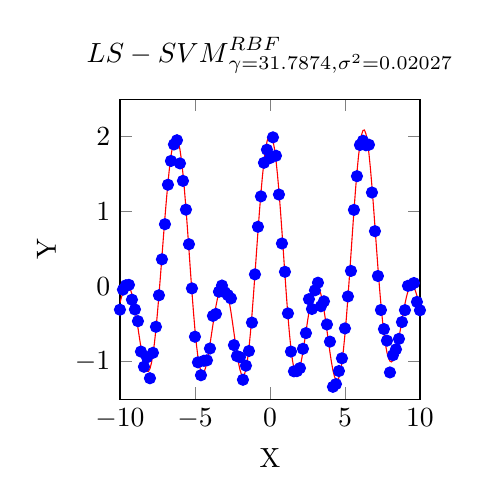
\begin{tikzpicture}

\begin{axis}[%
width=1.5in,
height=1.5in,
scale only axis,
xmin=-10,
xmax=10,
xlabel={X},
ymin=-1.5,
ymax=2.5,
ylabel={Y},
title={$\text{LS-SVM}_{\gamma\text{=31.7874,}\sigma{}^\text{2}\text{=0.02027}}^{\text{RBF}}$}
]
\addplot [color=red,solid,forget plot]
  table[row sep=crcr]{%
-10	-0.213262761564271\\
-9.9	-0.142478591462586\\
-9.8	-0.0793448278600375\\
-9.7	-0.0290871299652287\\
-9.6	0.00354128627906709\\
-9.5	0.0146389231847516\\
-9.4	0.0014854442796632\\
-9.3	-0.0372068057317912\\
-9.2	-0.101139578126474\\
-9.1	-0.188384754784025\\
-9	-0.295450732940575\\
-8.9	-0.417451111552073\\
-8.8	-0.54836015761066\\
-8.7	-0.681334313311297\\
-8.6	-0.809076237391692\\
-8.5	-0.924217391705701\\
-8.4	-1.01969655619064\\
-8.3	-1.0891143088334\\
-8.2	-1.12704685556991\\
-8.1	-1.12930614622694\\
-8	-1.0931366396388\\
-7.9	-1.01734224738166\\
-7.8	-0.902339926115156\\
-7.7	-0.750139254299917\\
-7.6	-0.564250307417169\\
-7.5	-0.349525371771638\\
-7.4	-0.111943512746484\\
-7.3	0.141649446458759\\
-7.2	0.403829761333681\\
-7.1	0.666895294241502\\
-7	0.923156741856179\\
-6.9	1.16520271391615\\
-6.8	1.38612426199147\\
-6.7	1.57969009939048\\
-6.6	1.74047099768306\\
-6.5	1.86391961687912\\
-6.4	1.94641889960253\\
-6.3	1.98531660850333\\
-6.2	1.97896431730091\\
-6.1	1.92677546758146\\
-6	1.82930912405298\\
-5.9	1.68837493150389\\
-5.8	1.50714251968933\\
-5.7	1.29022781256321\\
-5.6	1.04372203972044\\
-5.5	0.775128863897808\\
-5.4	0.493182006037289\\
-5.3	0.207529715069586\\
-5.2	-0.071708469581301\\
-5.1	-0.334486097297755\\
-5	-0.571429448456664\\
-4.9	-0.774432825918838\\
-4.8	-0.937184670987546\\
-4.7	-1.0555644603051\\
-4.6	-1.12786474973692\\
-4.5	-1.15481458840091\\
-4.4	-1.1394062281282\\
-4.3	-1.08655226706847\\
-4.2	-1.00262086443906\\
-4.1	-0.894909135000068\\
-4	-0.771117488512349\\
-3.9	-0.638880545664861\\
-3.8	-0.505395098113482\\
-3.7	-0.377165472976204\\
-3.6	-0.25986538284936\\
-3.5	-0.15829661720152\\
-3.4	-0.076411771861751\\
-3.3	-0.0173624363293186\\
-3.2	0.0164637355722698\\
-3.1	0.0234448149594588\\
-3	0.00277935713259821\\
-2.9	-0.0454075474076457\\
-2.8	-0.119923772719122\\
-2.7	-0.2183641248049\\
-2.6	-0.336994853900915\\
-2.5	-0.470706035278767\\
-2.4	-0.613064335527356\\
-2.3	-0.756488469166245\\
-2.2	-0.892555322646579\\
-2.1	-1.01242803698707\\
-2	-1.10738034141795\\
-1.9	-1.16937626873803\\
-1.8	-1.19165312213254\\
-1.7	-1.16924996613922\\
-1.6	-1.09942520913916\\
-1.5	-0.981915488238706\\
-1.4	-0.819003554392686\\
-1.3	-0.615383630150048\\
-1.2	-0.377836240340386\\
-1.1	-0.114747552622217\\
-1	0.164472689812005\\
-0.9	0.450008676734924\\
-0.799999999999999	0.732223019284894\\
-0.699999999999999	1.00214743291159\\
-0.6	1.25183573335143\\
-0.5	1.4745587727785\\
-0.399999999999999	1.66484713941422\\
-0.299999999999999	1.81841179086765\\
-0.199999999999999	1.9319909725078\\
-0.0999999999999996	2.00318052340469\\
0	2.03030243327841\\
0.0999999999999996	2.01235375272024\\
0.199999999999999	1.9490571002878\\
0.299999999999999	1.84100897769933\\
0.399999999999999	1.68989757532998\\
0.5	1.49874227573526\\
0.6	1.27209623402352\\
0.699999999999999	1.01615323295254\\
0.799999999999999	0.738710578626992\\
0.9	0.448959362048358\\
1	0.157098712729086\\
1.1	-0.126202428525651\\
1.2	-0.39044831118337\\
1.3	-0.625998791179181\\
1.4	-0.824717390134193\\
1.5	-0.980513307168073\\
1.6	-1.08971791571495\\
1.7	-1.1512567825635\\
1.8	-1.16660396654407\\
1.9	-1.13953247696962\\
2	-1.07569929730269\\
2.1	-0.982121710256422\\
2.2	-0.866611146612672\\
2.3	-0.737230143216886\\
2.4	-0.601827564140509\\
2.5	-0.467688940360609\\
2.6	-0.341315873120573\\
2.7	-0.228324993343533\\
2.8	-0.133437165178842\\
2.9	-0.060515022395779\\
3	-0.0126037695411765\\
3.1	0.00806308650816608\\
3.2	0.000116272064347903\\
3.3	-0.0368356050941697\\
3.4	-0.102049718523326\\
3.5	-0.193486050118584\\
3.6	-0.307683942198122\\
3.7	-0.439724546268655\\
3.8	-0.583315519240117\\
3.9	-0.731015883150585\\
4	-0.874595734026874\\
4.1	-1.00550212743108\\
4.2	-1.11538370966229\\
4.3	-1.19661627704551\\
4.4	-1.2427714403565\\
4.5	-1.24898077212411\\
4.6	-1.2121659244801\\
4.7	-1.13112733482442\\
4.8	-1.00650567509119\\
4.9	-0.840646828572783\\
5	-0.637409792058949\\
5.1	-0.401956242950502\\
5.2	-0.140551377926988\\
5.3	0.139609372295335\\
5.4	0.430550229711158\\
5.5	0.723659079426593\\
5.6	1.00985257446882\\
5.7	1.27979089273586\\
5.8	1.52416389161494\\
5.9	1.73405645184522\\
6	1.90138246596415\\
6.1	2.01935789597182\\
6.2	2.0829674870494\\
6.3	2.08937042591654\\
6.4	2.03818966147804\\
6.5	1.93163839679352\\
6.6	1.77445438508569\\
6.7	1.57363560131742\\
6.8	1.33799604082844\\
6.9	1.07758379403096\\
7	0.803021370673836\\
7.1	0.52483758664266\\
7.2	0.252859647769602\\
7.3	-0.00427651495553931\\
7.4	-0.239458330216288\\
7.5	-0.447255531456874\\
7.6	-0.623915292766853\\
7.7	-0.76722483255608\\
7.8	-0.876288257145369\\
7.9	-0.951271114914958\\
8	-0.993163247560142\\
8.1	-1.00359895046241\\
8.2	-0.984755579630112\\
8.3	-0.939331013226149\\
8.4	-0.870580666246955\\
8.5	-0.782379680020918\\
8.6	-0.679268179278144\\
8.7	-0.56643846074942\\
8.8	-0.449632419326794\\
8.9	-0.334933684198312\\
9	-0.228458894122546\\
9.1	-0.135972700243537\\
9.2	-0.0624678446152139\\
9.3	-0.0117620385539706\\
9.4	0.013834497549275\\
9.5	0.0137334936510258\\
9.6	-0.010868124858183\\
9.7	-0.0570900080219115\\
9.8	-0.120627416327316\\
9.9	-0.196139480243158\\
10	-0.277722702248705\\
};
\addplot [color=blue,only marks,mark=*,mark options={solid},forget plot]
  table[row sep=crcr]{%
-10	-0.306579133527982\\
-9.8	-0.0397382555553657\\
-9.6	0.018739660609576\\
-9.4	0.0242905480075732\\
-9.2	-0.173380769716921\\
-9	-0.303452947386662\\
-8.8	-0.459547263627656\\
-8.6	-0.865085860768563\\
-8.4	-1.06784448545167\\
-8.2	-0.941742958419704\\
-8	-1.22066061822186\\
-7.8	-0.881877827486431\\
-7.6	-0.534964538044644\\
-7.4	-0.114653722995193\\
-7.2	0.365063866304641\\
-7	0.833183768477336\\
-6.8	1.3593888028889\\
-6.6	1.6764672224338\\
-6.4	1.89657728080095\\
-6.2	1.95242004354036\\
-6	1.64392823759623\\
-5.8	1.41069727246189\\
-5.6	1.02715004301935\\
-5.4	0.566008817029371\\
-5.2	-0.0226588916021791\\
-5	-0.667002890632711\\
-4.8	-1.00885127695319\\
-4.6	-1.18052735154478\\
-4.4	-0.987745467811725\\
-4.2	-0.982006760185838\\
-4	-0.82409491495306\\
-3.8	-0.389406083461653\\
-3.6	-0.362798054582325\\
-3.4	-0.0668089334738737\\
-3.2	0.0152031165919985\\
-3	-0.0756469343852673\\
-2.8	-0.112338464968575\\
-2.6	-0.156181529203947\\
-2.4	-0.77899329546166\\
-2.2	-0.924930542321883\\
-2	-0.939996483241433\\
-1.8	-1.24123176786791\\
-1.6	-1.05325139523663\\
-1.4	-0.857442817230265\\
-1.2	-0.47867949734374\\
-1	0.164137461033253\\
-0.799999999999999	0.798528324906496\\
-0.6	1.20425025884851\\
-0.399999999999999	1.65189112389713\\
-0.199999999999999	1.82666452394961\\
0	1.71497122229152\\
0.199999999999999	1.99125121667456\\
0.399999999999999	1.74601395259658\\
0.6	1.22859304817884\\
0.799999999999999	0.576006043167302\\
1	0.198369702065894\\
1.2	-0.356093645541498\\
1.4	-0.864817391491114\\
1.6	-1.12859035792103\\
1.8	-1.12571135333162\\
2	-1.08541915281891\\
2.2	-0.828146555519386\\
2.4	-0.619062350438906\\
2.6	-0.166384116930707\\
2.8	-0.297194787264751\\
3	-0.0483218061484544\\
3.2	0.053009933786154\\
3.4	-0.260413518102873\\
3.6	-0.195231272475295\\
3.8	-0.503916733277877\\
4	-0.732599750127662\\
4.2	-1.33524884529104\\
4.4	-1.2985987129247\\
4.6	-1.12472571614096\\
4.8	-0.954881987385641\\
5	-0.556407122309299\\
5.2	-0.130055763458628\\
5.4	0.209937041851235\\
5.6	1.02393741156959\\
5.8	1.47338319728387\\
6	1.88951982345171\\
6.2	1.94540993806249\\
6.4	1.88609300482996\\
6.6	1.89243215815344\\
6.8	1.25572426230034\\
7	0.740131583568841\\
7.2	0.14248777755351\\
7.4	-0.310578825334796\\
7.6	-0.565333766918074\\
7.8	-0.719470674351168\\
8	-1.14341280005323\\
8.2	-0.913369219359977\\
8.4	-0.835654817371107\\
8.6	-0.695767150416593\\
8.8	-0.471530820082818\\
9	-0.31262727143036\\
9.2	0.0114268286448022\\
9.4	0.0205720531660902\\
9.6	0.0490609089602083\\
9.8	-0.20311160964176\\
10	-0.314123795052465\\
};
\end{axis}
\end{tikzpicture}%
\end{document}
\caption{Exemplary tuning results on noise free and noisy data.}
\label{fig:autoTune}
\end{figure}
\begin{figure}
\centering
% This file was created by matlab2tikz.
% Minimal pgfplots version: 1.3
%
%The latest updates can be retrieved from
%  http://www.mathworks.com/matlabcentral/fileexchange/22022-matlab2tikz
%where you can also make suggestions and rate matlab2tikz.
%
\documentclass[tikz]{standalone}
\usepackage{pgfplots}
\usepackage{grffile}
\pgfplotsset{compat=newest}
\usetikzlibrary{plotmarks}
\usepackage{amsmath}

\begin{document}
\begin{tikzpicture}

\begin{axis}[%
width=2.5in,
height=2.5in,
at={(0.758333in,0.48125in)},
scale only axis,
xmin=-6,
xmax=0,
tick align=outside,
xlabel={$\sigma^2$},
xmajorgrids,
ymin=0,
ymax=10,
ylabel={$\gamma$},
ymajorgrids,
zmin=0,
zmax=1,
zlabel={$\log_{10}(\| \mathbf{y}_{\text{est}} - \mathbf{y}\|_2)$},
zmajorgrids,
view={84.4}{22},
axis x line*=bottom,
axis y line*=left,
axis z line*=left
]

\addplot3[%
surf,
shader=flat,
colormap={mymap}{[1pt] rgb(0pt)=(0.2081,0.1663,0.5292); rgb(1pt)=(0.211624,0.189781,0.577676); rgb(2pt)=(0.212252,0.213771,0.626971); rgb(3pt)=(0.2081,0.2386,0.677086); rgb(4pt)=(0.195905,0.264457,0.7279); rgb(5pt)=(0.170729,0.291938,0.779248); rgb(6pt)=(0.125271,0.324243,0.830271); rgb(7pt)=(0.0591333,0.359833,0.868333); rgb(8pt)=(0.0116952,0.38751,0.881957); rgb(9pt)=(0.00595714,0.408614,0.882843); rgb(10pt)=(0.0165143,0.4266,0.878633); rgb(11pt)=(0.0328524,0.443043,0.871957); rgb(12pt)=(0.0498143,0.458571,0.864057); rgb(13pt)=(0.0629333,0.47369,0.855438); rgb(14pt)=(0.0722667,0.488667,0.8467); rgb(15pt)=(0.0779429,0.503986,0.838371); rgb(16pt)=(0.0793476,0.520024,0.831181); rgb(17pt)=(0.0749429,0.537543,0.826271); rgb(18pt)=(0.0640571,0.556986,0.823957); rgb(19pt)=(0.0487714,0.577224,0.822829); rgb(20pt)=(0.0343429,0.596581,0.819852); rgb(21pt)=(0.0265,0.6137,0.8135); rgb(22pt)=(0.0238905,0.628662,0.803762); rgb(23pt)=(0.0230905,0.641786,0.791267); rgb(24pt)=(0.0227714,0.653486,0.776757); rgb(25pt)=(0.0266619,0.664195,0.760719); rgb(26pt)=(0.0383714,0.674271,0.743552); rgb(27pt)=(0.0589714,0.683757,0.725386); rgb(28pt)=(0.0843,0.692833,0.706167); rgb(29pt)=(0.113295,0.7015,0.685857); rgb(30pt)=(0.145271,0.709757,0.664629); rgb(31pt)=(0.180133,0.717657,0.642433); rgb(32pt)=(0.217829,0.725043,0.619262); rgb(33pt)=(0.258643,0.731714,0.595429); rgb(34pt)=(0.302171,0.737605,0.571186); rgb(35pt)=(0.348167,0.742433,0.547267); rgb(36pt)=(0.395257,0.7459,0.524443); rgb(37pt)=(0.44201,0.748081,0.503314); rgb(38pt)=(0.487124,0.749062,0.483976); rgb(39pt)=(0.530029,0.749114,0.466114); rgb(40pt)=(0.570857,0.748519,0.44939); rgb(41pt)=(0.609852,0.747314,0.433686); rgb(42pt)=(0.6473,0.7456,0.4188); rgb(43pt)=(0.683419,0.743476,0.404433); rgb(44pt)=(0.71841,0.741133,0.390476); rgb(45pt)=(0.752486,0.7384,0.376814); rgb(46pt)=(0.785843,0.735567,0.363271); rgb(47pt)=(0.818505,0.732733,0.34979); rgb(48pt)=(0.850657,0.7299,0.336029); rgb(49pt)=(0.882433,0.727433,0.3217); rgb(50pt)=(0.913933,0.725786,0.306276); rgb(51pt)=(0.944957,0.726114,0.288643); rgb(52pt)=(0.973895,0.731395,0.266648); rgb(53pt)=(0.993771,0.745457,0.240348); rgb(54pt)=(0.999043,0.765314,0.216414); rgb(55pt)=(0.995533,0.786057,0.196652); rgb(56pt)=(0.988,0.8066,0.179367); rgb(57pt)=(0.978857,0.827143,0.163314); rgb(58pt)=(0.9697,0.848138,0.147452); rgb(59pt)=(0.962586,0.870514,0.1309); rgb(60pt)=(0.958871,0.8949,0.113243); rgb(61pt)=(0.959824,0.921833,0.0948381); rgb(62pt)=(0.9661,0.951443,0.0755333); rgb(63pt)=(0.9763,0.9831,0.0538)},
mesh/rows=100]
table[row sep=crcr,header=false] {%
%
-5	0	0.986800874304542\\
-5	0.101010101010101	0.986800052280902\\
-5	0.202020202020202	0.986796807052418\\
-5	0.303030303030303	0.986785906604203\\
-5	0.404040404040404	0.986754208645049\\
-5	0.505050505050505	0.98667315578271\\
-5	0.606060606060606	0.986488347073383\\
-5	0.707070707070707	0.986107850683925\\
-5	0.808080808080808	0.985392404237292\\
-5	0.909090909090909	0.984151149414813\\
-5	1.01010101010101	0.982145527937436\\
-5	1.11111111111111	0.979101724610159\\
-5	1.21212121212121	0.974729572885481\\
-5	1.31313131313131	0.968744212729524\\
-5	1.41414141414141	0.960886569581003\\
-5	1.51515151515152	0.950939793693995\\
-5	1.61616161616162	0.938740634600965\\
-5	1.71717171717172	0.924186731221776\\
-5	1.81818181818182	0.907242453304208\\
-5	1.91919191919192	0.88794672455495\\
-5	2.02020202020202	0.866425638597369\\
-5	2.12121212121212	0.842910185689902\\
-5	2.22222222222222	0.81775503756759\\
-5	2.32323232323232	0.791449057449495\\
-5	2.42424242424242	0.764604384389564\\
-5	2.52525252525253	0.737912129155553\\
-5	2.62626262626263	0.712061887247271\\
-5	2.72727272727273	0.687638527046106\\
-5	2.82828282828283	0.665025754590351\\
-5	2.92929292929293	0.644350616387468\\
-5	3.03030303030303	0.625489920641417\\
-5	3.13131313131313	0.608134325696348\\
-5	3.23232323232323	0.591883581547694\\
-5	3.33333333333333	0.576339286929769\\
-5	3.43434343434343	0.561170245366577\\
-5	3.53535353535354	0.546141679489212\\
-5	3.63636363636364	0.531113795639187\\
-5	3.73737373737374	0.516022448505581\\
-5	3.83838383838384	0.500854760352128\\
-5	3.93939393939394	0.485628237966321\\
-5	4.04040404040404	0.470376656260544\\
-5	4.14141414141414	0.455142215651635\\
-5	4.24242424242424	0.439971963820439\\
-5	4.34343434343434	0.424916566440049\\
-5	4.44444444444444	0.410030204310455\\
-5	4.54545454545455	0.395370997476369\\
-5	4.64646464646465	0.381001686497439\\
-5	4.74747474747475	0.366990374495007\\
-5	4.84848484848485	0.353411126617762\\
-5	4.94949494949495	0.340344339328778\\
-5	5.05050505050505	0.327877058095626\\
-5	5.15151515151515	0.316103606289724\\
-5	5.25252525252525	0.305126737900444\\
-5	5.35353535353535	0.295059106615593\\
-5	5.45454545454545	0.286024599876107\\
-5	5.55555555555556	0.278159519534329\\
-5	5.65656565656566	0.271614665337623\\
-5	5.75757575757576	0.26656020708222\\
-5	5.85858585858586	0.263194709227678\\
-5	5.95959595959596	0.261757637412619\\
-5	6.06060606060606	0.262542277469973\\
-5	6.16161616161616	0.265904849683473\\
-5	6.26262626262626	0.272266457446586\\
-5	6.36363636363636	0.282106235212402\\
-5	6.46464646464646	0.295944255262722\\
-5	6.56565656565657	0.31431039750217\\
-5	6.66666666666667	0.337692621072666\\
-5	6.76767676767677	0.366458705381339\\
-5	6.86868686868687	0.400751808571746\\
-5	6.96969696969697	0.440370900329395\\
-5	7.07070707070707	0.484658560283926\\
-5	7.17171717171717	0.532427878812743\\
-5	7.27272727272727	0.58196674806905\\
-5	7.37373737373737	0.631158098522961\\
-5	7.47474747474747	0.677734917297178\\
-5	7.57575757575758	0.719637713513337\\
-5	7.67676767676768	0.755381563082472\\
-5	7.77777777777778	0.784319030793969\\
-5	7.87878787878788	0.806717806794324\\
-5	7.97979797979798	0.823626645915746\\
-5	8.08080808080808	0.836569481028359\\
-5	8.18181818181818	0.847184372259599\\
-5	8.28282828282828	0.856946344056499\\
-5	8.38383838383838	0.867019330269337\\
-5	8.48484848484848	0.878163312159207\\
-5	8.58585858585859	0.890640133719253\\
-5	8.68686868686869	0.904186476632672\\
-5	8.78787878787879	0.918146056890494\\
-5	8.88888888888889	0.931717144134434\\
-5	8.98989898989899	0.944171761646631\\
-5	9.09090909090909	0.954967203587162\\
-5	9.19191919191919	0.963781869964616\\
-5	9.29292929292929	0.970528011902406\\
-5	9.39393939393939	0.975344853319058\\
-5	9.49494949494949	0.978549813320997\\
-5	9.5959595959596	0.980550727566435\\
-5	9.6969696969697	0.981752751150766\\
-5	9.7979797979798	0.98249264847716\\
-5	9.8989898989899	0.983010361504468\\
-5	10	0.983449607478337\\
-4.94949494949495	0	0.986800850184986\\
-4.94949494949495	0.101010101010101	0.986799932994897\\
-4.94949494949495	0.202020202020202	0.986796312061342\\
-4.94949494949495	0.303030303030303	0.986784149629036\\
-4.94949494949495	0.404040404040404	0.986748781686026\\
-4.94949494949495	0.505050505050505	0.986658343203955\\
-4.94949494949495	0.606060606060606	0.986452127158481\\
-4.94949494949495	0.707070707070707	0.986027524499241\\
-4.94949494949495	0.808080808080808	0.985229030438281\\
-4.94949494949495	0.909090909090909	0.983843337186886\\
-4.94949494949495	1.01010101010101	0.981603374051074\\
-4.94949494949495	1.11111111111111	0.978201652483248\\
-4.94949494949495	1.21212121212121	0.973310549415495\\
-4.94949494949495	1.31313131313131	0.966605411855315\\
-4.94949494949495	1.41414141414141	0.957786193102856\\
-4.94949494949495	1.51515151515152	0.946594588891576\\
-4.94949494949495	1.61616161616162	0.932825745091541\\
-4.94949494949495	1.71717171717172	0.916335924058888\\
-4.94949494949495	1.81818181818182	0.897049498227987\\
-4.94949494949495	1.91919191919192	0.874969717742831\\
-4.94949494949495	2.02020202020202	0.850197176007501\\
-4.94949494949495	2.12121212121212	0.822957062892214\\
-4.94949494949495	2.22222222222222	0.793630828328843\\
-4.94949494949495	2.32323232323232	0.762780528367546\\
-4.94949494949495	2.42424242424242	0.731147549615855\\
-4.94949494949495	2.52525252525253	0.699606504579967\\
-4.94949494949495	2.62626262626263	0.669065332761623\\
-4.94949494949495	2.72727272727273	0.640325214936396\\
-4.94949494949495	2.82828282828283	0.61393998447099\\
-4.94949494949495	2.92929292929293	0.590126517204062\\
-4.94949494949495	3.03030303030303	0.56876158720061\\
-4.94949494949495	3.13131313131313	0.549463116964059\\
-4.94949494949495	3.23232323232323	0.531718623612753\\
-4.94949494949495	3.33333333333333	0.515011892899401\\
-4.94949494949495	3.43434343434343	0.498911969592776\\
-4.94949494949495	3.53535353535354	0.483112540375897\\
-4.94949494949495	3.63636363636364	0.467429973371728\\
-4.94949494949495	3.73737373737374	0.451777786722092\\
-4.94949494949495	3.83838383838384	0.436134793037321\\
-4.94949494949495	3.93939393939394	0.420517978226654\\
-4.94949494949495	4.04040404040404	0.404964116631046\\
-4.94949494949495	4.14141414141414	0.389519337916516\\
-4.94949494949495	4.24242424242424	0.374234071601577\\
-4.94949494949495	4.34343434343434	0.359161001611087\\
-4.94949494949495	4.44444444444444	0.344354535057012\\
-4.94949494949495	4.54545454545455	0.329871051421791\\
-4.94949494949495	4.64646464646465	0.315769604270631\\
-4.94949494949495	4.74747474747475	0.302112784814028\\
-4.94949494949495	4.84848484848485	0.288967332613201\\
-4.94949494949495	4.94949494949495	0.276404202192675\\
-4.94949494949495	5.05050505050505	0.264498335912946\\
-4.94949494949495	5.15151515151515	0.253328906796124\\
-4.94949494949495	5.25252525252525	0.242980631574055\\
-4.94949494949495	5.35353535353535	0.233545857363025\\
-4.94949494949495	5.45454545454545	0.225126273997565\\
-4.94949494949495	5.55555555555556	0.217833441583294\\
-4.94949494949495	5.65656565656566	0.211789283043184\\
-4.94949494949495	5.75757575757576	0.207129939795461\\
-4.94949494949495	5.85858585858586	0.204016504556723\\
-4.94949494949495	5.95959595959596	0.202653114983473\\
-4.94949494949495	6.06060606060606	0.203308440203375\\
-4.94949494949495	6.16161616161616	0.206333836235913\\
-4.94949494949495	6.26262626262626	0.212172564132419\\
-4.94949494949495	6.36363636363636	0.221358413290844\\
-4.94949494949495	6.46464646464646	0.234504191615882\\
-4.94949494949495	6.56565656565657	0.252277058228965\\
-4.94949494949495	6.66666666666667	0.275350854205585\\
-4.94949494949495	6.76767676767677	0.30432252928839\\
-4.94949494949495	6.86868686868687	0.339586442860231\\
-4.94949494949495	6.96969696969697	0.381176585624139\\
-4.94949494949495	7.07070707070707	0.428605709122066\\
-4.94949494949495	7.17171717171717	0.480743389877499\\
-4.94949494949495	7.27272727272727	0.535780445389686\\
-4.94949494949495	7.37373737373737	0.591328379993751\\
-4.94949494949495	7.47474747474747	0.644689558181273\\
-4.94949494949495	7.57575757575758	0.693280027876764\\
-4.94949494949495	7.67676767676768	0.735099319425392\\
-4.94949494949495	7.77777777777778	0.769094110149413\\
-4.94949494949495	7.87878787878788	0.795303915022012\\
-4.94949494949495	7.97979797979798	0.814753099301453\\
-4.94949494949495	8.08080808080808	0.829119341579815\\
-4.94949494949495	8.18181818181818	0.840294371330776\\
-4.94949494949495	8.28282828282828	0.850021547390767\\
-4.94949494949495	8.38383838383838	0.859718962393778\\
-4.94949494949495	8.48484848484848	0.870406953135935\\
-4.94949494949495	8.58585858585859	0.882602882730344\\
-4.94949494949495	8.68686868686869	0.896218316120991\\
-4.94949494949495	8.78787878787879	0.910628687347231\\
-4.94949494949495	8.88888888888889	0.924949716419923\\
-4.94949494949495	8.98989898989899	0.938340670398327\\
-4.94949494949495	9.09090909090909	0.950166504175221\\
-4.94949494949495	9.19191919191919	0.960027382308248\\
-4.94949494949495	9.29292929292929	0.96775285966402\\
-4.94949494949495	9.39393939393939	0.973402466642345\\
-4.94949494949495	9.49494949494949	0.977242592979172\\
-4.94949494949495	9.5959595959596	0.979673828882945\\
-4.94949494949495	9.6969696969697	0.981130981822487\\
-4.94949494949495	9.7979797979798	0.981998936065606\\
-4.94949494949495	9.8989898989899	0.982567825571696\\
-4.94949494949495	10	0.983023992457035\\
-4.8989898989899	0	0.986800826703419\\
-4.8989898989899	0.101010101010101	0.986799816864121\\
-4.8989898989899	0.202020202020202	0.98679583016285\\
-4.8989898989899	0.303030303030303	0.986782439121292\\
-4.8989898989899	0.404040404040404	0.986743498212708\\
-4.8989898989899	0.505050505050505	0.986643921959463\\
-4.8989898989899	0.606060606060606	0.986416862455625\\
-4.8989898989899	0.707070707070707	0.985949309028022\\
-4.8989898989899	0.808080808080808	0.985069920106504\\
-4.8989898989899	0.909090909090909	0.983543461148873\\
-4.8989898989899	1.01010101010101	0.981074922098604\\
-4.8989898989899	1.11111111111111	0.977323627149208\\
-4.8989898989899	1.21212121212121	0.971924680303621\\
-4.8989898989899	1.31313131313131	0.964513224620711\\
-4.8989898989899	1.41414141414141	0.954746874027163\\
-4.8989898989899	1.51515151515152	0.942323122053313\\
-4.8989898989899	1.61616161616162	0.926990903998178\\
-4.8989898989899	1.71717171717172	0.90855812976553\\
-4.8989898989899	1.81818181818182	0.886899363456005\\
-4.8989898989899	1.91919191919192	0.86196929693933\\
-4.8989898989899	2.02020202020202	0.83382741860485\\
-4.8989898989899	2.12121212121212	0.802676324080292\\
-4.8989898989899	2.22222222222222	0.768909674053349\\
-4.8989898989899	2.32323232323232	0.733156092640995\\
-4.8989898989899	2.42424242424242	0.696294840556944\\
-4.8989898989899	2.52525252525253	0.659414063385581\\
-4.8989898989899	2.62626262626263	0.623691878607656\\
-4.8989898989899	2.72727272727273	0.590210277856518\\
-4.8989898989899	2.82828282828283	0.559753080857388\\
-4.8989898989899	2.92929292929293	0.532664732216443\\
-4.8989898989899	3.03030303030303	0.508829439176377\\
-4.8989898989899	3.13131313131313	0.487774062961253\\
-4.8989898989899	3.23232323232323	0.468842022577971\\
-4.8989898989899	3.33333333333333	0.45136614261303\\
-4.8989898989899	3.43434343434343	0.434788699879071\\
-4.8989898989899	3.53535353535354	0.418713093928141\\
-4.8989898989899	3.63636363636364	0.402900163836819\\
-4.8989898989899	3.73737373737374	0.38723416956749\\
-4.8989898989899	3.83838383838384	0.37168144678023\\
-4.8989898989899	3.93939393939394	0.356255724785729\\
-4.8989898989899	4.04040404040404	0.34099467689105\\
-4.8989898989899	4.14141414141414	0.325946335523223\\
-4.8989898989899	4.24242424242424	0.311162095333656\\
-4.8989898989899	4.34343434343434	0.296693503481518\\
-4.8989898989899	4.44444444444444	0.282591106698022\\
-4.8989898989899	4.54545454545455	0.268904489570452\\
-4.8989898989899	4.64646464646465	0.255683138282566\\
-4.8989898989899	4.74747474747475	0.242977762718552\\
-4.8989898989899	4.84848484848485	0.230841318493519\\
-4.8989898989899	4.94949494949495	0.219328942514851\\
-4.8989898989899	5.05050505050505	0.208496978321521\\
-4.8989898989899	5.15151515151515	0.198402517111002\\
-4.8989898989899	5.25252525252525	0.189104930387939\\
-4.8989898989899	5.35353535353535	0.180669271845181\\
-4.8989898989899	5.45454545454545	0.173169374748814\\
-4.8989898989899	5.55555555555556	0.16668808085953\\
-4.8989898989899	5.65656565656566	0.161314876962552\\
-4.8989898989899	5.75757575757576	0.157145931092953\\
-4.8989898989899	5.85858585858586	0.15429362464672\\
-4.8989898989899	5.95959595959596	0.152909008544007\\
-4.8989898989899	6.06060606060606	0.153213169191229\\
-4.8989898989899	6.16161616161616	0.155527548044657\\
-4.8989898989899	6.26262626262626	0.160293478392129\\
-4.8989898989899	6.36363636363636	0.16807813996876\\
-4.8989898989899	6.46464646464646	0.179570888838472\\
-4.8989898989899	6.56565656565657	0.19557103068418\\
-4.8989898989899	6.66666666666667	0.21695532752124\\
-4.8989898989899	6.76767676767677	0.244601815704764\\
-4.8989898989899	6.86868686868687	0.279248913350626\\
-4.8989898989899	6.96969696969697	0.321290943017996\\
-4.8989898989899	7.07070707070707	0.370545549623801\\
-4.8989898989899	7.17171717171717	0.426055613489918\\
-4.8989898989899	7.27272727272727	0.485993343561653\\
-4.8989898989899	7.37373737373737	0.547726265441917\\
-4.8989898989899	7.47474747474747	0.608093819487057\\
-4.8989898989899	7.57575757575758	0.663897630061254\\
-4.8989898989899	7.67676767676768	0.712497370898598\\
-4.8989898989899	7.77777777777778	0.752308437896549\\
-4.8989898989899	7.87878787878788	0.783036780930219\\
-4.8989898989899	7.97979797979798	0.80560721123217\\
-4.8989898989899	8.08080808080808	0.821818182749346\\
-4.8989898989899	8.18181818181818	0.83382523360888\\
-4.8989898989899	8.28282828282828	0.843664469373063\\
-4.8989898989899	8.38383838383838	0.853013677086715\\
-4.8989898989899	8.48484848484848	0.863150120593237\\
-4.8989898989899	8.58585858585859	0.874877672608048\\
-4.8989898989899	8.68686868686869	0.88835664098036\\
-4.8989898989899	8.78787878787879	0.903059300813432\\
-4.8989898989899	8.88888888888889	0.918029450657005\\
-4.8989898989899	8.98989898989899	0.932286330825742\\
-4.8989898989899	9.09090909090909	0.945084409457949\\
-4.8989898989899	9.19191919191919	0.955955454835043\\
-4.8989898989899	9.29292929292929	0.964664920110666\\
-4.8989898989899	9.39393939393939	0.97119499399432\\
-4.8989898989899	9.49494949494949	0.975743430931344\\
-4.8989898989899	9.5959595959596	0.978679929806026\\
-4.8989898989899	9.6969696969697	0.980452224729142\\
-4.8989898989899	9.7979797979798	0.981486610550341\\
-4.8989898989899	9.8989898989899	0.982123763612308\\
-4.8989898989899	10	0.982596932213581\\
-4.84848484848485	0	0.986800804432072\\
-4.84848484848485	0.101010101010101	0.9867997067186\\
-4.84848484848485	0.202020202020202	0.986795373100513\\
-4.84848484848485	0.303030303030303	0.986780816765561\\
-4.84848484848485	0.404040404040404	0.98673848698684\\
-4.84848484848485	0.505050505050505	0.986630243539371\\
-4.84848484848485	0.606060606060606	0.986383412668399\\
-4.84848484848485	0.707070707070707	0.9858751119382\\
-4.84848484848485	0.808080808080808	0.984918957304064\\
-4.84848484848485	0.909090909090909	0.983258852590904\\
-4.84848484848485	1.01010101010101	0.980573122503986\\
-4.84848484848485	1.11111111111111	0.976489242721727\\
-4.84848484848485	1.21212121212121	0.970606219928842\\
-4.84848484848485	1.31313131313131	0.962519703306233\\
-4.84848484848485	1.41414141414141	0.951844843681535\\
-4.84848484848485	1.51515151515152	0.938233540322542\\
-4.84848484848485	1.61616161616162	0.92138534476841\\
-4.84848484848485	1.71717171717172	0.901054257775024\\
-4.84848484848485	1.81818181818182	0.877056427901321\\
-4.84848484848485	1.91919191919192	0.849285730438677\\
-4.84848484848485	2.02020202020202	0.81774445195427\\
-4.84848484848485	2.12121212121212	0.782593570404966\\
-4.84848484848485	2.22222222222222	0.744220066899056\\
-4.84848484848485	2.32323232323232	0.703306645063314\\
-4.84848484848485	2.42424242424242	0.660873815753429\\
-4.84848484848485	2.52525252525253	0.618252304085829\\
-4.84848484848485	2.62626262626263	0.576948709280358\\
-4.84848484848485	2.72727272727273	0.538403574255435\\
-4.84848484848485	2.82828282828283	0.503704458532743\\
-4.84848484848485	2.92929292929293	0.473367704111811\\
-4.84848484848485	3.03030303030303	0.447288286333461\\
-4.84848484848485	3.13131313131313	0.424872272838283\\
-4.84848484848485	3.23232323232323	0.405274872813079\\
-4.84848484848485	3.33333333333333	0.387636091949886\\
-4.84848484848485	3.43434343434343	0.371239953098401\\
-4.84848484848485	3.53535353535354	0.355579006892054\\
-4.84848484848485	3.63636363636364	0.34034583522569\\
-4.84848484848485	3.73737373737374	0.325387084770558\\
-4.84848484848485	3.83838383838384	0.310650321051816\\
-4.84848484848485	3.93939393939394	0.296140729441299\\
-4.84848484848485	4.04040404040404	0.281892221291336\\
-4.84848484848485	4.14141414141414	0.267950409564279\\
-4.84848484848485	4.24242424242424	0.254363275973938\\
-4.84848484848485	4.34343434343434	0.241176437904045\\
-4.84848484848485	4.44444444444444	0.228431209484483\\
-4.84848484848485	4.54545454545455	0.21616446265017\\
-4.84848484848485	4.64646464646465	0.204409876780948\\
-4.84848484848485	4.74747474747475	0.193200228890079\\
-4.84848484848485	4.84848484848485	0.182569563096288\\
-4.84848484848485	4.94949494949495	0.172553491833113\\
-4.84848484848485	5.05050505050505	0.163187260710188\\
-4.84848484848485	5.15151515151515	0.154503851933613\\
-4.84848484848485	5.25252525252525	0.146535243354531\\
-4.84848484848485	5.35353535353535	0.139317554509334\\
-4.84848484848485	5.45454545454545	0.132896926711184\\
-4.84848484848485	5.55555555555556	0.12733082206609\\
-4.84848484848485	5.65656565656566	0.122682337127644\\
-4.84848484848485	5.75757575757576	0.119013068482013\\
-4.84848484848485	5.85858585858586	0.116386349934236\\
-4.84848484848485	5.95959595959596	0.11488986598741\\
-4.84848484848485	6.06060606060606	0.114675736532314\\
-4.84848484848485	6.16161616161616	0.116005172133689\\
-4.84848484848485	6.26262626262626	0.119281667749638\\
-4.84848484848485	6.36363636363636	0.125065758218289\\
-4.84848484848485	6.46464646464646	0.134079140281529\\
-4.84848484848485	6.56565656565657	0.147208759001672\\
-4.84848484848485	6.66666666666667	0.165503656222156\\
-4.84848484848485	6.76767676767677	0.190131362982033\\
-4.84848484848485	6.86868686868687	0.222248072907836\\
-4.84848484848485	6.96969696969697	0.262755642530745\\
-4.84848484848485	7.07070707070707	0.311972259127985\\
-4.84848484848485	7.17171717171717	0.369307644635015\\
-4.84848484848485	7.27272727272727	0.433059501067416\\
-4.84848484848485	7.37373737373737	0.500421355389998\\
-4.84848484848485	7.47474747474747	0.567756945903277\\
-4.84848484848485	7.57575757575758	0.631159162597023\\
-4.84848484848485	7.67676767676768	0.687197502062678\\
-4.84848484848485	7.77777777777778	0.733598048383928\\
-4.84848484848485	7.87878787878788	0.769602943951333\\
-4.84848484848485	7.97979797979798	0.795942903583086\\
-4.84848484848485	8.08080808080808	0.814484857881997\\
-4.84848484848485	8.18181818181818	0.827648795621534\\
-4.84848484848485	8.28282828282828	0.837797478149073\\
-4.84848484848485	8.38383838383838	0.846885581091475\\
-4.84848484848485	8.48484848484848	0.856431627743243\\
-4.84848484848485	8.58585858585859	0.867528107945119\\
-4.84848484848485	8.68686868686869	0.88065137894377\\
-4.84848484848485	8.78787878787879	0.895465383472969\\
-4.84848484848485	8.88888888888889	0.910983172512159\\
-4.84848484848485	8.98989898989899	0.926054766358586\\
-4.84848484848485	9.09090909090909	0.939780960843735\\
-4.84848484848485	9.19191919191919	0.951617284309861\\
-4.84848484848485	9.29292929292929	0.961288415709956\\
-4.84848484848485	9.39393939393939	0.968718919677586\\
-4.84848484848485	9.49494949494949	0.974032927992317\\
-4.84848484848485	9.5959595959596	0.977547031485191\\
-4.84848484848485	9.6969696969697	0.979700293297579\\
-4.84848484848485	9.7979797979798	0.980948625935989\\
-4.84848484848485	9.8989898989899	0.981680255453109\\
-4.84848484848485	10	0.982177366226956\\
-4.7979797979798	0	0.986800783825545\\
-4.7979797979798	0.101010101010101	0.986799604806622\\
-4.7979797979798	0.202020202020202	0.986794950203956\\
-4.7979797979798	0.303030303030303	0.986779315678428\\
-4.7979797979798	0.404040404040404	0.986733850308215\\
-4.7979797979798	0.505050505050505	0.986617587228175\\
-4.7979797979798	0.606060606060606	0.986352461058081\\
-4.7979797979798	0.707070707070707	0.985806450125701\\
-4.7979797979798	0.808080808080808	0.984779233346658\\
-4.7979797979798	0.909090909090909	0.982995355900634\\
-4.7979797979798	1.01010101010101	0.980108326127089\\
-4.7979797979798	1.11111111111111	0.975715827256369\\
-4.7979797979798	1.21212121212121	0.969382812680024\\
-4.7979797979798	1.31313131313131	0.960667185598588\\
-4.7979797979798	1.41414141414141	0.94914274787028\\
-4.7979797979798	1.51515151515152	0.93441588776598\\
-4.7979797979798	1.61616161616162	0.91613534000619\\
-4.7979797979798	1.71717171717172	0.893997628205589\\
-4.7979797979798	1.81818181818182	0.867753999892238\\
-4.7979797979798	1.91919191919192	0.837227218202464\\
-4.7979797979798	2.02020202020202	0.802347534474506\\
-4.7979797979798	2.12121212121212	0.763215080077533\\
-4.7979797979798	2.22222222222222	0.72018887717668\\
-4.7979797979798	2.32323232323232	0.673988737844272\\
-4.7979797979798	2.42424242424242	0.625775225924331\\
-4.7979797979798	2.52525252525253	0.577150357753413\\
-4.7979797979798	2.62626262626263	0.53001578420361\\
-4.7979797979798	2.72727272727273	0.486264217335122\\
-4.7979797979798	2.82828282828283	0.447374576167656\\
-4.7979797979798	2.92929292929293	0.414079089582743\\
-4.7979797979798	3.03030303030303	0.386269293840117\\
-4.7979797979798	3.13131313131313	0.363175340728121\\
-4.7979797979798	3.23232323232323	0.34369922473331\\
-4.7979797979798	3.33333333333333	0.326735615904673\\
-4.7979797979798	3.43434343434343	0.311376637966969\\
-4.7979797979798	3.53535353535354	0.29698511224846\\
-4.7979797979798	3.63636363636364	0.283174400972003\\
-4.7979797979798	3.73737373737374	0.269745365921288\\
-4.7979797979798	3.83838383838384	0.256619101845622\\
-4.7979797979798	3.93939393939394	0.243784786512691\\
-4.7979797979798	4.04040404040404	0.231265927140291\\
-4.7979797979798	4.14141414141414	0.219100275439212\\
-4.7979797979798	4.24242424242424	0.207328004401595\\
-4.7979797979798	4.34343434343434	0.195985076559446\\
-4.7979797979798	4.44444444444444	0.185100316725967\\
-4.7979797979798	4.54545454545455	0.174695095895298\\
-4.7979797979798	4.64646464646465	0.164785035070369\\
-4.7979797979798	4.74747474747475	0.155383559914556\\
-4.7979797979798	4.84848484848485	0.146505993345125\\
-4.7979797979798	4.94949494949495	0.13817104761089\\
-4.7979797979798	5.05050505050505	0.13039783296524\\
-4.7979797979798	5.15151515151515	0.123201286713496\\
-4.7979797979798	5.25252525252525	0.116591720574507\\
-4.7979797979798	5.35353535353535	0.11058122593887\\
-4.7979797979798	5.45454545454545	0.105193518400782\\
-4.7979797979798	5.55555555555556	0.100468843547879\\
-4.7979797979798	5.65656565656566	0.0964566917576623\\
-4.7979797979798	5.75757575757576	0.0931996076445332\\
-4.7979797979798	5.85858585858586	0.0907242869435414\\
-4.7979797979798	5.95959595959596	0.0890573722911554\\
-4.7979797979798	6.06060606060606	0.088269690893629\\
-4.7979797979798	6.16161616161616	0.0885351010297886\\
-4.7979797979798	6.26262626262626	0.0901804704905835\\
-4.7979797979798	6.36363636363636	0.0937106578170065\\
-4.7979797979798	6.46464646464646	0.0998164812619381\\
-4.7979797979798	6.56565656565657	0.109390371140989\\
-4.7979797979798	6.66666666666667	0.1235587403326\\
-4.7979797979798	6.76767676767677	0.143699434493317\\
-4.7979797979798	6.86868686868687	0.171374206838706\\
-4.7979797979798	6.96969696969697	0.208098878513896\\
-4.7979797979798	7.07070707070707	0.254926108520269\\
-4.7979797979798	7.17171717171717	0.31193231986994\\
-4.7979797979798	7.27272727272727	0.377807012198439\\
-4.7979797979798	7.37373737373737	0.449731115263784\\
-4.7979797979798	7.47474747474747	0.523628686921799\\
-4.7979797979798	7.57575757575758	0.594799814760289\\
-4.7979797979798	7.67676767676768	0.658847908548293\\
-4.7979797979798	7.77777777777778	0.71260657272062\\
-4.7979797979798	7.87878787878788	0.754686582066265\\
-4.7979797979798	7.97979797979798	0.785507945685765\\
-4.7979797979798	8.08080808080808	0.806933655211467\\
-4.7979797979798	8.18181818181818	0.821631266190509\\
-4.7979797979798	8.28282828282828	0.832327567703417\\
-4.7979797979798	8.38383838383838	0.841292259152807\\
-4.7979797979798	8.48484848484848	0.850272254621922\\
-4.7979797979798	8.58585858585859	0.860618207716312\\
-4.7979797979798	8.68686868686869	0.873159984043922\\
-4.7979797979798	8.78787878787879	0.887866264452495\\
-4.7979797979798	8.88888888888889	0.903807885443231\\
-4.7979797979798	8.98989898989899	0.919657054012744\\
-4.7979797979798	9.09090909090909	0.934296565072177\\
-4.7979797979798	9.19191919191919	0.947066184815577\\
-4.7979797979798	9.29292929292929	0.957662473335919\\
-4.7979797979798	9.39393939393939	0.965985526646049\\
-4.7979797979798	9.49494949494949	0.972099591679576\\
-4.7979797979798	9.5959595959596	0.976254207905456\\
-4.7979797979798	9.6969696969697	0.978855916524015\\
-4.7979797979798	9.7979797979798	0.980373104609244\\
-4.7979797979798	9.8989898989899	0.981234592038844\\
-4.7979797979798	10	0.98177102454882\\
-4.74747474747475	0	0.986800765191925\\
-4.74747474747475	0.101010101010101	0.986799512651868\\
-4.74747474747475	0.202020202020202	0.986794567795966\\
-4.74747474747475	0.303030303030303	0.986777958303824\\
-4.74747474747475	0.404040404040404	0.986729657512115\\
-4.74747474747475	0.505050505050505	0.986606142344382\\
-4.74747474747475	0.606060606060606	0.986324470949042\\
-4.74747474747475	0.707070707070707	0.985744352949939\\
-4.74747474747475	0.808080808080808	0.984652848829112\\
-4.74747474747475	0.909090909090909	0.982756951740257\\
-4.74747474747475	1.01010101010101	0.979687609668511\\
-4.74747474747475	1.11111111111111	0.975015295283471\\
-4.74747474747475	1.21212121212121	0.968273621355411\\
-4.74747474747475	1.31313131313131	0.958985344099085\\
-4.74747474747475	1.41414141414141	0.946685122601923\\
-4.74747474747475	1.51515151515152	0.930935325977808\\
-4.74747474747475	1.61616161616162	0.911334246436444\\
-4.74747474747475	1.71717171717172	0.887519632821325\\
-4.74747474747475	1.81818181818182	0.859174075960265\\
-4.74747474747475	1.91919191919192	0.826041964869052\\
-4.74747474747475	2.02020202020202	0.787969600391171\\
-4.74747474747475	2.12121212121212	0.744979086998402\\
-4.74747474747475	2.22222222222222	0.697380463865353\\
-4.74747474747475	2.32323232323232	0.645911791780235\\
-4.74747474747475	2.42424242424242	0.591870156399146\\
-4.74747474747475	2.52525252525253	0.537159656061624\\
-4.74747474747475	2.62626262626263	0.484155535969355\\
-4.74747474747475	2.72727272727273	0.43531594279197\\
-4.74747474747475	2.82828282828283	0.392609982198464\\
-4.74747474747475	2.92929292929293	0.357013489541178\\
-4.74747474747475	3.03030303030303	0.328356933992088\\
-4.74747474747475	3.13131313131313	0.305591417458177\\
-4.74747474747475	3.23232323232323	0.287270523516624\\
-4.74747474747475	3.33333333333333	0.271983809223684\\
-4.74747474747475	3.43434343434343	0.258605135823356\\
-4.74747474747475	3.53535353535354	0.246360216733338\\
-4.74747474747475	3.63636363636364	0.234781921108049\\
-4.74747474747475	3.73737373737374	0.223623394755813\\
-4.74747474747475	3.83838383838384	0.212775082644831\\
-4.74747474747475	3.93939393939394	0.202204950142957\\
-4.74747474747475	4.04040404040404	0.191921837862519\\
-4.74747474747475	4.14141414141414	0.181953634091334\\
-4.74747474747475	4.24242424242424	0.172333119627652\\
-4.74747474747475	4.34343434343434	0.16308887408743\\
-4.74747474747475	4.44444444444444	0.154240838990208\\
-4.74747474747475	4.54545454545455	0.145799566361703\\
-4.74747474747475	4.64646464646465	0.137768046934291\\
-4.74747474747475	4.74747474747475	0.130146152747031\\
-4.74747474747475	4.84848484848485	0.122936971186156\\
-4.74747474747475	4.94949494949495	0.116150645679966\\
-4.74747474747475	5.05050505050505	0.109800911371117\\
-4.74747474747475	5.15151515151515	0.103896657875702\\
-4.74747474747475	5.25252525252525	0.0984375687750894\\
-4.74747474747475	5.35353535353535	0.0934201608613774\\
-4.74747474747475	5.45454545454545	0.0888517942763235\\
-4.74747474747475	5.55555555555556	0.0847621332350004\\
-4.74747474747475	5.65656565656566	0.0811987083252347\\
-4.74747474747475	5.75757575757576	0.0782033832163951\\
-4.74747474747475	5.85858585858586	0.0757871835962024\\
-4.74747474747475	5.95959595959596	0.0739310740863447\\
-4.74747474747475	6.06060606060606	0.0726266429595463\\
-4.74747474747475	6.16161616161616	0.0719457830771276\\
-4.74747474747475	6.26262626262626	0.0721098079728622\\
-4.74747474747475	6.36363636363636	0.0735279974168304\\
-4.74747474747475	6.46464646464646	0.0768045885590699\\
-4.74747474747475	6.56565656565657	0.0827511289058255\\
-4.74747474747475	6.66666666666667	0.092440589342609\\
-4.74747474747475	6.76767676767677	0.107293008655934\\
-4.74747474747475	6.86868686868687	0.12911992106094\\
-4.74747474747475	6.96969696969697	0.160004179828101\\
-4.74747474747475	7.07070707070707	0.201891794368214\\
-4.74747474747475	7.17171717171717	0.255892641284213\\
-4.74747474747475	7.27272727272727	0.321527695998268\\
-4.74747474747475	7.37373737373737	0.396303564858786\\
-4.74747474747475	7.47474747474747	0.475853509719021\\
-4.74747474747475	7.57575757575758	0.554645483093746\\
-4.74747474747475	7.67676767676768	0.627127822320645\\
-4.74747474747475	7.77777777777778	0.688984045310543\\
-4.74747474747475	7.87878787878788	0.737968840095649\\
-4.74747474747475	7.97979797979798	0.774042983799013\\
-4.74747474747475	8.08080808080808	0.798974216202518\\
-4.74747474747475	8.18181818181818	0.815638678658914\\
-4.74747474747475	8.28282828282828	0.827156395641593\\
-4.74747474747475	8.38383838383838	0.836172367942992\\
-4.74747474747475	8.48484848484848	0.844671280880263\\
-4.74747474747475	8.58585858585859	0.854210091505405\\
-4.74747474747475	8.68686868686869	0.865959588099238\\
-4.74747474747475	8.78787878787879	0.880296103288329\\
-4.74747474747475	8.88888888888889	0.896487572945666\\
-4.74747474747475	8.98989898989899	0.913069071833194\\
-4.74747474747475	9.09090909090909	0.928638396092429\\
-4.74747474747475	9.19191919191919	0.942342544752271\\
-4.74747474747475	9.29292929292929	0.953833510899907\\
-4.74747474747475	9.39393939393939	0.96302106885009\\
-4.74747474747475	9.49494949494949	0.969943320604315\\
-4.74747474747475	9.5959595959596	0.97478488631253\\
-4.74747474747475	9.6969696969697	0.977898801371987\\
-4.74747474747475	9.7979797979798	0.979744252537382\\
-4.74747474747475	9.8989898989899	0.980779067049527\\
-4.74747474747475	10	0.981379111970274\\
-4.6969696969697	0	0.986800748688727\\
-4.6969696969697	0.101010101010101	0.986799431033355\\
-4.6969696969697	0.202020202020202	0.986794229109244\\
-4.6969696969697	0.303030303030303	0.986776756117361\\
-4.6969696969697	0.404040404040404	0.986725944054417\\
-4.6969696969697	0.505050505050505	0.986596005732051\\
-4.6969696969697	0.606060606060606	0.986299679531919\\
-4.6969696969697	0.707070707070707	0.985689348202482\\
-4.6969696969697	0.808080808080808	0.984540883981512\\
-4.6969696969697	0.909090909090909	0.982545697564152\\
-4.6969696969697	1.01010101010101	0.979314660496169\\
-4.6969696969697	1.11111111111111	0.974393930090169\\
-4.6969696969697	1.21212121212121	0.967288922923787\\
-4.6969696969697	1.31313131313131	0.95749044847112\\
-4.6969696969697	1.41414141414141	0.944497073106705\\
-4.6969696969697	1.51515151515152	0.927829822111815\\
-4.6969696969697	1.61616161616162	0.907038561217001\\
-4.6969696969697	1.71717171717172	0.881703194859521\\
-4.6969696969697	1.81818181818182	0.851436819235746\\
-4.6969696969697	1.91919191919192	0.815901800198988\\
-4.6969696969697	2.02020202020202	0.774852662739525\\
-4.6969696969697	2.12121212121212	0.728220284151365\\
-4.6969696969697	2.22222222222222	0.676247622192161\\
-4.6969696969697	2.32323232323232	0.619673299988578\\
-4.6969696969697	2.42424242424242	0.55992805244574\\
-4.6969696969697	2.52525252525253	0.499254055656386\\
-4.6969696969697	2.62626262626263	0.440594716945865\\
-4.6969696969697	2.72727272727273	0.387108950020434\\
-4.6969696969697	2.82828282828283	0.341356776560062\\
-4.6969696969697	2.92929292929293	0.304539981106207\\
-4.6969696969697	3.03030303030303	0.276289584238183\\
-4.6969696969697	3.13131313131313	0.255105016994766\\
-4.6969696969697	3.23232323232323	0.239070375613851\\
-4.6969696969697	3.33333333333333	0.22642327530294\\
-4.6969696969697	3.43434343434343	0.21582249011247\\
-4.6969696969697	3.53535353535354	0.206378263706895\\
-4.6969696969697	3.63636363636364	0.197563854152903\\
-4.6969696969697	3.73737373737374	0.189098309601019\\
-4.6969696969697	3.83838383838384	0.180848338233386\\
-4.6969696969697	3.93939393939394	0.172763989585736\\
-4.6969696969697	4.04040404040404	0.164842407643096\\
-4.6969696969697	4.14141414141414	0.157106551234386\\
-4.6969696969697	4.24242424242424	0.149589354091231\\
-4.6969696969697	4.34343434343434	0.14232146029477\\
-4.6969696969697	4.44444444444444	0.135324310150224\\
-4.6969696969697	4.54545454545455	0.128608444092987\\
-4.6969696969697	4.64646464646465	0.122174998895593\\
-4.6969696969697	4.74747474747475	0.116020116844068\\
-4.6969696969697	4.84848484848485	0.110143053794105\\
-4.6969696969697	4.94949494949495	0.104553703841168\\
-4.6969696969697	5.05050505050505	0.0992706288367235\\
-4.6969696969697	5.15151515151515	0.0943086198062473\\
-4.6969696969697	5.25252525252525	0.0896680629166072\\
-4.6969696969697	5.35353535353535	0.0853380732994213\\
-4.6969696969697	5.45454545454545	0.0813134026252045\\
-4.6969696969697	5.55555555555556	0.077614214610473\\
-4.6969696969697	5.65656565656566	0.0742903303320172\\
-4.6969696969697	5.75757575757576	0.0713963620237811\\
-4.6969696969697	5.85858585858586	0.0689501426344415\\
-4.6969696969697	5.95959595959596	0.0669111502835981\\
-4.6969696969697	6.06060606060606	0.0652079367161618\\
-4.6969696969697	6.16161616161616	0.063811886392564\\
-4.6969696969697	6.26262626262626	0.0628258145693231\\
-4.6969696969697	6.36363636363636	0.0625426622655129\\
-4.6969696969697	6.46464646464646	0.0634525523102377\\
-4.6969696969697	6.56565656565657	0.0662357202723246\\
-4.6969696969697	6.66666666666667	0.0718080815000058\\
-4.6969696969697	6.76767676767677	0.0814466065228428\\
-4.6969696969697	6.86868686868687	0.0969487922964278\\
-4.6969696969697	6.96969696969697	0.120700650355335\\
-4.6969696969697	7.07070707070707	0.155450026879126\\
-4.6969696969697	7.17171717171717	0.203590106602254\\
-4.6969696969697	7.27272727272727	0.26603311591903\\
-4.6969696969697	7.37373737373737	0.341212600767071\\
-4.6969696969697	7.47474747474747	0.424848438793732\\
-4.6969696969697	7.57575757575758	0.510655632478307\\
-4.6969696969697	7.67676767676768	0.591759658270559\\
-4.6969696969697	7.77777777777778	0.662384386546023\\
-4.6969696969697	7.87878787878788	0.71912403633805\\
-4.6969696969697	7.97979797979798	0.761278357297647\\
-4.6969696969697	8.08080808080808	0.790407366902173\\
-4.6969696969697	8.18181818181818	0.809536112699547\\
-4.6969696969697	8.28282828282828	0.822187018708349\\
-4.6969696969697	8.38383838383838	0.831453156449454\\
-4.6969696969697	8.48484848484848	0.839603480122826\\
-4.6969696969697	8.58585858585859	0.848353006695692\\
-4.6969696969697	8.68686868686869	0.859146406253667\\
-4.6969696969697	8.78787878787879	0.8728229490203\\
-4.6969696969697	8.88888888888889	0.889018340254974\\
-4.6969696969697	8.98989898989899	0.906244169984109\\
-4.6969696969697	9.09090909090909	0.922775188081235\\
-4.6969696969697	9.19191919191919	0.93745906698732\\
-4.6969696969697	9.29292929292929	0.949843084003819\\
-4.6969696969697	9.39393939393939	0.959862889470183\\
-4.6969696969697	9.49494949494949	0.967577379347004\\
-4.6969696969697	9.5959595959596	0.973130206798605\\
-4.6969696969697	9.6969696969697	0.976810202207947\\
-4.6969696969697	9.7979797979798	0.979043913765617\\
-4.6969696969697	9.8989898989899	0.980301594228033\\
-4.6969696969697	10	0.98099781231245\\
-4.64646464646465	0	0.986800734339139\\
-4.64646464646465	0.101010101010101	0.986799360065761\\
-4.64646464646465	0.202020202020202	0.986793934619754\\
-4.64646464646465	0.303030303030303	0.986775710809406\\
-4.64646464646465	0.404040404040404	0.986722715164735\\
-4.64646464646465	0.505050505050505	0.986587191723712\\
-4.64646464646465	0.606060606060606	0.986278122179661\\
-4.64646464646465	0.707070707070707	0.985641515825684\\
-4.64646464646465	0.808080808080808	0.984443507128056\\
-4.64646464646465	0.909090909090909	0.982361929336416\\
-4.64646464646465	1.01010101010101	0.978990124355972\\
-4.64646464646465	1.11111111111111	0.97385294152085\\
-4.64646464646465	1.21212121212121	0.966430942615767\\
-4.64646464646465	1.31313131313131	0.956186525455774\\
-4.64646464646465	1.41414141414141	0.942585761047722\\
-4.64646464646465	1.51515151515152	0.925111866541229\\
-4.64646464646465	1.61616161616162	0.903269601930635\\
-4.64646464646465	1.71717171717172	0.876583868994408\\
-4.64646464646465	1.81818181818182	0.844600128435523\\
-4.64646464646465	1.91919191919192	0.806898702271465\\
-4.64646464646465	2.02020202020202	0.763139071862698\\
-4.64646464646465	2.12121212121212	0.713152837027577\\
-4.64646464646465	2.22222222222222	0.657102699623363\\
-4.64646464646465	2.32323232323232	0.595713893024682\\
-4.64646464646465	2.42424242424242	0.530550978567427\\
-4.64646464646465	2.52525252525253	0.464237048125921\\
-4.64646464646465	2.62626262626263	0.400394864903625\\
-4.64646464646465	2.72727272727273	0.343036836000162\\
-4.64646464646465	2.82828282828283	0.295394736583384\\
-4.64646464646465	2.92929292929293	0.258792421721417\\
-4.64646464646465	3.03030303030303	0.232411167476356\\
-4.64646464646465	3.13131313131313	0.214064971279191\\
-4.64646464646465	3.23232323232323	0.201261021455535\\
-4.64646464646465	3.33333333333333	0.19189267388322\\
-4.64646464646465	3.43434343434343	0.184463301778043\\
-4.64646464646465	3.53535353535354	0.17803114630343\\
-4.64646464646465	3.63636363636364	0.172057902772924\\
-4.64646464646465	3.73737373737374	0.166259701484728\\
-4.64646464646465	3.83838383838384	0.160498369654304\\
-4.64646464646465	3.93939393939394	0.154717501246189\\
-4.64646464646465	4.04040404040404	0.148910697443197\\
-4.64646464646465	4.14141414141414	0.143104013357662\\
-4.64646464646465	4.24242424242424	0.137340087156909\\
-4.64646464646465	4.34343434343434	0.131662452846071\\
-4.64646464646465	4.44444444444444	0.12610498225641\\
-4.64646464646465	4.54545454545455	0.120688601809318\\
-4.64646464646465	4.64646464646465	0.115422371565039\\
-4.64646464646465	4.74747474747475	0.110307069584615\\
-4.64646464646465	4.84848484848485	0.105343716898352\\
-4.64646464646465	4.94949494949495	0.100545472510867\\
-4.64646464646465	5.05050505050505	0.0959404404451889\\
-4.64646464646465	5.15151515151515	0.0915570589015725\\
-4.64646464646465	5.25252525252525	0.0874052471247891\\
-4.64646464646465	5.35353535353535	0.083473448026891\\
-4.64646464646465	5.45454545454545	0.0797458922768497\\
-4.64646464646465	5.55555555555556	0.0762300046602791\\
-4.64646464646465	5.65656565656566	0.0729739363596018\\
-4.64646464646465	5.75757575757576	0.0700493992983964\\
-4.64646464646465	5.85858585858586	0.0674988826246792\\
-4.64646464646465	5.95959595959596	0.0652873782206278\\
-4.64646464646465	6.06060606060606	0.0633062836405516\\
-4.64646464646465	6.16161616161616	0.0614415744011035\\
-4.64646464646465	6.26262626262626	0.05967843470596\\
-4.64646464646465	6.36363636363636	0.0581877341749474\\
-4.64646464646465	6.46464646464646	0.0573438244182833\\
-4.64646464646465	6.56565656565657	0.0576922696103003\\
-4.64646464646465	6.66666666666667	0.059957096530209\\
-4.64646464646465	6.76767676767677	0.0651582618697191\\
-4.64646464646465	6.86868686868687	0.0748352376462881\\
-4.64646464646465	6.96969696969697	0.0912931373267074\\
-4.64646464646465	7.07070707070707	0.117678169853506\\
-4.64646464646465	7.17171717171717	0.157541157068108\\
-4.64646464646465	7.27272727272727	0.21360079310945\\
-4.64646464646465	7.37373737373737	0.286037462827915\\
-4.64646464646465	7.47474747474747	0.371401480386166\\
-4.64646464646465	7.57575757575758	0.462991556009517\\
-4.64646464646465	7.67676767676768	0.552537791755385\\
-4.64646464646465	7.77777777777778	0.632467240438921\\
-4.64646464646465	7.87878787878788	0.697814050204102\\
-4.64646464646465	7.97979797979798	0.746929837179529\\
-4.64646464646465	8.08080808080808	0.781019786855645\\
-4.64646464646465	8.18181818181818	0.803182307268223\\
-4.64646464646465	8.28282828282828	0.817325697336733\\
-4.64646464646465	8.38383838383838	0.827058965686061\\
-4.64646464646465	8.48484848484848	0.835021022560192\\
-4.64646464646465	8.58585858585859	0.843070135906066\\
-4.64646464646465	8.68686868686869	0.852821647086678\\
-4.64646464646465	8.78787878787879	0.865555377920519\\
-4.64646464646465	8.88888888888889	0.881433795177901\\
-4.64646464646465	8.98989898989899	0.899136321536471\\
-4.64646464646465	9.09090909090909	0.916643514071312\\
-4.64646464646465	9.19191919191919	0.932391194343621\\
-4.64646464646465	9.29292929292929	0.945713717496816\\
-4.64646464646465	9.39393939393939	0.95655104722114\\
-4.64646464646465	9.49494949494949	0.965027639610254\\
-4.64646464646465	9.5959595959596	0.971291798906576\\
-4.64646464646465	9.6969696969697	0.97557575017078\\
-4.64646464646465	9.7979797979798	0.978253536569847\\
-4.64646464646465	9.8989898989899	0.979786932324528\\
-4.64646464646465	10	0.980618653398423\\
-4.5959595959596	0	0.986800722060596\\
-4.5959595959596	0.101010101010101	0.986799299340763\\
-4.5959595959596	0.202020202020202	0.986793682633158\\
-4.5959595959596	0.303030303030303	0.986774816366596\\
-4.5959595959596	0.404040404040404	0.986719952275223\\
-4.5959595959596	0.505050505050505	0.986579649683313\\
-4.5959595959596	0.606060606060606	0.986259675320945\\
-4.5959595959596	0.707070707070707	0.985600582889988\\
-4.5959595959596	0.808080808080808	0.984360167456485\\
-4.5959595959596	0.909090909090909	0.98220462339309\\
-4.5959595959596	1.01010101010101	0.97871223884611\\
-4.5959595959596	1.11111111111111	0.973389507560769\\
-4.5959595959596	1.21212121212121	0.965695472078924\\
-4.5959595959596	1.31313131313131	0.955067745054514\\
-4.5959595959596	1.41414141414141	0.940943754342277\\
-4.5959595959596	1.51515151515152	0.922772952919798\\
-4.5959595959596	1.61616161616162	0.900019200000606\\
-4.5959595959596	1.71717171717172	0.87215666187377\\
-4.5959595959596	1.81818181818182	0.838667200734178\\
-4.5959595959596	1.91919191919192	0.799052238570476\\
-4.5959595959596	2.02020202020202	0.752877267463162\\
-4.5959595959596	2.12121212121212	0.699871951781117\\
-4.5959595959596	2.22222222222222	0.640111397968544\\
-4.5959595959596	2.32323232323232	0.574298576925814\\
-4.5959595959596	2.42424242424242	0.504135760206251\\
-4.5959595959596	2.52525252525253	0.432674691990087\\
-4.5959595959596	2.62626262626263	0.364338392045561\\
-4.5959595959596	2.72727272727273	0.304145406745557\\
-4.5959595959596	2.82828282828283	0.256024991032705\\
-4.5959595959596	2.92929292929293	0.221198006997816\\
-4.5959595959596	3.03030303030303	0.198046300422659\\
-4.5959595959596	3.13131313131313	0.18347050538575\\
-4.5959595959596	3.23232323232323	0.17437747198486\\
-4.5959595959596	3.33333333333333	0.168413181327782\\
-4.5959595959596	3.43434343434343	0.16404331027346\\
-4.5959595959596	3.53535353535354	0.160366045529076\\
-4.5959595959596	3.63636363636364	0.15689138260166\\
-4.5959595959596	3.73737373737374	0.153368509803732\\
-4.5959595959596	3.83838383838384	0.149675230786838\\
-4.5959595959596	3.93939393939394	0.145760124723934\\
-4.5959595959596	4.04040404040404	0.141619041388097\\
-4.5959595959596	4.14141414141414	0.137284732031915\\
-4.5959595959596	4.24242424242424	0.132813808984527\\
-4.5959595959596	4.34343434343434	0.128268468248542\\
-4.5959595959596	4.44444444444444	0.123701192708772\\
-4.5959595959596	4.54545454545455	0.119148836107235\\
-4.5959595959596	4.64646464646465	0.114633478923524\\
-4.5959595959596	4.74747474747475	0.110165167815884\\
-4.5959595959596	4.84848484848485	0.105748969456929\\
-4.5959595959596	4.94949494949495	0.101400095349952\\
-4.5959595959596	5.05050505050505	0.0971548425698267\\
-4.5959595959596	5.15151515151515	0.0930581312741616\\
-4.5959595959596	5.25252525252525	0.0891357371639058\\
-4.5959595959596	5.35353535353535	0.0853814761814686\\
-4.5959595959596	5.45454545454545	0.0817716885169351\\
-4.5959595959596	5.55555555555556	0.078297393628501\\
-4.5959595959596	5.65656565656566	0.0749961256778856\\
-4.5959595959596	5.75757575757576	0.0719516828917805\\
-4.5959595959596	5.85858585858586	0.0692405887346355\\
-4.5959595959596	5.95959595959596	0.0668577749728211\\
-4.5959595959596	6.06060606060606	0.0646876610297411\\
-4.5959595959596	6.16161616161616	0.0625551683462067\\
-4.5959595959596	6.26262626262626	0.0603383036152542\\
-4.5959595959596	6.36363636363636	0.0580863171528564\\
-4.5959595959596	6.46464646464646	0.0560657230183505\\
-4.5959595959596	6.56565656565657	0.0547125246950547\\
-4.5959595959596	6.66666666666667	0.0545849623154481\\
-4.5959595959596	6.76767676767677	0.0564321083010708\\
-4.5959595959596	6.86868686868687	0.0614150365752168\\
-4.5959595959596	6.96969696969697	0.0714457714725807\\
-4.5959595959596	7.07070707070707	0.089531194935889\\
-4.5959595959596	7.17171717171717	0.119812370185339\\
-4.5959595959596	7.27272727272727	0.166712456787646\\
-4.5959595959596	7.37373737373737	0.232864564074075\\
-4.5959595959596	7.47474747474747	0.316772460632044\\
-4.5959595959596	7.57575757575758	0.41211053367404\\
-4.5959595959596	7.67676767676768	0.509381537659439\\
-4.5959595959596	7.77777777777778	0.598911918505493\\
-4.5959595959596	7.87878787878788	0.673683743301652\\
-4.5959595959596	7.97979797979798	0.730693288071592\\
-4.5959595959596	8.08080808080808	0.770579318874749\\
-4.5959595959596	8.18181818181818	0.796422472906734\\
-4.5959595959596	8.28282828282828	0.812478380734408\\
-4.5959595959596	8.38383838383838	0.822917810360712\\
-4.5959595959596	8.48484848484848	0.830861259761575\\
-4.5959595959596	8.58585858585859	0.838350758197049\\
-4.5959595959596	8.68686868686869	0.847069648813531\\
-4.5959595959596	8.78787878787879	0.85863259415569\\
-4.5959595959596	8.88888888888889	0.873821855276618\\
-4.5959595959596	8.98989898989899	0.891727931781319\\
-4.5959595959596	9.09090909090909	0.910165176563341\\
-4.5959595959596	9.19191919191919	0.927076543240338\\
-4.5959595959596	9.29292929292929	0.941436695659652\\
-4.5959595959596	9.39393939393939	0.953116508219289\\
-4.5959595959596	9.49494949494949	0.962328131060082\\
-4.5959595959596	9.5959595959596	0.969283076402834\\
-4.5959595959596	9.6969696969697	0.974188215491522\\
-4.5959595959596	9.7979797979798	0.977356374889328\\
-4.5959595959596	9.8989898989899	0.979218244759428\\
-4.5959595959596	10	0.980229519094254\\
-4.54545454545455	0	0.986800711697525\\
-4.54545454545455	0.101010101010101	0.986799248088953\\
-4.54545454545455	0.202020202020202	0.986793469956754\\
-4.54545454545455	0.303030303030303	0.986774061456853\\
-4.54545454545455	0.404040404040404	0.986717620387358\\
-4.54545454545455	0.505050505050505	0.986573284112934\\
-4.54545454545455	0.606060606060606	0.986244105602462\\
-4.54545454545455	0.707070707070707	0.985566032609247\\
-4.54545454545455	0.808080808080808	0.984289816688294\\
-4.54545454545455	0.909090909090909	0.982071813903693\\
-4.54545454545455	1.01010101010101	0.978477568114053\\
-4.54545454545455	1.11111111111111	0.97299799238458\\
-4.54545454545455	1.21212121212121	0.965073785187528\\
-4.54545454545455	1.31313131313131	0.954121296576087\\
-4.54545454545455	1.41414141414141	0.939553168325212\\
-4.54545454545455	1.51515151515152	0.920789317634536\\
-4.54545454545455	1.61616161616162	0.89725737155607\\
-4.54545454545455	1.71717171717172	0.868385914741487\\
-4.54545454545455	1.81818181818182	0.833598761001986\\
-4.54545454545455	1.91919191919192	0.79232397921473\\
-4.54545454545455	2.02020202020202	0.744037690663162\\
-4.54545454545455	2.12121212121212	0.68836979303005\\
-4.54545454545455	2.22222222222222	0.625306105987914\\
-4.54545454545455	2.32323232323232	0.555523520805781\\
-4.54545454545455	2.42424242424242	0.480868307257118\\
-4.54545454545455	2.52525252525253	0.404867587806345\\
-4.54545454545455	2.62626262626263	0.332860007757415\\
-4.54545454545455	2.72727272727273	0.270993650316448\\
-4.54545454545455	2.82828282828283	0.223830490608964\\
-4.54545454545455	2.92929292929293	0.192146566917047\\
-4.54545454545455	3.03030303030303	0.173157592325691\\
-4.54545454545455	3.13131313131313	0.16273219679694\\
-4.54545454545455	3.23232323232323	0.157282509082403\\
-4.54545454545455	3.33333333333333	0.154376251688576\\
-4.54545454545455	3.43434343434343	0.152576961645613\\
-4.54545454545455	3.53535353535354	0.151106895727417\\
-4.54545454545455	3.63636363636364	0.149570733044812\\
-4.54545454545455	3.73737373737374	0.14777534056555\\
-4.54545454545455	3.83838383838384	0.145627234992348\\
-4.54545454545455	3.93939393939394	0.143085170766631\\
-4.54545454545455	4.04040404040404	0.140146834210391\\
-4.54545454545455	4.14141414141414	0.136848139305639\\
-4.54545454545455	4.24242424242424	0.133256472388958\\
-4.54545454545455	4.34343434343434	0.129451985887007\\
-4.54545454545455	4.44444444444444	0.125506890571347\\
-4.54545454545455	4.54545454545455	0.121475105189972\\
-4.54545454545455	4.64646464646465	0.11739264526035\\
-4.54545454545455	4.74747474747475	0.11328046609118\\
-4.54545454545455	4.84848484848485	0.109148727595332\\
-4.54545454545455	4.94949494949495	0.105011808952137\\
-4.54545454545455	5.05050505050505	0.100908743457069\\
-4.54545454545455	5.15151515151515	0.0968994301888036\\
-4.54545454545455	5.25252525252525	0.0930299431360025\\
-4.54545454545455	5.35353535353535	0.0893056034110299\\
-4.54545454545455	5.45454545454545	0.0856991640200636\\
-4.54545454545455	5.55555555555556	0.0821842950836193\\
-4.54545454545455	5.65656565656566	0.078778473523682\\
-4.54545454545455	5.75757575757576	0.0755655196456779\\
-4.54545454545455	5.85858585858586	0.0726552544127393\\
-4.54545454545455	5.95959595959596	0.0700904096733313\\
-4.54545454545455	6.06060606060606	0.0677784257032869\\
-4.54545454545455	6.16161616161616	0.0655129100966193\\
-4.54545454545455	6.26262626262626	0.0630824746021074\\
-4.54545454545455	6.36363636363636	0.0604169962654966\\
-4.54545454545455	6.46464646464646	0.057678864449734\\
-4.54545454545455	6.56565656565657	0.0552230789833378\\
-4.54545454545455	6.66666666666667	0.0534960226570845\\
-4.54545454545455	6.76767676767677	0.0530310218924257\\
-4.54545454545455	6.86868686868687	0.0546193638182739\\
-4.54545454545455	6.96969696969697	0.0596510576324279\\
-4.54545454545455	7.07070707070707	0.0705883350413808\\
-4.54545454545455	7.17171717171717	0.0914212963672299\\
-4.54545454545455	7.27272727272727	0.127547492856088\\
-4.54545454545455	7.37373737373737	0.184118538912946\\
-4.54545454545455	7.47474747474747	0.262752768255013\\
-4.54545454545455	7.57575757575758	0.358876716419976\\
-4.54545454545455	7.67676767676768	0.462415550212026\\
-4.54545454545455	7.77777777777778	0.561451309808039\\
-4.54545454545455	7.87878787878788	0.646362752985246\\
-4.54545454545455	7.97979797979798	0.712238539606785\\
-4.54545454545455	8.08080808080808	0.758830981341082\\
-4.54545454545455	8.18181818181818	0.789082011649046\\
-4.54545454545455	8.28282828282828	0.807543436983881\\
-4.54545454545455	8.38383838383838	0.818963228821335\\
-4.54545454545455	8.48484848484848	0.827057505961427\\
-4.54545454545455	8.58585858585859	0.834152138628497\\
-4.54545454545455	8.68686868686869	0.841937690668853\\
-4.54545454545455	8.78787878787879	0.852200235265692\\
-4.54545454545455	8.88888888888889	0.866326127900974\\
-4.54545454545455	8.98989898989899	0.884054890063809\\
-4.54545454545455	9.09090909090909	0.903272263593269\\
-4.54545454545455	9.19191919191919	0.921424587368492\\
-4.54545454545455	9.29292929292929	0.936965791426241\\
-4.54545454545455	9.39393939393939	0.949568567059439\\
-4.54545454545455	9.49494949494949	0.959512806410776\\
-4.54545454545455	9.5959595959596	0.967128053641874\\
-4.54545454545455	9.6969696969697	0.972649698260145\\
-4.54545454545455	9.7979797979798	0.976339787334179\\
-4.54545454545455	9.8989898989899	0.978578796455532\\
-4.54545454545455	10	0.979815988125988\\
-4.49494949494949	0	0.986800703052033\\
-4.49494949494949	0.101010101010101	0.986799205331634\\
-4.49494949494949	0.202020202020202	0.986793292529347\\
-4.49494949494949	0.303030303030303	0.986773431665181\\
-4.49494949494949	0.404040404040404	0.986715674978162\\
-4.49494949494949	0.505050505050505	0.986567973504786\\
-4.49494949494949	0.606060606060606	0.986231115996436\\
-4.49494949494949	0.707070707070707	0.985537206642243\\
-4.49494949494949	0.808080808080808	0.984231117327656\\
-4.49494949494949	0.909090909090909	0.981960985816517\\
-4.49494949494949	1.01010101010101	0.978281696597831\\
-4.49494949494949	1.11111111111111	0.972671102141926\\
-4.49494949494949	1.21212121212121	0.964554469091381\\
-4.49494949494949	1.31313131313131	0.953330165827948\\
-4.49494949494949	1.41414141414141	0.938389721882718\\
-4.49494949494949	1.51515151515152	0.919127671201194\\
-4.49494949494949	1.61616161616162	0.894940179454992\\
-4.49494949494949	1.71717171717172	0.865215792537249\\
-4.49494949494949	1.81818181818182	0.829326670384293\\
-4.49494949494949	1.91919191919192	0.786634619865562\\
-4.49494949494949	2.02020202020202	0.736533552247523\\
-4.49494949494949	2.12121212121212	0.678559517237919\\
-4.49494949494949	2.22222222222222	0.612612024364579\\
-4.49494949494949	2.32323232323232	0.539342094254552\\
-4.49494949494949	2.42424242424242	0.460746174391202\\
-4.49494949494949	2.52525252525253	0.380864468666121\\
-4.49494949494949	2.62626262626263	0.306041878942034\\
-4.49494949494949	2.72727272727273	0.243620408806295\\
-4.49494949494949	2.82828282828283	0.198628215692055\\
-4.49494949494949	2.92929292929293	0.17100180306767\\
-4.49494949494949	3.03030303030303	0.156526016908167\\
-4.49494949494949	3.13131313131313	0.150089442870025\\
-4.49494949494949	3.23232323232323	0.147813149951773\\
-4.49494949494949	3.33333333333333	0.147363569667615\\
-4.49494949494949	3.43434343434343	0.147505116751106\\
-4.49494949494949	3.53535353535354	0.147632576601036\\
-4.49494949494949	3.63636363636364	0.147465470987313\\
-4.49494949494949	3.73737373737374	0.146876462158015\\
-4.49494949494949	3.83838383838384	0.145803906830277\\
-4.49494949494949	3.93939393939394	0.144216416530978\\
-4.49494949494949	4.04040404040404	0.142109193351028\\
-4.49494949494949	4.14141414141414	0.139513494225843\\
-4.49494949494949	4.24242424242424	0.136499216121553\\
-4.49494949494949	4.34343434343434	0.133159196709892\\
-4.49494949494949	4.44444444444444	0.129583528713936\\
-4.49494949494949	4.54545454545455	0.125842424548877\\
-4.49494949494949	4.64646464646465	0.121984658071011\\
-4.49494949494949	4.74747474747475	0.118041874665307\\
-4.49494949494949	4.84848484848485	0.11403060340184\\
-4.49494949494949	4.94949494949495	0.109962851024675\\
-4.49494949494949	5.05050505050505	0.105873454421272\\
-4.49494949494949	5.15151515151515	0.101831865127882\\
-4.49494949494949	5.25252525252525	0.0979068854826281\\
-4.49494949494949	5.35353535353535	0.0941218300979927\\
-4.49494949494949	5.45454545454545	0.0904515859473129\\
-4.49494949494949	5.55555555555556	0.0868551996136613\\
-4.49494949494949	5.65656565656566	0.0833240131977042\\
-4.49494949494949	5.75757575757576	0.0799266340294035\\
-4.49494949494949	5.85858585858586	0.0767956652745344\\
-4.49494949494949	5.95959595959596	0.0740301827467243\\
-4.49494949494949	6.06060606060606	0.071587058093442\\
-4.49494949494949	6.16161616161616	0.0692606032495832\\
-4.49494949494949	6.26262626262626	0.0667742702660018\\
-4.49494949494949	6.36363636363636	0.0639438302094298\\
-4.49494949494949	6.46464646464646	0.0608225357926525\\
-4.49494949494949	6.56565656565657	0.0577001905015575\\
-4.49494949494949	6.66666666666667	0.0549644230896575\\
-4.49494949494949	6.76767676767677	0.053012566425988\\
-4.49494949494949	6.86868686868687	0.0523484151447062\\
-4.49494949494949	6.96969696969697	0.0538709866301534\\
-4.49494949494949	7.07070707070707	0.0593471196712059\\
-4.49494949494949	7.17171717171717	0.0720637420294428\\
-4.49494949494949	7.27272727272727	0.0973822416065499\\
-4.49494949494949	7.37373737373737	0.14215056229273\\
-4.49494949494949	7.47474747474747	0.211606400804103\\
-4.49494949494949	7.57575757575758	0.30466365369605\\
-4.49494949494949	7.67676767676768	0.412074664865771\\
-4.49494949494949	7.77777777777778	0.519930965146169\\
-4.49494949494949	7.87878787878788	0.615480708266973\\
-4.49494949494949	7.97979797979798	0.691204688764493\\
-4.49494949494949	8.08080808080808	0.74549266745055\\
-4.49494949494949	8.18181818181818	0.780962423667529\\
-4.49494949494949	8.28282828282828	0.802403526177399\\
-4.49494949494949	8.38383838383838	0.81513056392937\\
-4.49494949494949	8.48484848484848	0.82354814089978\\
-4.49494949494949	8.58585858585859	0.830410280282406\\
-4.49494949494949	8.68686868686869	0.837425938712318\\
-4.49494949494949	8.78787878787879	0.846380098174696\\
-4.49494949494949	8.88888888888889	0.859129308432491\\
-4.49494949494949	8.98989898989899	0.876221511980548\\
-4.49494949494949	9.09090909090909	0.895934671227245\\
-4.49494949494949	9.19191919191919	0.915335100827282\\
-4.49494949494949	9.29292929292929	0.932219321274644\\
-4.49494949494949	9.39393939393939	0.945885014018345\\
-4.49494949494949	9.49494949494949	0.95660475716186\\
-4.49494949494949	9.5959595959596	0.964856960695031\\
-4.49494949494949	9.6969696969697	0.970972525878854\\
-4.49494949494949	9.7979797979798	0.975197440009569\\
-4.49494949494949	9.8989898989899	0.977853704157376\\
-4.49494949494949	10	0.979362736230097\\
-4.44444444444444	0	0.986800695909014\\
-4.44444444444444	0.101010101010101	0.98679917000497\\
-4.44444444444444	0.202020202020202	0.986793145936427\\
-4.44444444444444	0.303030303030303	0.986772911322309\\
-4.44444444444444	0.404040404040404	0.98671406764894\\
-4.44444444444444	0.505050505050505	0.986563585762112\\
-4.44444444444444	0.606060606060606	0.98622038352469\\
-4.44444444444444	0.707070707070707	0.985513388830822\\
-4.44444444444444	0.808080808080808	0.984182613266029\\
-4.44444444444444	0.909090909090909	0.981869397247417\\
-4.44444444444444	1.01010101010101	0.978119799569377\\
-4.44444444444444	1.11111111111111	0.97240083901467\\
-4.44444444444444	1.21212121212121	0.964124943900008\\
-4.44444444444444	1.31313131313131	0.952675457763465\\
-4.44444444444444	1.41414141414141	0.937426165413135\\
-4.44444444444444	1.51515151515152	0.917750110258988\\
-4.44444444444444	1.61616161616162	0.893016596298168\\
-4.44444444444444	1.71717171717172	0.862579661823509\\
-4.44444444444444	1.81818181818182	0.825766476408442\\
-4.44444444444444	1.91919191919192	0.781880422159712\\
-4.44444444444444	2.02020202020202	0.730241856674276\\
-4.44444444444444	2.12121212121212	0.670301391918438\\
-4.44444444444444	2.22222222222222	0.601878519763774\\
-4.44444444444444	2.32323232323232	0.525601174774087\\
-4.44444444444444	2.42424242424242	0.443619504913606\\
-4.44444444444444	2.52525252525253	0.360508383061535\\
-4.44444444444444	2.62626262626263	0.28366898412521\\
-4.44444444444444	2.72727272727273	0.221626752428689\\
-4.44444444444444	2.82828282828283	0.179634701133357\\
-4.44444444444444	2.92929292929293	0.156440320095905\\
-4.44444444444444	3.03030303030303	0.146312785113901\\
-4.44444444444444	3.13131313131313	0.143353668219204\\
-4.44444444444444	3.23232323232323	0.143613828484083\\
-4.44444444444444	3.33333333333333	0.144985768386572\\
-4.44444444444444	3.43434343434343	0.146483389707957\\
-4.44444444444444	3.53535353535354	0.147684596671\\
-4.44444444444444	3.63636363636364	0.148421879682787\\
-4.44444444444444	3.73737373737374	0.148630126949925\\
-4.44444444444444	3.83838383838384	0.14827712649545\\
-4.44444444444444	3.93939393939394	0.147339226470907\\
-4.44444444444444	4.04040404040404	0.145804879368325\\
-4.44444444444444	4.14141414141414	0.143692664782316\\
-4.44444444444444	4.24242424242424	0.141064943334663\\
-4.44444444444444	4.34343434343434	0.138019419785939\\
-4.44444444444444	4.44444444444444	0.134660749910957\\
-4.44444444444444	4.54545454545455	0.131074614732911\\
-4.44444444444444	4.64646464646465	0.127321166257588\\
-4.44444444444444	4.74747474747475	0.123441333611164\\
-4.44444444444444	4.84848484848485	0.119459332265604\\
-4.44444444444444	4.94949494949495	0.115386072526833\\
-4.44444444444444	5.05050505050505	0.111246543927036\\
-4.44444444444444	5.15151515151515	0.107110961561723\\
-4.44444444444444	5.25252525252525	0.103070192860459\\
-4.44444444444444	5.35353535353535	0.0991722644911653\\
-4.44444444444444	5.45454545454545	0.0954007667173524\\
-4.44444444444444	5.55555555555556	0.0917054648377156\\
-4.44444444444444	5.65656565656566	0.0880509289254801\\
-4.44444444444444	5.75757575757576	0.0844766712744973\\
-4.44444444444444	5.85858585858586	0.0811200461571557\\
-4.44444444444444	5.95959595959596	0.078134106942581\\
-4.44444444444444	6.06060606060606	0.0755451703075366\\
-4.44444444444444	6.16161616161616	0.0731799375233134\\
-4.44444444444444	6.26262626262626	0.0707261431638328\\
-4.44444444444444	6.36363636363636	0.0678971908413202\\
-4.44444444444444	6.46464646464646	0.0646268239316204\\
-4.44444444444444	6.56565656565657	0.0611370835365331\\
-4.44444444444444	6.66666666666667	0.057793735569061\\
-4.44444444444444	6.76767676767677	0.0549334835804171\\
-4.44444444444444	6.86868686868687	0.0528744788490267\\
-4.44444444444444	6.96969696969697	0.0521349232867501\\
-4.44444444444444	7.07070707070707	0.0538379361565031\\
-4.44444444444444	7.17171717171717	0.0603587740002318\\
-4.44444444444444	7.27272727272727	0.0762281361282768\\
-4.44444444444444	7.37373737373737	0.108650336878408\\
-4.44444444444444	7.47474747474747	0.165798774917819\\
-4.44444444444444	7.57575757575758	0.251396491949465\\
-4.44444444444444	7.67676767676768	0.35922186937385\\
-4.44444444444444	7.77777777777778	0.474394077587888\\
-4.44444444444444	7.87878787878788	0.580702307804263\\
-4.44444444444444	7.97979797979798	0.66720158521494\\
-4.44444444444444	8.08080808080808	0.730250032331708\\
-4.44444444444444	8.18181818181818	0.771838834044463\\
-4.44444444444444	8.28282828282828	0.796919313719355\\
-4.44444444444444	8.38383838383838	0.811349319320986\\
-4.44444444444444	8.48484848484848	0.820280329011852\\
-4.44444444444444	8.58585858585859	0.82705459068921\\
-4.44444444444444	8.68686868686869	0.833490929618301\\
-4.44444444444444	8.78787878787879	0.841244774991331\\
-4.44444444444444	8.88888888888889	0.852421973048808\\
-4.44444444444444	8.98989898989899	0.868399566547878\\
-4.44444444444444	9.09090909090909	0.888184267386702\\
-4.44444444444444	9.19191919191919	0.908722139724947\\
-4.44444444444444	9.29292929292929	0.927090579259405\\
-4.44444444444444	9.39393939393939	0.942008050095875\\
-4.44444444444444	9.49494949494949	0.953605371627461\\
-4.44444444444444	9.5959595959596	0.962498717301282\\
-4.44444444444444	9.6969696969697	0.969178040898583\\
-4.44444444444444	9.7979797979798	0.973931052058053\\
-4.44444444444444	9.8989898989899	0.977031712190635\\
-4.44444444444444	10	0.978854882008595\\
-4.39393939393939	0	0.986800690054465\\
-4.39393939393939	0.101010101010101	0.986799141050589\\
-4.39393939393939	0.202020202020202	0.986793025786158\\
-4.39393939393939	0.303030303030303	0.986772484839338\\
-4.39393939393939	0.404040404040404	0.98671275024822\\
-4.39393939393939	0.505050505050505	0.986559989455688\\
-4.39393939393939	0.606060606060606	0.986211586800839\\
-4.39393939393939	0.707070707070707	0.985493866361822\\
-4.39393939393939	0.808080808080808	0.984142854487179\\
-4.39393939393939	0.909090909090909	0.981794315449994\\
-4.39393939393939	1.01010101010101	0.977987061653915\\
-4.39393939393939	1.11111111111111	0.972179203411207\\
-4.39393939393939	1.21212121212121	0.963772586664523\\
-4.39393939393939	1.31313131313131	0.95213812613335\\
-4.39393939393939	1.41414141414141	0.936634857299871\\
-4.39393939393939	1.51515151515152	0.916617854636009\\
-4.39393939393939	1.61616161616162	0.89143380837464\\
-4.39393939393939	1.71717171717172	0.860407484164478\\
-4.39393939393939	1.81818181818182	0.822827558279908\\
-4.39393939393939	1.91919191919192	0.777946926859851\\
-4.39393939393939	2.02020202020202	0.725021637578916\\
-4.39393939393939	2.12121212121212	0.663426584466508\\
-4.39393939393939	2.22222222222222	0.592909490473826\\
-4.39393939393939	2.32323232323232	0.514079195831044\\
-4.39393939393939	2.42424242424242	0.429238757728095\\
-4.39393939393939	2.52525252525253	0.343499424490414\\
-4.39393939393939	2.62626262626263	0.265321141974615\\
-4.39393939393939	2.72727272727273	0.204332441835347\\
-4.39393939393939	2.82828282828283	0.165748759234792\\
-4.39393939393939	2.92929292929293	0.146902543308763\\
-4.39393939393939	3.03030303030303	0.140636678770859\\
-4.39393939393939	3.13131313131313	0.140515101420476\\
-4.39393939393939	3.23232323232323	0.142690861114756\\
-4.39393939393939	3.33333333333333	0.145343431602078\\
-4.39393939393939	3.43434343434343	0.147738970201918\\
-4.39393939393939	3.53535353535354	0.149624481033826\\
-4.39393939393939	3.63636363636364	0.150931891600814\\
-4.39393939393939	3.73737373737374	0.151649697679852\\
-4.39393939393939	3.83838383838384	0.151771105686083\\
-4.39393939393939	3.93939393939394	0.151278798508037\\
-4.39393939393939	4.04040404040404	0.150152594706463\\
-4.39393939393939	4.14141414141414	0.148392883182419\\
-4.39393939393939	4.24242424242424	0.146045103152322\\
-4.39393939393939	4.34343434343434	0.143202678016223\\
-4.39393939393939	4.44444444444444	0.139980270095516\\
-4.39393939393939	4.54545454545455	0.136478653058508\\
-4.39393939393939	4.64646464646465	0.132769024035446\\
-4.39393939393939	4.74747474747475	0.128899682357389\\
-4.39393939393939	4.84848484848485	0.124902819687944\\
-4.39393939393939	4.94949494949495	0.120791887262288\\
-4.39393939393939	5.05050505050505	0.116580102973726\\
-4.39393939393939	5.15151515151515	0.112327881344523\\
-4.39393939393939	5.25252525252525	0.108142887887817\\
-4.39393939393939	5.35353535353535	0.104104029434919\\
-4.39393939393939	5.45454545454545	0.100211080792012\\
-4.39393939393939	5.55555555555556	0.0964105901310258\\
-4.39393939393939	5.65656565656566	0.0926448892001343\\
-4.39393939393939	5.75757575757576	0.0889159085676766\\
-4.39393939393939	5.85858585858586	0.0853441929719289\\
-4.39393939393939	5.95959595959596	0.0821233575090623\\
-4.39393939393939	6.06060606060606	0.0793602320151941\\
-4.39393939393939	6.16161616161616	0.0769429888681634\\
-4.39393939393939	6.26262626262626	0.0745561447256699\\
-4.39393939393939	6.36363636363636	0.071831118916127\\
-4.39393939393939	6.46464646464646	0.0685736709953374\\
-4.39393939393939	6.56565656565657	0.0649191374440179\\
-4.39393939393939	6.66666666666667	0.0612261847087458\\
-4.39393939393939	6.76767676767677	0.0578298373948284\\
-4.39393939393939	6.86868686868687	0.0549548607366983\\
-4.39393939393939	6.96969696969697	0.0528629209527038\\
-4.39393939393939	7.07070707070707	0.0521769864757847\\
-4.39393939393939	7.17171717171717	0.0544221857579932\\
-4.39393939393939	7.27272727272727	0.0629557030017632\\
-4.39393939393939	7.37373737373737	0.0841557907820314\\
-4.39393939393939	7.47474747474747	0.127486438666725\\
-4.39393939393939	7.57575757575758	0.201448407633846\\
-4.39393939393939	7.67676767676768	0.305253529895235\\
-4.39393939393939	7.77777777777778	0.42518825391808\\
-4.39393939393939	7.87878787878788	0.541785670154395\\
-4.39393939393939	7.97979797979798	0.639823682509333\\
-4.39393939393939	8.08080808080808	0.712752080238227\\
-4.39393939393939	8.18181818181818	0.76145754383566\\
-4.39393939393939	8.28282828282828	0.790926153620512\\
-4.39393939393939	8.38383838383838	0.807534704334169\\
-4.39393939393939	8.48484848484848	0.817207364034723\\
-4.39393939393939	8.58585858585859	0.824020495735331\\
-4.39393939393939	8.68686868686869	0.83005990990689\\
-4.39393939393939	8.78787878787879	0.836806017534481\\
-4.39393939393939	8.88888888888889	0.846365907940653\\
-4.39393939393939	8.98989898989899	0.860808933217205\\
-4.39393939393939	9.09090909090909	0.880129787062271\\
-4.39393939393939	9.19191919191919	0.901539731486469\\
-4.39393939393939	9.29292929292929	0.921464870317926\\
-4.39393939393939	9.39393939393939	0.937847269101244\\
-4.39393939393939	9.49494949494949	0.95048637319509\\
-4.39393939393939	9.5959595959596	0.960071460951666\\
-4.39393939393939	9.6969696969697	0.967292695128664\\
-4.39393939393939	9.7979797979798	0.972551112871585\\
-4.39393939393939	9.8989898989899	0.976106909875708\\
-4.39393939393939	10	0.978279286194417\\
-4.34343434343434	0	0.986800685287408\\
-4.34343434343434	0.101010101010101	0.986799117474532\\
-4.34343434343434	0.202020202020202	0.986792927953979\\
-4.34343434343434	0.303030303030303	0.986772137575991\\
-4.34343434343434	0.404040404040404	0.986711677554001\\
-4.34343434343434	0.505050505050505	0.986557061147635\\
-4.34343434343434	0.606060606060606	0.986204423954044\\
-4.34343434343434	0.707070707070707	0.985477969588021\\
-4.34343434343434	0.808080808080808	0.98411047832972\\
-4.34343434343434	0.909090909090909	0.981733170814231\\
-4.34343434343434	1.01010101010101	0.977878950630185\\
-4.34343434343434	1.11111111111111	0.971998655059928\\
-4.34343434343434	1.21212121212121	0.963485473411877\\
-4.34343434343434	1.31313131313131	0.951700123884354\\
-4.34343434343434	1.41414141414141	0.935989494557715\\
-4.34343434343434	1.51515151515152	0.915693789797685\\
-4.34343434343434	1.61616161616162	0.890140882475438\\
-4.34343434343434	1.71717171717172	0.858631029614494\\
-4.34343434343434	1.81818181818182	0.820420455044274\\
-4.34343434343434	1.91919191919192	0.774719149541871\\
-4.34343434343434	2.02020202020202	0.720727990201136\\
-4.34343434343434	2.12121212121212	0.657756224735333\\
-4.34343434343434	2.22222222222222	0.585488870443102\\
-4.34343434343434	2.32323232323232	0.504519859742466\\
-4.34343434343434	2.42424242424242	0.417299620889462\\
-4.34343434343434	2.52525252525253	0.32945787890515\\
-4.34343434343434	2.62626262626263	0.250471450923648\\
-4.34343434343434	2.72727272727273	0.190942821768339\\
-4.34343434343434	2.82828282828283	0.155819507154722\\
-4.34343434343434	2.92929292929293	0.140940865501997\\
-4.34343434343434	3.03030303030303	0.137923066994589\\
-4.34343434343434	3.13131313131313	0.140022619108765\\
-4.34343434343434	3.23232323232323	0.143597176948572\\
-4.34343434343434	3.33333333333333	0.147121361399565\\
-4.34343434343434	3.43434343434343	0.15008991563022\\
-4.34343434343434	3.53535353535354	0.152394368075803\\
-4.34343434343434	3.63636363636364	0.154049087306852\\
-4.34343434343434	3.73737373737374	0.155086753046991\\
-4.34343434343434	3.83838383838384	0.155522262727539\\
-4.34343434343434	3.93939393939394	0.155344565965952\\
-4.34343434343434	4.04040404040404	0.154525714801603\\
-4.34343434343434	4.14141414141414	0.153045952346703\\
-4.34343434343434	4.24242424242424	0.150926666928875\\
-4.34343434343434	4.34343434343434	0.148247410135405\\
-4.34343434343434	4.44444444444444	0.145126676257794\\
-4.34343434343434	4.54545454545455	0.141679825010522\\
-4.34343434343434	4.64646464646465	0.137990334374767\\
-4.34343434343434	4.74747474747475	0.134112478294132\\
-4.34343434343434	4.84848484848485	0.130084960056746\\
-4.34343434343434	4.94949494949495	0.125927787608396\\
-4.34343434343434	5.05050505050505	0.121645431621573\\
-4.34343434343434	5.15151515151515	0.117279122716375\\
-4.34343434343434	5.25252525252525	0.112942575143563\\
-4.34343434343434	5.35353535353535	0.108749307861755\\
-4.34343434343434	5.45454545454545	0.104724343794739\\
-4.34343434343434	5.55555555555556	0.100816587345446\\
-4.34343434343434	5.65656565656566	0.0969534296544177\\
-4.34343434343434	5.75757575757576	0.0930984577535201\\
-4.34343434343434	5.85858585858586	0.089335359996728\\
-4.34343434343434	5.95959595959596	0.0858756117144914\\
-4.34343434343434	6.06060606060606	0.0829064930926783\\
-4.34343434343434	6.16161616161616	0.0804019377845754\\
-4.34343434343434	6.26262626262626	0.0780763983914979\\
-4.34343434343434	6.36363636363636	0.0755076403030749\\
-4.34343434343434	6.46464646464646	0.0723740727546454\\
-4.34343434343434	6.56565656565657	0.068696025385786\\
-4.34343434343434	6.66666666666667	0.0648166320223822\\
-4.34343434343434	6.76767676767677	0.0611085960764677\\
-4.34343434343434	6.86868686868687	0.0577772009237703\\
-4.34343434343434	6.96969696969697	0.0549350607873492\\
-4.34343434343434	7.07070707070707	0.0528589432509823\\
-4.34343434343434	7.17171717171717	0.0524087218421805\\
-4.34343434343434	7.27272727272727	0.0558025804849843\\
-4.34343434343434	7.37373737373737	0.0679754301392789\\
-4.34343434343434	7.47474747474747	0.0979261498025664\\
-4.34343434343434	7.57575757575758	0.157302647430312\\
-4.34343434343434	7.67676767676768	0.252139035773428\\
-4.34343434343434	7.77777777777778	0.373084279160657\\
-4.34343434343434	7.87878787878788	0.498663353413648\\
-4.34343434343434	7.97979797979798	0.608681619652947\\
-4.34343434343434	8.08080808080808	0.692611365184495\\
-4.34343434343434	8.18181818181818	0.749532502499402\\
-4.34343434343434	8.28282828282828	0.784232990253482\\
-4.34343434343434	8.38383838383838	0.803581217636438\\
-4.34343434343434	8.48484848484848	0.814281425912436\\
-4.34343434343434	8.58585858585859	0.821255859758254\\
-4.34343434343434	8.68686868686869	0.827049511654473\\
-4.34343434343434	8.78787878787879	0.83301952434781\\
-4.34343434343434	8.88888888888889	0.841063871034209\\
-4.34343434343434	8.98989898989899	0.853682745750021\\
-4.34343434343434	9.09090909090909	0.871957052032535\\
-4.34343434343434	9.19191919191919	0.893805214590084\\
-4.34343434343434	9.29292929292929	0.915240669863543\\
-4.34343434343434	9.39393939393939	0.933289139061176\\
-4.34343434343434	9.49494949494949	0.947186937220635\\
-4.34343434343434	9.5959595959596	0.957573305415416\\
-4.34343434343434	9.6969696969697	0.965341531125798\\
-4.34343434343434	9.7979797979798	0.971075892944145\\
-4.34343434343434	9.8989898989899	0.975080145954606\\
-4.34343434343434	10	0.977625859142332\\
-4.29292929292929	0	0.986800681426572\\
-4.29292929292929	0.101010101010101	0.986799098380301\\
-4.29292929292929	0.202020202020202	0.986792848719759\\
-4.29292929292929	0.303030303030303	0.98677185632748\\
-4.29292929292929	0.404040404040404	0.986710808777887\\
-4.29292929292929	0.505050505050505	0.986554689499033\\
-4.29292929292929	0.606060606060606	0.986198622685049\\
-4.29292929292929	0.707070707070707	0.98546509438479\\
-4.29292929292929	0.808080808080808	0.98408425516904\\
-4.29292929292929	0.909090909090909	0.981683643630374\\
-4.29292929292929	1.01010101010101	0.97779137224637\\
-4.29292929292929	1.11111111111111	0.971852375145801\\
-4.29292929292929	1.21212121212121	0.963252804280511\\
-4.29292929292929	1.31313131313131	0.951345069232785\\
-4.29292929292929	1.41414141414141	0.935466128671859\\
-4.29292929292929	1.51515151515152	0.914943984985996\\
-4.29292929292929	1.61616161616162	0.889091001410784\\
-4.29292929292929	1.71717171717172	0.857187134240033\\
-4.29292929292929	1.81818181818182	0.818461576399381\\
-4.29292929292929	1.91919191919192	0.772088349998354\\
-4.29292929292929	2.02020202020202	0.717221731521485\\
-4.29292929292929	2.12121212121212	0.653115060837848\\
-4.29292929292929	2.22222222222222	0.579399691169889\\
-4.29292929292929	2.32323232323232	0.496658427999782\\
-4.29292929292929	2.42424242424242	0.407479385549915\\
-4.29292929292929	2.52525252525253	0.31797673167426\\
-4.29292929292929	2.62626262626263	0.238568057530016\\
-4.29292929292929	2.72727272727273	0.180678220576738\\
-4.29292929292929	2.82828282828283	0.148820807283501\\
-4.29292929292929	2.92929292929293	0.137389158135794\\
-4.29292929292929	3.03030303030303	0.137010457210594\\
-4.29292929292929	3.13131313131313	0.140808166396698\\
-4.29292929292929	3.23232323232323	0.145386966277694\\
-4.29292929292929	3.33333333333333	0.149494017902066\\
-4.29292929292929	3.43434343434343	0.152818730180015\\
-4.29292929292929	3.53535353535354	0.15537095091939\\
-4.29292929292929	3.63636363636364	0.157231308485478\\
-4.29292929292929	3.73737373737374	0.158468234047942\\
-4.29292929292929	3.83838383838384	0.159115308464927\\
-4.29292929292929	3.93939393939394	0.159168588123617\\
-4.29292929292929	4.04040404040404	0.158595231347632\\
-4.29292929292929	4.14141414141414	0.157356808242999\\
-4.29292929292929	4.24242424242424	0.155446752008001\\
-4.29292929292929	4.34343434343434	0.152921738602077\\
-4.29292929292929	4.44444444444444	0.149896068385538\\
-4.29292929292929	4.54545454545455	0.146497912024851\\
-4.29292929292929	4.64646464646465	0.142825545126927\\
-4.29292929292929	4.74747474747475	0.138939465148181\\
-4.29292929292929	4.84848484848485	0.134882047505892\\
-4.29292929292929	4.94949494949495	0.13068185192209\\
-4.29292929292929	5.05050505050505	0.126341704598448\\
-4.29292929292929	5.15151515151515	0.121879040379183\\
-4.29292929292929	5.25252525252525	0.117398360977497\\
-4.29292929292929	5.35353535353535	0.113046226713381\\
-4.29292929292929	5.45454545454545	0.108883781237397\\
-4.29292929292929	5.55555555555556	0.10486795323245\\
-4.29292929292929	5.65656565656566	0.10091787659009\\
-4.29292929292929	5.75757575757576	0.0969654460752178\\
-4.29292929292929	5.85858585858586	0.0930438988007825\\
-4.29292929292929	5.95959595959596	0.0893543945515323\\
-4.29292929292929	6.06060606060606	0.0861522581402715\\
-4.29292929292929	6.16161616161616	0.0835142140470922\\
-4.29292929292929	6.26262626262626	0.0812165372263136\\
-4.29292929292929	6.36363636363636	0.0788166046204238\\
-4.29292929292929	6.46464646464646	0.0758792986533745\\
-4.29292929292929	6.56565656565657	0.0722821762476483\\
-4.29292929292929	6.66666666666667	0.0683233505760226\\
-4.29292929292929	6.76767676767677	0.0644319460489027\\
-4.29292929292929	6.86868686868687	0.0608503486342432\\
-4.29292929292929	6.96969696969697	0.0576255691826123\\
-4.29292929292929	7.07070707070707	0.0548163199615738\\
-4.29292929292929	7.17171717171717	0.0528166279253783\\
-4.29292929292929	7.27272727272727	0.0529291216545498\\
-4.29292929292929	7.37373737373737	0.0585685691080798\\
-4.29292929292929	7.47474747474747	0.0771308404071819\\
-4.29292929292929	7.57575757575758	0.120988892428536\\
-4.29292929292929	7.67676767676768	0.202307279255287\\
-4.29292929292929	7.77777777777778	0.319385827694137\\
-4.29292929292929	7.87878787878788	0.451542031848414\\
-4.29292929292929	7.97979797979798	0.573454044464452\\
-4.29292929292929	8.08080808080808	0.669414086123884\\
-4.29292929292929	8.18181818181818	0.735741390192941\\
-4.29292929292929	8.28282828282828	0.776621673438951\\
-4.29292929292929	8.38383838383838	0.799359509589161\\
-4.29292929292929	8.48484848484848	0.811445033627354\\
-4.29292929292929	8.58585858585859	0.818720202901457\\
-4.29292929292929	8.68686868686869	0.824382000559142\\
-4.29292929292929	8.78787878787879	0.829802219269375\\
-4.29292929292929	8.88888888888889	0.836545311557527\\
-4.29292929292929	8.98989898989899	0.847225857573045\\
-4.29292929292929	9.09090909090909	0.863911133324736\\
-4.29292929292929	9.19191919191919	0.885615653116468\\
-4.29292929292929	9.29292929292929	0.908352527107353\\
-4.29292929292929	9.39393939393939	0.928211316504378\\
-4.29292929292929	9.49494949494949	0.943616527622764\\
-4.29292929292929	9.5959595959596	0.954975729705991\\
-4.29292929292929	9.6969696969697	0.963340080061414\\
-4.29292929292929	9.7979797979798	0.969528238456083\\
-4.29292929292929	9.8989898989899	0.973959695101292\\
-4.29292929292929	10	0.976888870484485\\
-4.24242424242424	0	0.986800678313225\\
-4.24242424242424	0.101010101010101	0.986799082982862\\
-4.24242424242424	0.202020202020202	0.986792784825896\\
-4.24242424242424	0.303030303030303	0.986771629530762\\
-4.24242424242424	0.404040404040404	0.986710108202421\\
-4.24242424242424	0.505050505050505	0.986552777010998\\
-4.24242424242424	0.606060606060606	0.986193944531967\\
-4.24242424242424	0.707070707070707	0.98545471164932\\
-4.24242424242424	0.808080808080808	0.984063107886752\\
-4.24242424242424	0.909090909090909	0.981643701262348\\
-4.24242424242424	1.01010101010101	0.977720737108421\\
-4.24242424242424	1.11111111111111	0.971734380987061\\
-4.24242424242424	1.21212121212121	0.963065092764615\\
-4.24242424242424	1.31313131313131	0.95105854901425\\
-4.24242424242424	1.41414141414141	0.935043641618407\\
-4.24242424242424	1.51515151515152	0.91433842914582\\
-4.24242424242424	1.61616161616162	0.888242590413918\\
-4.24242424242424	1.71717171717172	0.856019412857063\\
-4.24242424242424	1.81818181818182	0.816875794865593\\
-4.24242424242424	1.91919191919192	0.769955938451066\\
-4.24242424242424	2.02020202020202	0.714375252395004\\
-4.24242424242424	2.12121212121212	0.649340144620549\\
-4.24242424242424	2.22222222222222	0.574436786033704\\
-4.24242424242424	2.32323232323232	0.490239967812925\\
-4.24242424242424	2.42424242424242	0.399462849224156\\
-4.24242424242424	2.52525252525253	0.308658971309921\\
-4.24242424242424	2.62626262626263	0.229089329768376\\
-4.24242424242424	2.72727272727273	0.172849480774466\\
-4.24242424242424	2.82828282828283	0.143924897317706\\
-4.24242424242424	2.92929292929293	0.135391338049042\\
-4.24242424242424	3.03030303030303	0.137112917093277\\
-4.24242424242424	3.13131313131313	0.142194431562445\\
-4.24242424242424	3.23232323232323	0.14749022061885\\
-4.24242424242424	3.33333333333333	0.151984157520627\\
-4.24242424242424	3.43434343434343	0.155525644508664\\
-4.24242424242424	3.53535353535354	0.158219172174809\\
-4.24242424242424	3.63636363636364	0.160197829774387\\
-4.24242424242424	3.73737373737374	0.161558800930765\\
-4.24242424242424	3.83838383838384	0.162351924582327\\
-4.24242424242424	3.93939393939394	0.162581461502465\\
-4.24242424242424	4.04040404040404	0.162213473439623\\
-4.24242424242424	4.14141414141414	0.161194923362842\\
-4.24242424242424	4.24242424242424	0.159490987368549\\
-4.24242424242424	4.34343434343434	0.157128260628174\\
-4.24242424242424	4.44444444444444	0.154207347041888\\
-4.24242424242424	4.54545454545455	0.150865059557323\\
-4.24242424242424	4.64646464646465	0.147217213930998\\
-4.24242424242424	4.74747474747475	0.143333141601475\\
-4.24242424242424	4.84848484848485	0.139256091698283\\
-4.24242424242424	4.94949494949495	0.135021705125354\\
-4.24242424242424	5.05050505050505	0.130639396211398\\
-4.24242424242424	5.15151515151515	0.126105560114556\\
-4.24242424242424	5.25252525252525	0.121499142105513\\
-4.24242424242424	5.35353535353535	0.116990162795216\\
-4.24242424242424	5.45454545454545	0.112687021340689\\
-4.24242424242424	5.55555555555556	0.108562740132982\\
-4.24242424242424	5.65656565656566	0.104531778008225\\
-4.24242424242424	5.75757575757576	0.100505296138648\\
-4.24242424242424	5.85858585858586	0.0964623879376339\\
-4.24242424242424	5.95959595959596	0.0925656151270101\\
-4.24242424242424	6.06060606060606	0.0891141977386386\\
-4.24242424242424	6.16161616161616	0.0862946034600777\\
-4.24242424242424	6.26262626262626	0.0839740914907832\\
-4.24242424242424	6.36363636363636	0.0817243534702136\\
-4.24242424242424	6.46464646464646	0.0790232724302122\\
-4.24242424242424	6.56565656565657	0.0755885206758658\\
-4.24242424242424	6.66666666666667	0.0716283886999371\\
-4.24242424242424	6.76767676767677	0.0676249702581368\\
-4.24242424242424	6.86868686868687	0.0639002009829077\\
-4.24242424242424	6.96969696969697	0.0604984170603097\\
-4.24242424242424	7.07070707070707	0.0573557194194549\\
-4.24242424242424	7.17171717171717	0.054564335447739\\
-4.24242424242424	7.27272727272727	0.0527737899061764\\
-4.24242424242424	7.37373737373737	0.0541099076746918\\
-4.24242424242424	7.47474747474747	0.0640030195115601\\
-4.24242424242424	7.57575757575758	0.0935086309669488\\
-4.24242424242424	7.67676767676768	0.158289970422989\\
-4.24242424242424	7.77777777777778	0.265984845472327\\
-4.24242424242424	7.87878787878788	0.401013707951712\\
-4.24242424242424	7.97979797979798	0.53395865950107\\
-4.24242424242424	8.08080808080808	0.642744830386408\\
-4.24242424242424	8.18181818181818	0.71972415070874\\
-4.24242424242424	8.28282828282828	0.767845176946717\\
-4.24242424242424	8.38383838383838	0.794715898435649\\
-4.24242424242424	8.48484848484848	0.808624222624377\\
-4.24242424242424	8.58585858585859	0.816378522254318\\
-4.24242424242424	8.68686868686869	0.821994771010371\\
-4.24242424242424	8.78787878787879	0.82705439267686\\
-4.24242424242424	8.88888888888889	0.832770896192146\\
-4.24242424242424	8.98989898989899	0.841579086834253\\
-4.24242424242424	9.09090909090909	0.856261528440018\\
-4.24242424242424	9.19191919191919	0.877152153504786\\
-4.24242424242424	9.29292929292929	0.900793298454165\\
-4.24242424242424	9.39393939393939	0.922500096912441\\
-4.24242424242424	9.49494949494949	0.939662624600041\\
-4.24242424242424	9.5959595959596	0.952221228252578\\
-4.24242424242424	9.6969696969697	0.961286497943943\\
-4.24242424242424	9.7979797979798	0.967930173691277\\
-4.24242424242424	9.8989898989899	0.972760610287272\\
-4.24242424242424	10	0.976068106526396\\
-4.19191919191919	0	0.98680067581142\\
-4.19191919191919	0.101010101010101	0.986799070609882\\
-4.19191919191919	0.202020202020202	0.986792733482447\\
-4.19191919191919	0.303030303030303	0.986771447282747\\
-4.19191919191919	0.404040404040404	0.986709545237433\\
-4.19191919191919	0.505050505050505	0.986551240179474\\
-4.19191919191919	0.606060606060606	0.98619018525425\\
-4.19191919191919	0.707070707070707	0.985446368177189\\
-4.19191919191919	0.808080808080808	0.984046113749616\\
-4.19191919191919	0.909090909090909	0.981611602004496\\
-4.19191919191919	1.01010101010101	0.977663968386427\\
-4.19191919191919	1.11111111111111	0.971639541179501\\
-4.19191919191919	1.21212121212121	0.962914195080176\\
-4.19191919191919	1.31313131313131	0.950828174776527\\
-4.19191919191919	1.41414141414141	0.934703851044439\\
-4.19191919191919	1.51515151515152	0.91385122399463\\
-4.19191919191919	1.61616161616162	0.887559663678253\\
-4.19191919191919	1.71717171717172	0.855078867410629\\
-4.19191919191919	1.81818181818182	0.815597491573936\\
-4.19191919191919	1.91919191919192	0.768235237268885\\
-4.19191919191919	2.02020202020202	0.712075425074314\\
-4.19191919191919	2.12121212121212	0.646285521024791\\
-4.19191919191919	2.22222222222222	0.570414140881471\\
-4.19191919191919	2.32323232323232	0.485030465082197\\
-4.19191919191919	2.42424242424242	0.392958446420783\\
-4.19191919191919	2.52525252525253	0.301140156053411\\
-4.19191919191919	2.62626262626263	0.221573464686941\\
-4.19191919191919	2.72727272727273	0.166887190548409\\
-4.19191919191919	2.82828282828283	0.140506690539599\\
-4.19191919191919	2.92929292929293	0.134357654239098\\
-4.19191919191919	3.03030303030303	0.137731579062976\\
-4.19191919191919	3.13131313131313	0.143780410121777\\
-4.19191919191919	3.23232323232323	0.149589050815783\\
-4.19191919191919	3.33333333333333	0.154339654367485\\
-4.19191919191919	3.43434343434343	0.158010504076471\\
-4.19191919191919	3.53535353535354	0.160780902270083\\
-4.19191919191919	3.63636363636364	0.162825209302458\\
-4.19191919191919	3.73737373737374	0.164263705098947\\
-4.19191919191919	3.83838383838384	0.165160421250185\\
-4.19191919191919	3.93939393939394	0.165528693330672\\
-4.19191919191919	4.04040404040404	0.165337254454468\\
-4.19191919191919	4.14141414141414	0.164523971810191\\
-4.19191919191919	4.24242424242424	0.163028815977624\\
-4.19191919191919	4.34343434343434	0.160844019815079\\
-4.19191919191919	4.44444444444444	0.158046569472019\\
-4.19191919191919	4.54545454545455	0.154774767342915\\
-4.19191919191919	4.64646464646465	0.151163368702319\\
-4.19191919191919	4.74747474747475	0.147295432319647\\
-4.19191919191919	4.84848484848485	0.143214085918169\\
-4.19191919191919	4.94949494949495	0.138957454640518\\
-4.19191919191919	5.05050505050505	0.134547105983935\\
-4.19191919191919	5.15151515151515	0.12996847018585\\
-4.19191919191919	5.25252525252525	0.12526273683249\\
-4.19191919191919	5.35353535353535	0.120605015852115\\
-4.19191919191919	5.45454545454545	0.116158543299461\\
-4.19191919191919	5.55555555555556	0.111925423868654\\
-4.19191919191919	5.65656565656566	0.107816088146764\\
-4.19191919191919	5.75757575757576	0.103731256274245\\
-4.19191919191919	5.85858585858586	0.099602875884335\\
-4.19191919191919	5.95959595959596	0.0955323293072003\\
-4.19191919191919	6.06060606060606	0.0918297925195741\\
-4.19191919191919	6.16161616161616	0.0887857589629765\\
-4.19191919191919	6.26262626262626	0.0863832005577209\\
-4.19191919191919	6.36363636363636	0.0842419494110173\\
-4.19191919191919	6.46464646464646	0.0817877978242813\\
-4.19191919191919	6.56565656565657	0.078579252066895\\
-4.19191919191919	6.66666666666667	0.0746843330528329\\
-4.19191919191919	6.76767676767677	0.0706108826281211\\
-4.19191919191919	6.86868686868687	0.0667898772442658\\
-4.19191919191919	6.96969696969697	0.0633121289195279\\
-4.19191919191919	7.07070707070707	0.0600591136483396\\
-4.19191919191919	7.17171717171717	0.0569395814380136\\
-4.19191919191919	7.27272727272727	0.054175464837193\\
-4.19191919191919	7.37373737373737	0.0529313076305625\\
-4.19191919191919	7.47474747474747	0.0568351577479422\\
-4.19191919191919	7.57575757575758	0.0745915188996236\\
-4.19191919191919	7.67676767676768	0.122136259485626\\
-4.19191919191919	7.77777777777778	0.215280869587344\\
-4.19191919191919	7.87878787878788	0.348164732730627\\
-4.19191919191919	7.97979797979798	0.490238660159989\\
-4.19191919191919	8.08080808080808	0.612228466105177\\
-4.19191919191919	8.18181818181818	0.70108824689637\\
-4.19191919191919	8.28282828282828	0.757624600270279\\
-4.19191919191919	8.38383838383838	0.789472818460688\\
-4.19191919191919	8.48484848484848	0.805724936150578\\
-4.19191919191919	8.58585858585859	0.814192998842803\\
-4.19191919191919	8.68686868686869	0.819842051152575\\
-4.19191919191919	8.78787878787879	0.824679351802331\\
-4.19191919191919	8.88888888888889	0.829651425541035\\
-4.19191919191919	8.98989898989899	0.836800117539674\\
-4.19191919191919	9.09090909090909	0.849257651029697\\
-4.19191919191919	9.19191919191919	0.868667459564112\\
-4.19191919191919	9.29292929292929	0.892632492456855\\
-4.19191919191919	9.39393939393939	0.916069803837017\\
-4.19191919191919	9.49494949494949	0.935201896095991\\
-4.19191919191919	9.5959595959596	0.949225492182363\\
-4.19191919191919	9.6969696969697	0.959155901183878\\
-4.19191919191919	9.7979797979798	0.966296116857017\\
-4.19191919191919	9.8989898989899	0.971502292970509\\
-4.19191919191919	10	0.975169537882117\\
-4.14141414141414	0	0.986800673806684\\
-4.14141414141414	0.101010101010101	0.986799060695218\\
-4.14141414141414	0.202020202020202	0.986792692340132\\
-4.14141414141414	0.303030303030303	0.986771301244504\\
-4.14141414141414	0.404040404040404	0.986709094124252\\
-4.14141414141414	0.505050505050505	0.986550008688445\\
-4.14141414141414	0.606060606060606	0.986187172863072\\
-4.14141414141414	0.707070707070707	0.985439682308721\\
-4.14141414141414	0.808080808080808	0.984032495610304\\
-4.14141414141414	0.909090909090909	0.98158587868624\\
-4.14141414141414	1.01010101010101	0.977618473466976\\
-4.14141414141414	1.11111111111111	0.97156352990144\\
-4.14141414141414	1.21212121212121	0.96279324133146\\
-4.14141414141414	1.31313131313131	0.950643485987631\\
-4.14141414141414	1.41414141414141	0.93443138411239\\
-4.14141414141414	1.51515151515152	0.913460434584614\\
-4.14141414141414	1.61616161616162	0.887011671815843\\
-4.14141414141414	1.71717171717172	0.854323776229023\\
-4.14141414141414	1.81818181818182	0.814570573803236\\
-4.14141414141414	1.91919191919192	0.766851780829336\\
-4.14141414141414	2.02020202020202	0.710224444112517\\
-4.14141414141414	2.12121212121212	0.643824017638715\\
-4.14141414141414	2.22222222222222	0.567168215775885\\
-4.14141414141414	2.32323232323232	0.480822379284774\\
-4.14141414141414	2.42424242424242	0.387706591385599\\
-4.14141414141414	2.52525252525253	0.29509930916066\\
-4.14141414141414	2.62626262626263	0.21562900362428\\
-4.14141414141414	2.72727272727273	0.162341154004062\\
-4.14141414141414	2.82828282828283	0.138114301932778\\
-4.14141414141414	2.92929292929293	0.133899903817349\\
-4.14141414141414	3.03030303030303	0.138566486839312\\
-4.14141414141414	3.13131313131313	0.14534518456105\\
-4.14141414141414	3.23232323232323	0.151523006450142\\
-4.14141414141414	3.33333333333333	0.156444611108282\\
-4.14141414141414	3.43434343434343	0.160190958362649\\
-4.14141414141414	3.53535353535354	0.163000164673609\\
-4.14141414141414	3.63636363636364	0.165078994012695\\
-4.14141414141414	3.73737373737374	0.166566281051562\\
-4.14141414141414	3.83838383838384	0.167538396881\\
-4.14141414141414	3.93939393939394	0.168018162539897\\
-4.14141414141414	4.04040404040404	0.167980089747424\\
-4.14141414141414	4.14141414141414	0.167358770127041\\
-4.14141414141414	4.24242424242424	0.166074572224354\\
-4.14141414141414	4.34343434343434	0.164084701996763\\
-4.14141414141414	4.44444444444444	0.161433675910988\\
-4.14141414141414	4.54545454545455	0.158251427197192\\
-4.14141414141414	4.64646464646465	0.154690084817235\\
-4.14141414141414	4.74747474747475	0.150852615936014\\
-4.14141414141414	4.84848484848485	0.146784187755013\\
-4.14141414141414	4.94949494949495	0.142519602254594\\
-4.14141414141414	5.05050505050505	0.13809270399942\\
-4.14141414141414	5.15151515151515	0.133492077648413\\
-4.14141414141414	5.25252525252525	0.128718191761271\\
-4.14141414141414	5.35353535353535	0.123926621993116\\
-4.14141414141414	5.45454545454545	0.119334409649691\\
-4.14141414141414	5.55555555555556	0.114991140175634\\
-4.14141414141414	5.65656565656566	0.110804349136046\\
-4.14141414141414	5.75757575757576	0.106669045955859\\
-4.14141414141414	5.85858585858586	0.102485271878698\\
-4.14141414141414	5.95959595959596	0.0982812096858226\\
-4.14141414141414	6.06060606060606	0.0943413630757667\\
-4.14141414141414	6.16161616161616	0.0910405996497211\\
-4.14141414141414	6.26262626262626	0.0884952461857758\\
-4.14141414141414	6.36363636363636	0.0864054895143256\\
-4.14141414141414	6.46464646464646	0.0841826380805914\\
-4.14141414141414	6.56565656565657	0.081246314257148\\
-4.14141414141414	6.66666666666667	0.0774805123225449\\
-4.14141414141414	6.76767676767677	0.0733686056510778\\
-4.14141414141414	6.86868686868687	0.0694647637971125\\
-4.14141414141414	6.96969696969697	0.0659480479921692\\
-4.14141414141414	7.07070707070707	0.0626938472159465\\
-4.14141414141414	7.17171717171717	0.0595073298887143\\
-4.14141414141414	7.27272727272727	0.0563484957568268\\
-4.14141414141414	7.37373737373737	0.0537275712272556\\
-4.14141414141414	7.47474747474747	0.0538483719404523\\
-4.14141414141414	7.57575757575758	0.0629447204570971\\
-4.14141414141414	7.67676767676768	0.0948286238304533\\
-4.14141414141414	7.77777777777778	0.169866989611146\\
-4.14141414141414	7.87878787878788	0.294651780530944\\
-4.14141414141414	7.97979797979798	0.442658820007557\\
-4.14141414141414	8.08080808080808	0.57758865012823\\
-4.14141414141414	8.18181818181818	0.679424953946491\\
-4.14141414141414	8.28282828282828	0.745646604789687\\
-4.14141414141414	8.38383838383838	0.78342853693122\\
-4.14141414141414	8.48484848484848	0.802632316592737\\
-4.14141414141414	8.58585858585859	0.812115735233613\\
-4.14141414141414	8.68686868686869	0.81789047048317\\
-4.14141414141414	8.78787878787879	0.822596096510059\\
-4.14141414141414	8.88888888888889	0.827072703170069\\
-4.14141414141414	8.98989898989899	0.832865255035124\\
-4.14141414141414	9.09090909090909	0.843087000226258\\
-4.14141414141414	9.19191919191919	0.860455347859202\\
-4.14141414141414	9.29292929292929	0.884026113586974\\
-4.14141414141414	9.39393939393939	0.908883078883763\\
-4.14141414141414	9.49494949494949	0.930113687824565\\
-4.14141414141414	9.5959595959596	0.945883229692675\\
-4.14141414141414	9.6969696969697	0.956898173388211\\
-4.14141414141414	9.7979797979798	0.964626185999557\\
-4.14141414141414	9.8989898989899	0.97020421592665\\
-4.14141414141414	10	0.974205029886563\\
-4.09090909090909	0	0.986800672203878\\
-4.09090909090909	0.101010101010101	0.986799052768344\\
-4.09090909090909	0.202020202020202	0.986792659446431\\
-4.09090909090909	0.303030303030303	0.98677118448541\\
-4.09090909090909	0.404040404040404	0.986708733454352\\
-4.09090909090909	0.505050505050505	0.986549024096393\\
-4.09090909090909	0.606060606060606	0.986184764410973\\
-4.09090909090909	0.707070707070707	0.985434336816297\\
-4.09090909090909	0.808080808080808	0.984021607468132\\
-4.09090909090909	0.909090909090909	0.981565311556601\\
-4.09090909090909	1.01010101010101	0.977582096453933\\
-4.09090909090909	1.11111111111111	0.97150274873018\\
-4.09090909090909	1.21212121212121	0.962696513842278\\
-4.09090909090909	1.31313131313131	0.950495770143706\\
-4.09090909090909	1.41414141414141	0.934213423933573\\
-4.09090909090909	1.51515151515152	0.913147748103626\\
-4.09090909090909	1.61616161616162	0.886573064321966\\
-4.09090909090909	1.71717171717172	0.853719163035565\\
-4.09090909090909	1.81818181818182	0.813747875575255\\
-4.09090909090909	1.91919191919192	0.765742712025405\\
-4.09090909090909	2.02020202020202	0.70873934823371\\
-4.09090909090909	2.12121212121212	0.641847118636409\\
-4.09090909090909	2.22222222222222	0.564558512516546\\
-4.09090909090909	2.32323232323232	0.477436290595208\\
-4.09090909090909	2.42424242424242	0.38348250108044\\
-4.09090909090909	2.52525252525253	0.29026182089906\\
-4.09090909090909	2.62626262626263	0.210933567149768\\
-4.09090909090909	2.72727272727273	0.158865240680528\\
-4.09090909090909	2.82828282828283	0.136430130423094\\
-4.09090909090909	2.92929292929293	0.133771318255246\\
-4.09090909090909	3.03030303030303	0.139447106858015\\
-4.09090909090909	3.13131313131313	0.146778704772628\\
-4.09090909090909	3.23232323232323	0.153224657103566\\
-4.09090909090909	3.33333333333333	0.15826105669501\\
-4.09090909090909	3.43434343434343	0.162050189188745\\
-4.09090909090909	3.53535353535354	0.164876318106542\\
-4.09090909090909	3.63636363636364	0.16697165136587\\
-4.09090909090909	3.73737373737374	0.168489928992762\\
-4.09090909090909	3.83838383838384	0.169518157243001\\
-4.09090909090909	3.93939393939394	0.170088562261272\\
-4.09090909090909	4.04040404040404	0.170183591011738\\
-4.09090909090909	4.14141414141414	0.169739794437622\\
-4.09090909090909	4.24242424242424	0.168664957388857\\
-4.09090909090909	4.34343434343434	0.166884249389774\\
-4.09090909090909	4.44444444444444	0.164403425658246\\
-4.09090909090909	4.54545454545455	0.161332648218134\\
-4.09090909090909	4.64646464646465	0.157835790894\\
-4.09090909090909	4.74747474747475	0.154041400282398\\
-4.09090909090909	4.84848484848485	0.150002515266472\\
-4.09090909090909	4.94949494949495	0.145746103045782\\
-4.09090909090909	5.05050505050505	0.141312599326934\\
-4.09090909090909	5.15151515151515	0.13670649748605\\
-4.09090909090909	5.25252525252525	0.131896345265493\\
-4.09090909090909	5.35353535353535	0.126993222221603\\
-4.09090909090909	5.45454545454545	0.122254262956847\\
-4.09090909090909	5.55555555555556	0.117797217758965\\
-4.09090909090909	5.65656565656566	0.113533775822409\\
-4.09090909090909	5.75757575757576	0.109349999306144\\
-4.09090909090909	5.85858585858586	0.10513210443368\\
-4.09090909090909	5.95959595959596	0.100836324918975\\
-4.09090909090909	6.06060606060606	0.0966873913962563\\
-4.09090909090909	6.16161616161616	0.093112111245707\\
-4.09090909090909	6.26262626262626	0.0903671783098093\\
-4.09090909090909	6.36363636363636	0.0882636218152722\\
-4.09090909090909	6.46464646464646	0.0862343121910354\\
-4.09090909090909	6.56565656565657	0.083595678803419\\
-4.09090909090909	6.66666666666667	0.08002248531067\\
-4.09090909090909	6.76767676767677	0.0759059758349207\\
-4.09090909090909	6.86868686868687	0.0719170022543895\\
-4.09090909090909	6.96969696969697	0.0683612032842894\\
-4.09090909090909	7.07070707070707	0.0651446910792028\\
-4.09090909090909	7.17171717171717	0.0620218678347154\\
-4.09090909090909	7.27272727272727	0.058800526662235\\
-4.09090909090909	7.37373737373737	0.055579324318451\\
-4.09090909090909	7.47474747474747	0.0535334154887973\\
-4.09090909090909	7.57575757575758	0.0568014787332412\\
-4.09090909090909	7.67676767676768	0.0760532013448277\\
-4.09090909090909	7.77777777777778	0.131965777984427\\
-4.09090909090909	7.87878787878788	0.242682048871717\\
-4.09090909090909	7.97979797979798	0.392002491175949\\
-4.09090909090909	8.08080808080808	0.538719596815086\\
-4.09090909090909	8.18181818181818	0.654339662137986\\
-4.09090909090909	8.28282828282828	0.731564342567808\\
-4.09090909090909	8.38383838383838	0.776355430842919\\
-4.09090909090909	8.48484848484848	0.799211438017534\\
-4.09090909090909	8.58585858585859	0.810084329408287\\
-4.09090909090909	8.68686868686869	0.816111559867805\\
-4.09090909090909	8.78787878787879	0.820743908695594\\
-4.09090909090909	8.88888888888889	0.824918312487895\\
-4.09090909090909	8.98989898989899	0.829688142954836\\
-4.09090909090909	9.09090909090909	0.837848626913683\\
-4.09090909090909	9.19191919191919	0.852806291024568\\
-4.09090909090909	9.29292929292929	0.875212556721343\\
-4.09090909090909	9.39393939393939	0.900970249196586\\
-4.09090909090909	9.49494949494949	0.92429542597575\\
-4.09090909090909	9.5959595959596	0.94207636886966\\
-4.09090909090909	9.6969696969697	0.954439356181445\\
-4.09090909090909	9.7979797979798	0.962901212823806\\
-4.09090909090909	9.8989898989899	0.968880366459617\\
-4.09090909090909	10	0.973190662034726\\
-4.04040404040404	0	0.986800670924727\\
-4.04040404040404	0.101010101010101	0.986799046442149\\
-4.04040404040404	0.202020202020202	0.986792633194978\\
-4.04040404040404	0.303030303030303	0.986771091303547\\
-4.04040404040404	0.404040404040404	0.986708445614588\\
-4.04040404040404	0.505050505050505	0.986548238322194\\
-4.04040404040404	0.606060606060606	0.986182842290037\\
-4.04040404040404	0.707070707070707	0.985430070696904\\
-4.04040404040404	0.808080808080808	0.984012917784605\\
-4.04040404040404	0.909090909090909	0.981548896877448\\
-4.04040404040404	1.01010101010101	0.977553062934556\\
-4.04040404040404	1.11111111111111	0.971454235163816\\
-4.04040404040404	1.21212121212121	0.962619303467666\\
-4.04040404040404	1.31313131313131	0.950377847404827\\
-4.04040404040404	1.41414141414141	0.934039399976031\\
-4.04040404040404	1.51515151515152	0.912898045345381\\
-4.04040404040404	1.61616161616162	0.886222717003786\\
-4.04040404040404	1.71717171717172	0.853236058069416\\
-4.04040404040404	1.81818181818182	0.813090238873203\\
-4.04040404040404	1.91919191919192	0.764855688841263\\
-4.04040404040404	2.02020202020202	0.707550792756354\\
-4.04040404040404	2.12121212121212	0.640263700178366\\
-4.04040404040404	2.22222222222222	0.562466437335496\\
-4.04040404040404	2.32323232323232	0.474720056732453\\
-4.04040404040404	2.42424242424242	0.380095497988253\\
-4.04040404040404	2.52525252525253	0.286397548125573\\
-4.04040404040404	2.62626262626263	0.207226637371088\\
-4.04040404040404	2.72727272727273	0.156197688968021\\
-4.04040404040404	2.82828282828283	0.135234760433276\\
-4.04040404040404	2.92929292929293	0.133819648855019\\
-4.04040404040404	3.03030303030303	0.140283353771075\\
-4.04040404040404	3.13131313131313	0.148035962519031\\
-4.04040404040404	3.23232323232323	0.15467861296758\\
-4.04040404040404	3.33333333333333	0.159792847908877\\
-4.04040404040404	3.43434343434343	0.163605187672575\\
-4.04040404040404	3.53535353535354	0.166436099399806\\
-4.04040404040404	3.63636363636364	0.168537789482826\\
-4.04040404040404	3.73737373737374	0.170075964624625\\
-4.04040404040404	3.83838383838384	0.17114669891302\\
-4.04040404040404	3.93939393939394	0.171791137209481\\
-4.04040404040404	4.04040404040404	0.172000845556687\\
-4.04040404040404	4.14141414141414	0.171718441741046\\
-4.04040404040404	4.24242424242424	0.17084637815773\\
-4.04040404040404	4.34343434343434	0.169283805515491\\
-4.04040404040404	4.44444444444444	0.166995067361473\\
-4.04040404040404	4.54545454545455	0.164059337776569\\
-4.04040404040404	4.64646464646465	0.160642466382454\\
-4.04040404040404	4.74747474747475	0.156901491425483\\
-4.04040404040404	4.84848484848485	0.15290637389209\\
-4.04040404040404	4.94949494949495	0.148675132751903\\
-4.04040404040404	5.05050505050505	0.144245371065128\\
-4.04040404040404	5.15151515151515	0.139643692416802\\
-4.04040404040404	5.25252525252525	0.134825586316998\\
-4.04040404040404	5.35353535353535	0.12984005499494\\
-4.04040404040404	5.45454545454545	0.124957196086037\\
-4.04040404040404	5.55555555555556	0.120379375023698\\
-4.04040404040404	5.65656565656566	0.116040015926782\\
-4.04040404040404	5.75757575757576	0.11180698802403\\
-4.04040404040404	5.85858585858586	0.107566530702583\\
-4.04040404040404	5.95959595959596	0.103217271774717\\
-4.04040404040404	6.06060606060606	0.0988984797665142\\
-4.04040404040404	6.16161616161616	0.0950476402236679\\
-4.04040404040404	6.26262626262626	0.0920547618716832\\
-4.04040404040404	6.36363636363636	0.0898695016459118\\
-4.04040404040404	6.46464646464646	0.0879794443219466\\
-4.04040404040404	6.56565656565657	0.0856409808073366\\
-4.04040404040404	6.66666666666667	0.0823204544785044\\
-4.04040404040404	6.76767676767677	0.078243087585669\\
-4.04040404040404	6.86868686868687	0.0741634718675415\\
-4.04040404040404	6.96969696969697	0.0705485063659941\\
-4.04040404040404	7.07070707070707	0.0673672856306529\\
-4.04040404040404	7.17171717171717	0.0643585726738492\\
-4.04040404040404	7.27272727272727	0.0612456485622325\\
-4.04040404040404	7.37373737373737	0.0578882163262305\\
-4.04040404040404	7.47474747474747	0.0547658587612468\\
-4.04040404040404	7.57575757575758	0.0544308503933901\\
-4.04040404040404	7.67676767676768	0.0644766917196352\\
-4.04040404040404	7.77777777777778	0.102807512573811\\
-4.04040404040404	7.87878787878788	0.194804874524645\\
-4.04040404040404	7.97979797979798	0.339552291868025\\
-4.04040404040404	8.08080808080808	0.495765541644373\\
-4.04040404040404	8.18181818181818	0.625496911876327\\
-4.04040404040404	8.28282828282828	0.715005499854749\\
-4.04040404040404	8.38383838383838	0.767997420564392\\
-4.04040404040404	8.48484848484848	0.795307875508766\\
-4.04040404040404	8.58585858585859	0.808020398362508\\
-4.04040404040404	8.68686868686869	0.81447430670557\\
-4.04040404040404	8.78787878787879	0.819080265306082\\
-4.04040404040404	8.88888888888889	0.823085449159908\\
-4.04040404040404	8.98989898989899	0.827146525923331\\
-4.04040404040404	9.09090909090909	0.833548744063648\\
-4.04040404040404	9.19191919191919	0.845960342805563\\
-4.04040404040404	9.29292929292929	0.866490502000509\\
-4.04040404040404	9.39393939393939	0.892444246828382\\
-4.04040404040404	9.49494949494949	0.917679899101343\\
-4.04040404040404	9.5959595959596	0.937683838701397\\
-4.04040404040404	9.6969696969697	0.951685775170925\\
-4.04040404040404	9.7979797979798	0.961080529505897\\
-4.04040404040404	9.8989898989899	0.96753356515555\\
-4.04040404040404	10	0.972143502484848\\
-3.98989898989899	0	0.986800669905346\\
-3.98989898989899	0.101010101010101	0.986799041400672\\
-3.98989898989899	0.202020202020202	0.986792612274645\\
-3.98989898989899	0.303030303030303	0.986771017044955\\
-3.98989898989899	0.404040404040404	0.98670821622892\\
-3.98989898989899	0.505050505050505	0.986547612121283\\
-3.98989898989899	0.606060606060606	0.986181310505642\\
-3.98989898989899	0.707070707070707	0.985426670907589\\
-3.98989898989899	0.808080808080808	0.984005992671691\\
-3.98989898989899	0.909090909090909	0.981535815240099\\
-3.98989898989899	1.01010101010101	0.977529924151983\\
-3.98989898989899	1.11111111111111	0.971415569883213\\
-3.98989898989899	1.21212121212121	0.962557763276653\\
-3.98989898989899	1.31313131313131	0.950283849877338\\
-3.98989898989899	1.41414141414141	0.933900667888633\\
-3.98989898989899	1.51515151515152	0.912698951901943\\
-3.98989898989899	1.61616161616162	0.885943321718499\\
-3.98989898989899	1.71717171717172	0.85285069105909\\
-3.98989898989899	1.81818181818182	0.812565474622257\\
-3.98989898989899	1.91919191919192	0.764147583380382\\
-3.98989898989899	2.02020202020202	0.706601471258178\\
-3.98989898989899	2.12121212121212	0.638998186919878\\
-3.98989898989899	2.22222222222222	0.560793238104309\\
-3.98989898989899	2.32323232323232	0.472546559830176\\
-3.98989898989899	2.42424242424242	0.377386321980682\\
-3.98989898989899	2.52525252525253	0.283316445789103\\
-3.98989898989899	2.62626262626263	0.204300196634579\\
-3.98989898989899	2.72727272727273	0.154142192342425\\
-3.98989898989899	2.82828282828283	0.134378001121262\\
-3.98989898989899	2.92929292929293	0.133953698236089\\
-3.98989898989899	3.03030303030303	0.141033224196121\\
-3.98989898989899	3.13131313131313	0.149108177690879\\
-3.98989898989899	3.23232323232323	0.155896603830129\\
-3.98989898989899	3.33333333333333	0.161064232821062\\
-3.98989898989899	3.43434343434343	0.164888264116837\\
-3.98989898989899	3.53535353535354	0.167717589162666\\
-3.98989898989899	3.63636363636364	0.169820152192741\\
-3.98989898989899	3.73737373737374	0.171371257188337\\
-3.98989898989899	3.83838383838384	0.172474624539838\\
-3.98989898989899	3.93939393939394	0.173179554527629\\
-3.98989898989899	4.04040404040404	0.1734870846297\\
-3.98989898989899	4.14141414141414	0.173348683365476\\
-3.98989898989899	4.24242424242424	0.172667984170381\\
-3.98989898989899	4.34343434343434	0.171326057605025\\
-3.98989898989899	4.44444444444444	0.169247237468445\\
-3.98989898989899	4.54545454545455	0.166470474855089\\
-3.98989898989899	4.64646464646465	0.163150791589705\\
-3.98989898989899	4.74747474747475	0.159471798741647\\
-3.98989898989899	4.84848484848485	0.155531170876921\\
-3.98989898989899	4.94949494949495	0.151341532495567\\
-3.98989898989899	5.05050505050505	0.146927790725763\\
-3.98989898989899	5.15151515151515	0.14233571250479\\
-3.98989898989899	5.25252525252525	0.137530797748711\\
-3.98989898989899	5.35353535353535	0.13249656718509\\
-3.98989898989899	5.45454545454545	0.127479391565304\\
-3.98989898989899	5.55555555555556	0.122770681173419\\
-3.98989898989899	5.65656565656566	0.118354471779181\\
-3.98989898989899	5.75757575757576	0.114071699629614\\
-3.98989898989899	5.85858585858586	0.109811702602988\\
-3.98989898989899	5.95959595959596	0.105439619888811\\
-3.98989898989899	6.06060606060606	0.100996316221595\\
-3.98989898989899	6.16161616161616	0.0968859178681247\\
-3.98989898989899	6.26262626262626	0.0936088619632334\\
-3.98989898989899	6.36363636363636	0.091275734979104\\
-3.98989898989899	6.46464646464646	0.0894602270213159\\
-3.98989898989899	6.56565656565657	0.0874012335680221\\
-3.98989898989899	6.66666666666667	0.0843837437989289\\
-3.98989898989899	6.76767676767677	0.0804020420032994\\
-3.98989898989899	6.86868686868687	0.0762324436869937\\
-3.98989898989899	6.96969696969697	0.0725290116771478\\
-3.98989898989899	7.07070707070707	0.0693579698332311\\
-3.98989898989899	7.17171717171717	0.0664663326162145\\
-3.98989898989899	7.27272727272727	0.0635333767634579\\
-3.98989898989899	7.37373737373737	0.0602915098550903\\
-3.98989898989899	7.47474747474747	0.05678013883172\\
-3.98989898989899	7.57575757575758	0.0544212664079143\\
-3.98989898989899	7.67676767676768	0.0583142684937707\\
-3.98989898989899	7.77777777777778	0.0823104904316904\\
-3.98989898989899	7.87878787878788	0.153452017922164\\
-3.98989898989899	7.97979797979798	0.287118172794389\\
-3.98989898989899	8.08080808080808	0.449200193613658\\
-3.98989898989899	8.18181818181818	0.592678257108422\\
-3.98989898989899	8.28282828282828	0.695590688009656\\
-3.98989898989899	8.38383838383838	0.758068333874977\\
-3.98989898989899	8.48484848484848	0.790747120791885\\
-3.98989898989899	8.58585858585859	0.805829948981824\\
-3.98989898989899	8.68686868686869	0.812939877720073\\
-3.98989898989899	8.78787878787879	0.8175747803311\\
-3.98989898989899	8.88888888888889	0.821492532694468\\
-3.98989898989899	8.98989898989899	0.825108032414344\\
-3.98989898989899	9.09090909090909	0.830116539824667\\
-3.98989898989899	9.19191919191919	0.840071145264141\\
-3.98989898989899	9.29292929292929	0.858179469295218\\
-3.98989898989899	9.39393939393939	0.883505743361722\\
-3.98989898989899	9.49494949494949	0.91025387359591\\
-3.98989898989899	9.5959595959596	0.932592924789896\\
-3.98989898989899	9.6969696969697	0.94852978230246\\
-3.98989898989899	9.7979797979798	0.959102623714255\\
-3.98989898989899	9.8989898989899	0.966151002584007\\
-3.98989898989899	10	0.971077179723228\\
-3.93939393939394	0	0.986800669093911\\
-3.93939393939394	0.101010101010101	0.986799037387622\\
-3.93939393939394	0.202020202020202	0.986792595621915\\
-3.93939393939394	0.303030303030303	0.986770957934596\\
-3.93939393939394	0.404040404040404	0.986708033636264\\
-3.93939393939394	0.505050505050505	0.986547113660414\\
-3.93939393939394	0.606060606060606	0.986180091190929\\
-3.93939393939394	0.707070707070707	0.985423964633221\\
-3.93939393939394	0.808080808080808	0.984000480156685\\
-3.93939393939394	0.909090909090909	0.98152540189037\\
-3.93939393939394	1.01010101010101	0.977511504657457\\
-3.93939393939394	1.11111111111111	0.971384789641563\\
-3.93939393939394	1.21212121212121	0.962508770755586\\
-3.93939393939394	1.31313131313131	0.950209012972509\\
-3.93939393939394	1.41414141414141	0.933790205262737\\
-3.93939393939394	1.51515151515152	0.912540408636114\\
-3.93939393939394	1.61616161616162	0.885720796616267\\
-3.93939393939394	1.71717171717172	0.852543700934184\\
-3.93939393939394	1.81818181818182	0.812147326691761\\
-3.93939393939394	1.91919191919192	0.763583151973888\\
-3.93939393939394	2.02020202020202	0.705844444974079\\
-3.93939393939394	2.12121212121212	0.637988502379942\\
-3.93939393939394	2.22222222222222	0.559457549226821\\
-3.93939393939394	2.32323232323232	0.470810796677574\\
-3.93939393939394	2.42424242424242	0.375223510007125\\
-3.93939393939394	2.52525252525253	0.280863246123427\\
-3.93939393939394	2.62626262626263	0.201989347001801\\
-3.93939393939394	2.72727272727273	0.152551924608717\\
-3.93939393939394	2.82828282828283	0.133757386361016\\
-3.93939393939394	2.92929292929293	0.13412068452781\\
-3.93939393939394	3.03030303030303	0.141682284693908\\
-3.93939393939394	3.13131313131313	0.150005348991353\\
-3.93939393939394	3.23232323232323	0.156902874216375\\
-3.93939393939394	3.33333333333333	0.162107601513449\\
-3.93939393939394	3.43434343434343	0.165936706750257\\
-3.93939393939394	3.53535353535354	0.168761422993432\\
-3.93939393939394	3.63636363636364	0.170862094479652\\
-3.93939393939394	3.73737373737374	0.17242171202031\\
-3.93939393939394	3.83838383838384	0.173550377172615\\
-3.93939393939394	3.93939393939394	0.174304632743558\\
-3.93939393939394	4.04040404040404	0.174694719502529\\
-3.93939393939394	4.14141414141414	0.17468248375802\\
-3.93939393939394	4.24242424242424	0.174177902180869\\
-3.93939393939394	4.34343434343434	0.173052540608915\\
-3.93939393939394	4.44444444444444	0.171195862325836\\
-3.93939393939394	4.54545454545455	0.168600752633235\\
-3.93939393939394	4.64646464646465	0.165397552968557\\
-3.93939393939394	4.74747474747475	0.161788589472116\\
-3.93939393939394	4.84848484848485	0.157909287856889\\
-3.93939393939394	4.94949494949495	0.153775585079338\\
-3.93939393939394	5.05050505050505	0.149392402098073\\
-3.93939393939394	5.15151515151515	0.144813608585867\\
-3.93939393939394	5.25252525252525	0.140034027626716\\
-3.93939393939394	5.35353535353535	0.134985499840559\\
-3.93939393939394	5.45454545454545	0.129852470287437\\
-3.93939393939394	5.55555555555556	0.125001779980616\\
-3.93939393939394	5.65656565656566	0.120503590276567\\
-3.93939393939394	5.75757575757576	0.11617266524571\\
-3.93939393939394	5.85858585858586	0.111890467441437\\
-3.93939393939394	5.95959595959596	0.107516268432456\\
-3.93939393939394	6.06060606060606	0.102994556684744\\
-3.93939393939394	6.16161616161616	0.0986558331086676\\
-3.93939393939394	6.26262626262626	0.095073488023797\\
-3.93939393939394	6.36363636363636	0.0925314549551915\\
-3.93939393939394	6.46464646464646	0.0907208981705504\\
-3.93939393939394	6.56565656565657	0.0889002382651057\\
-3.93939393939394	6.66666666666667	0.0862193855095355\\
-3.93939393939394	6.76767676767677	0.0824008766722938\\
-3.93939393939394	6.86868686868687	0.0781554424586849\\
-3.93939393939394	6.96969696969697	0.0743321722638876\\
-3.93939393939394	7.07070707070707	0.0711348689873087\\
-3.93939393939394	7.17171717171717	0.0683365429865721\\
-3.93939393939394	7.27272727272727	0.0655970963008965\\
-3.93939393939394	7.37373737373737	0.0625867285337603\\
-3.93939393939394	7.47474747474747	0.0590900554935644\\
-3.93939393939394	7.57575757575758	0.0557507728749702\\
-3.93939393939394	7.67676767676768	0.0558410674702476\\
-3.93939393939394	7.77777777777778	0.0692796775778821\\
-3.93939393939394	7.87878787878788	0.120319167366639\\
-3.93939393939394	7.97979797979798	0.236949297462631\\
-3.93939393939394	8.08080808080808	0.399894792870547\\
-3.93939393939394	8.18181818181818	0.555848301048128\\
-3.93939393939394	8.28282828282828	0.672964223734973\\
-3.93939393939394	8.38383838383838	0.746253740431745\\
-3.93939393939394	8.48484848484848	0.785332761103278\\
-3.93939393939394	8.58585858585859	0.803404138004899\\
-3.93939393939394	8.68686868686869	0.811459145852047\\
-3.93939393939394	8.78787878787879	0.816202078903135\\
-3.93939393939394	8.88888888888889	0.820079806304689\\
-3.93939393939394	8.98989898989899	0.823449271527027\\
-3.93939393939394	9.09090909090909	0.827431539704447\\
-3.93939393939394	9.19191919191919	0.835191472451177\\
-3.93939393939394	9.29292929292929	0.850570719942354\\
-3.93939393939394	9.39393939393939	0.874432740316638\\
-3.93939393939394	9.49494949494949	0.902075971957951\\
-3.93939393939394	9.5959595959596	0.926712748888123\\
-3.93939393939394	9.6969696969697	0.944856434753948\\
-3.93939393939394	9.7979797979798	0.956887921336088\\
-3.93939393939394	9.8989898989899	0.964701945235559\\
-3.93939393939394	10	0.969997110562002\\
-3.88888888888889	0	0.986800668448593\\
-3.88888888888889	0.101010101010101	0.986799034196123\\
-3.88888888888889	0.202020202020202	0.986792582378332\\
-3.88888888888889	0.303030303030303	0.986770910925307\\
-3.88888888888889	0.404040404040404	0.986707888423932\\
-3.88888888888889	0.505050505050505	0.986546717244077\\
-3.88888888888889	0.606060606060606	0.986179121491982\\
-3.88888888888889	0.707070707070707	0.985421812375652\\
-3.88888888888889	0.808080808080808	0.983996096114986\\
-3.88888888888889	0.909090909090909	0.981517120187193\\
-3.88888888888889	1.01010101010101	0.977496855455714\\
-3.88888888888889	1.11111111111111	0.971360309205803\\
-3.88888888888889	1.21212121212121	0.962469804121375\\
-3.88888888888889	1.31313131313131	0.950149487677206\\
-3.88888888888889	1.41414141414141	0.933702336969183\\
-3.88888888888889	1.51515151515152	0.912414282135285\\
-3.88888888888889	1.61616161616162	0.885543747983266\\
-3.88888888888889	1.71717171717172	0.852299408727003\\
-3.88888888888889	1.81818181818182	0.811814508187698\\
-3.88888888888889	1.91919191919192	0.763133779694965\\
-3.88888888888889	2.02020202020202	0.705241534086918\\
-3.88888888888889	2.12121212121212	0.637184042477292\\
-3.88888888888889	2.22222222222222	0.558392881715953\\
-3.88888888888889	2.32323232323232	0.469426797940496\\
-3.88888888888889	2.42424242424242	0.373499517614404\\
-3.88888888888889	2.52525252525253	0.278912072942407\\
-3.88888888888889	2.62626262626263	0.200163902155209\\
-3.88888888888889	2.72727272727273	0.151316937399674\\
-3.88888888888889	2.82828282828283	0.133302926868456\\
-3.88888888888889	2.92929292929293	0.134291453026495\\
-3.88888888888889	3.03030303030303	0.142231075688934\\
-3.88888888888889	3.13131313131313	0.150746037155215\\
-3.88888888888889	3.23232323232323	0.157725951555976\\
-3.88888888888889	3.33333333333333	0.162956801890576\\
-3.88888888888889	3.43434343434343	0.166787306448537\\
-3.88888888888889	3.53535353535354	0.169606280057761\\
-3.88888888888889	3.63636363636364	0.171703847642923\\
-3.88888888888889	3.73737373737374	0.173269147957311\\
-3.88888888888889	3.83838383838384	0.174417559231195\\
-3.88888888888889	3.93939393939394	0.175211907526222\\
-3.88888888888889	4.04040404040404	0.175670963213841\\
-3.88888888888889	4.14141414141414	0.175767441485351\\
-3.88888888888889	4.24242424242424	0.175421235556733\\
-3.88888888888889	4.34343434343434	0.174502456685906\\
-3.88888888888889	4.44444444444444	0.172873655937305\\
-3.88888888888889	4.54545454545455	0.170479972126234\\
-3.88888888888889	4.64646464646465	0.167414390828476\\
-3.88888888888889	4.74747474747475	0.163884610683277\\
-3.88888888888889	4.84848484848485	0.160069909261899\\
-3.88888888888889	4.94949494949495	0.156003111725815\\
-3.88888888888889	5.05050505050505	0.151666373367483\\
-3.88888888888889	5.15151515151515	0.147106318112856\\
-3.88888888888889	5.25252525252525	0.142355769927672\\
-3.88888888888889	5.35353535353535	0.13732339224186\\
-3.88888888888889	5.45454545454545	0.132102245317602\\
-3.88888888888889	5.55555555555556	0.12710124963776\\
-3.88888888888889	5.65656565656566	0.122509627232508\\
-3.88888888888889	5.75757575757576	0.118133912304522\\
-3.88888888888889	5.85858585858586	0.113824950866775\\
-3.88888888888889	5.95959595959596	0.109458843158783\\
-3.88888888888889	6.06060606060606	0.104900768098183\\
-3.88888888888889	6.16161616161616	0.100376456588003\\
-3.88888888888889	6.26262626262626	0.0964847944217306\\
-3.88888888888889	6.36363636363636	0.0936808620612696\\
-3.88888888888889	6.46464646464646	0.0918049797676825\\
-3.88888888888889	6.56565656565657	0.0901661344007848\\
-3.88888888888889	6.66666666666667	0.0878332715527239\\
-3.88888888888889	6.76767676767677	0.0842505035403888\\
-3.88888888888889	6.86868686868687	0.0799620563725326\\
-3.88888888888889	6.96969696969697	0.0759911702130317\\
-3.88888888888889	7.07070707070707	0.0727263414005987\\
-3.88888888888889	7.17171717171717	0.0699838157288385\\
-3.88888888888889	7.27272727272727	0.0674192615990835\\
-3.88888888888889	7.37373737373737	0.0646745838139971\\
-3.88888888888889	7.47474747474747	0.0614064109220988\\
-3.88888888888889	7.57575757575758	0.0577387809808175\\
-3.88888888888889	7.67676767676768	0.0556668797926473\\
-3.88888888888889	7.77777777777778	0.0619608148630585\\
-3.88888888888889	7.87878787878788	0.095891089918911\\
-3.88888888888889	7.97979797979798	0.191456953293888\\
-3.88888888888889	8.08080808080808	0.349155862753602\\
-3.88888888888889	8.18181818181818	0.515221329227576\\
-3.88888888888889	8.28282828282828	0.646837515098044\\
-3.88888888888889	8.38383838383838	0.732219059996727\\
-3.88888888888889	8.48484848484848	0.778844182787791\\
-3.88888888888889	8.58585858585859	0.800619323468962\\
-3.88888888888889	8.68686868686869	0.809972395351992\\
-3.88888888888889	8.78787878787879	0.814935872009928\\
-3.88888888888889	8.88888888888889	0.818805289276947\\
-3.88888888888889	8.98989898989899	0.822066518793818\\
-3.88888888888889	9.09090909090909	0.825352339619968\\
-3.88888888888889	9.19191919191919	0.831282125313767\\
-3.88888888888889	9.29292929292929	0.843881956240857\\
-3.88888888888889	9.39393939393939	0.86555142858431\\
-3.88888888888889	9.49494949494949	0.893289593284361\\
-3.88888888888889	9.5959595959596	0.91999028095498\\
-3.88888888888889	9.6969696969697	0.940551206691291\\
-3.88888888888889	9.7979797979798	0.954342686723118\\
-3.88888888888889	9.8989898989899	0.963137771882104\\
-3.88888888888889	10	0.968896488180532\\
-3.83838383838384	0	0.986800667935757\\
-3.83838383838384	0.101010101010101	0.986799031659832\\
-3.83838383838384	0.202020202020202	0.986792571853627\\
-3.83838383838384	0.303030303030303	0.986770873566915\\
-3.83838383838384	0.404040404040404	0.986707773023328\\
-3.83838383838384	0.505050505050505	0.986546402210864\\
-3.83838383838384	0.606060606060606	0.98617835086852\\
-3.83838383838384	0.707070707070707	0.985420101964229\\
-3.83838383838384	0.808080808080808	0.983992612076164\\
-3.83838383838384	0.909090909090909	0.981510538588452\\
-3.83838383838384	1.01010101010101	0.977485213356347\\
-3.83838383838384	1.11111111111111	0.971340853583516\\
-3.83838383838384	1.21212121212121	0.962438834807112\\
-3.83838383838384	1.31313131313131	0.950102177099418\\
-3.83838383838384	1.41414141414141	0.933632495460979\\
-3.83838383838384	1.51515151515152	0.912314023694529\\
-3.83838383838384	1.61616161616162	0.885402997158485\\
-3.83838383838384	1.71717171717172	0.85210517484572\\
-3.83838383838384	1.81818181818182	0.811549843312175\\
-3.83838383838384	1.91919191919192	0.762776351547419\\
-3.83838383838384	2.02020202020202	0.704761852861022\\
-3.83838383838384	2.12121212121212	0.63654379984718\\
-3.83838383838384	2.22222222222222	0.557545253701605\\
-3.83838383838384	2.32323232323232	0.468324663922702\\
-3.83838383838384	2.42424242424242	0.372126975496515\\
-3.83838383838384	2.52525252525253	0.27736145328126\\
-3.83838383838384	2.62626262626263	0.198721285004768\\
-3.83838383838384	2.72727272727273	0.15035459706122\\
-3.83838383838384	2.82828282828283	0.132966593527993\\
-3.83838383838384	2.92929292929293	0.134451048916387\\
-3.83838383838384	3.03030303030303	0.142687593150694\\
-3.83838383838384	3.13131313131313	0.15135160684849\\
-3.83838383838384	3.23232323232323	0.158394242131509\\
-3.83838383838384	3.33333333333333	0.16364373746259\\
-3.83838383838384	3.43434343434343	0.167473710727974\\
-3.83838383838384	3.53535353535354	0.170286828608199\\
-3.83838383838384	3.63636363636364	0.172380937790575\\
-3.83838383838384	3.73737373737374	0.173950087344014\\
-3.83838383838384	3.83838383838384	0.175113984627466\\
-3.83838383838384	3.93939393939394	0.175940806170965\\
-3.83838383838384	4.04040404040404	0.176456955684405\\
-3.83838383838384	4.14141414141414	0.176645750196124\\
-3.83838383838384	4.24242424242424	0.176439047547603\\
-3.83838383838384	4.34343434343434	0.175712199163107\\
-3.83838383838384	4.44444444444444	0.174310344569942\\
-3.83838383838384	4.54545454545455	0.172133441165555\\
-3.83838383838384	4.64646464646465	0.169227439601439\\
-3.83838383838384	4.74747474747475	0.165788624193742\\
-3.83838383838384	4.84848484848485	0.16203927127698\\
-3.83838383838384	4.94949494949495	0.158046144530077\\
-3.83838383838384	5.05050505050505	0.153771442010663\\
-3.83838383838384	5.15151515151515	0.149239440964376\\
-3.83838383838384	5.25252525252525	0.144516031559392\\
-3.83838383838384	5.35353535353535	0.139522082490859\\
-3.83838383838384	5.45454545454545	0.134247978635689\\
-3.83838383838384	5.55555555555556	0.129095456334076\\
-3.83838383838384	5.65656565656566	0.124392266808088\\
-3.83838383838384	5.75757575757576	0.119974362634487\\
-3.83838383838384	5.85858585858586	0.11563589402743\\
-3.83838383838384	5.95959595959596	0.111278716805406\\
-3.83838383838384	6.06060606060606	0.106718694612541\\
-3.83838383838384	6.16161616161616	0.102058054174015\\
-3.83838383838384	6.26262626262626	0.0978706134830062\\
-3.83838383838384	6.36363636363636	0.0947626302912914\\
-3.83838383838384	6.46464646464646	0.0927533605307148\\
-3.83838383838384	6.56565656565657	0.0912303596898345\\
-3.83838383838384	6.66666666666667	0.0892324805065085\\
-3.83838383838384	6.76767676767677	0.0859540665038589\\
-3.83838383838384	6.86868686868687	0.0816764082209699\\
-3.83838383838384	6.96969696969697	0.0775392360814368\\
-3.83838383838384	7.07070707070707	0.0741642022360237\\
-3.83838383838384	7.17171717171717	0.0714342988102899\\
-3.83838383838384	7.27272727272727	0.0690092077317277\\
-3.83838383838384	7.37373737373737	0.0665188959321154\\
-3.83838383838384	7.47474747474747	0.0635709104701443\\
-3.83838383838384	7.57575757575758	0.0599603499988499\\
-3.83838383838384	7.67676767676768	0.0567965810717917\\
-3.83838383838384	7.77777777777778	0.0585902416951127\\
-3.83838383838384	7.87878787878788	0.0794191931779994\\
-3.83838383838384	7.97979797979798	0.152738653063553\\
-3.83838383838384	8.08080808080808	0.298701631261038\\
-3.83838383838384	8.18181818181818	0.471317697851278\\
-3.83838383838384	8.28282828282828	0.617042804549367\\
-3.83838383838384	8.38383838383838	0.715626517738829\\
-3.83838383838384	8.48484848484848	0.771035200631872\\
-3.83838383838384	8.58585858585859	0.797335978936344\\
-3.83838383838384	8.68686868686869	0.808409970053573\\
-3.83838383838384	8.78787878787879	0.813745382950054\\
-3.83838383838384	8.88888888888889	0.817638637359863\\
-3.83838383838384	8.98989898989899	0.820879036770716\\
-3.83838383838384	9.09090909090909	0.823739462050064\\
-3.83838383838384	9.19191919191919	0.828237327012029\\
-3.83838383838384	9.29292929292929	0.838229508320839\\
-3.83838383838384	9.39393939393939	0.857191150753773\\
-3.83838383838384	9.49494949494949	0.884124893985947\\
-3.83838383838384	9.5959595959596	0.912428252469314\\
-3.83838383838384	9.6969696969697	0.93550948060349\\
-3.83838383838384	9.7979797979798	0.951363374147353\\
-3.83838383838384	9.8989898989899	0.961393754221608\\
-3.83838383838384	10	0.967753909663038\\
-3.78787878787879	0	0.986800667528441\\
-3.78787878787879	0.101010101010101	0.986799029645399\\
-3.78787878787879	0.202020202020202	0.986792563494448\\
-3.78787878787879	0.303030303030303	0.986770843895255\\
-3.78787878787879	0.404040404040404	0.986707681367136\\
-3.78787878787879	0.505050505050505	0.986546151997644\\
-3.78787878787879	0.606060606060606	0.986177738804941\\
-3.78787878787879	0.707070707070707	0.985418743476478\\
-3.78787878787879	0.808080808080808	0.983989844881665\\
-3.78787878787879	0.909090909090909	0.981505311127143\\
-3.78787878787879	1.01010101010101	0.977475966477274\\
-3.78787878787879	1.11111111111111	0.971325400474521\\
-3.78787878787879	1.21212121212121	0.962414236091494\\
-3.78787878787879	1.31313131313131	0.950064597391767\\
-3.78787878787879	1.41414141414141	0.93357701648934\\
-3.78787878787879	1.51515151515152	0.912234378035185\\
-3.78787878787879	1.61616161616162	0.885291175247846\\
-3.78787878787879	1.71717171717172	0.851950846297682\\
-3.78787878787879	1.81818181818182	0.811339525519505\\
-3.78787878787879	1.91919191919192	0.762492270061316\\
-3.78787878787879	2.02020202020202	0.704380523640574\\
-3.78787878787879	2.12121212121212	0.636034699013917\\
-3.78787878787879	2.22222222222222	0.556871060112374\\
-3.78787878787879	2.32323232323232	0.467447868392714\\
-3.78787878787879	2.42424242424242	0.371035284935087\\
-3.78787878787879	2.52525252525253	0.276129925830145\\
-3.78787878787879	2.62626262626263	0.197580728857532\\
-3.78787878787879	2.72727272727273	0.149602484761592\\
-3.78787878787879	2.82828282828283	0.132715184537197\\
-3.78787878787879	2.92929292929293	0.134592823011854\\
-3.78787878787879	3.03030303030303	0.143062939177696\\
-3.78787878787879	3.13131313131313	0.151843149612684\\
-3.78787878787879	3.23232323232323	0.158933868712137\\
-3.78787878787879	3.33333333333333	0.164196848952814\\
-3.78787878787879	3.43434343434343	0.168025374563659\\
-3.78787878787879	3.53535353535354	0.170833036658528\\
-3.78787878787879	3.63636363636364	0.172923782810015\\
-3.78787878787879	3.73737373737374	0.174495578904641\\
-3.78787878787879	3.83838383838384	0.175671660655523\\
-3.78787878787879	3.93939393939394	0.17652469374416\\
-3.78787878787879	4.04040404040404	0.177087734228051\\
-3.78787878787879	4.14141414141414	0.177353943480402\\
-3.78787878787879	4.24242424242424	0.177267916551879\\
-3.78787878787879	4.34343434343434	0.176715164440171\\
-3.78787878787879	4.44444444444444	0.175533117135605\\
-3.78787878787879	4.54545454545455	0.173582843688873\\
-3.78787878787879	4.64646464646465	0.170857631809412\\
-3.78787878787879	4.74747474747475	0.167525097016056\\
-3.78787878787879	4.84848484848485	0.163841029382114\\
-3.78787878787879	4.94949494949495	0.159923727957881\\
-3.78787878787879	5.05050505050505	0.155724654001418\\
-3.78787878787879	5.15151515151515	0.151234185269738\\
-3.78787878787879	5.25252525252525	0.14653469336397\\
-3.78787878787879	5.35353535353535	0.141590734329539\\
-3.78787878787879	5.45454545454545	0.136302325455302\\
-3.78787878787879	5.55555555555556	0.131007781527535\\
-3.78787878787879	5.65656565656566	0.126170349355833\\
-3.78787878787879	5.75757575757576	0.121708144796218\\
-3.78787878787879	5.85858585858586	0.117341784510228\\
-3.78787878787879	5.95959595959596	0.112987563185756\\
-3.78787878787879	6.06060606060606	0.108450270441386\\
-3.78787878787879	6.16161616161616	0.103703860979703\\
-3.78787878787879	6.26262626262626	0.0992503683945357\\
-3.78787878787879	6.36363636363636	0.0958097063223663\\
-3.78787878787879	6.46464646464646	0.0936032523012457\\
-3.78787878787879	6.56565656565657	0.0921260027902084\\
-3.78787878787879	6.66666666666667	0.0904275466684103\\
-3.78787878787879	6.76767676767677	0.087508311401407\\
-3.78787878787879	6.86868686868687	0.0833147308773486\\
-3.78787878787879	6.96969696969697	0.0790074876333795\\
-3.78787878787879	7.07070707070707	0.0754800895134741\\
-3.78787878787879	7.17171717171717	0.0727186582997037\\
-3.78787878787879	7.27272727272727	0.0703897468609787\\
-3.78787878787879	7.37373737373737	0.0681197081690279\\
-3.78787878787879	7.47474747474747	0.065508809296406\\
-3.78787878787879	7.57575757575758	0.0621654383930293\\
-3.78787878787879	7.67676767676768	0.0585753164410465\\
-3.78787878787879	7.77777777777778	0.0577162607486067\\
-3.78787878787879	7.87878787878788	0.0693524770445558\\
-3.78787878787879	7.97979797979798	0.122050252726499\\
-3.78787878787879	8.08080808080808	0.250535944345595\\
-3.78787878787879	8.18181818181818	0.42499546787093\\
-3.78787878787879	8.28282828282828	0.583591783112069\\
-3.78787878787879	8.38383838383838	0.696162785878262\\
-3.78787878787879	8.48484848484848	0.761635448373257\\
-3.78787878787879	8.58585858585859	0.793396671541782\\
-3.78787878787879	8.68686868686869	0.806692698373474\\
-3.78787878787879	8.78787878787879	0.812594119674959\\
-3.78787878787879	8.88888888888889	0.816555076740625\\
-3.78787878787879	8.98989898989899	0.819827260776239\\
-3.78787878787879	9.09090909090909	0.82246952641232\\
-3.78787878787879	9.19191919191919	0.82591574594868\\
-3.78787878787879	9.29292929292929	0.833625142455265\\
-3.78787878787879	9.39393939393939	0.849633720307951\\
-3.78787878787879	9.49494949494949	0.87488402969034\\
-3.78787878787879	9.5959595959596	0.904102463895526\\
-3.78787878787879	9.6969696969697	0.929648744444575\\
-3.78787878787879	9.7979797979798	0.94784144382093\\
-3.78787878787879	9.8989898989899	0.95939168192912\\
-3.78787878787879	10	0.966532909824484\\
-3.73737373737374	0	0.986800667205081\\
-3.73737373737374	0.101010101010101	0.986799028046183\\
-3.73737373737374	0.202020202020202	0.98679255685827\\
-3.73737373737374	0.303030303030303	0.986770820339541\\
-3.73737373737374	0.404040404040404	0.98670760860318\\
-3.73737373737374	0.505050505050505	0.986545953358477\\
-3.73737373737374	0.606060606060606	0.986177252899806\\
-3.73737373737374	0.707070707070707	0.985417664998369\\
-3.73737373737374	0.808080808080808	0.983987648051247\\
-3.73737373737374	0.909090909090909	0.981501161110494\\
-3.73737373737374	1.01010101010101	0.97746862543501\\
-3.73737373737374	1.11111111111111	0.97131313218925\\
-3.73737373737374	1.21212121212121	0.96239470671169\\
-3.73737373737374	1.31313131313131	0.950034761379565\\
-3.73737373737374	1.41414141414141	0.933532967962703\\
-3.73737373737374	1.51515151515152	0.912171138882236\\
-3.73737373737374	1.61616161616162	0.885202382298544\\
-3.73737373737374	1.71717171717172	0.851828290502486\\
-3.73737373737374	1.81818181818182	0.811172489541204\\
-3.73737373737374	1.91919191919192	0.762266619647213\\
-3.73737373737374	2.02020202020202	0.704077576144866\\
-3.73737373737374	2.12121212121212	0.635630160374407\\
-3.73737373737374	2.22222222222222	0.556335218781945\\
-3.73737373737374	2.32323232323232	0.466750894316732\\
-3.73737373737374	2.42424242424242	0.370167636430478\\
-3.73737373737374	2.52525252525253	0.275152295552337\\
-3.73737373737374	2.62626262626263	0.196678635812644\\
-3.73737373737374	2.72727272727273	0.149013183206892\\
-3.73737373737374	2.82828282828283	0.132525532633293\\
-3.73737373737374	2.92929292929293	0.134714810510745\\
-3.73737373737374	3.03030303030303	0.143368907354691\\
-3.73737373737374	3.13131313131313	0.152239980483272\\
-3.73737373737374	3.23232323232323	0.159367783902972\\
-3.73737373737374	3.33333333333333	0.1646406406591\\
-3.73737373737374	3.43434343434343	0.168467376173478\\
-3.73737373737374	3.53535353535354	0.171270204879306\\
-3.73737373737374	3.63636363636364	0.173357897562952\\
-3.73737373737374	3.73737373737374	0.174931540903067\\
-3.73737373737374	3.83838383838384	0.176117230660385\\
-3.73737373737374	3.93939393939394	0.176991354904742\\
-3.73737373737374	4.04040404040404	0.177592649903917\\
-3.73737373737374	4.14141414141414	0.177923095446837\\
-3.73737373737374	4.24242424242424	0.177939846528628\\
-3.73737373737374	4.34343434343434	0.177541668550045\\
-3.73737373737374	4.44444444444444	0.17656704570798\\
-3.73737373737374	4.54545454545455	0.174847204406722\\
-3.73737373737374	4.64646464646465	0.172321488269825\\
-3.73737373737374	4.74747474747475	0.169114011512287\\
-3.73737373737374	4.84848484848485	0.165496532640051\\
-3.73737373737374	4.94949494949495	0.161652676636874\\
-3.73737373737374	5.05050505050505	0.157539479236425\\
-3.73737373737374	5.15151515151515	0.153106845546892\\
-3.73737373737374	5.25252525252525	0.148431033751446\\
-3.73737373737374	5.35353535353535	0.143537883964288\\
-3.73737373737374	5.45454545454545	0.13827205355374\\
-3.73737373737374	5.55555555555556	0.132857496350685\\
-3.73737373737374	5.65656565656566	0.127863017310199\\
-3.73737373737374	5.75757575757576	0.123345848617693\\
-3.73737373737374	5.85858585858586	0.118957930586334\\
-3.73737373737374	5.95959595959596	0.114597509519975\\
-3.73737373737374	6.06060606060606	0.110097066726663\\
-3.73737373737374	6.16161616161616	0.105312286757655\\
-3.73737373737374	6.26262626262626	0.100635382948295\\
-3.73737373737374	6.36363636363636	0.096849212291672\\
-3.73737373737374	6.46464646464646	0.0943878489238349\\
-3.73737373737374	6.56565656565657	0.0928859734352411\\
-3.73737373737374	6.66666666666667	0.0914337670740215\\
-3.73737373737374	6.76767676767677	0.0889064468490362\\
-3.73737373737374	6.86868686868687	0.0848839786601594\\
-3.73737373737374	6.96969696969697	0.0804233340307175\\
-3.73737373737374	7.07070707070707	0.076703858407838\\
-3.73737373737374	7.17171717171717	0.0738678769054304\\
-3.73737373737374	7.27272727272727	0.071589472133257\\
-3.73737373737374	7.37373737373737	0.0694959702885323\\
-3.73737373737374	7.47474747474747	0.0671967622619478\\
-3.73737373737374	7.57575757575758	0.0642172500021953\\
-3.73737373737374	7.67676767676768	0.0605993142088894\\
-3.73737373737374	7.77777777777778	0.0582886966948985\\
-3.73737373737374	7.87878787878788	0.0639147678096084\\
-3.73737373737374	7.97979797979798	0.0995047582544508\\
-3.73737373737374	8.08080808080808	0.206689961543802\\
-3.73737373737374	8.18181818181818	0.377439507995415\\
-3.73737373737374	8.28282828282828	0.546729585654831\\
-3.73737373737374	8.38383838383838	0.673577764706262\\
-3.73737373737374	8.48484848484848	0.750356625291684\\
-3.73737373737374	8.58585858585859	0.788623757517384\\
-3.73737373737374	8.68686868686869	0.804731395731668\\
-3.73737373737374	8.78787878787879	0.811440190225444\\
-3.73737373737374	8.88888888888889	0.815530847415249\\
-3.73737373737374	8.98989898989899	0.818868178208377\\
-3.73737373737374	9.09090909090909	0.821441371497985\\
-3.73737373737374	9.19191919191919	0.82416779773523\\
-3.73737373737374	9.29292929292929	0.829994830593042\\
-3.73737373737374	9.39393939393939	0.843071831488714\\
-3.73737373737374	9.49494949494949	0.865907411932845\\
-3.73737373737374	9.5959595959596	0.895173729409277\\
-3.73737373737374	9.6969696969697	0.922923929955994\\
-3.73737373737374	9.7979797979798	0.943669312369769\\
-3.73737373737374	9.8989898989899	0.957042644267584\\
-3.73737373737374	10	0.965183001176966\\
-3.68686868686869	0	0.986800666948466\\
-3.68686868686869	0.101010101010101	0.986799026777061\\
-3.68686868686869	0.202020202020202	0.986792551591865\\
-3.68686868686869	0.303030303030303	0.986770801645958\\
-3.68686868686869	0.404040404040404	0.986707550858415\\
-3.68686868686869	0.505050505050505	0.986545795720336\\
-3.68686868686869	0.606060606060606	0.986176867289916\\
-3.68686868686869	0.707070707070707	0.985416809126936\\
-3.68686868686869	0.808080808080808	0.983985904660593\\
-3.68686868686869	0.909090909090909	0.981497867670632\\
-3.68686868686869	1.01010101010101	0.977462799569855\\
-3.68686868686869	1.11111111111111	0.971303395957622\\
-3.68686868686869	1.21212121212121	0.962379207776909\\
-3.68686868686869	1.31313131313131	0.950011082388565\\
-3.68686868686869	1.41414141414141	0.93349800838391\\
-3.68686868686869	1.51515151515152	0.91212094653791\\
-3.68686868686869	1.61616161616162	0.885131904575452\\
-3.68686868686869	1.71717171717172	0.851731007754384\\
-3.68686868686869	1.81818181818182	0.811039887906908\\
-3.68686868686869	1.91919191919192	0.762087467504693\\
-3.68686868686869	2.02020202020202	0.703837022418328\\
-3.68686868686869	2.12121212121212	0.635308886526743\\
-3.68686868686869	2.22222222222222	0.555909593613959\\
-3.68686868686869	2.32323232323232	0.466197212370393\\
-3.68686868686869	2.42424242424242	0.369478465130381\\
-3.68686868686869	2.52525252525253	0.27437650549759\\
-3.68686868686869	2.62626262626263	0.195964903145717\\
-3.68686868686869	2.72727272727273	0.148550463269698\\
-3.68686868686869	2.82828282828283	0.132381297743759\\
-3.68686868686869	2.92929292929293	0.134817546541421\\
-3.68686868686869	3.03030303030303	0.143616724836989\\
-3.68686868686869	3.13131313131313	0.152559032075247\\
-3.68686868686869	3.23232323232323	0.159715581431411\\
-3.68686868686869	3.33333333333333	0.164995756857734\\
-3.68686868686869	3.43434343434343	0.168820671017102\\
-3.68686868686869	3.53535353535354	0.17161935033402\\
-3.68686868686869	3.63636363636364	0.173704380598049\\
-3.68686868686869	3.73737373737374	0.175279332604013\\
-3.68686868686869	3.83838383838384	0.176472610112999\\
-3.68686868686869	3.93939393939394	0.177363659040778\\
-3.68686868686869	4.04040404040404	0.177995989421726\\
-3.68686868686869	4.14141414141414	0.178379270010967\\
-3.68686868686869	4.24242424242424	0.1784824098609\\
-3.68686868686869	4.34343434343434	0.178218911222773\\
-3.68686868686869	4.44444444444444	0.177435372948734\\
-3.68686868686869	4.54545454545455	0.175943724743001\\
-3.68686868686869	4.64646464646465	0.17363218713863\\
-3.68686868686869	4.74747474747475	0.170570890332254\\
-3.68686868686869	4.84848484848485	0.167024859103505\\
-3.68686868686869	4.94949494949495	0.163248268097842\\
-3.68686868686869	5.05050505050505	0.159226908820829\\
-3.68686868686869	5.15151515151515	0.154869021100253\\
-3.68686868686869	5.25252525252525	0.150222616967534\\
-3.68686868686869	5.35353535353535	0.145373030292011\\
-3.68686868686869	5.45454545454545	0.140159472786784\\
-3.68686868686869	5.55555555555556	0.134658713184382\\
-3.68686868686869	5.65656565656566	0.129489877508838\\
-3.68686868686869	5.75757575757576	0.124896469353302\\
-3.68686868686869	5.85858585858586	0.120495734038261\\
-3.68686868686869	5.95959595959596	0.116120957223209\\
-3.68686868686869	6.06060606060606	0.111661156534314\\
-3.68686868686869	6.16161616161616	0.106879112190662\\
-3.68686868686869	6.26262626262626	0.102029678955423\\
-3.68686868686869	6.36363636363636	0.0979023365712086\\
-3.68686868686869	6.46464646464646	0.0951363802056836\\
-3.68686868686869	6.56565656565657	0.0935414954590335\\
-3.68686868686869	6.66666666666667	0.0922711569240204\\
-3.68686868686869	6.76767676767677	0.0901417319221772\\
-3.68686868686869	6.86868686868687	0.0863816598071051\\
-3.68686868686869	6.96969696969697	0.0818089467779824\\
-3.68686868686869	7.07070707070707	0.0778631329336441\\
-3.68686868686869	7.17171717171717	0.074910866776039\\
-3.68686868686869	7.27272727272727	0.0726384742377247\\
-3.68686868686869	7.37373737373737	0.0706749587294379\\
-3.68686868686869	7.47474747474747	0.0686414635078825\\
-3.68686868686869	7.57575757575758	0.0660499489014217\\
-3.68686868686869	7.67676767676768	0.0626334933704367\\
-3.68686868686869	7.77777777777778	0.0596143998802187\\
-3.68686868686869	7.87878787878788	0.0615276505414288\\
-3.68686868686869	7.97979797979798	0.0841872895913799\\
-3.68686868686869	8.08080808080808	0.168858568804587\\
-3.68686868686869	8.18181818181818	0.330090464464902\\
-3.68686868686869	8.28282828282828	0.506970419269448\\
-3.68686868686869	8.38383838383838	0.647732622068087\\
-3.68686868686869	8.48484848484848	0.736905754408316\\
-3.68686868686869	8.58585858585859	0.782817756868828\\
-3.68686868686869	8.68686868686869	0.802425286066849\\
-3.68686868686869	8.78787878787879	0.810237090053788\\
-3.68686868686869	8.88888888888889	0.814540727982972\\
-3.68686868686869	8.98989898989899	0.81796983891166\\
-3.68686868686869	9.09090909090909	0.820576377240335\\
-3.68686868686869	9.19191919191919	0.822854394207772\\
-3.68686868686869	9.29292929292929	0.82720957432447\\
-3.68686868686869	9.39393939393939	0.837589054789005\\
-3.68686868686869	9.49494949494949	0.857525569406536\\
-3.68686868686869	9.5959595959596	0.885888120731757\\
-3.68686868686869	9.6969696969697	0.915345074021921\\
-3.68686868686869	9.7979797979798	0.93874847963225\\
-3.68686868686869	9.8989898989899	0.954249825417875\\
-3.68686868686869	10	0.963641452941316\\
-3.63636363636364	0	0.986800666744877\\
-3.63636363636364	0.101010101010101	0.98679902577019\\
-3.63636363636364	0.202020202020202	0.986792547413706\\
-3.63636363636364	0.303030303030303	0.986770786815202\\
-3.63636363636364	0.404040404040404	0.986707505045978\\
-3.63636363636364	0.505050505050505	0.986545670656377\\
-3.63636363636364	0.606060606060606	0.986176561361917\\
-3.63636363636364	0.707070707070707	0.985416130110936\\
-3.63636363636364	0.808080808080808	0.983984521517947\\
-3.63636363636364	0.909090909090909	0.981495254767201\\
-3.63636363636364	1.01010101010101	0.977458177502436\\
-3.63636363636364	1.11111111111111	0.971295671461151\\
-3.63636363636364	1.21212121212121	0.962366911144644\\
-3.63636363636364	1.31313131313131	0.949992295507634\\
-3.63636363636364	1.41414141414141	0.933470270871257\\
-3.63636363636364	1.51515151515152	0.91208112188477\\
-3.63636363636364	1.61616161616162	0.885075982432502\\
-3.63636363636364	1.71717171717172	0.851653812523921\\
-3.63636363636364	1.81818181818182	0.810934659550581\\
-3.63636363636364	1.91919191919192	0.761945285953544\\
-3.63636363636364	2.02020202020202	0.703646089829632\\
-3.63636363636364	2.12121212121212	0.635053851730032\\
-3.63636363636364	2.22222222222222	0.555571675508563\\
-3.63636363636364	2.32323232323232	0.465757583601745\\
-3.63636363636364	2.42424242424242	0.368931318174568\\
-3.63636363636364	2.52525252525253	0.273761061094817\\
-3.63636363636364	2.62626262626263	0.195400033255963\\
-3.63636363636364	2.72727272727273	0.148186491727805\\
-3.63636363636364	2.82828282828283	0.132270820753454\\
-3.63636363636364	2.92929292929293	0.134902776813243\\
-3.63636363636364	3.03030303030303	0.143816469534551\\
-3.63636363636364	3.13131313131313	0.152814740167889\\
-3.63636363636364	3.23232323232323	0.159993665894389\\
-3.63636363636364	3.33333333333333	0.165279322263376\\
-3.63636363636364	3.43434343434343	0.169102540620177\\
-3.63636363636364	3.53535353535354	0.171897731853452\\
-3.63636363636364	3.63636363636364	0.173980500486834\\
-3.63636363636364	3.73737373737374	0.175556393012514\\
-3.63636363636364	3.83838383838384	0.176755668966609\\
-3.63636363636364	3.93939393939394	0.177660267612875\\
-3.63636363636364	4.04040404040404	0.178317661487335\\
-3.63636363636364	4.14141414141414	0.178744086394147\\
-3.63636363636364	4.24242424242424	0.178919042501535\\
-3.63636363636364	4.34343434343434	0.178770986763667\\
-3.63636363636364	4.44444444444444	0.178159650261368\\
-3.63636363636364	4.54545454545455	0.176888397377524\\
-3.63636363636364	4.64646464646465	0.174800679309623\\
-3.63636363636364	4.74747474747475	0.171907147866395\\
-3.63636363636364	4.84848484848485	0.168442577923817\\
-3.63636363636364	4.94949494949495	0.164724850396981\\
-3.63636363636364	5.05050505050505	0.160796316487419\\
-3.63636363636364	5.15151515151515	0.156528504606019\\
-3.63636363636364	5.25252525252525	0.151923980836883\\
-3.63636363636364	5.35353535353535	0.147107412757318\\
-3.63636363636364	5.45454545454545	0.141964366766592\\
-3.63636363636364	5.55555555555556	0.136419790251686\\
-3.63636363636364	5.65656565656566	0.131070183674953\\
-3.63636363636364	5.75757575757576	0.126369507443357\\
-3.63636363636364	5.85858585858586	0.121962490388688\\
-3.63636363636364	5.95959595959596	0.117570087721349\\
-3.63636363636364	6.06060606060606	0.113145583266273\\
-3.63636363636364	6.16161616161616	0.108399249870185\\
-3.63636363636364	6.26262626262626	0.10343131579454\\
-3.63636363636364	6.36363636363636	0.0989842164768985\\
-3.63636363636364	6.46464646464646	0.0958742686933698\\
-3.63636363636364	6.56565656565657	0.0941212205619257\\
-3.63636363636364	6.66666666666667	0.0929632211392204\\
-3.63636363636364	6.76767676767677	0.0912108630455913\\
-3.63636363636364	6.86868686868687	0.0877970896589823\\
-3.63636363636364	6.96969696969697	0.0831796817473574\\
-3.63636363636364	7.07070707070707	0.0789832965457397\\
-3.63636363636364	7.17171717171717	0.0758733961929904\\
-3.63636363636364	7.27272727272727	0.0735659102824619\\
-3.63636363636364	7.37373737373737	0.0716862950819197\\
-3.63636363636364	7.47474747474747	0.0698655921872115\\
-3.63636363636364	7.57575757575758	0.0676413042130688\\
-3.63636363636364	7.67676767676768	0.0645491872667417\\
-3.63636363636364	7.77777777777778	0.061267485338972\\
-3.63636363636364	7.87878787878788	0.0609898957263209\\
-3.63636363636364	7.97979797979798	0.0745929632993344\\
-3.63636363636364	8.08080808080808	0.138048785986847\\
-3.63636363636364	8.18181818181818	0.284505458515719\\
-3.63636363636364	8.28282828282828	0.465098083361112\\
-3.63636363636364	8.38383838383838	0.618651657202702\\
-3.63636363636364	8.48484848484848	0.721007332413634\\
-3.63636363636364	8.58585858585859	0.775757623496969\\
-3.63636363636364	8.68686868686869	0.799659607910826\\
-3.63636363636364	8.78787878787879	0.808934049820209\\
-3.63636363636364	8.88888888888889	0.813557451934186\\
-3.63636363636364	8.98989898989899	0.817106394965366\\
-3.63636363636364	9.09090909090909	0.819815408368682\\
-3.63636363636364	9.19191919191919	0.821856651711003\\
-3.63636363636364	9.29292929292929	0.825117026779557\\
-3.63636363636364	9.39393939393939	0.833165368113701\\
-3.63636363636364	9.49494949494949	0.850008551779673\\
-3.63636363636364	9.5959595959596	0.876559805311991\\
-3.63636363636364	9.6969696969697	0.906994535789724\\
-3.63636363636364	9.7979797979798	0.933000811330476\\
-3.63636363636364	9.8989898989899	0.950911765949374\\
-3.63636363636364	10	0.961835114356863\\
-3.58585858585859	0	0.986800666583395\\
-3.58585858585859	0.101010101010101	0.98679902497156\\
-3.58585858585859	0.202020202020202	0.986792544099678\\
-3.58585858585859	0.303030303030303	0.98677077505176\\
-3.58585858585859	0.404040404040404	0.986707468708518\\
-3.58585858585859	0.505050505050505	0.986545571458263\\
-3.58585858585859	0.606060606060606	0.986176318706141\\
-3.58585858585859	0.707070707070707	0.98541559152905\\
-3.58585858585859	0.808080808080808	0.983983424435352\\
-3.58585858585859	0.909090909090909	0.98149318225644\\
-3.58585858585859	1.01010101010101	0.977454511341911\\
-3.58585858585859	1.11111111111111	0.971289544457993\\
-3.58585858585859	1.21212121212121	0.962357157473266\\
-3.58585858585859	1.31313131313131	0.949977393585375\\
-3.58585858585859	1.41414141414141	0.933448268832579\\
-3.58585858585859	1.51515151515152	0.912049531284034\\
-3.58585858585859	1.61616161616162	0.885031621209672\\
-3.58585858585859	1.71717171717172	0.851592573510947\\
-3.58585858585859	1.81818181818182	0.810851177380372\\
-3.58585858585859	1.91919191919192	0.761832479532761\\
-3.58585858585859	2.02020202020202	0.703494591542265\\
-3.58585858585859	2.12121212121212	0.634851469851095\\
-3.58585858585859	2.22222222222222	0.555303492459749\\
-3.58585858585859	2.32323232323232	0.465408653185631\\
-3.58585858585859	2.42424242424242	0.368497090761734\\
-3.58585858585859	2.52525252525253	0.273272930399485\\
-3.58585858585859	2.62626262626263	0.194952866328993\\
-3.58585858585859	2.72727272727273	0.147899778001009\\
-3.58585858585859	2.82828282828283	0.132185682864721\\
-3.58585858585859	2.92929292929293	0.134972718322795\\
-3.58585858585859	3.03030303030303	0.143976868876071\\
-3.58585858585859	3.13131313131313	0.153019181368045\\
-3.58585858585859	3.23232323232323	0.160215585786795\\
-3.58585858585859	3.33333333333333	0.165505385518217\\
-3.58585858585859	3.43434343434343	0.169327101726793\\
-3.58585858585859	3.53535353535354	0.17211940355295\\
-3.58585858585859	3.63636363636364	0.174200284934199\\
-3.58585858585859	3.73737373737374	0.17577686261893\\
-3.58585858585859	3.83838383838384	0.176980883945544\\
-3.58585858585859	3.93939393939394	0.17789630928352\\
-3.58585858585859	4.04040404040404	0.178573868396503\\
-3.58585858585859	4.14141414141414	0.179035316905917\\
-3.58585858585859	4.24242424242424	0.179269431424211\\
-3.58585858585859	4.34343434343434	0.179218955445395\\
-3.58585858585859	4.44444444444444	0.178759756565706\\
-3.58585858585859	4.54545454545455	0.177696395199297\\
-3.58585858585859	4.64646464646465	0.175836648963168\\
-3.58585858585859	4.74747474747475	0.173130798282224\\
-3.58585858585859	4.84848484848485	0.16976334383734\\
-3.58585858585859	4.94949494949495	0.1660962692992\\
-3.58585858585859	5.05050505050505	0.16225608782946\\
-3.58585858585859	5.15151515151515	0.158090521287876\\
-3.58585858585859	5.25252525252525	0.153545634696819\\
-3.58585858585859	5.35353535353535	0.1487538226619\\
-3.58585858585859	5.45454545454545	0.143686104357603\\
-3.58585858585859	5.55555555555556	0.138143410297221\\
-3.58585858585859	5.65656565656566	0.132621377536065\\
-3.58585858585859	5.75757575757576	0.127776581984275\\
-3.58585858585859	5.85858585858586	0.123362000234465\\
-3.58585858585859	5.95959595959596	0.118956058319601\\
-3.58585858585859	6.06060606060606	0.114554645426977\\
-3.58585858585859	6.16161616161616	0.109867839828911\\
-3.58585858585859	6.26262626262626	0.104834175081471\\
-3.58585858585859	6.36363636363636	0.100103893131483\\
-3.58585858585859	6.46464646464646	0.0966232167212365\\
-3.58585858585859	6.56565656565657	0.0946509543665415\\
-3.58585858585859	6.66666666666667	0.093535105943938\\
-3.58585858585859	6.76767676767677	0.0921163120117289\\
-3.58585858585859	6.86868686868687	0.0891140485443251\\
-3.58585858585859	6.96969696969697	0.0845426343485331\\
-3.58585858585859	7.07070707070707	0.0800873800856986\\
-3.58585858585859	7.17171717171717	0.0767780138523653\\
-3.58585858585859	7.27272727272727	0.074398519062897\\
-3.58585858585859	7.37373737373737	0.0725589217415096\\
-3.58585858585859	7.47474747474747	0.0708987428875079\\
-3.58585858585859	7.57575757575758	0.0689953770396804\\
-3.58585858585859	7.67676767676768	0.0662820522648762\\
-3.58585858585859	7.77777777777778	0.063002215061112\\
-3.58585858585859	7.87878787878788	0.0614808715777215\\
-3.58585858585859	7.97979797979798	0.0691110830710798\\
-3.58585858585859	8.08080808080808	0.114403987723655\\
-3.58585858585859	8.18181818181818	0.242165709913402\\
-3.58585858585859	8.28282828282828	0.422116017253072\\
-3.58585858585859	8.38383838383838	0.58656788274398\\
-3.58585858585859	8.48484848484848	0.702435356614805\\
-3.58585858585859	8.58585858585859	0.767204385752848\\
-3.58585858585859	8.68686868686869	0.796302940503827\\
-3.58585858585859	8.78787878787879	0.807475393069721\\
-3.58585858585859	8.88888888888889	0.812552353779524\\
-3.58585858585859	8.98989898989899	0.816254500958631\\
-3.58585858585859	9.09090909090909	0.819114302693794\\
-3.58585858585859	9.19191919191919	0.821078578541181\\
-3.58585858585859	9.29292929292929	0.82356617507117\\
-3.58585858585859	9.39393939393939	0.829702329430783\\
-3.58585858585859	9.49494949494949	0.843528032671976\\
-3.58585858585859	9.5959595959596	0.867534908810066\\
-3.58585858585859	9.6969696969697	0.898038784471895\\
-3.58585858585859	9.7979797979798	0.926383350315685\\
-3.58585858585859	9.8989898989899	0.946926982214257\\
-3.58585858585859	10	0.9596819854383\\
-3.53535353535354	0	0.986800666455334\\
-3.53535353535354	0.101010101010101	0.98679902433822\\
-3.53535353535354	0.202020202020202	0.986792541471539\\
-3.53535353535354	0.303030303030303	0.986770765722943\\
-3.53535353535354	0.404040404040404	0.986707439891652\\
-3.53535353535354	0.505050505050505	0.986545492790709\\
-3.53535353535354	0.606060606060606	0.986176126271617\\
-3.53535353535354	0.707070707070707	0.985415164414507\\
-3.53535353535354	0.808080808080808	0.983982554408946\\
-3.53535353535354	0.909090909090909	0.981491538676769\\
-3.53535353535354	1.01010101010101	0.977451603928133\\
-3.53535353535354	1.11111111111111	0.971284685472168\\
-3.53535353535354	1.21212121212121	0.962349422321725\\
-3.53535353535354	1.31313131313131	0.949965575489652\\
-3.53535353535354	1.41414141414141	0.933430819680795\\
-3.53535353535354	1.51515151515152	0.91202447725433\\
-3.53535353535354	1.61616161616162	0.884996438103744\\
-3.53535353535354	1.71717171717172	0.851544002948064\\
-3.53535353535354	1.81818181818182	0.810784962269015\\
-3.53535353535354	1.91919191919192	0.76174300061757\\
-3.53535353535354	2.02020202020202	0.703374413799171\\
-3.53535353535354	2.12121212121212	0.63469091505974\\
-3.53535353535354	2.22222222222222	0.555090717367598\\
-3.53535353535354	2.32323232323232	0.465131796970599\\
-3.53535353535354	2.42424242424242	0.368152581450364\\
-3.53535353535354	2.52525252525253	0.272885844489339\\
-3.53535353535354	2.62626262626263	0.194598802980152\\
-3.53535353535354	2.72727272727273	0.147673654885455\\
-3.53535353535354	2.82828282828283	0.132119733046685\\
-3.53535353535354	2.92929292929293	0.135029653139886\\
-3.53535353535354	3.03030303030303	0.144105304098763\\
-3.53535353535354	3.13131313131313	0.153182324765576\\
-3.53535353535354	3.23232323232323	0.160392420968019\\
-3.53535353535354	3.33333333333333	0.165685378590809\\
-3.53535353535354	3.43434343434343	0.169505805121039\\
-3.53535353535354	3.53535353535354	0.172295738687366\\
-3.53535353535354	3.63636363636364	0.174375064988892\\
-3.53535353535354	3.73737373737374	0.17595214808566\\
-3.53535353535354	3.83838383838384	0.177159925310179\\
-3.53535353535354	3.93939393939394	0.178083987689773\\
-3.53535353535354	4.04040404040404	0.178777722025729\\
-3.53535353535354	4.14141414141414	0.179267466003226\\
-3.53535353535354	4.24242424242424	0.179549947102012\\
-3.53535353535354	4.34343434343434	0.179580982541062\\
-3.53535353535354	4.44444444444444	0.179253848082924\\
-3.53535353535354	4.54545454545455	0.178382270146784\\
-3.53535353535354	4.64646464646465	0.176749205526576\\
-3.53535353535354	4.74747474747475	0.174247427447167\\
-3.53535353535354	4.84848484848485	0.170997532577674\\
-3.53535353535354	4.94949494949495	0.167375979864707\\
-3.53535353535354	5.05050505050505	0.163614149403705\\
-3.53535353535354	5.15151515151515	0.15955891074937\\
-3.53535353535354	5.25252525252525	0.155093772122651\\
-3.53535353535354	5.35353535353535	0.150325533843697\\
-3.53535353535354	5.45454545454545	0.145325545334428\\
-3.53535353535354	5.55555555555556	0.139827392683515\\
-3.53535353535354	5.65656565656566	0.134157470652807\\
-3.53535353535354	5.75757575757576	0.129132068546626\\
-3.53535353535354	5.85858585858586	0.124696053762167\\
-3.53535353535354	5.95959595959596	0.12028798108401\\
-3.53535353535354	6.06060606060606	0.115894093176511\\
-3.53535353535354	6.16161616161616	0.111280744418257\\
-3.53535353535354	6.26262626262626	0.106229889796227\\
-3.53535353535354	6.36363636363636	0.101264477325323\\
-3.53535353535354	6.46464646464646	0.0974011761615448\\
-3.53535353535354	6.56565656565657	0.0951537688850026\\
-3.53535353535354	6.66666666666667	0.0940117935849781\\
-3.53535353535354	6.76767676767677	0.0928671207316424\\
-3.53535353535354	6.86868686868687	0.0903144602894883\\
-3.53535353535354	6.96969696969697	0.0858957122125545\\
-3.53535353535354	7.07070707070707	0.0811955239260529\\
-3.53535353535354	7.17171717171717	0.0776446406683098\\
-3.53535353535354	7.27272727272727	0.075159696765806\\
-3.53535353535354	7.37373737373737	0.0733197787574915\\
-3.53535353535354	7.47474747474747	0.0717718629716814\\
-3.53535353535354	7.57575757575758	0.070131437971054\\
-3.53535353535354	7.67676767676768	0.067805737417238\\
-3.53535353535354	7.77777777777778	0.0646853816014947\\
-3.53535353535354	7.87878787878788	0.0624850105496459\\
-3.53535353535354	7.97979797979798	0.0663477924020261\\
-3.53535353535354	8.08080808080808	0.0972922236070735\\
-3.53535353535354	8.18181818181818	0.204276945710691\\
-3.53535353535354	8.28282828282828	0.379141700370012\\
-3.53535353535354	8.38383838383838	0.551947389415645\\
-3.53535353535354	8.48484848484848	0.681054303703682\\
-3.53535353535354	8.58585858585859	0.756909867073039\\
-3.53535353535354	8.68686868686869	0.792204950950883\\
-3.53535353535354	8.78787878787879	0.805798733215807\\
-3.53535353535354	8.88888888888889	0.81149644003919\\
-3.53535353535354	8.98989898989899	0.815391369160992\\
-3.53535353535354	9.09090909090909	0.818439205594658\\
-3.53535353535354	9.19191919191919	0.820445426264555\\
-3.53535353535354	9.29292929292929	0.822422349330258\\
-3.53535353535354	9.39393939393939	0.827056472052317\\
-3.53535353535354	9.49494949494949	0.838143240553536\\
-3.53535353535354	9.5959595959596	0.859142048720436\\
-3.53535353535354	9.6969696969697	0.888728300919661\\
-3.53535353535354	9.7979797979798	0.918905778082748\\
-3.53535353535354	9.8989898989899	0.94220101733982\\
-3.53535353535354	10	0.957092737934086\\
-3.48484848484848	0	0.986800666353792\\
-3.48484848484848	0.101010101010101	0.986799023836031\\
-3.48484848484848	0.202020202020202	0.986792539387635\\
-3.48484848484848	0.303030303030303	0.986770758325935\\
-3.48484848484848	0.404040404040404	0.986707417042175\\
-3.48484848484848	0.505050505050505	0.986545430413604\\
-3.48484848484848	0.606060606060606	0.986175973686331\\
-3.48484848484848	0.707070707070707	0.985414825746452\\
-3.48484848484848	0.808080808080808	0.983981864546192\\
-3.48484848484848	0.909090909090909	0.98149023544486\\
-3.48484848484848	1.01010101010101	0.977449298567362\\
-3.48484848484848	1.11111111111111	0.971280832646132\\
-3.48484848484848	1.21212121212121	0.962343288867678\\
-3.48484848484848	1.31313131313131	0.949956204458895\\
-3.48484848484848	1.41414141414141	0.93341698340893\\
-3.48484848484848	1.51515151515152	0.912004610407567\\
-3.48484848484848	1.61616161616162	0.884968538744774\\
-3.48484848484848	1.71717171717172	0.851505486651928\\
-3.48484848484848	1.81818181818182	0.810732452136812\\
-3.48484848484848	1.91919191919192	0.761672038698087\\
-3.48484848484848	2.02020202020202	0.703279100822342\\
-3.48484848484848	2.12121212121212	0.634563570826339\\
-3.48484848484848	2.22222222222222	0.554921942883237\\
-3.48484848484848	2.32323232323232	0.464912182558859\\
-3.48484848484848	2.42424242424242	0.367879317647858\\
-3.48484848484848	2.52525252525253	0.272578928840893\\
-3.48484848484848	2.62626262626263	0.194318410557702\\
-3.48484848484848	2.72727272727273	0.14749514620754\\
-3.48484848484848	2.82828282828283	0.132068426297047\\
-3.48484848484848	2.92929292929293	0.135075720340317\\
-3.48484848484848	3.03030303030303	0.144207916451779\\
-3.48484848484848	3.13131313131313	0.153312320417193\\
-3.48484848484848	3.23232323232323	0.160533166711928\\
-3.48484848484848	3.33333333333333	0.165828548034646\\
-3.48484848484848	3.43434343434343	0.169647890253185\\
-3.48484848484848	3.53535353535354	0.172435897818425\\
-3.48484848484848	3.63636363636364	0.174513954483619\\
-3.48484848484848	3.73737373737374	0.176091414636572\\
-3.48484848484848	3.83838383838384	0.17730216561723\\
-3.48484848484848	3.93939393939394	0.178233109216487\\
-3.48484848484848	4.04040404040404	0.178939786614856\\
-3.48484848484848	4.14141414141414	0.179452302120467\\
-3.48484848484848	4.24242424242424	0.179774084711792\\
-3.48484848484848	4.34343434343434	0.179872539545665\\
-3.48484848484848	4.44444444444444	0.179658291860002\\
-3.48484848484848	4.54545454545455	0.178960004881071\\
-3.48484848484848	4.64646464646465	0.177547296633077\\
-3.48484848484848	4.74747474747475	0.175261241062938\\
-3.48484848484848	4.84848484848485	0.172152137618051\\
-3.48484848484848	4.94949494949495	0.168576765124347\\
-3.48484848484848	5.05050505050505	0.164878501273496\\
-3.48484848484848	5.15151515151515	0.160936960138651\\
-3.48484848484848	5.25252525252525	0.156570838417471\\
-3.48484848484848	5.35353535353535	0.151834668046909\\
-3.48484848484848	5.45454545454545	0.146886370412091\\
-3.48484848484848	5.55555555555556	0.141466158451959\\
-3.48484848484848	5.65656565656566	0.1356877097141\\
-3.48484848484848	5.75757575757576	0.130452611298532\\
-3.48484848484848	5.85858585858586	0.125966511432481\\
-3.48484848484848	5.95959595959596	0.121571942819124\\
-3.48484848484848	6.06060606060606	0.117171171279694\\
-3.48484848484848	6.16161616161616	0.112634733885112\\
-3.48484848484848	6.26262626262626	0.10760949545437\\
-3.48484848484848	6.36363636363636	0.102463692872198\\
-3.48484848484848	6.46464646464646	0.0982222193388206\\
-3.48484848484848	6.56565656565657	0.0956502303449608\\
-3.48484848484848	6.66666666666667	0.0944168181173539\\
-3.48484848484848	6.76767676767677	0.0934781641874886\\
-3.48484848484848	6.86868686868687	0.0913823531625323\\
-3.48484848484848	6.96969696969697	0.0872276845257828\\
-3.48484848484848	7.07070707070707	0.0823239176731826\\
-3.48484848484848	7.17171717171717	0.0784914386666476\\
-3.48484848484848	7.27272727272727	0.075869072028394\\
-3.48484848484848	7.37373737373737	0.0739932786726846\\
-3.48484848484848	7.47474747474747	0.0725141873148054\\
-3.48484848484848	7.57575757575758	0.071076639134445\\
-3.48484848484848	7.67676767676768	0.0691163223174351\\
-3.48484848484848	7.77777777777778	0.0662497237883312\\
-3.48484848484848	7.87878787878788	0.0637015578739863\\
-3.48484848484848	7.97979797979798	0.0652507504622442\\
-3.48484848484848	8.08080808080808	0.0855934283955936\\
-3.48484848484848	8.18181818181818	0.171624098305417\\
-3.48484848484848	8.28282828282828	0.337261680204073\\
-3.48484848484848	8.38383838383838	0.515474960257004\\
-3.48484848484848	8.48484848484848	0.656864857351344\\
-3.48484848484848	8.58585858585859	0.744632265551738\\
-3.48484848484848	8.68686868686869	0.787195393382163\\
-3.48484848484848	8.78787878787879	0.803832168713534\\
-3.48484848484848	8.88888888888889	0.81036115963113\\
-3.48484848484848	8.98989898989899	0.81449434530308\\
-3.48484848484848	9.09090909090909	0.817762541475522\\
-3.48484848484848	9.19191919191919	0.819899972645562\\
-3.48484848484848	9.29292929292929	0.821573573856151\\
-3.48484848484848	9.39393939393939	0.825070178931868\\
-3.48484848484848	9.49494949494949	0.833812260145287\\
-3.48484848484848	9.5959595959596	0.851642330968763\\
-3.48484848484848	9.6969696969697	0.879379932533863\\
-3.48484848484848	9.7979797979798	0.910647764278573\\
-3.48484848484848	9.8989898989899	0.936656854982535\\
-3.48484848484848	10	0.953972814208476\\
-3.43434343434343	0	0.986800666273287\\
-3.43434343434343	0.101010101010101	0.986799023437881\\
-3.43434343434343	0.202020202020202	0.986792537735454\\
-3.43434343434343	0.303030303030303	0.986770752461368\\
-3.43434343434343	0.404040404040404	0.986707398926434\\
-3.43434343434343	0.505050505050505	0.986545380959187\\
-3.43434343434343	0.606060606060606	0.98617585271217\\
-3.43434343434343	0.707070707070707	0.985414557240228\\
-3.43434343434343	0.808080808080808	0.983981317601855\\
-3.43434343434343	0.909090909090909	0.981489202201374\\
-3.43434343434343	1.01010101010101	0.977447470800705\\
-3.43434343434343	1.11111111111111	0.971277777988013\\
-3.43434343434343	1.21212121212121	0.962338426023815\\
-3.43434343434343	1.31313131313131	0.949948774688307\\
-3.43434343434343	1.41414141414141	0.933406013298036\\
-3.43434343434343	1.51515151515152	0.911988858755994\\
-3.43434343434343	1.61616161616162	0.884946418074913\\
-3.43434343434343	1.71717171717172	0.85147494745922\\
-3.43434343434343	1.81818181818182	0.810690816257706\\
-3.43434343434343	1.91919191919192	0.761615770271764\\
-3.43434343434343	2.02020202020202	0.703203520286955\\
-3.43434343434343	2.12121212121212	0.634462585229039\\
-3.43434343434343	2.22222222222222	0.554788095241338\\
-3.43434343434343	2.32323232323232	0.464738009476129\\
-3.43434343434343	2.42424242424242	0.367662606130884\\
-3.43434343434343	2.52525252525253	0.272335605413186\\
-3.43434343434343	2.62626262626263	0.194096329306115\\
-3.43434343434343	2.72727272727273	0.147354116398122\\
-3.43434343434343	2.82828282828283	0.132028369026077\\
-3.43434343434343	2.92929292929293	0.135112823082076\\
-3.43434343434343	3.03030303030303	0.14428975586807\\
-3.43434343434343	3.13131313131313	0.153415783628643\\
-3.43434343434343	3.23232323232323	0.160645086094805\\
-3.43434343434343	3.33333333333333	0.165942338642416\\
-3.43434343434343	3.43434343434343	0.169760782494074\\
-3.43434343434343	3.53535353535354	0.172547232878178\\
-3.43434343434343	3.63636363636364	0.174624260018294\\
-3.43434343434343	3.73737373737374	0.176202004298248\\
-3.43434343434343	3.83838383838384	0.177415110336998\\
-3.43434343434343	3.93939393939394	0.178351530452096\\
-3.43434343434343	4.04040404040404	0.179068544320436\\
-3.43434343434343	4.14141414141414	0.179599328848589\\
-3.43434343434343	4.24242424242424	0.179952888181961\\
-3.43434343434343	4.34343434343434	0.180106652075366\\
-3.43434343434343	4.44444444444444	0.179987625011315\\
-3.43434343434343	4.54545454545455	0.179442958013665\\
-3.43434343434343	4.64646464646465	0.178239903351011\\
-3.43434343434343	4.74747474747475	0.17617598138841\\
-3.43434343434343	4.84848484848485	0.173231064734397\\
-3.43434343434343	4.94949494949495	0.169710117350272\\
-3.43434343434343	5.05050505050505	0.166057722907205\\
-3.43434343434343	5.15151515151515	0.162227841589634\\
-3.43434343434343	5.25252525252525	0.157976762108215\\
-3.43434343434343	5.35353535353535	0.153290483577884\\
-3.43434343434343	5.45454545454545	0.148375564885893\\
-3.43434343434343	5.55555555555556	0.143052644125974\\
-3.43434343434343	5.65656565656566	0.137215833609442\\
-3.43434343434343	5.75757575757576	0.13175570907262\\
-3.43434343434343	5.85858585858586	0.12717741921559\\
-3.43434343434343	5.95959595959596	0.122810464262744\\
-3.43434343434343	6.06060606060606	0.118394343554872\\
-3.43434343434343	6.16161616161616	0.113927688971945\\
-3.43434343434343	6.26262626262626	0.108964458799071\\
-3.43434343434343	6.36363636363636	0.103694908090144\\
-3.43434343434343	6.46464646464646	0.0990963434103213\\
-3.43434343434343	6.56565656565657	0.0961585624599414\\
-3.43434343434343	6.66666666666667	0.0947716550232123\\
-3.43434343434343	6.76767676767677	0.0939683478628976\\
-3.43434343434343	6.86868686868687	0.0923072152548033\\
-3.43434343434343	6.96969696969697	0.0885195614432553\\
-3.43434343434343	7.07070707070707	0.0834833281848354\\
-3.43434343434343	7.17171717171717	0.0793355649824441\\
-3.43434343434343	7.27272727272727	0.0765426278666824\\
-3.43434343434343	7.37373737373737	0.0746010226401209\\
-3.43434343434343	7.47474747474747	0.0731518848924133\\
-3.43434343434343	7.57575757575758	0.0718610479219125\\
-3.43434343434343	7.67676767676768	0.0702233784038915\\
-3.43434343434343	7.77777777777778	0.067664504106567\\
-3.43434343434343	7.87878787878788	0.0649677949369355\\
-3.43434343434343	7.97979797979798	0.0651008203508917\\
-3.43434343434343	8.08080808080808	0.0780288435975134\\
-3.43434343434343	8.18181818181818	0.144521910804023\\
-3.43434343434343	8.28282828282828	0.297389691017717\\
-3.43434343434343	8.38383838383838	0.477987072158364\\
-3.43434343434343	8.48484848484848	0.630045559580953\\
-3.43434343434343	8.58585858585859	0.730160005556606\\
-3.43434343434343	8.68686868686869	0.781085341455381\\
-3.43434343434343	8.78787878787879	0.801490911690172\\
-3.43434343434343	8.88888888888889	0.80911831169286\\
-3.43434343434343	8.98989898989899	0.813541611873753\\
-3.43434343434343	9.09090909090909	0.817060039456453\\
-3.43434343434343	9.19191919191919	0.819398247400954\\
-3.43434343434343	9.29292929292929	0.820930923543275\\
-3.43434343434343	9.39393939393939	0.823593874085574\\
-3.43434343434343	9.49494949494949	0.830420838264148\\
-3.43434343434343	9.5959595959596	0.845193974221162\\
-3.43434343434343	9.6969696969697	0.87034033969671\\
-3.43434343434343	9.7979797979798	0.901771281806812\\
-3.43434343434343	9.8989898989899	0.93024905699296\\
-3.43434343434343	10	0.950226005439007\\
-3.38383838383838	0	0.986800666209465\\
-3.38383838383838	0.101010101010101	0.986799023122245\\
-3.38383838383838	0.202020202020202	0.986792536425675\\
-3.38383838383838	0.303030303030303	0.986770747812188\\
-3.38383838383838	0.404040404040404	0.986707384565041\\
-3.38383838383838	0.505050505050505	0.986545341753814\\
-3.38383838383838	0.606060606060606	0.986175756808956\\
-3.38383838383838	0.707070707070707	0.985414344379749\\
-3.38383838383838	0.808080808080808	0.983980884007067\\
-3.38383838383838	0.909090909090909	0.981488383087981\\
-3.38383838383838	1.01010101010101	0.977446021819342\\
-3.38383838383838	1.11111111111111	0.971275356369453\\
-3.38383838383838	1.21212121212121	0.962334570929245\\
-3.38383838383838	1.31313131313131	0.949942884592492\\
-3.38383838383838	1.41414141414141	0.933397316466499\\
-3.38383838383838	1.51515151515152	0.911976371118646\\
-3.38383838383838	1.61616161616162	0.88492888096911\\
-3.38383838383838	1.71717171717172	0.851450735812678\\
-3.38383838383838	1.81818181818182	0.810657806396148\\
-3.38383838383838	1.91919191919192	0.76157115819312\\
-3.38383838383838	2.02020202020202	0.703143594694543\\
-3.38383838383838	2.12121212121212	0.634382513458021\\
-3.38383838383838	2.22222222222222	0.554681962453346\\
-3.38383838383838	2.32323232323232	0.464599897046761\\
-3.38383838383838	2.42424242424242	0.367490768804721\\
-3.38383838383838	2.52525252525253	0.272142714384547\\
-3.38383838383838	2.62626262626263	0.193920412881774\\
-3.38383838383838	2.72727272727273	0.147242626996381\\
-3.38383838383838	2.82828282828283	0.131997003277721\\
-3.38383838383838	2.92929292929293	0.135142600376273\\
-3.38383838383838	3.03030303030303	0.144354939255626\\
-3.38383838383838	3.13131313131313	0.153498055061559\\
-3.38383838383838	3.23232323232323	0.160734019259795\\
-3.38383838383838	3.33333333333333	0.16603272363397\\
-3.38383838383838	3.43434343434343	0.169850431026758\\
-3.38383838383838	3.53535353535354	0.172635628010698\\
-3.38383838383838	3.63636363636364	0.174711824619956\\
-3.38383838383838	3.73737373737374	0.176289784873464\\
-3.38383838383838	3.83838383838384	0.177504756315724\\
-3.38383838383838	3.93939393939394	0.178445531257287\\
-3.38383838383838	4.04040404040404	0.179170786989001\\
-3.38383838383838	4.14141414141414	0.179716191740775\\
-3.38383838383838	4.24242424242424	0.180095340582023\\
-3.38383838383838	4.34343434343434	0.180294174417674\\
-3.38383838383838	4.44444444444444	0.180254564016184\\
-3.38383838383838	4.54545454545455	0.179843743475746\\
-3.38383838383838	4.64646464646465	0.178836097106553\\
-3.38383838383838	4.74747474747475	0.176995566327745\\
-3.38383838383838	4.84848484848485	0.174235821608358\\
-3.38383838383838	4.94949494949495	0.170785471077893\\
-3.38383838383838	5.05050505050505	0.167161300680555\\
-3.38383838383838	5.15151515151515	0.163434825768728\\
-3.38383838383838	5.25252525252525	0.159310409438517\\
-3.38383838383838	5.35353535353535	0.154698137844945\\
-3.38383838383838	5.45454545454545	0.149802939972292\\
-3.38383838383838	5.55555555555556	0.144580361073655\\
-3.38383838383838	5.65656565656566	0.138740079435936\\
-3.38383838383838	5.75757575757576	0.133057789189124\\
-3.38383838383838	5.85858585858586	0.128336534636609\\
-3.38383838383838	5.95959595959596	0.124002781538359\\
-3.38383838383838	6.06060606060606	0.119572556219716\\
-3.38383838383838	6.16161616161616	0.115158996596969\\
-3.38383838383838	6.26262626262626	0.110287010764744\\
-3.38383838383838	6.36363636363636	0.104948597618964\\
-3.38383838383838	6.46464646464646	0.10002925334886\\
-3.38383838383838	6.56565656565657	0.0966946954213877\\
-3.38383838383838	6.66666666666667	0.0950956516887444\\
-3.38383838383838	6.76767676767677	0.0943584359888077\\
-3.38383838383838	6.86868686868687	0.0930860115829581\\
-3.38383838383838	6.96969696969697	0.0897473508534088\\
-3.38383838383838	7.07070707070707	0.0846775097417227\\
-3.38383838383838	7.17171717171717	0.080193501362304\\
-3.38383838383838	7.27272727272727	0.0771933561626686\\
-3.38383838383838	7.37373737373737	0.07516152122385\\
-3.38383838383838	7.47474747474747	0.0737077595465904\\
-3.38383838383838	7.57575757575758	0.0725143359391842\\
-3.38383838383838	7.67676767676768	0.071144709657007\\
-3.38383838383838	7.77777777777778	0.0689184180227041\\
-3.38383838383838	7.87878787878788	0.0662027952467096\\
-3.38383838383838	7.97979797979798	0.0654458226903205\\
-3.38383838383838	8.08080808080808	0.0734079675642666\\
-3.38383838383838	8.18181818181818	0.122857674175904\\
-3.38383838383838	8.28282828282828	0.260182399483321\\
-3.38383838383838	8.38383838383838	0.440352603565821\\
-3.38383838383838	8.48484848484848	0.600976510226411\\
-3.38383838383838	8.58585858585859	0.71334409058692\\
-3.38383838383838	8.68686868686869	0.773671828718528\\
-3.38383838383838	8.78787878787879	0.798674001364576\\
-3.38383838383838	8.88888888888889	0.807738711090154\\
-3.38383838383838	8.98989898989899	0.812513525945352\\
-3.38383838383838	9.09090909090909	0.816308961741496\\
-3.38383838383838	9.19191919191919	0.818905539388375\\
-3.38383838383838	9.29292929292929	0.820425596984154\\
-3.38383838383838	9.39393939393939	0.822498293787777\\
-3.38383838383838	9.49494949494949	0.827816718951639\\
-3.38383838383838	9.5959595959596	0.839841709959838\\
-3.38383838383838	9.6969696969697	0.861936457588721\\
-3.38383838383838	9.7979797979798	0.892521476541761\\
-3.38383838383838	9.8989898989899	0.922980852687365\\
-3.38383838383838	10	0.945760509073408\\
-3.33333333333333	0	0.986800666158874\\
-3.33333333333333	0.101010101010101	0.986799022872039\\
-3.33333333333333	0.202020202020202	0.986792535387412\\
-3.33333333333333	0.303030303030303	0.986770744126779\\
-3.33333333333333	0.404040404040404	0.986707373180754\\
-3.33333333333333	0.505050505050505	0.986545310675688\\
-3.33333333333333	0.606060606060606	0.986175680786399\\
-3.33333333333333	0.707070707070707	0.985414175645033\\
-3.33333333333333	0.808080808080808	0.98398054029589\\
-3.33333333333333	0.909090909090909	0.981487733775176\\
-3.33333333333333	1.01010101010101	0.977444873207488\\
-3.33333333333333	1.11111111111111	0.971273436741415\\
-3.33333333333333	1.21212121212121	0.962331514969418\\
-3.33333333333333	1.31313131313131	0.949938215454131\\
-3.33333333333333	1.41414141414141	0.933390422361607\\
-3.33333333333333	1.51515151515152	0.911966471911996\\
-3.33333333333333	1.61616161616162	0.884914978806359\\
-3.33333333333333	1.71717171717172	0.85143154230194\\
-3.33333333333333	1.81818181818182	0.810631637760237\\
-3.33333333333333	1.91919191919192	0.761535791118574\\
-3.33333333333333	2.02020202020202	0.703096086267035\\
-3.33333333333333	2.12121212121212	0.634319031293344\\
-3.33333333333333	2.22222222222222	0.554597815807083\\
-3.33333333333333	2.32323232323232	0.464490392992427\\
-3.33333333333333	2.42424242424242	0.36735452962391\\
-3.33333333333333	2.52525252525253	0.271989813093524\\
-3.33333333333333	2.62626262626263	0.193781052193523\\
-3.33333333333333	2.72727272727273	0.147154446300791\\
-3.33333333333333	2.82828282828283	0.131972384748897\\
-3.33333333333333	2.92929292929293	0.135166433336175\\
-3.33333333333333	3.03030303030303	0.144406801332072\\
-3.33333333333333	3.13131313131313	0.153563428656973\\
-3.33333333333333	3.23232323232323	0.160804647262123\\
-3.33333333333333	3.33333333333333	0.166104482665593\\
-3.33333333333333	3.43434343434343	0.169921591037853\\
-3.33333333333333	3.53535353535354	0.172705782574058\\
-3.33333333333333	3.63636363636364	0.174781311811749\\
-3.33333333333333	3.73737373737374	0.176359437462344\\
-3.33333333333333	3.83838383838384	0.177575886645093\\
-3.33333333333333	3.93939393939394	0.178520122079994\\
-3.33333333333333	4.04040404040404	0.179251941282415\\
-3.33333333333333	4.14141414141414	0.179809022869004\\
-3.33333333333333	4.24242424242424	0.180208712060866\\
-3.33333333333333	4.34343434343434	0.18044407124057\\
-3.33333333333333	4.44444444444444	0.180470070502332\\
-3.33333333333333	4.54545454545455	0.180174085406517\\
-3.33333333333333	4.64646464646465	0.179345015803642\\
-3.33333333333333	4.74747474747475	0.177724413203463\\
-3.33333333333333	4.84848484848485	0.17516646450648\\
-3.33333333333333	4.94949494949495	0.171809544059202\\
-3.33333333333333	5.05050505050505	0.168199605912137\\
-3.33333333333333	5.15151515151515	0.164561509857261\\
-3.33333333333333	5.25252525252525	0.160570778085235\\
-3.33333333333333	5.35353535353535	0.156058364719479\\
-3.33333333333333	5.45454545454545	0.15117975801766\\
-3.33333333333333	5.55555555555556	0.146045253008997\\
-3.33333333333333	5.65656565656566	0.140253954427028\\
-3.33333333333333	5.75757575757576	0.134372231058655\\
-3.33333333333333	5.85858585858586	0.129455834344621\\
-3.33333333333333	5.95959595959596	0.125146100958708\\
-3.33333333333333	6.06060606060606	0.120714046891439\\
-3.33333333333333	6.16161616161616	0.116330090903508\\
-3.33333333333333	6.26262626262626	0.111570027044571\\
-3.33333333333333	6.36363636363636	0.10621395504657\\
-3.33333333333333	6.46464646464646	0.101022217709966\\
-3.33333333333333	6.56565656565657	0.0972722344395089\\
-3.33333333333333	6.66666666666667	0.0954062316059459\\
-3.33333333333333	6.76767676767677	0.0946691527053869\\
-3.33333333333333	6.86868686868687	0.0937235373000621\\
-3.33333333333333	6.96969696969697	0.0908858118869557\\
-3.33333333333333	7.07070707070707	0.0859019393210265\\
-3.33333333333333	7.17171717171717	0.0810807832880622\\
-3.33333333333333	7.27272727272727	0.0778322948088384\\
-3.33333333333333	7.37373737373737	0.0756899333087582\\
-3.33333333333333	7.47474747474747	0.0742014693401106\\
-3.33333333333333	7.57575757575758	0.0730637480850568\\
-3.33333333333333	7.67676767676768	0.0719029519650869\\
-3.33333333333333	7.77777777777778	0.0700105708806004\\
-3.33333333333333	7.87878787878788	0.0673699455669457\\
-3.33333333333333	7.97979797979798	0.0660237787706306\\
-3.33333333333333	8.08080808080808	0.0707559661022508\\
-3.33333333333333	8.18181818181818	0.106188247364996\\
-3.33333333333333	8.28282828282828	0.226046518480462\\
-3.33333333333333	8.38383838383838	0.403326036880771\\
-3.33333333333333	8.48484848484848	0.570228154466328\\
-3.33333333333333	8.58585858585859	0.694136779058055\\
-3.33333333333333	8.68686868686869	0.76474726256763\\
-3.33333333333333	8.78787878787879	0.795261877641131\\
-3.33333333333333	8.88888888888889	0.806189460997978\\
-3.33333333333333	8.98989898989899	0.811394077566858\\
-3.33333333333333	9.09090909090909	0.815487500281686\\
-3.33333333333333	9.19191919191919	0.818393071883126\\
-3.33333333333333	9.29292929292929	0.820004725095372\\
-3.33333333333333	9.39393939393939	0.821678696193243\\
-3.33333333333333	9.49494949494949	0.825839487684087\\
-3.33333333333333	9.5959595959596	0.835531110322547\\
-3.33333333333333	9.6969696969697	0.854425931037206\\
-3.33333333333333	9.7979797979798	0.883210345684542\\
-3.33333333333333	9.8989898989899	0.914921659577688\\
-3.33333333333333	10	0.94049834245719\\
-3.28282828282828	0	0.986800666118772\\
-3.28282828282828	0.101010101010101	0.986799022673713\\
-3.28282828282828	0.202020202020202	0.986792534564428\\
-3.28282828282828	0.303030303030303	0.986770741205521\\
-3.28282828282828	0.404040404040404	0.986707364156937\\
-3.28282828282828	0.505050505050505	0.986545286041438\\
-3.28282828282828	0.606060606060606	0.986175620526693\\
-3.28282828282828	0.707070707070707	0.98541404189649\\
-3.28282828282828	0.808080808080808	0.98398026785115\\
-3.28282828282828	0.909090909090909	0.981487219093141\\
-3.28282828282828	1.01010101010101	0.977443962751881\\
-3.28282828282828	1.11111111111111	0.971271915131805\\
-3.28282828282828	1.21212121212121	0.962329092631126\\
-3.28282828282828	1.31313131313131	0.949934514401102\\
-3.28282828282828	1.41414141414141	0.933384957635634\\
-3.28282828282828	1.51515151515152	0.911958625095516\\
-3.28282828282828	1.61616161616162	0.884903958874503\\
-3.28282828282828	1.71717171717172	0.851416327880629\\
-3.28282828282828	1.81818181818182	0.810610893981085\\
-3.28282828282828	1.91919191919192	0.761507755295973\\
-3.28282828282828	2.02020202020202	0.703058425076017\\
-3.28282828282828	2.12121212121212	0.63426870601338\\
-3.28282828282828	2.22222222222222	0.554531107006667\\
-3.28282828282828	2.32323232323232	0.464403580026714\\
-3.28282828282828	2.42424242424242	0.367246524057991\\
-3.28282828282828	2.52525252525253	0.271868617335153\\
-3.28282828282828	2.62626262626263	0.193670642850548\\
-3.28282828282828	2.72727272727273	0.147084673334634\\
-3.28282828282828	2.82828282828283	0.131953024786182\\
-3.28282828282828	2.92929292929293	0.135185468151036\\
-3.28282828282828	3.03030303030303	0.144448030090248\\
-3.28282828282828	3.13131313131313	0.153615345909602\\
-3.28282828282828	3.23232323232323	0.16086071289975\\
-3.28282828282828	3.33333333333333	0.166161432369096\\
-3.28282828282828	3.43434343434343	0.169978056367234\\
-3.28282828282828	3.53535353535354	0.172761443477828\\
-3.28282828282828	3.63636363636364	0.174836438068561\\
-3.28282828282828	3.73737373737374	0.17641469118452\\
-3.28282828282828	3.83838383838384	0.177632311114846\\
-3.28282828282828	3.93939393939394	0.178579294857237\\
-3.28282828282828	4.04040404040404	0.179316335699684\\
-3.28282828282828	4.14141414141414	0.179882728440438\\
-3.28282828282828	4.24242424242424	0.180298862301821\\
-3.28282828282828	4.34343434343434	0.180563690627129\\
-3.28282828282828	4.44444444444444	0.180643466501924\\
-3.28282828282828	4.54545454545455	0.180444686141352\\
-3.28282828282828	4.64646464646465	0.17977578599774\\
-3.28282828282828	4.74747474747475	0.178367510241919\\
-3.28282828282828	4.84848484848485	0.176022584740171\\
-3.28282828282828	4.94949494949495	0.172786016602392\\
-3.28282828282828	5.05050505050505	0.169183443593191\\
-3.28282828282828	5.15151515151515	0.165612194283709\\
-3.28282828282828	5.25252525252525	0.16175763150185\\
-3.28282828282828	5.35353535353535	0.157368213744245\\
-3.28282828282828	5.45454545454545	0.152516727696931\\
-3.28282828282828	5.55555555555556	0.147447031222139\\
-3.28282828282828	5.65656565656566	0.141747661170872\\
-3.28282828282828	5.75757575757576	0.135707743075058\\
-3.28282828282828	5.85858585858586	0.130550904817285\\
-3.28282828282828	5.95959595959596	0.12623760900847\\
-3.28282828282828	6.06060606060606	0.121824933139007\\
-3.28282828282828	6.16161616161616	0.117444918868024\\
-3.28282828282828	6.26262626262626	0.112806872870527\\
-3.28282828282828	6.36363636363636	0.107480239081944\\
-3.28282828282828	6.46464646464646	0.102072156390812\\
-3.28282828282828	6.56565656565657	0.0979023878673172\\
-3.28282828282828	6.66666666666667	0.0957191291601919\\
-3.28282828282828	6.76767676767677	0.0949199332397714\\
-3.28282828282828	6.86868686868687	0.0942312703708309\\
-3.28282828282828	6.96969696969697	0.0919124532697412\\
-3.28282828282828	7.07070707070707	0.0871433898007272\\
-3.28282828282828	7.17171717171717	0.082011095812897\\
-3.28282828282828	7.27272727272727	0.0784696868155573\\
-3.28282828282828	7.37373737373737	0.0761979746747666\\
-3.28282828282828	7.47474747474747	0.0746498728187213\\
-3.28282828282828	7.57575757575758	0.0735330784968871\\
-3.28282828282828	7.67676767676768	0.0725230803100489\\
-3.28282828282828	7.77777777777778	0.0709462059940718\\
-3.28282828282828	7.87878787878788	0.0684540075317591\\
-3.28282828282828	7.97979797979798	0.0666965693364727\\
-3.28282828282828	8.08080808080808	0.069345936073094\\
-3.28282828282828	8.18181818181818	0.0938527181284501\\
-3.28282828282828	8.28282828282828	0.195222174512575\\
-3.28282828282828	8.38383838383838	0.367422151642992\\
-3.28282828282828	8.48484848484848	0.538501066945512\\
-3.28282828282828	8.58585858585859	0.672630585081443\\
-3.28282828282828	8.68686868686869	0.754115011777963\\
-3.28282828282828	8.78787878787879	0.791115610017151\\
-3.28282828282828	8.88888888888889	0.804430010091791\\
-3.28282828282828	8.98989898989899	0.810171929885068\\
-3.28282828282828	9.09090909090909	0.814575203068569\\
-3.28282828282828	9.19191919191919	0.817835483209833\\
-3.28282828282828	9.29292929292929	0.81962713061981\\
-3.28282828282828	9.39393939393939	0.821053873892154\\
-3.28282828282828	9.49494949494949	0.8243409527888\\
-3.28282828282828	9.5959595959596	0.832139023031\\
-3.28282828282828	9.6969696969697	0.847962590885463\\
-3.28282828282828	9.7979797979798	0.874181560879684\\
-3.28282828282828	9.8989898989899	0.906220419917193\\
-3.28282828282828	10	0.934388530709428\\
-3.23232323232323	0	0.986800666086987\\
-3.23232323232323	0.101010101010101	0.986799022516515\\
-3.23232323232323	0.202020202020202	0.986792533912114\\
-3.23232323232323	0.303030303030303	0.986770738890073\\
-3.23232323232323	0.404040404040404	0.986707357004482\\
-3.23232323232323	0.505050505050505	0.986545266515846\\
-3.23232323232323	0.606060606060606	0.986175572763658\\
-3.23232323232323	0.707070707070707	0.985413935884732\\
-3.23232323232323	0.808080808080808	0.983980051905967\\
-3.23232323232323	0.909090909090909	0.981486811145604\\
-3.23232323232323	1.01010101010101	0.977443241105517\\
-3.23232323232323	1.11111111111111	0.971270709070366\\
-3.23232323232323	1.21212121212121	0.962327172628716\\
-3.23232323232323	1.31313131313131	0.949931580851707\\
-3.23232323232323	1.41414141414141	0.933380626138582\\
-3.23232323232323	1.51515151515152	0.911952405456311\\
-3.23232323232323	1.61616161616162	0.884895224067188\\
-3.23232323232323	1.71717171717172	0.85140426826661\\
-3.23232323232323	1.81818181818182	0.810594451383463\\
-3.23232323232323	1.91919191919192	0.761485532346712\\
-3.23232323232323	2.02020202020202	0.703028571953887\\
-3.23232323232323	2.12121212121212	0.634228813565281\\
-3.23232323232323	2.22222222222222	0.554478226329123\\
-3.23232323232323	2.32323232323232	0.464334761579707\\
-3.23232323232323	2.42424242424242	0.367160907406776\\
-3.23232323232323	2.52525252525253	0.271772556657381\\
-3.23232323232323	2.62626262626263	0.193583165278957\\
-3.23232323232323	2.72727272727273	0.147029447853396\\
-3.23232323232323	2.82828282828283	0.131937776498858\\
-3.23232323232323	2.92929292929293	0.135200645633097\\
-3.23232323232323	3.03030303030303	0.144480784149793\\
-3.23232323232323	3.13131313131313	0.153656558379236\\
-3.23232323232323	3.23232323232323	0.160905203067795\\
-3.23232323232323	3.33333333333333	0.166206615448755\\
-3.23232323232323	3.43434343434343	0.17002284952377\\
-3.23232323232323	3.53535353535354	0.172805594354193\\
-3.23232323232323	3.63636363636364	0.174880161627494\\
-3.23232323232323	3.73737373737374	0.176458513494688\\
-3.23232323232323	3.83838383838384	0.177677061018682\\
-3.23232323232323	3.93939393939394	0.178626226490486\\
-3.23232323232323	4.04040404040404	0.179367418153662\\
-3.23232323232323	4.14141414141414	0.179941226209727\\
-3.23232323232323	4.24242424242424	0.180370498370422\\
-3.23232323232323	4.34343434343434	0.180659017430584\\
-3.23232323232323	4.44444444444444	0.18078258491413\\
-3.23232323232323	4.54545454545455	0.18066513451871\\
-3.23232323232323	4.64646464646465	0.180137401882036\\
-3.23232323232323	4.74747474747475	0.178930347199774\\
-3.23232323232323	4.84848484848485	0.176804120371948\\
-3.23232323232323	4.94949494949495	0.173715676545558\\
-3.23232323232323	5.05050505050505	0.170123235096547\\
-3.23232323232323	5.15151515151515	0.166592359372017\\
-3.23232323232323	5.25252525252525	0.162871579797245\\
-3.23232323232323	5.35353535353535	0.158622611858401\\
-3.23232323232323	5.45454545454545	0.153821836804091\\
-3.23232323232323	5.55555555555556	0.148789746224477\\
-3.23232323232323	5.65656565656566	0.143209953715305\\
-3.23232323232323	5.75757575757576	0.137067394163091\\
-3.23232323232323	5.85858585858586	0.131639413218624\\
-3.23232323232323	5.95959595959596	0.127276702453051\\
-3.23232323232323	6.06060606060606	0.122908018339048\\
-3.23232323232323	6.16161616161616	0.118510052290915\\
-3.23232323232323	6.26262626262626	0.113991565787508\\
-3.23232323232323	6.36363636363636	0.108737502198588\\
-3.23232323232323	6.46464646464646	0.103172130633089\\
-3.23232323232323	6.56565656565657	0.0985938513955406\\
-3.23232323232323	6.66666666666667	0.0960485271273882\\
-3.23232323232323	6.76767676767677	0.095128380351793\\
-3.23232323232323	6.86868686868687	0.0946252691037391\\
-3.23232323232323	6.96969696969697	0.0928108942276157\\
-3.23232323232323	7.07070707070707	0.0883807709432595\\
-3.23232323232323	7.17171717171717	0.0829948375200009\\
-3.23232323232323	7.27272727272727	0.079115970365676\\
-3.23232323232323	7.37373737373737	0.0766941590139324\\
-3.23232323232323	7.47474747474747	0.0750672684149312\\
-3.23232323232323	7.57575757575758	0.0739423862697288\\
-3.23232323232323	7.67676767676768	0.07303043996802\\
-3.23232323232323	7.77777777777778	0.0717348447098557\\
-3.23232323232323	7.87878787878788	0.0694485032833038\\
-3.23232323232323	7.97979797979798	0.0673997599876383\\
-3.23232323232323	8.08080808080808	0.06867665468748\\
-3.23232323232323	8.18181818181818	0.0850801824919193\\
-3.23232323232323	8.28282828282828	0.167883511250227\\
-3.23232323232323	8.38383838383838	0.332866055137056\\
-3.23232323232323	8.48484848484848	0.506515439727641\\
-3.23232323232323	8.58585858585859	0.649086846588869\\
-3.23232323232323	8.68686868686869	0.741612155446702\\
-3.23232323232323	8.78787878787879	0.786078546209251\\
-3.23232323232323	8.88888888888889	0.802407577029508\\
-3.23232323232323	8.98989898989899	0.808840459558369\\
-3.23232323232323	9.09090909090909	0.813554239711374\\
-3.23232323232323	9.19191919191919	0.817209138023029\\
-3.23232323232323	9.29292929292929	0.819259628367159\\
-3.23232323232323	9.39393939393939	0.820562511975865\\
-3.23232323232323	9.49494949494949	0.823195766456413\\
-3.23232323232323	9.5959595959596	0.829508043293745\\
-3.23232323232323	9.6969696969697	0.842586784369444\\
-3.23232323232323	9.7979797979798	0.86576188592192\\
-3.23232323232323	9.8989898989899	0.897108531481043\\
-3.23232323232323	10	0.92742352889559\\
-3.18181818181818	0	0.986800666061795\\
-3.18181818181818	0.101010101010101	0.986799022391922\\
-3.18181818181818	0.202020202020202	0.986792533395096\\
-3.18181818181818	0.303030303030303	0.98677073705487\\
-3.18181818181818	0.404040404040404	0.986707351335508\\
-3.18181818181818	0.505050505050505	0.986545251040031\\
-3.18181818181818	0.606060606060606	0.986175534907088\\
-3.18181818181818	0.707070707070707	0.985413851860718\\
-3.18181818181818	0.808080808080808	0.983979880749617\\
-3.18181818181818	0.909090909090909	0.981486487809666\\
-3.18181818181818	1.01010101010101	0.977442669134047\\
-3.18181818181818	1.11111111111111	0.971269753154224\\
-3.18181818181818	1.21212121212121	0.962325650845595\\
-3.18181818181818	1.31313131313131	0.949929255732196\\
-3.18181818181818	1.41414141414141	0.933377193001728\\
-3.18181818181818	1.51515151515152	0.911947475762785\\
-3.18181818181818	1.61616161616162	0.884888300813978\\
-3.18181818181818	1.71717171717172	0.851394709692581\\
-3.18181818181818	1.81818181818182	0.810581418702654\\
-3.18181818181818	1.91919191919192	0.761467917873656\\
-3.18181818181818	2.02020202020202	0.703004909296377\\
-3.18181818181818	2.12121212121212	0.634197192870377\\
-3.18181818181818	2.22222222222222	0.554436309813361\\
-3.18181818181818	2.32323232323232	0.464280211159787\\
-3.18181818181818	2.42424242424242	0.367093042544621\\
-3.18181818181818	2.52525252525253	0.271696420734132\\
-3.18181818181818	2.62626262626263	0.193513853368484\\
-3.18181818181818	2.72727272727273	0.146985725620381\\
-3.18181818181818	2.82828282828283	0.131925751658447\\
-3.18181818181818	2.92929292929293	0.135212731766125\\
-3.18181818181818	3.03030303030303	0.144506792030545\\
-3.18181818181818	3.13131313131313	0.153689261839463\\
-3.18181818181818	3.23232323232323	0.160940497876246\\
-3.18181818181818	3.33333333333333	0.1662424545455\\
-3.18181818181818	3.43434343434343	0.170058375805274\\
-3.18181818181818	3.53535353535354	0.172840608634696\\
-3.18181818181818	3.63636363636364	0.174914834994791\\
-3.18181818181818	3.73737373737374	0.176493263701324\\
-3.18181818181818	3.83838383838384	0.177712546203237\\
-3.18181818181818	3.93939393939394	0.178663443019428\\
-3.18181818181818	4.04040404040404	0.179407932187449\\
-3.18181818181818	4.14141414141414	0.179987639754021\\
-3.18181818181818	4.24242424242424	0.180427391199467\\
-3.18181818181818	4.34343434343434	0.18073490058355\\
-3.18181818181818	4.44444444444444	0.180893939116849\\
-3.18181818181818	4.54545454545455	0.180843867660209\\
-3.18181818181818	4.64646464646465	0.180438573357604\\
-3.18181818181818	4.74747474747475	0.179418803380937\\
-3.18181818181818	4.84848484848485	0.177511856607708\\
-3.18181818181818	4.94949494949495	0.174597016469501\\
-3.18181818181818	5.05050505050505	0.171028021881564\\
-3.18181818181818	5.15151515151515	0.167509055856922\\
-3.18181818181818	5.25252525252525	0.163913866604514\\
-3.18181818181818	5.35353535353535	0.159816205385851\\
-3.18181818181818	5.45454545454545	0.155098626546575\\
-3.18181818181818	5.55555555555556	0.15008145331931\\
-3.18181818181818	5.65656565656566	0.14463013779475\\
-3.18181818181818	5.75757575757576	0.138448472144196\\
-3.18181818181818	5.85858585858586	0.13273901607232\\
-3.18181818181818	5.95959595959596	0.128266808211778\\
-3.18181818181818	6.06060606060606	0.123962308707016\\
-3.18181818181818	6.16161616161616	0.119534227530209\\
-3.18181818181818	6.26262626262626	0.115119371694394\\
-3.18181818181818	6.36363636363636	0.109976619874188\\
-3.18181818181818	6.46464646464646	0.104312302302193\\
-3.18181818181818	6.56565656565657	0.0993526100837242\\
-3.18181818181818	6.66666666666667	0.0964070923580616\\
-3.18181818181818	6.76767676767677	0.0953102454779365\\
-3.18181818181818	6.86868686868687	0.0949238121789003\\
-3.18181818181818	6.96969696969697	0.0935728861627376\\
-3.18181818181818	7.07070707070707	0.0895873879909156\\
-3.18181818181818	7.17171717171717	0.084037385738855\\
-3.18181818181818	7.27272727272727	0.0797823591189264\\
-3.18181818181818	7.37373737373737	0.0771844435329053\\
-3.18181818181818	7.47474747474747	0.0754654469263076\\
-3.18181818181818	7.57575757575758	0.0743081860773087\\
-3.18181818181818	7.67676767676768	0.0734492118899954\\
-3.18181818181818	7.77777777777778	0.0723893796272456\\
-3.18181818181818	7.87878787878788	0.0703498911382031\\
-3.18181818181818	7.97979797979798	0.0681078672196137\\
-3.18181818181818	8.08080808080808	0.0684278124075501\\
-3.18181818181818	8.18181818181818	0.0790847888616762\\
-3.18181818181818	8.28282828282828	0.144191708656341\\
-3.18181818181818	8.38383838383838	0.299646155969991\\
-3.18181818181818	8.48484848484848	0.474871310643193\\
-3.18181818181818	8.58585858585859	0.623939118887425\\
-3.18181818181818	8.68686868686869	0.727139130388318\\
-3.18181818181818	8.78787878787879	0.779981160173239\\
-3.18181818181818	8.88888888888889	0.800052869957633\\
-3.18181818181818	8.98989898989899	0.807396236535009\\
-3.18181818181818	9.09090909090909	0.81241126303947\\
-3.18181818181818	9.19191919191919	0.816491261681091\\
-3.18181818181818	9.29292929292929	0.818874065331283\\
-3.18181818181818	9.39393939393939	0.820158636229242\\
-3.18181818181818	9.49494949494949	0.82230457137402\\
-3.18181818181818	9.5959595959596	0.827475557129518\\
-3.18181818181818	9.6969696969697	0.83824034386729\\
-3.18181818181818	9.7979797979798	0.858211720198314\\
-3.18181818181818	9.8989898989899	0.887886443665367\\
-3.18181818181818	10	0.919656776101589\\
-3.13131313131313	0	0.986800666041828\\
-3.13131313131313	0.101010101010101	0.986799022293173\\
-3.13131313131313	0.202020202020202	0.986792532985323\\
-3.13131313131313	0.303030303030303	0.986770735600345\\
-3.13131313131313	0.404040404040404	0.986707346842457\\
-3.13131313131313	0.505050505050505	0.986545238774383\\
-3.13131313131313	0.606060606060606	0.986175504903149\\
-3.13131313131313	0.707070707070707	0.985413785265892\\
-3.13131313131313	0.808080808080808	0.983979745096386\\
-3.13131313131313	0.909090909090909	0.981486231543518\\
-3.13131313131313	1.01010101010101	0.977442215806774\\
-3.13131313131313	1.11111111111111	0.971268995523437\\
-3.13131313131313	1.21212121212121	0.962324444724044\\
-3.13131313131313	1.31313131313131	0.949927412906338\\
-3.13131313131313	1.41414141414141	0.933374471985711\\
-3.13131313131313	1.51515151515152	0.91194356860276\\
-3.13131313131313	1.61616161616162	0.884882813583464\\
-3.13131313131313	1.71717171717172	0.851387133721168\\
-3.13131313131313	1.81818181818182	0.810571089141882\\
-3.13131313131313	1.91919191919192	0.761453956716282\\
-3.13131313131313	2.02020202020202	0.702986154174896\\
-3.13131313131313	2.12121212121212	0.6341721298567\\
-3.13131313131313	2.22222222222222	0.554403085733943\\
-3.13131313131313	2.32323232323232	0.464236972732216\\
-3.13131313131313	2.42424242424242	0.367039251298367\\
-3.13131313131313	2.52525252525253	0.271636078369864\\
-3.13131313131313	2.62626262626263	0.193458932780038\\
-3.13131313131313	2.72727272727273	0.146951103543112\\
-3.13131313131313	2.82828282828283	0.131916259354408\\
-3.13131313131313	2.92929292929293	0.135222346399601\\
-3.13131313131313	3.03030303030303	0.144527434763138\\
-3.13131313131313	3.13131313131313	0.153715205950196\\
-3.13131313131313	3.23232323232323	0.160968491709693\\
-3.13131313131313	3.33333333333333	0.166270876683618\\
-3.13131313131313	3.43434343434343	0.170086547651789\\
-3.13131313131313	3.53535353535354	0.172868372842574\\
-3.13131313131313	3.63636363636364	0.174942327608896\\
-3.13131313131313	3.73737373737374	0.176520816318823\\
-3.13131313131313	3.83838383838384	0.177740681202049\\
-3.13131313131313	3.93939393939394	0.178692951567212\\
-3.13131313131313	4.04040404040404	0.179440059025598\\
-3.13131313131313	4.14141414141414	0.180024456372793\\
-3.13131313131313	4.24242424242424	0.18047255517057\\
-3.13131313131313	4.34343434343434	0.180795251752881\\
-3.13131313131313	4.44444444444444	0.180982897463718\\
-3.13131313131313	4.54545454545455	0.180988186196716\\
-3.13131313131313	4.64646464646465	0.180687563896211\\
-3.13131313131313	4.74747474747475	0.179839042608046\\
-3.13131313131313	4.84848484848485	0.178147594553142\\
-3.13131313131313	4.94949494949495	0.175427139749541\\
-3.13131313131313	5.05050505050505	0.171904538307589\\
-3.13131313131313	5.15151515151515	0.168371004241798\\
-3.13131313131313	5.25252525252525	0.164886198162135\\
-3.13131313131313	5.35353535353535	0.160944873738489\\
-3.13131313131313	5.45454545454545	0.156345474301282\\
-3.13131313131313	5.55555555555556	0.151332942984349\\
-3.13131313131313	5.65656565656566	0.14599992618699\\
-3.13131313131313	5.75757575757576	0.139843179320799\\
-3.13131313131313	5.85858585858586	0.133865104452304\\
-3.13131313131313	5.95959595959596	0.129216318336234\\
-3.13131313131313	6.06060606060606	0.124983567187891\\
-3.13131313131313	6.16161616161616	0.120527243050182\\
-3.13131313131313	6.26262626262626	0.116187688268381\\
-3.13131313131313	6.36363636363636	0.111188870679661\\
-3.13131313131313	6.46464646464646	0.105481227917697\\
-3.13131313131313	6.56565656565657	0.100181642816158\\
-3.13131313131313	6.66666666666667	0.0968059772046846\\
-3.13131313131313	6.76767676767677	0.0954796669116299\\
-3.13131313131313	6.86868686868687	0.0951453825495632\\
-3.13131313131313	6.96969696969697	0.0941986985605267\\
-3.13131313131313	7.07070707070707	0.0907343458776618\\
-3.13131313131313	7.17171717171717	0.0851374284673641\\
-3.13131313131313	7.27272727272727	0.0804808675209314\\
-3.13131313131313	7.37373737373737	0.0776732160767375\\
-3.13131313131313	7.47474747474747	0.075853607390319\\
-3.13131313131313	7.57575757575758	0.0746438810678146\\
-3.13131313131313	7.67676767676768	0.0738013175718474\\
-3.13131313131313	7.77777777777778	0.0729253615229115\\
-3.13131313131313	7.87878787878788	0.0711557527696296\\
-3.13131313131313	7.97979797979798	0.0688122838945834\\
-3.13131313131313	8.08080808080808	0.0684114007952145\\
-3.13131313131313	8.18181818181818	0.0751418309854347\\
-3.13131313131313	8.28282828282828	0.124271713544752\\
-3.13131313131313	8.38383838383838	0.267652261851971\\
-3.13131313131313	8.48484848484848	0.443922828465324\\
-3.13131313131313	8.58585858585859	0.597756709476675\\
-3.13131313131313	8.68686868686869	0.710693561971025\\
-3.13131313131313	8.78787878787879	0.772649980925576\\
-3.13131313131313	8.88888888888889	0.797277136440951\\
-3.13131313131313	8.98989898989899	0.805835598090224\\
-3.13131313131313	9.09090909090909	0.811139511328803\\
-3.13131313131313	9.19191919191919	0.815659896450608\\
-3.13131313131313	9.29292929292929	0.818445099885374\\
-3.13131313131313	9.39393939393939	0.819807147572172\\
-3.13131313131313	9.49494949494949	0.821592538981828\\
-3.13131313131313	9.5959595959596	0.825893093849025\\
-3.13131313131313	9.6969696969697	0.834797196682025\\
-3.13131313131313	9.7979797979798	0.851689738800232\\
-3.13131313131313	9.8989898989899	0.878891523985185\\
-3.13131313131313	10	0.911217274701088\\
-3.08080808080808	0	0.986800666026003\\
-3.08080808080808	0.101010101010101	0.986799022214909\\
-3.08080808080808	0.202020202020202	0.986792532660557\\
-3.08080808080808	0.303030303030303	0.986770734447559\\
-3.08080808080808	0.404040404040404	0.986707343281484\\
-3.08080808080808	0.505050505050505	0.98654522905323\\
-3.08080808080808	0.606060606060606	0.986175481123497\\
-3.08080808080808	0.707070707070707	0.985413732486091\\
-3.08080808080808	0.808080808080808	0.983979637584254\\
-3.08080808080808	0.909090909090909	0.981486028439424\\
-3.08080808080808	1.01010101010101	0.977441856521467\\
-3.08080808080808	1.11111111111111	0.971268395061489\\
-3.08080808080808	1.21212121212121	0.962323488808888\\
-3.08080808080808	1.31313131313131	0.949925952367454\\
-3.08080808080808	1.41414141414141	0.933372315429961\\
-3.08080808080808	1.51515151515152	0.911940471954931\\
-3.08080808080808	1.61616161616162	0.884878464625805\\
-3.08080808080808	1.71717171717172	0.851381129287256\\
-3.08080808080808	1.81818181818182	0.810562902272201\\
-3.08080808080808	1.91919191919192	0.761442891488607\\
-3.08080808080808	2.02020202020202	0.702971289258994\\
-3.08080808080808	2.12121212121212	0.634152265237721\\
-3.08080808080808	2.22222222222222	0.554376752476788\\
-3.08080808080808	2.32323232323232	0.464202701896498\\
-3.08080808080808	2.42424242424242	0.36699661668642\\
-3.08080808080808	2.52525252525253	0.271588254346093\\
-3.08080808080808	2.62626262626263	0.193415414134676\\
-3.08080808080808	2.72727272727273	0.146923683138301\\
-3.08080808080808	2.82828282828283	0.131908760222587\\
-3.08080808080808	2.92929292929293	0.135229988807603\\
-3.08080808080808	3.03030303030303	0.144543813828538\\
-3.08080808080808	3.13131313131313	0.153735783280161\\
-3.08080808080808	3.23232323232323	0.160990690975134\\
-3.08080808080808	3.33333333333333	0.166293413467605\\
-3.08080808080808	3.43434343434343	0.170108884582698\\
-3.08080808080808	3.53535353535354	0.172890385542292\\
-3.08080808080808	3.63636363636364	0.174964124180017\\
-3.08080808080808	3.73737373737374	0.176542659882826\\
-3.08080808080808	3.83838383838384	0.177762986246414\\
-3.08080808080808	3.93939393939394	0.178716346062891\\
-3.08080808080808	4.04040404040404	0.179465531667469\\
-3.08080808080808	4.14141414141414	0.18005365474169\\
-3.08080808080808	4.24242424242424	0.180508395672669\\
-3.08080808080808	4.34343434343434	0.180843215414706\\
-3.08080808080808	4.44444444444444	0.181053851867411\\
-3.08080808080808	4.54545454545455	0.181104313819023\\
-3.08080808080808	4.64646464646465	0.180892043089868\\
-3.08080808080808	4.74747474747475	0.180197418353835\\
-3.08080808080808	4.84848484848485	0.178714070603738\\
-3.08080808080808	4.94949494949495	0.176202754331001\\
-3.08080808080808	5.05050505050505	0.17275658984367\\
-3.08080808080808	5.15151515151515	0.169188284457346\\
-3.08080808080808	5.25252525252525	0.165790838394452\\
-3.08080808080808	5.35353535353535	0.162006502674461\\
-3.08080808080808	5.45454545454545	0.157556177299492\\
-3.08080808080808	5.55555555555556	0.152555663846206\\
-3.08080808080808	5.65656565656566	0.147314905306761\\
-3.08080808080808	5.75757575757576	0.141240004673197\\
-3.08080808080808	5.85858585858586	0.135028776462058\\
-3.08080808080808	5.95959595959596	0.130138457432037\\
-3.08080808080808	6.06060606060606	0.125965882348595\\
-3.08080808080808	6.16161616161616	0.121498349500815\\
-3.08080808080808	6.26262626262626	0.117196916312227\\
-3.08080808080808	6.36363636363636	0.112365520780626\\
-3.08080808080808	6.46464646464646	0.106667157800802\\
-3.08080808080808	6.56565656565657	0.101080598225175\\
-3.08080808080808	6.66666666666667	0.0972548538209094\\
-3.08080808080808	6.76767676767677	0.0956494365619857\\
-3.08080808080808	6.86868686868687	0.0953073318808015\\
-3.08080808080808	6.96969696969697	0.094696027106412\\
-3.08080808080808	7.07070707070707	0.0917944289004111\\
-3.08080808080808	7.17171717171717	0.0862858316207849\\
-3.08080808080808	7.27272727272727	0.0812237376182198\\
-3.08080808080808	7.37373737373737	0.0781644448224704\\
-3.08080808080808	7.47474747474747	0.0762382737098122\\
-3.08080808080808	7.57575757575758	0.074960259568686\\
-3.08080808080808	7.67676767676768	0.0741057534291536\\
-3.08080808080808	7.77777777777778	0.0733601943232711\\
-3.08080808080808	7.87878787878788	0.0718649357038682\\
-3.08080808080808	7.97979797979798	0.0695087796739047\\
-3.08080808080808	8.08080808080808	0.0685281772684579\\
-3.08080808080808	8.18181818181818	0.0726384178423755\\
-3.08080808080808	8.28282828282828	0.108136256839217\\
-3.08080808080808	8.38383838383838	0.236844412044918\\
-3.08080808080808	8.48484848484848	0.413715515484014\\
-3.08080808080808	8.58585858585859	0.571161643881621\\
-3.08080808080808	8.68686868686869	0.692401868094243\\
-3.08080808080808	8.78787878787879	0.763921555876531\\
-3.08080808080808	8.88888888888889	0.793971385307332\\
-3.08080808080808	8.98989898989899	0.804149460629508\\
-3.08080808080808	9.09090909090909	0.809740603928265\\
-3.08080808080808	9.19191919191919	0.814694692453543\\
-3.08080808080808	9.29292929292929	0.817948647084287\\
-3.08080808080808	9.39393939393939	0.819479928358699\\
-3.08080808080808	9.49494949494949	0.821005614859789\\
-3.08080808080808	9.5959595959596	0.824636194411571\\
-3.08080808080808	9.6969696969697	0.832097622174968\\
-3.08080808080808	9.7979797979798	0.846241781517595\\
-3.08080808080808	9.8989898989899	0.870451501870153\\
-3.08080808080808	10	0.902315326444212\\
-3.03030303030303	0	0.986800666013461\\
-3.03030303030303	0.101010101010101	0.986799022152883\\
-3.03030303030303	0.202020202020202	0.986792532403169\\
-3.03030303030303	0.303030303030303	0.986770733533934\\
-3.03030303030303	0.404040404040404	0.986707340459281\\
-3.03030303030303	0.505050505050505	0.986545221348859\\
-3.03030303030303	0.606060606060606	0.986175462277245\\
-3.03030303030303	0.707070707070707	0.985413690656148\\
-3.03030303030303	0.808080808080808	0.983979552376908\\
-3.03030303030303	0.909090909090909	0.981485867471877\\
-3.03030303030303	1.01010101010101	0.977441571774411\\
-3.03030303030303	1.11111111111111	0.971267919172685\\
-3.03030303030303	1.21212121212121	0.96232273120943\\
-3.03030303030303	1.31313131313131	0.949924794833142\\
-3.03030303030303	1.41414141414141	0.933370606272618\\
-3.03030303030303	1.51515151515152	0.911938017732126\\
-3.03030303030303	1.61616161616162	0.884875017886601\\
-3.03030303030303	1.71717171717172	0.851376370495347\\
-3.03030303030303	1.81818181818182	0.810556413771888\\
-3.03030303030303	1.91919191919192	0.761434121700244\\
-3.03030303030303	2.02020202020202	0.702959507934913\\
-3.03030303030303	2.12121212121212	0.634136521227912\\
-3.03030303030303	2.22222222222222	0.554355881470047\\
-3.03030303030303	2.32323232323232	0.464175539628352\\
-3.03030303030303	2.42424242424242	0.366962825736401\\
-3.03030303030303	2.52525252525253	0.271550352282756\\
-3.03030303030303	2.62626262626263	0.193380929486499\\
-3.03030303030303	2.72727272727273	0.146901963619711\\
-3.03030303030303	2.82828282828283	0.131902831962076\\
-3.03030303030303	2.92929292929293	0.135236059715582\\
-3.03030303030303	3.03030303030303	0.144556806550879\\
-3.03030303030303	3.13131313131313	0.153752101178863\\
-3.03030303030303	3.23232323232323	0.161008292700786\\
-3.03030303030303	3.33333333333333	0.166311281474255\\
-3.03030303030303	3.43434343434343	0.170126593266503\\
-3.03030303030303	3.53535353535354	0.172907836534643\\
-3.03030303030303	3.63636363636364	0.174981403332118\\
-3.03030303030303	3.73737373737374	0.176559975925274\\
-3.03030303030303	3.83838383838384	0.177780667975191\\
-3.03030303030303	3.93939393939394	0.178734891753134\\
-3.03030303030303	4.04040404040404	0.179485726264679\\
-3.03030303030303	4.14141414141414	0.180076807682871\\
-3.03030303030303	4.24242424242424	0.18053682943917\\
-3.03030303030303	4.34343434343434	0.180881312122639\\
-3.03030303030303	4.44444444444444	0.181110373412992\\
-3.03030303030303	4.54545454545455	0.181197487830259\\
-3.03030303030303	4.64646464646465	0.181058974727462\\
-3.03030303030303	4.74747474747475	0.180500371544927\\
-3.03030303030303	4.84848484848485	0.179214755938459\\
-3.03030303030303	4.94949494949495	0.176921030114717\\
-3.03030303030303	5.05050505050505	0.173584896858143\\
-3.03030303030303	5.15151515151515	0.169971624536608\\
-3.03030303030303	5.25252525252525	0.166630984527684\\
-3.03030303030303	5.35353535353535	0.163000950427703\\
-3.03030303030303	5.45454545454545	0.158721688668122\\
-3.03030303030303	5.55555555555556	0.153759185543453\\
-3.03030303030303	5.65656565656566	0.148575423296423\\
-3.03030303030303	5.75757575757576	0.142625491320927\\
-3.03030303030303	5.85858585858586	0.136235405288029\\
-3.03030303030303	5.95959595959596	0.131050169625257\\
-3.03030303030303	6.06060606060606	0.126903866481367\\
-3.03030303030303	6.16161616161616	0.122454479888222\\
-3.03030303030303	6.26262626262626	0.118151008977114\\
-3.03030303030303	6.36363636363636	0.113497825578447\\
-3.03030303030303	6.46464646464646	0.107858952600134\\
-3.03030303030303	6.56565656565657	0.102045607299219\\
-3.03030303030303	6.66666666666667	0.097761990736093\\
-3.03030303030303	6.76767676767677	0.0958311692509975\\
-3.03030303030303	6.86868686868687	0.0954252640042817\\
-3.03030303030303	6.96969696969697	0.0950779249655348\\
-3.03030303030303	7.07070707070707	0.0927456020492244\\
-3.03030303030303	7.17171717171717	0.0874655161766598\\
-3.03030303030303	7.27272727272727	0.0820223135361976\\
-3.03030303030303	7.37373737373737	0.0786627584549876\\
-3.03030303030303	7.47474747474747	0.0766233752557589\\
-3.03030303030303	7.57575757575758	0.0752659327553191\\
-3.03030303030303	7.67676767676768	0.0743782970204215\\
-3.03030303030303	7.77777777777778	0.0737122157039241\\
-3.03030303030303	7.87878787878788	0.0724782882755287\\
-3.03030303030303	7.97979797979798	0.0701917535412717\\
-3.03030303030303	8.08080808080808	0.0687326668256127\\
-3.03030303030303	8.18181818181818	0.0710962218957403\\
-3.03030303030303	8.28282828282828	0.0956142000454654\\
-3.03030303030303	8.38383838383838	0.207388280218743\\
-3.03030303030303	8.48484848484848	0.384014942129581\\
-3.03030303030303	8.58585858585859	0.544709509858537\\
-3.03030303030303	8.68686868686869	0.672538037849103\\
-3.03030303030303	8.78787878787879	0.753662149040993\\
-3.03030303030303	8.88888888888889	0.790008267829568\\
-3.03030303030303	8.98989898989899	0.802317178925034\\
-3.03030303030303	9.09090909090909	0.808225267486993\\
-3.03030303030303	9.19191919191919	0.813578533837853\\
-3.03030303030303	9.29292929292929	0.817360922434628\\
-3.03030303030303	9.39393939393939	0.819152718752503\\
-3.03030303030303	9.49494949494949	0.820505927548932\\
-3.03030303030303	9.5959595959596	0.823607286357189\\
-3.03030303030303	9.6969696969697	0.829976914682118\\
-3.03030303030303	9.7979797979798	0.841814358025229\\
-3.03030303030303	9.8989898989899	0.862835015780647\\
-3.03030303030303	10	0.893233323808135\\
-2.97979797979798	0	0.986800666003522\\
-2.97979797979798	0.101010101010101	0.986799022103725\\
-2.97979797979798	0.202020202020202	0.986792532199181\\
-2.97979797979798	0.303030303030303	0.986770732809863\\
-2.97979797979798	0.404040404040404	0.986707338222614\\
-2.97979797979798	0.505050505050505	0.986545215242946\\
-2.97979797979798	0.606060606060606	0.986175447341105\\
-2.97979797979798	0.707070707070707	0.985413657504843\\
-2.97979797979798	0.808080808080808	0.983979484847888\\
-2.97979797979798	0.909090909090909	0.981485739900924\\
-2.97979797979798	1.01010101010101	0.977441346104932\\
-2.97979797979798	1.11111111111111	0.971267542018232\\
-2.97979797979798	1.21212121212121	0.962322130791499\\
-2.97979797979798	1.31313131313131	0.949923877455352\\
-2.97979797979798	1.41414141414141	0.933369251716899\\
-2.97979797979798	1.51515151515152	0.911936072687987\\
-2.97979797979798	1.61616161616162	0.884872286238511\\
-2.97979797979798	1.71717171717172	0.851372598995013\\
-2.97979797979798	1.81818181818182	0.810551271403346\\
-2.97979797979798	1.91919191919192	0.761427171300092\\
-2.97979797979798	2.02020202020202	0.702950170725756\\
-2.97979797979798	2.12121212121212	0.634124043339907\\
-2.97979797979798	2.22222222222222	0.554339340077546\\
-2.97979797979798	2.32323232323232	0.464154011974746\\
-2.97979797979798	2.42424242424242	0.366936044631636\\
-2.97979797979798	2.52525252525253	0.271520314075405\\
-2.97979797979798	2.62626262626263	0.193353602963491\\
-2.97979797979798	2.72727272727273	0.146884757985673\\
-2.97979797979798	2.82828282828283	0.131898143134425\\
-2.97979797979798	2.92929292929293	0.135240879869558\\
-2.97979797979798	3.03030303030303	0.144567110969658\\
-2.97979797979798	3.13131313131313	0.153765039564233\\
-2.97979797979798	3.23232323232323	0.161022247536638\\
-2.97979797979798	3.33333333333333	0.16632544658174\\
-2.97979797979798	3.43434343434343	0.170140631521385\\
-2.97979797979798	3.53535353535354	0.172921670106414\\
-2.97979797979798	3.63636363636364	0.174995100370533\\
-2.97979797979798	3.73737373737374	0.17657370197852\\
-2.97979797979798	3.83838383838384	0.177794683810638\\
-2.97979797979798	3.93939393939394	0.178749592634419\\
-2.97979797979798	4.04040404040404	0.179501735142183\\
-2.97979797979798	4.14141414141414	0.180095164629849\\
-2.97979797979798	4.24242424242424	0.180559382102878\\
-2.97979797979798	4.34343434343434	0.180911557663714\\
-2.97979797979798	4.44444444444444	0.18115535118962\\
-2.97979797979798	4.54545454545455	0.181272067125002\\
-2.97979797979798	4.64646464646465	0.181194551562228\\
-2.97979797979798	4.74747474747475	0.18075430840054\\
-2.97979797979798	4.84848484848485	0.179653648486279\\
-2.97979797979798	4.94949494949495	0.177580163813369\\
-2.97979797979798	5.05050505050505	0.174387443310664\\
-2.97979797979798	5.15151515151515	0.170731406009209\\
-2.97979797979798	5.25252525252525	0.167411259231924\\
-2.97979797979798	5.35353535353535	0.163929460286364\\
-2.97979797979798	5.45454545454545	0.159832447949712\\
-2.97979797979798	5.55555555555556	0.154948781390164\\
-2.97979797979798	5.65656565656566	0.149786745387346\\
-2.97979797979798	5.75757575757576	0.143986097162587\\
-2.97979797979798	5.85858585858586	0.137484097581759\\
-2.97979797979798	5.95959595959596	0.131970267090364\\
-2.97979797979798	6.06060606060606	0.127794894677473\\
-2.97979797979798	6.16161616161616	0.123398810328977\\
-2.97979797979798	6.26262626262626	0.119057476107033\\
-2.97979797979798	6.36363636363636	0.114577612037618\\
-2.97979797979798	6.46464646464646	0.109046371418789\\
-2.97979797979798	6.56565656565657	0.10306942922741\\
-2.97979797979798	6.66666666666667	0.0983343066287652\\
-2.97979797979798	6.76767676767677	0.096035356271014\\
-2.97979797979798	6.86868686868687	0.0955129644239004\\
-2.97979797979798	6.96969696969697	0.0953604028814469\\
-2.97979797979798	7.07070707070707	0.0935734009187333\\
-2.97979797979798	7.17171717171717	0.0886526579718641\\
-2.97979797979798	7.27272727272727	0.0828854933487356\\
-2.97979797979798	7.37373737373737	0.0791742430905263\\
-2.97979797979798	7.47474747474747	0.0770106138738393\\
-2.97979797979798	7.57575757575758	0.0755676385819666\\
-2.97979797979798	7.67676767676768	0.0746314981105451\\
-2.97979797979798	7.77777777777778	0.0739997495857847\\
-2.97979797979798	7.87878787878788	0.0729992481578057\\
-2.97979797979798	7.97979797979798	0.07085282344832\\
-2.97979797979798	8.08080808080808	0.0690074335108253\\
-2.97979797979798	8.18181818181818	0.0701699529996925\\
-2.97979797979798	8.28282828282828	0.0863335773476426\\
-2.97979797979798	8.38383838383838	0.179706601087721\\
-2.97979797979798	8.48484848484848	0.354418933733767\\
-2.97979797979798	8.58585858585859	0.518765241585123\\
-2.97979797979798	8.68686868686869	0.651516332409499\\
-2.97979797979798	8.78787878787879	0.7417928926771\\
-2.97979797979798	8.88888888888889	0.785246853494325\\
-2.97979797979798	8.98989898989899	0.800300812977055\\
-2.97979797979798	9.09090909090909	0.806612136435256\\
-2.97979797979798	9.19191919191919	0.812299920631129\\
-2.97979797979798	9.29292929292929	0.816658064813865\\
-2.97979797979798	9.39393939393939	0.818802809062957\\
-2.97979797979798	9.49494949494949	0.820067118826363\\
-2.97979797979798	9.5959595959596	0.82273440416678\\
-2.97979797979798	9.6969696969697	0.828284416730261\\
-2.97979797979798	9.7979797979798	0.838284250030424\\
-2.97979797979798	9.8989898989899	0.856214049711359\\
-2.97979797979798	10	0.884298209604216\\
-2.92929292929293	0	0.986800665995644\\
-2.92929292929293	0.101010101010101	0.986799022064766\\
-2.92929292929293	0.202020202020202	0.986792532037518\\
-2.92929292929293	0.303030303030303	0.986770732236025\\
-2.92929292929293	0.404040404040404	0.986707336450017\\
-2.92929292929293	0.505050505050505	0.986545210403909\\
-2.92929292929293	0.606060606060606	0.986175435503964\\
-2.92929292929293	0.707070707070707	0.985413631231874\\
-2.92929292929293	0.808080808080808	0.983979431329999\\
-2.92929292929293	0.909090909090909	0.981485638798776\\
-2.92929292929293	1.01010101010101	0.977441167257999\\
-2.92929292929293	1.11111111111111	0.971267243116769\\
-2.92929292929293	1.21212121212121	0.96232165494963\\
-2.92929292929293	1.31313131313131	0.949923150416706\\
-2.92929292929293	1.41414141414141	0.933368178205823\\
-2.92929292929293	1.51515151515152	0.911934531201831\\
-2.92929292929293	1.61616161616162	0.884870121349719\\
-2.92929292929293	1.71717171717172	0.851369609995305\\
-2.92929292929293	1.81818181818182	0.810547195948782\\
-2.92929292929293	1.91919191919192	0.761421662917278\\
-2.92929292929293	2.02020202020202	0.702942770700416\\
-2.92929292929293	2.12121212121212	0.63411415418044\\
-2.92929292929293	2.22222222222222	0.554326230379421\\
-2.92929292929293	2.32323232323232	0.464136950408267\\
-2.92929292929293	2.42424242424242	0.366914819585171\\
-2.92929292929293	2.52525252525253	0.271496508386725\\
-2.92929292929293	2.62626262626263	0.193331948400461\\
-2.92929292929293	2.72727272727273	0.146871127032693\\
-2.92929292929293	2.82828282828283	0.131894433108611\\
-2.92929292929293	2.92929292929293	0.135244705451396\\
-2.92929292929293	3.03030303030303	0.144575282011937\\
-2.92929292929293	3.13131313131313	0.153775297239511\\
-2.92929292929293	3.23232323232323	0.161033310128344\\
-2.92929292929293	3.33333333333333	0.166336675338173\\
-2.92929292929293	3.43434343434343	0.170151759377557\\
-2.92929292929293	3.53535353535354	0.172932635461442\\
-2.92929292929293	3.63636363636364	0.175005957303625\\
-2.92929292929293	3.73737373737374	0.176584581767169\\
-2.92929292929293	3.83838383838384	0.177805793235564\\
-2.92929292929293	3.93939393939394	0.178761245179875\\
-2.92929292929293	4.04040404040404	0.179514425048271\\
-2.92929292929293	4.14141414141414	0.180109717626807\\
-2.92929292929293	4.24242424242424	0.180577266909844\\
-2.92929292929293	4.34343434343434	0.180935561166564\\
-2.92929292929293	4.44444444444444	0.181191112980708\\
-2.92929292929293	4.54545454545455	0.181331646128367\\
-2.92929292929293	4.64646464646465	0.181304177463023\\
-2.92929292929293	4.74747474747475	0.180965461705645\\
-2.92929292929293	4.84848484848485	0.180035114376325\\
-2.92929292929293	4.94949494949495	0.178179605715395\\
-2.92929292929293	5.05050505050505	0.175160236550828\\
-2.92929292929293	5.15151515151515	0.171476572062116\\
-2.92929292929293	5.25252525252525	0.168138091208373\\
-2.92929292929293	5.35353535353535	0.164793932888915\\
-2.92929292929293	5.45454545454545	0.16088057166949\\
-2.92929292929293	5.55555555555556	0.156123827334882\\
-2.92929292929293	5.65656565656566	0.150958351119828\\
-2.92929292929293	5.75757575757576	0.145309918708506\\
-2.92929292929293	5.85858585858586	0.138768160084613\\
-2.92929292929293	5.95959595959596	0.132917135314518\\
-2.92929292929293	6.06060606060606	0.128640829052545\\
-2.92929292929293	6.16161616161616	0.12433012670262\\
-2.92929292929293	6.26262626262626	0.11992674375014\\
-2.92929292929293	6.36363636363636	0.115598302964041\\
-2.92929292929293	6.46464646464646	0.110219772576257\\
-2.92929292929293	6.56565656565657	0.104142044073395\\
-2.92929292929293	6.66666666666667	0.0989772931348713\\
-2.92929292929293	6.76767676767677	0.0962713624294575\\
-2.92929292929293	6.86868686868687	0.095582627134989\\
-2.92929292929293	6.96969696969697	0.0955602812995435\\
-2.92929292929293	7.07070707070707	0.0942718321333671\\
-2.92929292929293	7.17171717171717	0.0898191861238792\\
-2.92929292929293	7.27272727272727	0.0838179807744105\\
-2.92929292929293	7.37373737373737	0.079706810035971\\
-2.92929292929293	7.47474747474747	0.0774001481552315\\
-2.92929292929293	7.57575757575758	0.0758703854961254\\
-2.92929292929293	7.67676767676768	0.0748748727424033\\
-2.92929292929293	7.77777777777778	0.0742402326814481\\
-2.92929292929293	7.87878787878788	0.0734340211886677\\
-2.92929292929293	7.97979797979798	0.0714817808256256\\
-2.92929292929293	8.08080808080808	0.0693459701361204\\
-2.92929292929293	8.18181818181818	0.0696293524510163\\
-2.92929292929293	8.28282828282828	0.0797710532668795\\
-2.92929292929293	8.38383838383838	0.154422615323206\\
-2.92929292929293	8.48484848484848	0.324516891091647\\
-2.92929292929293	8.58585858585859	0.493415985035517\\
-2.92929292929293	8.68686868686869	0.629846754354297\\
-2.92929292929293	8.78787878787879	0.728318055944565\\
-2.92929292929293	8.88888888888889	0.779540555272105\\
-2.92929292929293	8.98989898989899	0.798041261275541\\
-2.92929292929293	9.09090909090909	0.804923992115712\\
-2.92929292929293	9.19191919191919	0.810855842333211\\
-2.92929292929293	9.29292929292929	0.815816384071811\\
-2.92929292929293	9.39393939393939	0.818407500375469\\
-2.92929292929293	9.49494949494949	0.819669966365631\\
-2.92929292929293	9.5959595959596	0.821967905826127\\
-2.92929292929293	9.6969696969697	0.826893281153509\\
-2.92929292929293	9.7979797979798	0.835492371318672\\
-2.92929292929293	9.8989898989899	0.850649289577721\\
-2.92929292929293	10	0.875838228836585\\
-2.87878787878788	0	0.986800665989401\\
-2.87878787878788	0.101010101010101	0.986799022033892\\
-2.87878787878788	0.202020202020202	0.986792531909399\\
-2.87878787878788	0.303030303030303	0.986770731781252\\
-2.87878787878788	0.404040404040404	0.986707335045217\\
-2.87878787878788	0.505050505050505	0.986545206568924\\
-2.87878787878788	0.606060606060606	0.986175426122914\\
-2.87878787878788	0.707070707070707	0.98541361041029\\
-2.87878787878788	0.808080808080808	0.983979388916544\\
-2.87878787878788	0.909090909090909	0.98148555867432\\
-2.87878787878788	1.01010101010101	0.977441025520009\\
-2.87878787878788	1.11111111111111	0.9712670062343\\
-2.87878787878788	1.21212121212121	0.962321277839944\\
-2.87878787878788	1.31313131313131	0.949922574230641\\
-2.87878787878788	1.41414141414141	0.933367327435981\\
-2.87878787878788	1.51515151515152	0.911933309555233\\
-2.87878787878788	1.61616161616162	0.884868405646806\\
-2.87878787878788	1.71717171717172	0.851367241169821\\
-2.87878787878788	1.81818181818182	0.810543966085427\\
-2.87878787878788	1.91919191919192	0.761417297423676\\
-2.87878787878788	2.02020202020202	0.702936906026281\\
-2.87878787878788	2.12121212121212	0.634106316784553\\
-2.87878787878788	2.22222222222222	0.554315840585332\\
-2.87878787878788	2.32323232323232	0.464123428611474\\
-2.87878787878788	2.42424242424242	0.366897998169973\\
-2.87878787878788	2.52525252525253	0.271477642206037\\
-2.87878787878788	2.62626262626263	0.193314788308456\\
-2.87878787878788	2.72727272727273	0.146860327385328\\
-2.87878787878788	2.82828282828283	0.131891496613385\\
-2.87878787878788	2.92929292929293	0.135247740734611\\
-2.87878787878788	3.03030303030303	0.144581760542304\\
-2.87878787878788	3.13131313131313	0.153783428925728\\
-2.87878787878788	3.23232323232323	0.161042079318228\\
-2.87878787878788	3.33333333333333	0.166345575914376\\
-2.87878787878788	3.43434343434343	0.17016057975858\\
-2.87878787878788	3.53535353535354	0.172941326878918\\
-2.87878787878788	3.63636363636364	0.175014562659427\\
-2.87878787878788	3.73737373737374	0.176593205148844\\
-2.87878787878788	3.83838383838384	0.177814598593108\\
-2.87878787878788	3.93939393939394	0.178770481097909\\
-2.87878787878788	4.04040404040404	0.179524483557339\\
-2.87878787878788	4.14141414141414	0.180121254041514\\
-2.87878787878788	4.24242424242424	0.180591447994217\\
-2.87878787878788	4.34343434343434	0.180954605238992\\
-2.87878787878788	4.44444444444444	0.181219528108553\\
-2.87878787878788	4.54545454545455	0.181379166261652\\
-2.87878787878788	4.64646464646465	0.181392489904376\\
-2.87878787878788	4.74747474747475	0.181139751771466\\
-2.87878787878788	4.84848484848485	0.180363781223269\\
-2.87878787878788	4.94949494949495	0.17872001145836\\
-2.87878787878788	5.05050505050505	0.175898281105443\\
-2.87878787878788	5.15151515151515	0.172213655226913\\
-2.87878787878788	5.25252525252525	0.168819807724349\\
-2.87878787878788	5.35353535353535	0.165596431568722\\
-2.87878787878788	5.45454545454545	0.161861294348601\\
-2.87878787878788	5.55555555555556	0.15727757930973\\
-2.87878787878788	5.65656565656566	0.152102319024672\\
-2.87878787878788	5.75757575757576	0.146588149922993\\
-2.87878787878788	5.85858585858586	0.140076431292342\\
-2.87878787878788	5.95959595959596	0.133906317705002\\
-2.87878787878788	6.06060606060606	0.129448877115696\\
-2.87878787878788	6.16161616161616	0.125243264883604\\
-2.87878787878788	6.26262626262626	0.120770895402011\\
-2.87878787878788	6.36363636363636	0.11655605228875\\
-2.87878787878788	6.46464646464646	0.111369552284058\\
-2.87878787878788	6.56565656565657	0.105251630292595\\
-2.87878787878788	6.66666666666667	0.0996947213525046\\
-2.87878787878788	6.76767676767677	0.0965474559330627\\
-2.87878787878788	6.86868686868687	0.0956451623774644\\
-2.87878787878788	6.96969696969697	0.0956936616752373\\
-2.87878787878788	7.07070707070707	0.0948428253206672\\
-2.87878787878788	7.17171717171717	0.0909361470553426\\
-2.87878787878788	7.27272727272727	0.0848186617547312\\
-2.87878787878788	7.37373737373737	0.080270070793056\\
-2.87878787878788	7.47474747474747	0.0777915184645226\\
-2.87878787878788	7.57575757575758	0.0761774664982036\\
-2.87878787878788	7.67676767676768	0.0751152437953694\\
-2.87878787878788	7.77777777777778	0.0744494877260839\\
-2.87878787878788	7.87878787878788	0.0737913667221025\\
-2.87878787878788	7.97979797979798	0.0720684114388446\\
-2.87878787878788	8.08080808080808	0.0697428074931709\\
-2.87878787878788	8.18181818181818	0.0693332216262633\\
-2.87878787878788	8.28282828282828	0.0753405925766238\\
-2.87878787878788	8.38383838383838	0.132207326297599\\
-2.87878787878788	8.48484848484848	0.294052988961903\\
-2.87878787878788	8.58585858585859	0.468453540513427\\
-2.87878787878788	8.68686868686869	0.608051796849812\\
-2.87878787878788	8.78787878787879	0.713350957228905\\
-2.87878787878788	8.88888888888889	0.772748668112372\\
-2.87878787878788	8.98989898989899	0.795457255001667\\
-2.87878787878788	9.09090909090909	0.803181455453507\\
-2.87878787878788	9.19191919191919	0.809254583993793\\
-2.87878787878788	9.29292929292929	0.814813333912985\\
-2.87878787878788	9.39393939393939	0.817943222845117\\
-2.87878787878788	9.49494949494949	0.819298543311506\\
-2.87878787878788	9.5959595959596	0.821276400557772\\
-2.87878787878788	9.6969696969697	0.825703528431001\\
-2.87878787878788	9.7979797979798	0.833272511658975\\
-2.87878787878788	9.8989898989899	0.846100206214479\\
-2.87878787878788	10	0.868133884020517\\
-2.82828282828283	0	0.986800665984454\\
-2.82828282828283	0.101010101010101	0.986799022009423\\
-2.82828282828283	0.202020202020202	0.986792531807863\\
-2.82828282828283	0.303030303030303	0.986770731420843\\
-2.82828282828283	0.404040404040404	0.986707333931907\\
-2.82828282828283	0.505050505050505	0.986545203529682\\
-2.82828282828283	0.606060606060606	0.986175418688392\\
-2.82828282828283	0.707070707070707	0.985413593909096\\
-2.82828282828283	0.808080808080808	0.983979355303702\\
-2.82828282828283	0.909090909090909	0.981485495175344\\
-2.82828282828283	1.01010101010101	0.977440913192027\\
-2.82828282828283	1.11111111111111	0.971266818503862\\
-2.82828282828283	1.21212121212121	0.962320978978713\\
-2.82828282828283	1.31313131313131	0.949922117600242\\
-2.82828282828283	1.41414141414141	0.933366653196168\\
-2.82828282828283	1.51515151515152	0.911932341392818\\
-2.82828282828283	1.61616161616162	0.884867045940408\\
-2.82828282828283	1.71717171717172	0.85136536385689\\
-2.82828282828283	1.81818181818182	0.810541406388969\\
-2.82828282828283	1.91919191919192	0.761413837722542\\
-2.82828282828283	2.02020202020202	0.702932258196085\\
-2.82828282828283	2.12121212121212	0.634100105527265\\
-2.82828282828283	2.22222222222222	0.55430760648533\\
-2.82828282828283	2.32323232323232	0.464112712318098\\
-2.82828282828283	2.42424242424242	0.366884666902733\\
-2.82828282828283	2.52525252525253	0.271462690716616\\
-2.82828282828283	2.62626262626263	0.193301189718488\\
-2.82828282828283	2.72727272727273	0.146851770514051\\
-2.82828282828283	2.82828282828283	0.131889171775415\\
-2.82828282828283	2.92929292929293	0.135250148389942\\
-2.82828282828283	3.03030303030303	0.144586896625673\\
-2.82828282828283	3.13131313131313	0.153789874814689\\
-2.82828282828283	3.23232323232323	0.161049030180015\\
-2.82828282828283	3.33333333333333	0.166352630711441\\
-2.82828282828283	3.43434343434343	0.170167570855734\\
-2.82828282828283	3.53535353535354	0.172948215659011\\
-2.82828282828283	3.63636363636364	0.175021383149739\\
-2.82828282828283	3.73737373737374	0.176600039869876\\
-2.82828282828283	3.83838383838384	0.177821577522566\\
-2.82828282828283	3.93939393939394	0.178777801331441\\
-2.82828282828283	4.04040404040404	0.179532455994793\\
-2.82828282828283	4.14141414141414	0.18013039859817\\
-2.82828282828283	4.24242424242424	0.180602691092048\\
-2.82828282828283	4.34343434343434	0.180969711015643\\
-2.82828282828283	4.44444444444444	0.181242093723553\\
-2.82828282828283	4.54545454545455	0.181417019502521\\
-2.82828282828283	4.64646464646465	0.18146341191447\\
-2.82828282828283	4.74747474747475	0.18128266658893\\
-2.82828282828283	4.84848484848485	0.18064445681785\\
-2.82828282828283	4.94949494949495	0.179203044247713\\
-2.82828282828283	5.05050505050505	0.176596530604783\\
-2.82828282828283	5.15151515151515	0.172946134519893\\
-2.82828282828283	5.25252525252525	0.169466367667081\\
-2.82828282828283	5.35353535353535	0.16633910972175\\
-2.82828282828283	5.45454545454545	0.162773383685247\\
-2.82828282828283	5.55555555555556	0.158398485550516\\
-2.82828282828283	5.65656565656566	0.153230907554344\\
-2.82828282828283	5.75757575757576	0.14781620657729\\
-2.82828282828283	5.85858585858586	0.141395102027883\\
-2.82828282828283	5.95959595959596	0.134948358297322\\
-2.82828282828283	6.06060606060606	0.130231480069457\\
-2.82828282828283	6.16161616161616	0.126130563905533\\
-2.82828282828283	6.26262626262626	0.121601952230556\\
-2.82828282828283	6.36363636363636	0.117450645937203\\
-2.82828282828283	6.46464646464646	0.11248577248292\\
-2.82828282828283	6.56565656565657	0.106385685070047\\
-2.82828282828283	6.66666666666667	0.100488137830851\\
-2.82828282828283	6.76767676767677	0.0968709395818205\\
-2.82828282828283	6.86868686868687	0.0957104483019204\\
-2.82828282828283	6.96969696969697	0.0957751121469785\\
-2.82828282828283	7.07070707070707	0.0952946056207102\\
-2.82828282828283	7.17171717171717	0.0919772016099313\\
-2.82828282828283	7.27272727272727	0.0858795112931585\\
-2.82828282828283	7.37373737373737	0.0808747256988025\\
-2.82828282828283	7.47474747474747	0.0781846539507036\\
-2.82828282828283	7.57575757575758	0.0764904322047968\\
-2.82828282828283	7.67676767676768	0.0753571876919625\\
-2.82828282828283	7.77777777777778	0.0746411731398543\\
-2.82828282828283	7.87878787878788	0.074082110938446\\
-2.82828282828283	7.97979797979798	0.07260419370319\\
-2.82828282828283	8.08080808080808	0.0701890983626288\\
-2.82828282828283	8.18181818181818	0.0692023702788117\\
-2.82828282828283	8.28282828282828	0.0724811854110257\\
-2.82828282828283	8.38383838383838	0.113583565487058\\
-2.82828282828283	8.48484848484848	0.263058713601285\\
-2.82828282828283	8.58585858585859	0.443431734997815\\
-2.82828282828283	8.68686868686869	0.586559257734516\\
-2.82828282828283	8.78787878787879	0.697128556957215\\
-2.82828282828283	8.88888888888889	0.764752056967526\\
-2.82828282828283	8.98989898989899	0.792447441116801\\
-2.82828282828283	9.09090909090909	0.80139510503989\\
-2.82828282828283	9.19191919191919	0.807517561958269\\
-2.82828282828283	9.29292929292929	0.813629324456502\\
-2.82828282828283	9.39393939393939	0.817385180090272\\
-2.82828282828283	9.49494949494949	0.818937148636272\\
-2.82828282828283	9.5959595959596	0.82064236888463\\
-2.82828282828283	9.6969696969697	0.824641263604227\\
-2.82828282828283	9.7979797979798	0.831470693163613\\
-2.82828282828283	9.8989898989899	0.842452478842562\\
-2.82828282828283	10	0.861377389167385\\
-2.77777777777778	0	0.986800665980533\\
-2.77777777777778	0.101010101010101	0.986799021990032\\
-2.77777777777778	0.202020202020202	0.986792531727396\\
-2.77777777777778	0.303030303030303	0.986770731135219\\
-2.77777777777778	0.404040404040404	0.986707333049609\\
-2.77777777777778	0.505050505050505	0.986545201121084\\
-2.77777777777778	0.606060606060606	0.986175412796535\\
-2.77777777777778	0.707070707070707	0.985413580831904\\
-2.77777777777778	0.808080808080808	0.98397932866553\\
-2.77777777777778	0.909090909090909	0.981485444852414\\
-2.77777777777778	1.01010101010101	0.977440824172107\\
-2.77777777777778	1.11111111111111	0.971266669727478\\
-2.77777777777778	1.21212121212121	0.962320742131115\\
-2.77777777777778	1.31313131313131	0.949921755720425\\
-2.77777777777778	1.41414141414141	0.933366118860548\\
-2.77777777777778	1.51515151515152	0.911931574122839\\
-2.77777777777778	1.61616161616162	0.884865968370476\\
-2.77777777777778	1.71717171717172	0.851363876081287\\
-2.77777777777778	1.81818181818182	0.810539377819926\\
-2.77777777777778	1.91919191919192	0.761411095891866\\
-2.77777777777778	2.02020202020202	0.702928574759452\\
-2.77777777777778	2.12121212121212	0.63409518305188\\
-2.77777777777778	2.22222222222222	0.554301080872105\\
-2.77777777777778	2.32323232323232	0.464104219524414\\
-2.77777777777778	2.42424242424242	0.366874101735047\\
-2.77777777777778	2.52525252525253	0.27145084168847\\
-2.77777777777778	2.62626262626263	0.193290413376068\\
-2.77777777777778	2.72727272727273	0.146844990385519\\
-2.77777777777778	2.82828282828283	0.131887330815813\\
-2.77777777777778	2.92929292929293	0.13525205782576\\
-2.77777777777778	3.03030303030303	0.144590968114098\\
-2.77777777777778	3.13131313131313	0.153794984118153\\
-2.77777777777778	3.23232323232323	0.16105453951638\\
-2.77777777777778	3.33333333333333	0.166358222297841\\
-2.77777777777778	3.43434343434343	0.170173111868976\\
-2.77777777777778	3.53535353535354	0.172953675515103\\
-2.77777777777778	3.63636363636364	0.175026788832477\\
-2.77777777777778	3.73737373737374	0.176605456796011\\
-2.77777777777778	3.83838383838384	0.177827108728702\\
-2.77777777777778	3.93939393939394	0.178783603073194\\
-2.77777777777778	4.04040404040404	0.179538774794714\\
-2.77777777777778	4.14141414141414	0.180137646850993\\
-2.77777777777778	4.24242424242424	0.180611604092431\\
-2.77777777777778	4.34343434343434	0.180981690694742\\
-2.77777777777778	4.44444444444444	0.181260006331771\\
-2.77777777777778	4.54545454545455	0.181447141094021\\
-2.77777777777778	4.64646464646465	0.181520222094895\\
-2.77777777777778	4.74747474747475	0.181399175613034\\
-2.77777777777778	4.84848484848485	0.180882045770098\\
-2.77777777777778	4.94949494949495	0.179631148054781\\
-2.77777777777778	5.05050505050505	0.177250618158549\\
-2.77777777777778	5.15151515151515	0.173674275431164\\
-2.77777777777778	5.25252525252525	0.170088753971125\\
-2.77777777777778	5.35353535353535	0.167024527152415\\
-2.77777777777778	5.45454545454545	0.16361862376319\\
-2.77777777777778	5.55555555555556	0.159472669291276\\
-2.77777777777778	5.65656565656566	0.154353697606273\\
-2.77777777777778	5.75757575757576	0.148994431200553\\
-2.77777777777778	5.85858585858586	0.142709573407839\\
-2.77777777777778	5.95959595959596	0.136047336045066\\
-2.77777777777778	6.06060606060606	0.13100530989342\\
-2.77777777777778	6.16161616161616	0.126983971560899\\
-2.77777777777778	6.26262626262626	0.122429983636694\\
-2.77777777777778	6.36363636363636	0.118285939175095\\
-2.77777777777778	6.46464646464646	0.113558324010362\\
-2.77777777777778	6.56565656565657	0.107531962055541\\
-2.77777777777778	6.66666666666667	0.101356277655196\\
-2.77777777777778	6.76767676767677	0.0972483904237491\\
-2.77777777777778	6.86868686868687	0.0957874689043988\\
-2.77777777777778	6.96969696969697	0.0958174419752389\\
-2.77777777777778	7.07070707070707	0.0956395212919271\\
-2.77777777777778	7.17171717171717	0.0929214844645169\\
-2.77777777777778	7.27272727272727	0.0869854314544455\\
-2.77777777777778	7.37373737373737	0.0815315240866838\\
-2.77777777777778	7.47474747474747	0.0785807742566927\\
-2.77777777777778	7.57575757575758	0.0768091460897151\\
-2.77777777777778	7.67676767676768	0.0756035346462055\\
-2.77777777777778	7.77777777777778	0.0748264053490717\\
-2.77777777777778	7.87878787878788	0.0743185096561079\\
-2.77777777777778	7.97979797979798	0.0730833885458155\\
-2.77777777777778	8.08080808080808	0.0706718970116368\\
-2.77777777777778	8.18181818181818	0.0691959399797112\\
-2.77777777777778	8.28282828282828	0.0707162936594481\\
-2.77777777777778	8.38383838383838	0.0987673175224264\\
-2.77777777777778	8.48484848484848	0.231929610634859\\
-2.77777777777778	8.58585858585859	0.41777722515154\\
-2.77777777777778	8.68686868686869	0.565601323741682\\
-2.77777777777778	8.78787878787879	0.680003751112824\\
-2.77777777777778	8.88888888888889	0.755473039108286\\
-2.77777777777778	8.98989898989899	0.788895185523838\\
-2.77777777777778	9.09090909090909	0.799557836515027\\
-2.77777777777778	9.19191919191919	0.80567905771275\\
-2.77777777777778	9.29292929292929	0.812250423065001\\
-2.77777777777778	9.39393939393939	0.816707426203168\\
-2.77777777777778	9.49494949494949	0.818568200345988\\
-2.77777777777778	9.5959595959596	0.820057594557168\\
-2.77777777777778	9.6969696969697	0.823656187222382\\
-2.77777777777778	9.7979797979798	0.829955321435356\\
-2.77777777777778	9.8989898989899	0.839551219760678\\
-2.77777777777778	10	0.855652795542275\\
-2.72727272727273	0	0.986800665977426\\
-2.72727272727273	0.101010101010101	0.986799021974665\\
-2.72727272727273	0.202020202020202	0.986792531663627\\
-2.72727272727273	0.303030303030303	0.986770730908862\\
-2.72727272727273	0.404040404040404	0.986707332350391\\
-2.72727272727273	0.505050505050505	0.986545199212279\\
-2.72727272727273	0.606060606060606	0.986175408127261\\
-2.72727272727273	0.707070707070707	0.985413570468277\\
-2.72727272727273	0.808080808080808	0.983979307554877\\
-2.72727272727273	0.909090909090909	0.981485404971675\\
-2.72727272727273	1.01010101010101	0.97744075362414\\
-2.72727272727273	1.11111111111111	0.971266551822713\\
-2.72727272727273	1.21212121212121	0.962320554430187\\
-2.72727272727273	1.31313131313131	0.949921468931812\\
-2.72727272727273	1.41414141414141	0.933365695401108\\
-2.72727272727273	1.51515151515152	0.911930966063309\\
-2.72727272727273	1.61616161616162	0.88486511439849\\
-2.72727272727273	1.71717171717172	0.851362697021195\\
-2.72727272727273	1.81818181818182	0.81053777018013\\
-2.72727272727273	1.91919191919192	0.761408922989777\\
-2.72727272727273	2.02020202020202	0.702925655629393\\
-2.72727272727273	2.12121212121212	0.634091281973701\\
-2.72727272727273	2.22222222222222	0.554295909290901\\
-2.72727272727273	2.32323232323232	0.464097488933168\\
-2.72727272727273	2.42424242424242	0.366865728790234\\
-2.72727272727273	2.52525252525253	0.271441451392834\\
-2.72727272727273	2.62626262626263	0.19328187350224\\
-2.72727272727273	2.72727272727273	0.146839617906397\\
-2.72727272727273	2.82828282828283	0.131885872787931\\
-2.72727272727273	2.92929292929293	0.135253571906619\\
-2.72727272727273	3.03030303030303	0.144594195471633\\
-2.72727272727273	3.13131313131313	0.153799033811107\\
-2.72727272727273	3.23232323232323	0.16105890613472\\
-2.72727272727273	3.33333333333333	0.166362654024515\\
-2.72727272727273	3.43434343434343	0.17017750345947\\
-2.72727272727273	3.53535353535354	0.172958002744332\\
-2.72727272727273	3.63636363636364	0.175031073095792\\
-2.72727272727273	3.73737373737374	0.176609749948045\\
-2.72727272727273	3.83838383838384	0.177831492443989\\
-2.72727272727273	3.93939393939394	0.178788201219761\\
-2.72727272727273	4.04040404040404	0.179543782825277\\
-2.72727272727273	4.14141414141414	0.180143391814397\\
-2.72727272727273	4.24242424242424	0.180618669402336\\
-2.72727272727273	4.34343434343434	0.180991189803111\\
-2.72727272727273	4.44444444444444	0.181274220526138\\
-2.72727272727273	4.54545454545455	0.181471090284167\\
-2.72727272727273	4.64646464646465	0.181565632887161\\
-2.72727272727273	4.74747474747475	0.181493682954035\\
-2.72727272727273	4.84848484848485	0.181081450933116\\
-2.72727272727273	4.94949494949495	0.180007358138957\\
-2.72727272727273	5.05050505050505	0.177857260436262\\
-2.72727272727273	5.15151515151515	0.174395494668429\\
-2.72727272727273	5.25252525252525	0.170698094988621\\
-2.72727272727273	5.35353535353535	0.167656165294662\\
-2.72727272727273	5.45454545454545	0.164400722673837\\
-2.72727272727273	5.55555555555556	0.160486832777307\\
-2.72727272727273	5.65656565656566	0.155474929994116\\
-2.72727272727273	5.75757575757576	0.150128232588593\\
-2.72727272727273	5.85858585858586	0.144006023423778\\
-2.72727272727273	5.95959595959596	0.137200476692578\\
-2.72727272727273	6.06060606060606	0.131789542472427\\
-2.72727272727273	6.16161616161616	0.127797296629535\\
-2.72727272727273	6.26262626262626	0.123261442270609\\
-2.72727272727273	6.36363636363636	0.119069749733895\\
-2.72727272727273	6.46464646464646	0.114577693374943\\
-2.72727272727273	6.56565656565657	0.108678967354686\\
-2.72727272727273	6.66666666666667	0.10229461088332\\
-2.72727272727273	6.76767676767677	0.0976859376143786\\
-2.72727272727273	6.86868686868687	0.09588434374878\\
-2.72727272727273	6.96969696969697	0.095831837084418\\
-2.72727272727273	7.07070707070707	0.0958918664482077\\
-2.72727272727273	7.17171717171717	0.0937552919166321\\
-2.72727272727273	7.27272727272727	0.0881152712545641\\
-2.72727272727273	7.37373737373737	0.0822498985977665\\
-2.72727272727273	7.47474747474747	0.0789830273402175\\
-2.72727272727273	7.57575757575758	0.0771320330497719\\
-2.72727272727273	7.67676767676768	0.0758558404651952\\
-2.72727272727273	7.77777777777778	0.075013541092798\\
-2.72727272727273	7.87878787878788	0.0745135464031806\\
-2.72727272727273	7.97979797979798	0.0735034455081888\\
-2.72727272727273	8.08080808080808	0.0711755331735931\\
-2.72727272727273	8.18181818181818	0.0692932773923293\\
-2.72727272727273	8.28282828282828	0.0696784914870333\\
-2.72727272727273	8.38383838383838	0.0876134422843809\\
-2.72727272727273	8.48484848484848	0.201424301185292\\
-2.72727272727273	8.58585858585859	0.39092184198726\\
-2.72727272727273	8.68686868686869	0.545153539389328\\
-2.72727272727273	8.78787878787879	0.662406549078512\\
-2.72727272727273	8.88888888888889	0.744898098960285\\
-2.72727272727273	8.98989898989899	0.784675631251338\\
-2.72727272727273	9.09090909090909	0.797639489555449\\
-2.72727272727273	9.19191919191919	0.803782846721889\\
-2.72727272727273	9.29292929292929	0.810671806910111\\
-2.72727272727273	9.39393939393939	0.815883372283745\\
-2.72727272727273	9.49494949494949	0.818171143646684\\
-2.72727272727273	9.5959595959596	0.819518525223696\\
-2.72727272727273	9.6969696969697	0.822718531327446\\
-2.72727272727273	9.7979797979798	0.828620647613436\\
-2.72727272727273	9.8989898989899	0.837230207456898\\
-2.72727272727273	10	0.850940755116062\\
-2.67676767676768	0	0.986800665974963\\
-2.67676767676768	0.101010101010101	0.986799021962486\\
-2.67676767676768	0.202020202020202	0.98679253161309\\
-2.67676767676768	0.303030303030303	0.986770730729477\\
-2.67676767676768	0.404040404040404	0.986707331796266\\
-2.67676767676768	0.505050505050505	0.986545197699563\\
-2.67676767676768	0.606060606060606	0.986175404426891\\
-2.67676767676768	0.707070707070707	0.98541356225517\\
-2.67676767676768	0.808080808080808	0.983979290824822\\
-2.67676767676768	0.909090909090909	0.981485373366447\\
-2.67676767676768	1.01010101010101	0.977440697715328\\
-2.67676767676768	1.11111111111111	0.971266458383932\\
-2.67676767676768	1.21212121212121	0.962320405678367\\
-2.67676767676768	1.31313131313131	0.94992124165357\\
-2.67676767676768	1.41414141414141	0.933365359811972\\
-2.67676767676768	1.51515151515152	0.911930484179501\\
-2.67676767676768	1.61616161616162	0.884864437630094\\
-2.67676767676768	1.71717171717172	0.851361762621559\\
-2.67676767676768	1.81818181818182	0.810536496132031\\
-2.67676767676768	1.91919191919192	0.76140720097178\\
-2.67676767676768	2.02020202020202	0.702923342225082\\
-2.67676767676768	2.12121212121212	0.634088190372765\\
-2.67676767676768	2.22222222222222	0.554291810810598\\
-2.67676767676768	2.32323232323232	0.464092154930675\\
-2.67676767676768	2.42424242424242	0.366859093230145\\
-2.67676767676768	2.52525252525253	0.271434009654043\\
-2.67676767676768	2.62626262626263	0.19327510591968\\
-2.67676767676768	2.72727272727273	0.146835360721108\\
-2.67676767676768	2.82828282828283	0.131884717891733\\
-2.67676767676768	2.92929292929293	0.135254772346014\\
-2.67676767676768	3.03030303030303	0.144596753582487\\
-2.67676767676768	3.13131313131313	0.153802243536334\\
-2.67676767676768	3.23232323232323	0.161062366958956\\
-2.67676767676768	3.33333333333333	0.166366166399889\\
-2.67676767676768	3.43434343434343	0.170180983991296\\
-2.67676767676768	3.53535353535354	0.172961432242311\\
-2.67676767676768	3.63636363636364	0.17503446852238\\
-2.67676767676768	3.73737373737374	0.176613152405305\\
-2.67676767676768	3.83838383838384	0.177834966670016\\
-2.67676767676768	3.93939393939394	0.1787918454018\\
-2.67676767676768	4.04040404040404	0.179547751911434\\
-2.67676767676768	4.14141414141414	0.180147945131772\\
-2.67676767676768	4.24242424242424	0.180624269739748\\
-2.67676767676768	4.34343434343434	0.180998721091704\\
-2.67676767676768	4.44444444444444	0.181285496852368\\
-2.67676767676768	4.54545454545455	0.181490119190396\\
-2.67676767676768	4.64646464646465	0.181601869688677\\
-2.67676767676768	4.74747474747475	0.181570017796753\\
-2.67676767676768	4.84848484848485	0.181247462430442\\
-2.67676767676768	4.94949494949495	0.180335155993487\\
-2.67676767676768	5.05050505050505	0.17841435094411\\
-2.67676767676768	5.15151515151515	0.175105150543783\\
-2.67676767676768	5.25252525252525	0.171304618235415\\
-2.67676767676768	5.35353535353535	0.168238913525145\\
-2.67676767676768	5.45454545454545	0.165124093172277\\
-2.67676767676768	5.55555555555556	0.161430765325832\\
-2.67676767676768	5.65656565656566	0.156591799664936\\
-2.67676767676768	5.75757575757576	0.151227472242517\\
-2.67676767676768	5.85858585858586	0.145272588706785\\
-2.67676767676768	5.95959595959596	0.13839899819036\\
-2.67676767676768	6.06060606060606	0.132603607173292\\
-2.67676767676768	6.16161616161616	0.1285681352716\\
-2.67676767676768	6.26262626262626	0.124098124992747\\
-2.67676767676768	6.36363636363636	0.11981323288064\\
-2.67676767676768	6.46464646464646	0.115536107913354\\
-2.67676767676768	6.56565656565657	0.10981594870601\\
-2.67676767676768	6.66666666666667	0.103295239216043\\
-2.67676767676768	6.76767676767677	0.0981894465016961\\
-2.67676767676768	6.86868686868687	0.0960083018354825\\
-2.67676767676768	6.96969696969697	0.0958281432504154\\
-2.67676767676768	7.07070707070707	0.0960661179931489\\
-2.67676767676768	7.17171717171717	0.0944724447137093\\
-2.67676767676768	7.27272727272727	0.089243979467465\\
-2.67676767676768	7.37373737373737	0.0830364310752222\\
-2.67676767676768	7.47474747474747	0.0793967692011994\\
-2.67676767676768	7.57575757575758	0.0774565709967164\\
-2.67676767676768	7.67676767676768	0.0761147370196441\\
-2.67676767676768	7.77777777777778	0.0752081252495275\\
-2.67676767676768	7.87878787878788	0.0746802201576376\\
-2.67676767676768	7.97979797979798	0.0738648959727811\\
-2.67676767676768	8.08080808080808	0.0716837779526203\\
-2.67676767676768	8.18181818181818	0.069481776376227\\
-2.67676767676768	8.28282828282828	0.0691069182362999\\
-2.67676767676768	8.38383838383838	0.0796777798074372\\
-2.67676767676768	8.48484848484848	0.172567503887616\\
-2.67676767676768	8.58585858585859	0.362431226197494\\
-2.67676767676768	8.68686868686869	0.524933329315483\\
-2.67676767676768	8.78787878787879	0.64477372534599\\
-2.67676767676768	8.88888888888889	0.733099684986717\\
-2.67676767676768	8.98989898989899	0.779664905058593\\
-2.67676767676768	9.09090909090909	0.795585116761927\\
-2.67676767676768	9.19191919191919	0.801875403151333\\
-2.67676767676768	9.29292929292929	0.808901505397651\\
-2.67676767676768	9.39393939393939	0.814886827218506\\
-2.67676767676768	9.49494949494949	0.81772223205595\\
-2.67676767676768	9.5959595959596	0.819021891337946\\
-2.67676767676768	9.6969696969697	0.821815706511389\\
-2.67676767676768	9.7979797979798	0.827386470691852\\
-2.67676767676768	9.8989898989899	0.835332190023348\\
-2.67676767676768	10	0.84714239846934\\
-2.62626262626263	0	0.986800665973012\\
-2.62626262626263	0.101010101010101	0.986799021952834\\
-2.62626262626263	0.202020202020202	0.986792531573039\\
-2.62626262626263	0.303030303030303	0.986770730587315\\
-2.62626262626263	0.404040404040404	0.986707331357126\\
-2.62626262626263	0.505050505050505	0.986545196500749\\
-2.62626262626263	0.606060606060606	0.98617540149438\\
-2.62626262626263	0.707070707070707	0.985413555746355\\
-2.62626262626263	0.808080808080808	0.983979277566398\\
-2.62626262626263	0.909090909090909	0.981485348319577\\
-2.62626262626263	1.01010101010101	0.977440653408075\\
-2.62626262626263	1.11111111111111	0.971266384334498\\
-2.62626262626263	1.21212121212121	0.96232028779381\\
-2.62626262626263	1.31313131313131	0.94992106153746\\
-2.62626262626263	1.41414141414141	0.933365093860324\\
-2.62626262626263	1.51515151515152	0.911930102290408\\
-2.62626262626263	1.61616161616162	0.884863901296306\\
-2.62626262626263	1.71717171717172	0.851361022116609\\
-2.62626262626263	1.81818181818182	0.810535486457478\\
-2.62626262626263	1.91919191919192	0.761405836282967\\
-2.62626262626263	2.02020202020202	0.702921508864307\\
-2.62626262626263	2.12121212121212	0.634085740292207\\
-2.62626262626263	2.22222222222222	0.554288562778121\\
-2.62626262626263	2.32323232323232	0.46408792774702\\
-2.62626262626263	2.42424242424242	0.366853834571493\\
-2.62626262626263	2.52525252525253	0.271428112146743\\
-2.62626262626263	2.62626262626263	0.193269742802505\\
-2.62626262626263	2.72727272727273	0.146831987233683\\
-2.62626262626263	2.82828282828283	0.131883803011704\\
-2.62626262626263	2.92929292929293	0.135255724023025\\
-2.62626262626263	3.03030303030303	0.14459878114631\\
-2.62626262626263	3.13131313131313	0.153804787447941\\
-2.62626262626263	3.23232323232323	0.161065109825218\\
-2.62626262626263	3.33333333333333	0.166368950090591\\
-2.62626262626263	3.43434343434343	0.170183742423727\\
-2.62626262626263	3.53535353535354	0.172964150213304\\
-2.62626262626263	3.63636363636364	0.175037159478788\\
-2.62626262626263	3.73737373737374	0.176615848924929\\
-2.62626262626263	3.83838383838384	0.177837720064497\\
-2.62626262626263	3.93939393939394	0.178794733497894\\
-2.62626262626263	4.04040404040404	0.179550897537527\\
-2.62626262626263	4.14141414141414	0.180151553892208\\
-2.62626262626263	4.24242424242424	0.180628708665546\\
-2.62626262626263	4.34343434343434	0.181004691651863\\
-2.62626262626263	4.44444444444444	0.181294440591181\\
-2.62626262626263	4.54545454545455	0.181505230603785\\
-2.62626262626263	4.64646464646465	0.181630745889238\\
-2.62626262626263	4.74747474747475	0.181631454807556\\
-2.62626262626263	4.84848484848485	0.181384646971084\\
-2.62626262626263	4.94949494949495	0.180618346813299\\
-2.62626262626263	5.05050505050505	0.178920860019282\\
-2.62626262626263	5.15151515151515	0.17579754224651\\
-2.62626262626263	5.25252525252525	0.171916587460678\\
-2.62626262626263	5.35353535353535	0.168779365711479\\
-2.62626262626263	5.45454545454545	0.165792890847458\\
-2.62626262626263	5.55555555555556	0.162298878517852\\
-2.62626262626263	5.65656565656566	0.157694317469608\\
-2.62626262626263	5.75757575757576	0.152304952857103\\
-2.62626262626263	5.85858585858586	0.146500264926387\\
-2.62626262626263	5.95959595959596	0.139629973726446\\
-2.62626262626263	6.06060606060606	0.133464659346363\\
-2.62626262626263	6.16161616161616	0.129299143873531\\
-2.62626262626263	6.26262626262626	0.124937031800354\\
-2.62626262626263	6.36363636363636	0.120529815480668\\
-2.62626262626263	6.46464646464646	0.116428680145573\\
-2.62626262626263	6.56565656565657	0.110932549742415\\
-2.62626262626263	6.66666666666667	0.104347262554828\\
-2.62626262626263	6.76767676767677	0.0987644613982328\\
-2.62626262626263	6.86868686868687	0.096165679298557\\
-2.62626262626263	6.96969696969697	0.0958151578237035\\
-2.62626262626263	7.07070707070707	0.0961758042273895\\
-2.62626262626263	7.17171717171717	0.095073517962487\\
-2.62626262626263	7.27272727272727	0.0903454843033273\\
-2.62626262626263	7.37373737373737	0.0838933774748075\\
-2.62626262626263	7.47474747474747	0.0798294596249506\\
-2.62626262626263	7.57575757575758	0.0777799873348173\\
-2.62626262626263	7.67676767676768	0.076380104898041\\
-2.62626262626263	7.77777777777778	0.0754130366528862\\
-2.62626262626263	7.87878787878788	0.0748308601438656\\
-2.62626262626263	7.97979797979798	0.0741709760542265\\
-2.62626262626263	8.08080808080808	0.0721818663507109\\
-2.62626262626263	8.18181818181818	0.0697499796574906\\
-2.62626262626263	8.28282828282828	0.0688294798831195\\
-2.62626262626263	8.38383838383838	0.0743495329674623\\
-2.62626262626263	8.48484848484848	0.146457518645037\\
-2.62626262626263	8.58585858585859	0.332116502623884\\
-2.62626262626263	8.68686868686869	0.504454238950636\\
-2.62626262626263	8.78787878787879	0.627459843993901\\
-2.62626262626263	8.88888888888889	0.720250464929937\\
-2.62626262626263	8.98989898989899	0.773751809529111\\
-2.62626262626263	9.09090909090909	0.793317074616258\\
-2.62626262626263	9.19191919191919	0.799996543582278\\
-2.62626262626263	9.29292929292929	0.80696354184125\\
-2.62626262626263	9.39393939393939	0.81369375374132\\
-2.62626262626263	9.49494949494949	0.817194900534664\\
-2.62626262626263	9.5959595959596	0.818561113565054\\
-2.62626262626263	9.6969696969697	0.820948455062036\\
-2.62626262626263	9.7979797979798	0.826196346106326\\
-2.62626262626263	9.8989898989899	0.833719924302319\\
-2.62626262626263	10	0.84411142261421\\
-2.57575757575758	0	0.986800665971465\\
-2.57575757575758	0.101010101010101	0.986799021945186\\
-2.57575757575758	0.202020202020202	0.9867925315413\\
-2.57575757575758	0.303030303030303	0.986770730474653\\
-2.57575757575758	0.404040404040404	0.986707331009112\\
-2.57575757575758	0.505050505050505	0.986545195550701\\
-2.57575757575758	0.606060606060606	0.986175399170396\\
-2.57575757575758	0.707070707070707	0.985413550588186\\
-2.57575757575758	0.808080808080808	0.983979267059235\\
-2.57575757575758	0.909090909090909	0.981485328470194\\
-2.57575757575758	1.01010101010101	0.977440618295038\\
-2.57575757575758	1.11111111111111	0.971266325651086\\
-2.57575757575758	1.21212121212121	0.962320194371507\\
-2.57575757575758	1.31313131313131	0.949920918797273\\
-2.57575757575758	1.41414141414141	0.933364883096308\\
-2.57575757575758	1.51515151515152	0.91192979964706\\
-2.57575757575758	1.61616161616162	0.884863476256927\\
-2.57575757575758	1.71717171717172	0.851360435273311\\
-2.57575757575758	1.81818181818182	0.810534686299358\\
-2.57575757575758	1.91919191919192	0.76140475477849\\
-2.57575757575758	2.02020202020202	0.702920055940025\\
-2.57575757575758	2.12121212121212	0.634083798620338\\
-2.57575757575758	2.22222222222222	0.554285988732177\\
-2.57575757575758	2.32323232323232	0.46408457772734\\
-2.57575757575758	2.42424242424242	0.366849667117442\\
-2.57575757575758	2.52525252525253	0.271423438437538\\
-2.57575757575758	2.62626262626263	0.193265492671768\\
-2.57575757575758	2.72727272727273	0.146829313965335\\
-2.57575757575758	2.82828282828283	0.131883078208174\\
-2.57575757575758	2.92929292929293	0.135256478430165\\
-2.57575757575758	3.03030303030303	0.144600388147335\\
-2.57575757575758	3.13131313131313	0.153806803617203\\
-2.57575757575758	3.23232323232323	0.161067283639393\\
-2.57575757575758	3.33333333333333	0.166371156239254\\
-2.57575757575758	3.43434343434343	0.170185928541321\\
-2.57575757575758	3.53535353535354	0.172966304254602\\
-2.57575757575758	3.63636363636364	0.175039292102956\\
-2.57575757575758	3.73737373737374	0.176617985952532\\
-2.57575757575758	3.83838383838384	0.177839902164034\\
-2.57575757575758	3.93939393939394	0.17879702235519\\
-2.57575757575758	4.04040404040404	0.179553390513752\\
-2.57575757575758	4.14141414141414	0.180154413983125\\
-2.57575757575758	4.24242424242424	0.180632226912194\\
-2.57575757575758	4.34343434343434	0.1810094245657\\
-2.57575757575758	4.44444444444444	0.181301533035544\\
-2.57575757575758	4.54545454545455	0.181517225913034\\
-2.57575757575758	4.64646464646465	0.181653730981955\\
-2.57575757575758	4.74747474747475	0.181680755357774\\
-2.57575757575758	4.84848484848485	0.181497252116188\\
-2.57575757575758	4.94949494949495	0.180860941352849\\
-2.57575757575758	5.05050505050505	0.179376697942709\\
-2.57575757575758	5.15151515151515	0.176466855610758\\
-2.57575757575758	5.25252525252525	0.172539429900676\\
-2.57575757575758	5.35353535353535	0.169285868363411\\
-2.57575757575758	5.45454545454545	0.166410531059168\\
-2.57575757575758	5.55555555555556	0.163090578573371\\
-2.57575757575758	5.65656565656566	0.158766904400424\\
-2.57575757575758	5.75757575757576	0.153374026056359\\
-2.57575757575758	5.85858585858586	0.1476836742435\\
-2.57575757575758	5.95959595959596	0.14087865465132\\
-2.57575757575758	6.06060606060606	0.134385122078217\\
-2.57575757575758	6.16161616161616	0.129998497706288\\
-2.57575757575758	6.26262626262626	0.125771163657851\\
-2.57575757575758	6.36363636363636	0.121233791312662\\
-2.57575757575758	6.46464646464646	0.117254212964522\\
-2.57575757575758	6.56565656565657	0.112018467582132\\
-2.57575757575758	6.66666666666667	0.105437582583463\\
-2.57575757575758	6.76767676767677	0.0994158074346708\\
-2.57575757575758	6.86868686868687	0.0963620198493969\\
-2.57575757575758	6.96969696969697	0.0958008628215058\\
-2.57575757575758	7.07070707070707	0.0962330038938912\\
-2.57575757575758	7.17171717171717	0.0955643277814332\\
-2.57575757575758	7.27272727272727	0.09139564205537\\
-2.57575757575758	7.37373737373737	0.0848175467127326\\
-2.57575757575758	7.47474747474747	0.0802901978224503\\
-2.57575757575758	7.57575757575758	0.0781000451898018\\
-2.57575757575758	7.67676767676768	0.0766510878085857\\
-2.57575757575758	7.77777777777778	0.0756288647064735\\
-2.57575757575758	7.87878787878788	0.0749764954565212\\
-2.57575757575758	7.97979797979798	0.0744271691668577\\
-2.57575757575758	8.08080808080808	0.0726578438783052\\
-2.57575757575758	8.18181818181818	0.0700846903665076\\
-2.57575757575758	8.28282828282828	0.0687399136197959\\
-2.57575757575758	8.38383838383838	0.0709882011551019\\
-2.57575757575758	8.48484848484848	0.124019394661751\\
-2.57575757575758	8.58585858585859	0.300121849066335\\
-2.57575757575758	8.68686868686869	0.483114443969668\\
-2.57575757575758	8.78787878787879	0.610654314470086\\
-2.57575757575758	8.88888888888889	0.706621399247044\\
-2.57575757575758	8.98989898989899	0.766852398787015\\
-2.57575757575758	9.09090909090909	0.790740069522609\\
-2.57575757575758	9.19191919191919	0.798169597009047\\
-2.57575757575758	9.29292929292929	0.804899193944947\\
-2.57575757575758	9.39393939393939	0.812284915749024\\
-2.57575757575758	9.49494949494949	0.816560448703246\\
-2.57575757575758	9.5959595959596	0.818124011071755\\
-2.57575757575758	9.6969696969697	0.820126237191083\\
-2.57575757575758	9.7979797979798	0.825015561483357\\
-2.57575757575758	9.8989898989899	0.832280245448407\\
-2.57575757575758	10	0.841684048847868\\
-2.52525252525253	0	0.986800665970239\\
-2.52525252525253	0.101010101010101	0.986799021939124\\
-2.52525252525253	0.202020202020202	0.986792531516147\\
-2.52525252525253	0.303030303030303	0.986770730385371\\
-2.52525252525253	0.404040404040404	0.986707330733316\\
-2.52525252525253	0.505050505050505	0.9865451947978\\
-2.52525252525253	0.606060606060606	0.986175397328666\\
-2.52525252525253	0.707070707070707	0.985413546500399\\
-2.52525252525253	0.808080808080808	0.983979258732433\\
-2.52525252525253	0.909090909090909	0.981485312739791\\
-2.52525252525253	1.01010101010101	0.977440590468369\\
-2.52525252525253	1.11111111111111	0.971266279145171\\
-2.52525252525253	1.21212121212121	0.962320120335423\\
-2.52525252525253	1.31313131313131	0.949920805677331\\
-2.52525252525253	1.41414141414141	0.933364716068248\\
-2.52525252525253	1.51515151515152	0.911929559805641\\
-2.52525252525253	1.61616161616162	0.884863139417962\\
-2.52525252525253	1.71717171717172	0.851359970206397\\
-2.52525252525253	1.81818181818182	0.810534052182516\\
-2.52525252525253	1.91919191919192	0.761403897697192\\
-2.52525252525253	2.02020202020202	0.702918904511562\\
-2.52525252525253	2.12121212121212	0.634082259862933\\
-2.52525252525253	2.22222222222222	0.554283948822333\\
-2.52525252525253	2.32323232323232	0.464081922863307\\
-2.52525252525253	2.42424242424242	0.366846364445577\\
-2.52525252525253	2.52525252525253	0.27141973458061\\
-2.52525252525253	2.62626262626263	0.193262124545935\\
-2.52525252525253	2.72727272727273	0.146827195548101\\
-2.52525252525253	2.82828282828283	0.131882503953981\\
-2.52525252525253	2.92929292929293	0.135257076422703\\
-2.52525252525253	3.03030303030303	0.144601661788352\\
-2.52525252525253	3.13131313131313	0.153808401499116\\
-2.52525252525253	3.23232323232323	0.161069006437605\\
-2.52525252525253	3.33333333333333	0.166372904650573\\
-2.52525252525253	3.43434343434343	0.170187661069367\\
-2.52525252525253	3.53535353535354	0.172968011355637\\
-2.52525252525253	3.63636363636364	0.175040982225922\\
-2.52525252525253	3.73737373737374	0.176619679561806\\
-2.52525252525253	3.83838383838384	0.177841631491784\\
-2.52525252525253	3.93939393939394	0.178798836292312\\
-2.52525252525253	4.04040404040404	0.179555366230988\\
-2.52525252525253	4.14141414141414	0.180156680688165\\
-2.52525252525253	4.24242424242424	0.180635015360208\\
-2.52525252525253	4.34343434343434	0.181013176165599\\
-2.52525252525253	4.44444444444444	0.18130715662319\\
-2.52525252525253	4.54545454545455	0.181526744456351\\
-2.52525252525253	4.64646464646465	0.181672010459461\\
-2.52525252525253	4.74747474747475	0.181720220769814\\
-2.52525252525253	4.84848484848485	0.181589136305615\\
-2.52525252525253	4.94949494949495	0.181067039549903\\
-2.52525252525253	5.05050505050505	0.179782650686463\\
-2.52525252525253	5.15151515151515	0.1771078335612\\
-2.52525252525253	5.25252525252525	0.173175278602572\\
-2.52525252525253	5.35353535353535	0.169768323848382\\
-2.52525252525253	5.45454545454545	0.166979712498217\\
-2.52525252525253	5.55555555555556	0.163809632165725\\
-2.52525252525253	5.65656565656566	0.159791309047679\\
-2.52525252525253	5.75757575757576	0.154445604361273\\
-2.52525252525253	5.85858585858586	0.148821735266163\\
-2.52525252525253	5.95959595959596	0.142130579685472\\
-2.52525252525253	6.06060606060606	0.135370765655581\\
-2.52525252525253	6.16161616161616	0.13067950719988\\
-2.52525252525253	6.26262626262626	0.126591070458867\\
-2.52525252525253	6.36363636363636	0.121938718147975\\
-2.52525252525253	6.46464646464646	0.118015498209621\\
-2.52525252525253	6.56565656565657	0.11306345492135\\
-2.52525252525253	6.66666666666667	0.106551968485312\\
-2.52525252525253	6.76767676767677	0.100146856589234\\
-2.52525252525253	6.86868686868687	0.0966023231798149\\
-2.52525252525253	6.96969696969697	0.095792572837915\\
-2.52525252525253	7.07070707070707	0.0962483102044595\\
-2.52525252525253	7.17171717171717	0.0959541080731501\\
-2.52525252525253	7.27272727272727	0.0923745856592271\\
-2.52525252525253	7.37373737373737	0.0857998506644858\\
-2.52525252525253	7.47474747474747	0.0807889493815476\\
-2.52525252525253	7.57575757575758	0.0784157703418501\\
-2.52525252525253	7.67676767676768	0.0769260440148172\\
-2.52525252525253	7.77777777777778	0.0758544992168454\\
-2.52525252525253	7.87878787878788	0.0751262994252499\\
-2.52525252525253	7.97979797979798	0.074640755848011\\
-2.52525252525253	8.08080808080808	0.0731030889287635\\
-2.52525252525253	8.18181818181818	0.0704707376372043\\
-2.52525252525253	8.28282828282828	0.0687760991087144\\
-2.52525252525253	8.38383838383838	0.0690205558595685\\
-2.52525252525253	8.48484848484848	0.105788643640516\\
-2.52525252525253	8.58585858585859	0.266977373905916\\
-2.52525252525253	8.68686868686869	0.460295558733195\\
-2.52525252525253	8.78787878787879	0.594330740188938\\
-2.52525252525253	8.88888888888889	0.69255592603551\\
-2.52525252525253	8.98989898989899	0.758927149496065\\
-2.52525252525253	9.09090909090909	0.787747945441254\\
-2.52525252525253	9.19191919191919	0.796393749178235\\
-2.52525252525253	9.29292929292929	0.802765003908774\\
-2.52525252525253	9.39393939393939	0.810649461281717\\
-2.52525252525253	9.49494949494949	0.815788886549007\\
-2.52525252525253	9.5959595959596	0.81769202954595\\
-2.52525252525253	9.6969696969697	0.819361895102999\\
-2.52525252525253	9.7979797979798	0.823829203643055\\
-2.52525252525253	9.8989898989899	0.830924132315335\\
-2.52525252525253	10	0.839700872117938\\
-2.47474747474747	0	0.986800665969268\\
-2.47474747474747	0.101010101010101	0.98679902193432\\
-2.47474747474747	0.202020202020202	0.986792531496213\\
-2.47474747474747	0.303030303030303	0.986770730314615\\
-2.47474747474747	0.404040404040404	0.98670733051475\\
-2.47474747474747	0.505050505050505	0.986545194201135\\
-2.47474747474747	0.606060606060606	0.986175395869119\\
-2.47474747474747	0.707070707070707	0.98541354326088\\
-2.47474747474747	0.808080808080808	0.983979252133549\\
-2.47474747474747	0.909090909090909	0.981485300273651\\
-2.47474747474747	1.01010101010101	0.977440568416092\\
-2.47474747474747	1.11111111111111	0.97126624228983\\
-2.47474747474747	1.21212121212121	0.962320061662775\\
-2.47474747474747	1.31313131313131	0.949920716031218\\
-2.47474747474747	1.41414141414141	0.933364583700625\\
-2.47474747474747	1.51515151515152	0.911929369734325\\
-2.47474747474747	1.61616161616162	0.884862872477255\\
-2.47474747474747	1.71717171717172	0.851359601646538\\
-2.47474747474747	1.81818181818182	0.810533549652489\\
-2.47474747474747	1.91919191919192	0.761403218470216\\
-2.47474747474747	2.02020202020202	0.702917992017405\\
-2.47474747474747	2.12121212121212	0.634081040414173\\
-2.47474747474747	2.22222222222222	0.554282332214564\\
-2.47474747474747	2.32323232323232	0.464079818909667\\
-2.47474747474747	2.42424242424242	0.366843747112124\\
-2.47474747474747	2.52525252525253	0.271416799323325\\
-2.47474747474747	2.62626262626263	0.193259455382715\\
-2.47474747474747	2.72727272727273	0.146825516802868\\
-2.47474747474747	2.82828282828283	0.131882048955411\\
-2.47474747474747	2.92929292929293	0.135257550408093\\
-2.47474747474747	3.03030303030303	0.144602671202555\\
-2.47474747474747	3.13131313131313	0.153809667857424\\
-2.47474747474747	3.23232323232323	0.161070371780773\\
-2.47474747474747	3.33333333333333	0.16637429028452\\
-2.47474747474747	3.43434343434343	0.170189034110442\\
-2.47474747474747	3.53535353535354	0.172969364241785\\
-2.47474747474747	3.63636363636364	0.175042321653875\\
-2.47474747474747	3.73737373737374	0.1766210217505\\
-2.47474747474747	3.83838383838384	0.177843001986596\\
-2.47474747474747	3.93939393939394	0.178800273842169\\
-2.47474747474747	4.04040404040404	0.179556932000975\\
-2.47474747474747	4.14141414141414	0.180158477095994\\
-2.47474747474747	4.24242424242424	0.1806372253446\\
-2.47474747474747	4.34343434343434	0.181016149776389\\
-2.47474747474747	4.44444444444444	0.18131161507333\\
-2.47474747474747	4.54545454545455	0.181534295592147\\
-2.47474747474747	4.64646464646465	0.181686537260187\\
-2.47474747474747	4.74747474747475	0.181751750410842\\
-2.47474747474747	4.84848484848485	0.181663729153021\\
-2.47474747474747	4.94949494949495	0.181240722081567\\
-2.47474747474747	5.05050505050505	0.180140392765047\\
-2.47474747474747	5.15151515151515	0.177716056085403\\
-2.47474747474747	5.25252525252525	0.173823086265373\\
-2.47474747474747	5.35353535353535	0.170237749009455\\
-2.47474747474747	5.45454545454545	0.167502814428375\\
-2.47474747474747	5.55555555555556	0.164462880152867\\
-2.47474747474747	5.65656565656566	0.16075000962835\\
-2.47474747474747	5.75757575757576	0.15552516159355\\
-2.47474747474747	5.85858585858586	0.149918090085208\\
-2.47474747474747	5.95959595959596	0.143372984151408\\
-2.47474747474747	6.06060606060606	0.136419834647892\\
-2.47474747474747	6.16161616161616	0.131359447610061\\
-2.47474747474747	6.26262626262626	0.127386825705606\\
-2.47474747474747	6.36363636363636	0.122655818051737\\
-2.47474747474747	6.46464646464646	0.118719125142355\\
-2.47474747474747	6.56565656565657	0.114057831253245\\
-2.47474747474747	6.66666666666667	0.107676130166291\\
-2.47474747474747	6.76767676767677	0.100958589285263\\
-2.47474747474747	6.86868686868687	0.096891426868495\\
-2.47474747474747	6.96969696969697	0.0957969893926609\\
-2.47474747474747	7.07070707070707	0.0962310350175793\\
-2.47474747474747	7.17171717171717	0.096253756865583\\
-2.47474747474747	7.27272727272727	0.093268044192028\\
-2.47474747474747	7.37373737373737	0.0868257668799263\\
-2.47474747474747	7.47474747474747	0.081335533307725\\
-2.47474747474747	7.57575757575758	0.0787279888610489\\
-2.47474747474747	7.67676767676768	0.0772025628096529\\
-2.47474747474747	7.77777777777778	0.0760878314549731\\
-2.47474747474747	7.87878787878788	0.0752871277129614\\
-2.47474747474747	7.97979797979798	0.0748203697603439\\
-2.47474747474747	8.08080808080808	0.0735121566469383\\
-2.47474747474747	8.18181818181818	0.0708921740466061\\
-2.47474747474747	8.28282828282828	0.0689026636525088\\
-2.47474747474747	8.38383838383838	0.0679868371906875\\
-2.47474747474747	8.48484848484848	0.0918146344876803\\
-2.47474747474747	8.58585858585859	0.233597302888161\\
-2.47474747474747	8.68686868686869	0.435456865850725\\
-2.47474747474747	8.78787878787879	0.578243004161962\\
-2.47474747474747	8.88888888888889	0.67841824450938\\
-2.47474747474747	8.98989898989899	0.74999886685861\\
-2.47474747474747	9.09090909090909	0.784231403466971\\
-2.47474747474747	9.19191919191919	0.79464063339104\\
-2.47474747474747	9.29292929292929	0.800626675382814\\
-2.47474747474747	9.39393939393939	0.808789193929667\\
-2.47474747474747	9.49494949494949	0.814849991697609\\
-2.47474747474747	9.5959595959596	0.817240781230567\\
-2.47474747474747	9.6969696969697	0.818666160152974\\
-2.47474747474747	9.7979797979798	0.822639954688397\\
-2.47474747474747	9.8989898989899	0.829585234547233\\
-2.47474747474747	10	0.838019385856608\\
-2.42424242424242	0	0.986800665968498\\
-2.42424242424242	0.101010101010101	0.986799021930514\\
-2.42424242424242	0.202020202020202	0.986792531480417\\
-2.42424242424242	0.303030303030303	0.986770730258542\\
-2.42424242424242	0.404040404040404	0.98670733034154\\
-2.42424242424242	0.505050505050505	0.986545193728287\\
-2.42424242424242	0.606060606060606	0.986175394712448\\
-2.42424242424242	0.707070707070707	0.985413540693606\\
-2.42424242424242	0.808080808080808	0.983979246904025\\
-2.42424242424242	0.909090909090909	0.981485290394406\\
-2.42424242424242	1.01010101010101	0.977440550939966\\
-2.42424242424242	1.11111111111111	0.971266213082479\\
-2.42424242424242	1.21212121212121	0.962320015165505\\
-2.42424242424242	1.31313131313131	0.949920644987896\\
-2.42424242424242	1.41414141414141	0.933364478801081\\
-2.42424242424242	1.51515151515152	0.91192921910537\\
-2.42424242424242	1.61616161616162	0.884862660930313\\
-2.42424242424242	1.71717171717172	0.851359309567719\\
-2.42424242424242	1.81818181818182	0.810533151403978\\
-2.42424242424242	1.91919191919192	0.761402680191496\\
-2.42424242424242	2.02020202020202	0.702917268877124\\
-2.42424242424242	2.12121212121212	0.634080074015711\\
-2.42424242424242	2.22222222222222	0.554281051071698\\
-2.42424242424242	2.32323232323232	0.464078151550268\\
-2.42424242424242	2.42424242424242	0.366841672906003\\
-2.42424242424242	2.52525252525253	0.271414473173326\\
-2.42424242424242	2.62626262626263	0.193257340128381\\
-2.42424242424242	2.72727272727273	0.1468241864663\\
-2.42424242424242	2.82828282828283	0.131881688432129\\
-2.42424242424242	2.92929292929293	0.135257926087754\\
-2.42424242424242	3.03030303030303	0.144603471193453\\
-2.42424242424242	3.13131313131313	0.153810671465056\\
-2.42424242424242	3.23232323232323	0.161071453826456\\
-2.42424242424242	3.33333333333333	0.166375388405793\\
-2.42424242424242	3.43434343434343	0.170190122248533\\
-2.42424242424242	3.53535353535354	0.172970436404643\\
-2.42424242424242	3.63636363636364	0.17504338314923\\
-2.42424242424242	3.73737373737374	0.176622085432377\\
-2.42424242424242	3.83838383838384	0.177844088100485\\
-2.42424242424242	3.93939393939394	0.178801413098273\\
-2.42424242424242	4.04040404040404	0.179558172876974\\
-2.42424242424242	4.14141414141414	0.180159900770515\\
-2.42424242424242	4.24242424242424	0.180638976836924\\
-2.42424242424242	4.34343434343434	0.181018506646378\\
-2.42424242424242	4.44444444444444	0.181315149483842\\
-2.42424242424242	4.54545454545455	0.181540284682082\\
-2.42424242424242	4.64646464646465	0.181698075176317\\
-2.42424242424242	4.74747474747475	0.181776899463608\\
-2.42424242424242	4.84848484848485	0.181724020639005\\
-2.42424242424242	4.94949494949495	0.181385955356748\\
-2.42424242424242	5.05050505050505	0.180452491095171\\
-2.42424242424242	5.15151515151515	0.178287854272638\\
-2.42424242424242	5.25252525252525	0.174479310961271\\
-2.42424242424242	5.35353535353535	0.170705564074309\\
-2.42424242424242	5.45454545454545	0.167982455328479\\
-2.42424242424242	5.55555555555556	0.165058697547551\\
-2.42424242424242	5.65656565656566	0.16162918279927\\
-2.42424242424242	5.75757575757576	0.156610505783914\\
-2.42424242424242	5.85858585858586	0.150981010693283\\
-2.42424242424242	5.95959595959596	0.144595413033957\\
-2.42424242424242	6.06060606060606	0.137523579571293\\
-2.42424242424242	6.16161616161616	0.132057710722357\\
-2.42424242424242	6.26262626262626	0.12815008169031\\
-2.42424242424242	6.36363636363636	0.123392633104447\\
-2.42424242424242	6.46464646464646	0.119374924800481\\
-2.42424242424242	6.56565656565657	0.114993401079524\\
-2.42424242424242	6.66666666666667	0.108796551918988\\
-2.42424242424242	6.76767676767677	0.101848679605584\\
-2.42424242424242	6.86868686868687	0.0972344387434541\\
-2.42424242424242	6.96969696969697	0.0958201726517677\\
-2.42424242424242	7.07070707070707	0.096189469386104\\
-2.42424242424242	7.17171717171717	0.0964744312228678\\
-2.42424242424242	7.27272727272727	0.0940675679017241\\
-2.42424242424242	7.37373737373737	0.0878767548656096\\
-2.42424242424242	7.47474747474747	0.0819384596915137\\
-2.42424242424242	7.57575757575758	0.0790395998021044\\
-2.42424242424242	7.67676767676768	0.0774776465893149\\
-2.42424242424242	7.77777777777778	0.0763264010020389\\
-2.42424242424242	7.87878787878788	0.0754631878955015\\
-2.42424242424242	7.97979797979798	0.0749755176746041\\
-2.42424242424242	8.08080808080808	0.0738822453686881\\
-2.42424242424242	8.18181818181818	0.0713339174784866\\
-2.42424242424242	8.28282828282828	0.0690986673028954\\
-2.42424242424242	8.38383838383838	0.06754748849045\\
-2.42424242424242	8.48484848484848	0.0817163063954867\\
-2.42424242424242	8.58585858585859	0.201197197408798\\
-2.42424242424242	8.68686868686869	0.408220873092742\\
-2.42424242424242	8.78787878787879	0.561964102418831\\
-2.42424242424242	8.88888888888889	0.664523636433413\\
-2.42424242424242	8.98989898989899	0.74016723637933\\
-2.42424242424242	9.09090909090909	0.780086594235066\\
-2.42424242424242	9.19191919191919	0.792855738338549\\
-2.42424242424242	9.29292929292929	0.798549200503553\\
-2.42424242424242	9.39393939393939	0.806722836816253\\
-2.42424242424242	9.49494949494949	0.813714797041841\\
-2.42424242424242	9.5959595959596	0.816741369649593\\
-2.42424242424242	9.6969696969697	0.818042976314647\\
-2.42424242424242	9.7979797979798	0.821464924143026\\
-2.42424242424242	9.8989898989899	0.828218402136536\\
-2.42424242424242	10	0.836519024370032\\
-2.37373737373737	0	0.986800665967889\\
-2.37373737373737	0.101010101010101	0.986799021927497\\
-2.37373737373737	0.202020202020202	0.986792531467898\\
-2.37373737373737	0.303030303030303	0.986770730214105\\
-2.37373737373737	0.404040404040404	0.986707330204274\\
-2.37373737373737	0.505050505050505	0.986545193353561\\
-2.37373737373737	0.606060606060606	0.986175393795803\\
-2.37373737373737	0.707070707070707	0.985413538659078\\
-2.37373737373737	0.808080808080808	0.983979242759703\\
-2.37373737373737	0.909090909090909	0.981485282565247\\
-2.37373737373737	1.01010101010101	0.977440537090389\\
-2.37373737373737	1.11111111111111	0.971266189936075\\
-2.37373737373737	1.21212121212121	0.962319978317088\\
-2.37373737373737	1.31313131313131	0.949920588687085\\
-2.37373737373737	1.41414141414141	0.933364395669693\\
-2.37373737373737	1.51515151515152	0.911929099734068\\
-2.37373737373737	1.61616161616162	0.884862493282353\\
-2.37373737373737	1.71717171717172	0.851359078099349\\
-2.37373737373737	1.81818181818182	0.810532835797553\\
-2.37373737373737	1.91919191919192	0.76140225361296\\
-2.37373737373737	2.02020202020202	0.702916695798139\\
-2.37373737373737	2.12121212121212	0.634079308157579\\
-2.37373737373737	2.22222222222222	0.554280035782324\\
-2.37373737373737	2.32323232323232	0.464076830188848\\
-2.37373737373737	2.42424242424242	0.366840029124256\\
-2.37373737373737	2.52525252525253	0.271412629733707\\
-2.37373737373737	2.62626262626263	0.193255663832953\\
-2.37373737373737	2.72727272727273	0.146823132222643\\
-2.37373737373737	2.82828282828283	0.131881402758327\\
-2.37373737373737	2.92929292929293	0.13525822384159\\
-2.37373737373737	3.03030303030303	0.144604105202328\\
-2.37373737373737	3.13131313131313	0.153811466832269\\
-2.37373737373737	3.23232323232323	0.161072311350867\\
-2.37373737373737	3.33333333333333	0.166376258667005\\
-2.37373737373737	3.43434343434343	0.170190984596016\\
-2.37373737373737	3.53535353535354	0.17297128609027\\
-2.37373737373737	3.63636363636364	0.175044224379715\\
-2.37373737373737	3.73737373737374	0.176622928394816\\
-2.37373737373737	3.83838383838384	0.177844948839846\\
-2.37373737373737	3.93939393939394	0.178802315953337\\
-2.37373737373737	4.04040404040404	0.179559156268863\\
-2.37373737373737	4.14141414141414	0.180161029040909\\
-2.37373737373737	4.24242424242424	0.180640364938436\\
-2.37373737373737	4.34343434343434	0.181020374635565\\
-2.37373737373737	4.44444444444444	0.181317951176004\\
-2.37373737373737	4.54545454545455	0.181545034044388\\
-2.37373737373737	4.64646464646465	0.181707234982382\\
-2.37373737373737	4.74747474747475	0.181796933070913\\
-2.37373737373737	4.84848484848485	0.181772573951078\\
-2.37373737373737	4.94949494949495	0.181506511929558\\
-2.37373737373737	5.05050505050505	0.180722302607897\\
-2.37373737373737	5.15151515151515	0.1788200212811\\
-2.37373737373737	5.25252525252525	0.175138990299047\\
-2.37373737373737	5.35353535353535	0.171182610736416\\
-2.37373737373737	5.45454545454545	0.16842202408456\\
-2.37373737373737	5.55555555555556	0.165605539485814\\
-2.37373737373737	5.65656565656566	0.162420595711405\\
-2.37373737373737	5.75757575757576	0.157691066453979\\
-2.37373737373737	5.85858585858586	0.15202249859155\\
-2.37373737373737	5.95959595959596	0.145789818844395\\
-2.37373737373737	6.06060606060606	0.138668178265699\\
-2.37373737373737	6.16161616161616	0.132793443516748\\
-2.37373737373737	6.26262626262626	0.128875900373534\\
-2.37373737373737	6.36363636363636	0.124152175337698\\
-2.37373737373737	6.46464646464646	0.119995191906352\\
-2.37373737373737	6.56565656565657	0.115864468889329\\
-2.37373737373737	6.66666666666667	0.109900937721036\\
-2.37373737373737	6.76767676767677	0.102810859604711\\
-2.37373737373737	6.86868686868687	0.0976370809316319\\
-2.37373737373737	6.96969696969697	0.0958674708948485\\
-2.37373737373737	7.07070707070707	0.0961311082976775\\
-2.37373737373737	7.17171717171717	0.0966266436327478\\
-2.37373737373737	7.27272727272727	0.0947699011319806\\
-2.37373737373737	7.37373737373737	0.0889323818605323\\
-2.37373737373737	7.47474747474747	0.0826037444653724\\
-2.37373737373737	7.57575757575758	0.0793555673478619\\
-2.37373737373737	7.67676767676768	0.0777480857715102\\
-2.37373737373737	7.77777777777778	0.0765678335372672\\
-2.37373737373737	7.87878787878788	0.0756559128473143\\
-2.37373737373737	7.97979797979798	0.0751160307143908\\
-2.37373737373737	8.08080808080808	0.0742126001178499\\
-2.37373737373737	8.18181818181818	0.0717831322541823\\
-2.37373737373737	8.28282828282828	0.0693499036354289\\
-2.37373737373737	8.38383838383838	0.0674677875633825\\
-2.37373737373737	8.48484848484848	0.0748436308870423\\
-2.37373737373737	8.58585858585859	0.171114278219342\\
-2.37373737373737	8.68686868686869	0.378451219239027\\
-2.37373737373737	8.78787878787879	0.544950536854405\\
-2.37373737373737	8.88888888888889	0.651068618675258\\
-2.37373737373737	8.98989898989899	0.729613838599254\\
-2.37373737373737	9.09090909090909	0.775225087366144\\
-2.37373737373737	9.19191919191919	0.79096361007349\\
-2.37373737373737	9.29292929292929	0.796585128721753\\
-2.37373737373737	9.39393939393939	0.804489077427928\\
-2.37373737373737	9.49494949494949	0.812357803996868\\
-2.37373737373737	9.5959595959596	0.816161920819016\\
-2.37373737373737	9.6969696969697	0.817486604231307\\
-2.37373737373737	9.7979797979798	0.820330935764403\\
-2.37373737373737	9.8989898989899	0.826798822510509\\
-2.37373737373737	10	0.835101622845251\\
-2.32323232323232	0	0.986800665967405\\
-2.32323232323232	0.101010101010101	0.986799021925106\\
-2.32323232323232	0.202020202020202	0.986792531457977\\
-2.32323232323232	0.303030303030303	0.986770730178889\\
-2.32323232323232	0.404040404040404	0.986707330095492\\
-2.32323232323232	0.505050505050505	0.986545193056596\\
-2.32323232323232	0.606060606060606	0.986175393069375\\
-2.32323232323232	0.707070707070707	0.985413537046746\\
-2.32323232323232	0.808080808080808	0.98397923947539\\
-2.32323232323232	0.909090909090909	0.981485276360756\\
-2.32323232323232	1.01010101010101	0.977440526114806\\
-2.32323232323232	1.11111111111111	0.971266171592897\\
-2.32323232323232	1.21212121212121	0.962319949115269\\
-2.32323232323232	1.31313131313131	0.949920544069532\\
-2.32323232323232	1.41414141414141	0.933364329789306\\
-2.32323232323232	1.51515151515152	0.911929005134082\\
-2.32323232323232	1.61616161616162	0.884862360423819\\
-2.32323232323232	1.71717171717172	0.851358894664058\\
-2.32323232323232	1.81818181818182	0.810532585684047\\
-2.32323232323232	1.91919191919192	0.7614019155556\\
-2.32323232323232	2.02020202020202	0.702916241641161\\
-2.32323232323232	2.12121212121212	0.634078701225671\\
-2.32323232323232	2.22222222222222	0.554279231179365\\
-2.32323232323232	2.32323232323232	0.46407578302774\\
-2.32323232323232	2.42424242424242	0.366838726449764\\
-2.32323232323232	2.52525252525253	0.271411168835864\\
-2.32323232323232	2.62626262626263	0.193254335402176\\
-2.32323232323232	2.72727272727273	0.146822296768478\\
-2.32323232323232	2.82828282828283	0.131881176388538\\
-2.32323232323232	2.92929292929293	0.135258459827847\\
-2.32323232323232	3.03030303030303	0.144604607662216\\
-2.32323232323232	3.13131313131313	0.15381209716309\\
-2.32323232323232	3.23232323232323	0.161072990937933\\
-2.32323232323232	3.33333333333333	0.166376948345992\\
-2.32323232323232	3.43434343434343	0.170191668002109\\
-2.32323232323232	3.53535353535354	0.172971959460954\\
-2.32323232323232	3.63636363636364	0.17504489104901\\
-2.32323232323232	3.73737373737374	0.176623596436137\\
-2.32323232323232	3.83838383838384	0.177845630969031\\
-2.32323232323232	3.93939393939394	0.178803031459381\\
-2.32323232323232	4.04040404040404	0.179559935601975\\
-2.32323232323232	4.14141414141414	0.18016192319643\\
-2.32323232323232	4.24242424242424	0.1806414650315\\
-2.32323232323232	4.34343434343434	0.181021855116993\\
-2.32323232323232	4.44444444444444	0.181320171929323\\
-2.32323232323232	4.54545454545455	0.181548799789563\\
-2.32323232323232	4.64646464646465	0.181714504189346\\
-2.32323232323232	4.74747474747475	0.181812875045193\\
-2.32323232323232	4.84848484848485	0.181811555088663\\
-2.32323232323232	4.94949494949495	0.181605906776438\\
-2.32323232323232	5.05050505050505	0.180953737349007\\
-2.32323232323232	5.15151515151515	0.179309574155395\\
-2.32323232323232	5.25252525252525	0.175796893129492\\
-2.32323232323232	5.35353535353535	0.171678005475439\\
-2.32323232323232	5.45454545454545	0.168826092711212\\
-2.32323232323232	5.55555555555556	0.166110812762354\\
-2.32323232323232	5.65656565656566	0.163122223511584\\
-2.32323232323232	5.75757575757576	0.158749085238335\\
-2.32323232323232	5.85858585858586	0.153056421674336\\
-2.32323232323232	5.95959595959596	0.14695059056311\\
-2.32323232323232	6.06060606060606	0.13983756484321\\
-2.32323232323232	6.16161616161616	0.133582928839176\\
-2.32323232323232	6.26262626262626	0.129564111530037\\
-2.32323232323232	6.36363636363636	0.124932713200533\\
-2.32323232323232	6.46464646464646	0.120593781006634\\
-2.32323232323232	6.56565656565657	0.116668600980682\\
-2.32323232323232	6.66666666666667	0.110978285565893\\
-2.32323232323232	6.76767676767677	0.103834769731597\\
-2.32323232323232	6.86868686868687	0.0981057852062658\\
-2.32323232323232	6.96969696969697	0.0959434763985218\\
-2.32323232323232	7.07070707070707	0.0960628247430586\\
-2.32323232323232	7.17171717171717	0.0967198713656481\\
-2.32323232323232	7.27272727272727	0.0953758823852037\\
-2.32323232323232	7.37373737373737	0.0899726592972627\\
-2.32323232323232	7.47474747474747	0.0833338724782247\\
-2.32323232323232	7.57575757575758	0.0796826573954094\\
-2.32323232323232	7.67676767676768	0.0780109714793707\\
-2.32323232323232	7.77777777777778	0.0768100000831289\\
-2.32323232323232	7.87878787878788	0.0758641291956179\\
-2.32323232323232	7.97979797979798	0.0752514516369007\\
-2.32323232323232	8.08080808080808	0.0745040762329418\\
-2.32323232323232	8.18181818181818	0.0722299553281372\\
-2.32323232323232	8.28282828282828	0.0696448267420105\\
-2.32323232323232	8.38383838383838	0.0675943838959264\\
-2.32323232323232	8.48484848484848	0.0704593783314035\\
-2.32323232323232	8.58585858585859	0.144552481202799\\
-2.32323232323232	8.68686868686869	0.346321556760307\\
-2.32323232323232	8.78787878787879	0.526613732382797\\
-2.32323232323232	8.88888888888889	0.638081872710663\\
-2.32323232323232	8.98989898989899	0.718590920372815\\
-2.32323232323232	9.09090909090909	0.769585700016876\\
-2.32323232323232	9.19191919191919	0.788874996182945\\
-2.32323232323232	9.29292929292929	0.794764034477213\\
-2.32323232323232	9.39393939393939	0.80214682108959\\
-2.32323232323232	9.49494949494949	0.810760161601622\\
-2.32323232323232	9.5959595959596	0.815468946671348\\
-2.32323232323232	9.6969696969697	0.816980974920905\\
-2.32323232323232	9.7979797979798	0.819268250484419\\
-2.32323232323232	9.8989898989899	0.825321576308049\\
-2.32323232323232	10	0.833689938727754\\
-2.27272727272727	0	0.986800665967022\\
-2.27272727272727	0.101010101010101	0.986799021923211\\
-2.27272727272727	0.202020202020202	0.986792531450114\\
-2.27272727272727	0.303030303030303	0.986770730150982\\
-2.27272727272727	0.404040404040404	0.986707330009285\\
-2.27272727272727	0.505050505050505	0.986545192821257\\
-2.27272727272727	0.606060606060606	0.986175392493693\\
-2.27272727272727	0.707070707070707	0.985413535768997\\
-2.27272727272727	0.808080808080808	0.983979236872623\\
-2.27272727272727	0.909090909090909	0.981485271443793\\
-2.27272727272727	1.01010101010101	0.977440517416827\\
-2.27272727272727	1.11111111111111	0.97126615705621\\
-2.27272727272727	1.21212121212121	0.962319925973278\\
-2.27272727272727	1.31313131313131	0.949920508710808\\
-2.27272727272727	1.41414141414141	0.93336427758011\\
-2.27272727272727	1.51515151515152	0.911928930165041\\
-2.27272727272727	1.61616161616162	0.884862255135456\\
-2.27272727272727	1.71717171717172	0.851358749294372\\
-2.27272727272727	1.81818181818182	0.81053238747286\\
-2.27272727272727	1.91919191919192	0.761401647650191\\
-2.27272727272727	2.02020202020202	0.702915881728466\\
-2.27272727272727	2.12121212121212	0.634078220240984\\
-2.27272727272727	2.22222222222222	0.554278593543086\\
-2.27272727272727	2.32323232323232	0.464074953167467\\
-2.27272727272727	2.42424242424242	0.366837694099009\\
-2.27272727272727	2.52525252525253	0.271410011097128\\
-2.27272727272727	2.62626262626263	0.193253282646445\\
-2.27272727272727	2.72727272727273	0.146821634695328\\
-2.27272727272727	2.82828282828283	0.131880997008051\\
-2.27272727272727	2.92929292929293	0.135258646856382\\
-2.27272727272727	3.03030303030303	0.144605005864827\\
-2.27272727272727	3.13131313131313	0.153812596699477\\
-2.27272727272727	3.23232323232323	0.161073529507624\\
-2.27272727272727	3.33333333333333	0.166377494912242\\
-2.27272727272727	3.43434343434343	0.170192209596319\\
-2.27272727272727	3.53535353535354	0.172972493101582\\
-2.27272727272727	3.63636363636364	0.175045419378378\\
-2.27272727272727	3.73737373737374	0.176624125852485\\
-2.27272727272727	3.83838383838384	0.177846171549746\\
-2.27272727272727	3.93939393939394	0.178803598491239\\
-2.27272727272727	4.04040404040404	0.179560553217586\\
-2.27272727272727	4.14141414141414	0.180162631812281\\
-2.27272727272727	4.24242424242424	0.180642336865556\\
-2.27272727272727	4.34343434343434	0.181023028456089\\
-2.27272727272727	4.44444444444444	0.181321932127512\\
-2.27272727272727	4.54545454545455	0.181551785308615\\
-2.27272727272727	4.64646464646465	0.181720271348444\\
-2.27272727272727	4.74747474747475	0.18182555041044\\
-2.27272727272727	4.84848484848485	0.181842772479173\\
-2.27272727272727	4.94949494949495	0.181687350282947\\
-2.27272727272727	5.05050505050505	0.181150945545772\\
-2.27272727272727	5.15151515151515	0.179753805840721\\
-2.27272727272727	5.25252525252525	0.176448418989669\\
-2.27272727272727	5.35353535353535	0.172198082298656\\
-2.27272727272727	5.45454545454545	0.169200715752724\\
-2.27272727272727	5.55555555555556	0.166580207099883\\
-2.27272727272727	5.65656565656566	0.163737784571843\\
-2.27272727272727	5.75757575757576	0.159762519136089\\
-2.27272727272727	5.85858585858586	0.154095776087857\\
-2.27272727272727	5.95959595959596	0.14807484543347\\
-2.27272727272727	6.06060606060606	0.141016346966029\\
-2.27272727272727	6.16161616161616	0.134437088506642\\
-2.27272727272727	6.26262626262626	0.130220009901614\\
-2.27272727272727	6.36363636363636	0.125728201321484\\
-2.27272727272727	6.46464646464646	0.121185119621465\\
-2.27272727272727	6.56565656565657	0.117406913675683\\
-2.27272727272727	6.66666666666667	0.11201877626252\\
-2.27272727272727	6.76767676767677	0.104906403298618\\
-2.27272727272727	6.86868686868687	0.0986474087601223\\
-2.27272727272727	6.96969696969697	0.0960520839784715\\
-2.27272727272727	7.07070707070707	0.0959910073726325\\
-2.27272727272727	7.17171717171717	0.0967625624175867\\
-2.27272727272727	7.27272727272727	0.0958892152527231\\
-2.27272727272727	7.37373737373737	0.0909800035102803\\
-2.27272727272727	7.47474747474747	0.084127117411131\\
-2.27272727272727	7.57575757575758	0.0800289609914962\\
-2.27272727272727	7.67676767676768	0.0782642359633387\\
-2.27272727272727	7.77777777777778	0.077050943023104\\
-2.27272727272727	7.87878787878788	0.0760845712270099\\
-2.27272727272727	7.97979797979798	0.0753903937444944\\
-2.27272727272727	8.08080808080808	0.074758941681688\\
-2.27272727272727	8.18181818181818	0.0726674766760665\\
-2.27272727272727	8.28282828282828	0.0699730097562039\\
-2.27272727272727	8.38383838383838	0.0678320446984145\\
-2.27272727272727	8.48484848484848	0.0678756604047759\\
-2.27272727272727	8.58585858585859	0.122327813616686\\
-2.27272727272727	8.68686868686869	0.312365808338799\\
-2.27272727272727	8.78787878787879	0.506387622800238\\
-2.27272727272727	8.88888888888889	0.625409742987066\\
-2.27272727272727	8.98989898989899	0.707389884221159\\
-2.27272727272727	9.09090909090909	0.763147884834191\\
-2.27272727272727	9.19191919191919	0.786494298732037\\
-2.27272727272727	9.29292929292929	0.793086164532716\\
-2.27272727272727	9.39393939393939	0.799771214861835\\
-2.27272727272727	9.49494949494949	0.808913835079903\\
-2.27272727272727	9.5959595959596	0.814628485793264\\
-2.27272727272727	9.6969696969697	0.816501026879802\\
-2.27272727272727	9.7979797979798	0.818303530022033\\
-2.27272727272727	9.8989898989899	0.823800830318183\\
-2.27272727272727	10	0.832226084480957\\
-2.22222222222222	0	0.986800665966718\\
-2.22222222222222	0.101010101010101	0.98679902192171\\
-2.22222222222222	0.202020202020202	0.986792531443884\\
-2.22222222222222	0.303030303030303	0.986770730128865\\
-2.22222222222222	0.404040404040404	0.986707329940966\\
-2.22222222222222	0.505050505050505	0.986545192634754\\
-2.22222222222222	0.606060606060606	0.986175392037473\\
-2.22222222222222	0.707070707070707	0.985413534756401\\
-2.22222222222222	0.808080808080808	0.983979234809971\\
-2.22222222222222	0.909090909090909	0.981485267547177\\
-2.22222222222222	1.01010101010101	0.977440510523815\\
-2.22222222222222	1.11111111111111	0.971266145536116\\
-2.22222222222222	1.21212121212121	0.962319907633614\\
-2.22222222222222	1.31313131313131	0.949920480689576\\
-2.22222222222222	1.41414141414141	0.933364236205143\\
-2.22222222222222	1.51515151515152	0.911928870753251\\
-2.22222222222222	1.61616161616162	0.884862171696073\\
-2.22222222222222	1.71717171717172	0.85135863409116\\
-2.22222222222222	1.81818181818182	0.810532230393565\\
-2.22222222222222	1.91919191919192	0.761401435339276\\
-2.22222222222222	2.02020202020202	0.702915596503147\\
-2.22222222222222	2.12121212121212	0.634077839067885\\
-2.22222222222222	2.22222222222222	0.554278088225862\\
-2.22222222222222	2.32323232323232	0.464074295515508\\
-2.22222222222222	2.42424242424242	0.366836875976495\\
-2.22222222222222	2.52525252525253	0.27140909360761\\
-2.22222222222222	2.62626262626263	0.19325244835738\\
-2.22222222222222	2.72727272727273	0.146821110019952\\
-2.22222222222222	2.82828282828283	0.131880854860687\\
-2.22222222222222	2.92929292929293	0.135258795081752\\
-2.22222222222222	3.03030303030303	0.14460532144096\\
-2.22222222222222	3.13131313131313	0.153812992579794\\
-2.22222222222222	3.23232323232323	0.161073956320272\\
-2.22222222222222	3.33333333333333	0.166377928061325\\
-2.22222222222222	3.43434343434343	0.170192638804594\\
-2.22222222222222	3.53535353535354	0.172972916006343\\
-2.22222222222222	3.63636363636364	0.175045838073728\\
-2.22222222222222	3.73737373737374	0.176624545409043\\
-2.22222222222222	3.83838383838384	0.177846599953859\\
-2.22222222222222	3.93939393939394	0.178804047857779\\
-2.22222222222222	4.04040404040404	0.179561042672073\\
-2.22222222222222	4.14141414141414	0.180163193386321\\
-2.22222222222222	4.24242424242424	0.180643027797422\\
-2.22222222222222	4.34343434343434	0.18102395835932\\
-2.22222222222222	4.44444444444444	0.181323327236156\\
-2.22222222222222	4.54545454545455	0.181554152054881\\
-2.22222222222222	4.64646464646465	0.181724845775994\\
-2.22222222222222	4.74747474747475	0.181835621748864\\
-2.22222222222222	4.84848484848485	0.181867720982545\\
-2.22222222222222	4.94949494949495	0.181753719011612\\
-2.22222222222222	5.05050505050505	0.181318025445308\\
-2.22222222222222	5.15151515151515	0.180150714560207\\
-2.22222222222222	5.25252525252525	0.177089999142238\\
-2.22222222222222	5.35353535353535	0.172745767349303\\
-2.22222222222222	5.45454545454545	0.169553638224899\\
-2.22222222222222	5.55555555555556	0.16701751753064\\
-2.22222222222222	5.65656565656566	0.164275583252059\\
-2.22222222222222	5.75757575757576	0.160708896432435\\
-2.22222222222222	5.85858585858586	0.155149467076315\\
-2.22222222222222	5.95959595959596	0.149163012225676\\
-2.22222222222222	6.06060606060606	0.142191974740066\\
-2.22222222222222	6.16161616161616	0.135359604998193\\
-2.22222222222222	6.26262626262626	0.130854274405209\\
-2.22222222222222	6.36363636363636	0.126529262686614\\
-2.22222222222222	6.46464646464646	0.121783162472038\\
-2.22222222222222	6.56565656565657	0.118083868536617\\
-2.22222222222222	6.66666666666667	0.113013737598985\\
-2.22222222222222	6.76767676767677	0.106009128898833\\
-2.22222222222222	6.86868686868687	0.0992685198597008\\
-2.22222222222222	6.96969696969697	0.096196706665003\\
-2.22222222222222	7.07070707070707	0.0959216602499424\\
-2.22222222222222	7.17171717171717	0.0967623496170325\\
-2.22222222222222	7.27272727272727	0.0963153338943152\\
-2.22222222222222	7.37373737373737	0.0919403780086332\\
-2.22222222222222	7.47474747474747	0.0849774230305318\\
-2.22222222222222	7.57575757575758	0.0804032501256845\\
-2.22222222222222	7.67676767676768	0.0785071047754324\\
-2.22222222222222	7.77777777777778	0.0772886976596014\\
-2.22222222222222	7.87878787878788	0.0763126848381589\\
-2.22222222222222	7.97979797979798	0.0755399167908443\\
-2.22222222222222	8.08080808080808	0.0749808551508091\\
-2.22222222222222	8.18181818181818	0.0730911258243293\\
-2.22222222222222	8.28282828282828	0.0703251237947682\\
-2.22222222222222	8.38383838383838	0.068124323772106\\
-2.22222222222222	8.48484848484848	0.0665246754265135\\
-2.22222222222222	8.58585858585859	0.104717168903824\\
-2.22222222222222	8.68686868686869	0.277489353194014\\
-2.22222222222222	8.78787878787879	0.48379080262402\\
-2.22222222222222	8.88888888888889	0.612736320849464\\
-2.22222222222222	8.98989898989899	0.696291858098931\\
-2.22222222222222	9.09090909090909	0.755944888936796\\
-2.22222222222222	9.19191919191919	0.783726605422077\\
-2.22222222222222	9.29292929292929	0.791521794629778\\
-2.22222222222222	9.39393939393939	0.797444920843454\\
-2.22222222222222	9.49494949494949	0.806826395180621\\
-2.22222222222222	9.5959595959596	0.81360725068833\\
-2.22222222222222	9.6969696969697	0.816015192247425\\
-2.22222222222222	9.7979797979798	0.817453516508338\\
-2.22222222222222	9.8989898989899	0.822267594469222\\
-2.22222222222222	10	0.830670860644762\\
-2.17171717171717	0	0.986800665966478\\
-2.17171717171717	0.101010101010101	0.98679902192052\\
-2.17171717171717	0.202020202020202	0.986792531438946\\
-2.17171717171717	0.303030303030303	0.986770730111338\\
-2.17171717171717	0.404040404040404	0.986707329886825\\
-2.17171717171717	0.505050505050505	0.986545192486953\\
-2.17171717171717	0.606060606060606	0.986175391675927\\
-2.17171717171717	0.707070707070707	0.985413533953936\\
-2.17171717171717	0.808080808080808	0.983979233175352\\
-2.17171717171717	0.909090909090909	0.981485264459171\\
-2.17171717171717	1.01010101010101	0.977440505061214\\
-2.17171717171717	1.11111111111111	0.971266136406626\\
-2.17171717171717	1.21212121212121	0.962319893099725\\
-2.17171717171717	1.31313131313131	0.949920458483199\\
-2.17171717171717	1.41414141414141	0.933364203416144\\
-2.17171717171717	1.51515151515152	0.911928823670356\\
-2.17171717171717	1.61616161616162	0.884862105571692\\
-2.17171717171717	1.71717171717172	0.851358542794443\\
-2.17171717171717	1.81818181818182	0.810532105910709\\
-2.17171717171717	1.91919191919192	0.761401267086218\\
-2.17171717171717	2.02020202020202	0.702915370466542\\
-2.17171717171717	2.12121212121212	0.634077536994119\\
-2.17171717171717	2.22222222222222	0.554277687769738\\
-2.17171717171717	2.32323232323232	0.464073774336393\\
-2.17171717171717	2.42424242424242	0.366836227627013\\
-2.17171717171717	2.52525252525253	0.271408366511998\\
-2.17171717171717	2.62626262626263	0.193251787198723\\
-2.17171717171717	2.72727272727273	0.146820694227629\\
-2.17171717171717	2.82828282828283	0.131880742216735\\
-2.17171717171717	2.92929292929293	0.135258912553132\\
-2.17171717171717	3.03030303030303	0.14460557153428\\
-2.17171717171717	3.13131313131313	0.153813306312115\\
-2.17171717171717	3.23232323232323	0.161074294565374\\
-2.17171717171717	3.33333333333333	0.166378271327503\\
-2.17171717171717	3.43434343434343	0.170192978947403\\
-2.17171717171717	3.53535353535354	0.172973251153452\\
-2.17171717171717	3.63636363636364	0.175046169884744\\
-2.17171717171717	3.73737373737374	0.176624877902423\\
-2.17171717171717	3.83838383838384	0.177846939458763\\
-2.17171717171717	3.93939393939394	0.178804403975268\\
-2.17171717171717	4.04040404040404	0.179561430559321\\
-2.17171717171717	4.14141414141414	0.18016363842923\\
-2.17171717171717	4.24242424242424	0.180643575360596\\
-2.17171717171717	4.34343434343434	0.181024695324431\\
-2.17171717171717	4.44444444444444	0.181324432950036\\
-2.17171717171717	4.54545454545455	0.181556028146964\\
-2.17171717171717	4.64646464646465	0.181728473481782\\
-2.17171717171717	4.74747474747475	0.181843619741514\\
-2.17171717171717	4.84848484848485	0.181887626146292\\
-2.17171717171717	4.94949494949495	0.181807544345659\\
-2.17171717171717	5.05050505050505	0.181458822948192\\
-2.17171717171717	5.15151515151515	0.180499659612973\\
-2.17171717171717	5.25252525252525	0.177718897826593\\
-2.17171717171717	5.35353535353535	0.173320669438443\\
-2.17171717171717	5.45454545454545	0.169894356117777\\
-2.17171717171717	5.55555555555556	0.167424887455896\\
-2.17171717171717	5.65656565656566	0.164747049690931\\
-2.17171717171717	5.75757575757576	0.161569074347149\\
-2.17171717171717	5.85858585858586	0.156219290658944\\
-2.17171717171717	5.95959595959596	0.150219426525159\\
-2.17171717171717	6.06060606060606	0.143355655995219\\
-2.17171717171717	6.16161616161616	0.13634617804829\\
-2.17171717171717	6.26262626262626	0.131482075799457\\
-2.17171717171717	6.36363636363636	0.127324602510738\\
-2.17171717171717	6.46464646464646	0.12240033612515\\
-2.17171717171717	6.56565656565657	0.11870671790795\\
-2.17171717171717	6.66666666666667	0.113955868181442\\
-2.17171717171717	6.76767676767677	0.107125141458886\\
-2.17171717171717	6.86868686868687	0.0999743148269999\\
-2.17171717171717	6.96969696969697	0.0963806563304122\\
-2.17171717171717	7.07070707070707	0.0958604407356862\\
-2.17171717171717	7.17171717171717	0.0967262929135724\\
-2.17171717171717	7.27272727272727	0.0966604771528573\\
-2.17171717171717	7.37373737373737	0.0928434905639305\\
-2.17171717171717	7.47474747474747	0.0858749740786957\\
-2.17171717171717	7.57575757575758	0.0808142149902134\\
-2.17171717171717	7.67676767676768	0.0787403822545251\\
-2.17171717171717	7.77777777777778	0.0775211551037823\\
-2.17171717171717	7.87878787878788	0.0765435450506849\\
-2.17171717171717	7.97979797979798	0.0757049648924054\\
-2.17171717171717	8.08080808080808	0.075174869077042\\
-2.17171717171717	8.18181818181818	0.0734977608287295\\
-2.17171717171717	8.28282828282828	0.0706935742528133\\
-2.17171717171717	8.38383838383838	0.0684391185311159\\
-2.17171717171717	8.48484848484848	0.0659759289774303\\
-2.17171717171717	8.58585858585859	0.0914738819047733\\
-2.17171717171717	8.68686868686869	0.242912788027555\\
-2.17171717171717	8.78787878787879	0.458486893430083\\
-2.17171717171717	8.88888888888889	0.599626424576185\\
-2.17171717171717	8.98989898989899	0.68551081446042\\
-2.17171717171717	9.09090909090909	0.748073058799921\\
-2.17171717171717	9.19191919191919	0.780484529564691\\
-2.17171717171717	9.29292929292929	0.790015747614237\\
-2.17171717171717	9.39393939393939	0.79524575712212\\
-2.17171717171717	9.49494949494949	0.804525516146397\\
-2.17171717171717	9.5959595959596	0.81237417241841\\
-2.17171717171717	9.6969696969697	0.815488063175034\\
-2.17171717171717	9.7979797979798	0.816720973946631\\
-2.17171717171717	9.8989898989899	0.820765130790727\\
-2.17171717171717	10	0.829004210097854\\
-2.12121212121212	0	0.986800665966287\\
-2.12121212121212	0.101010101010101	0.986799021919577\\
-2.12121212121212	0.202020202020202	0.986792531435033\\
-2.12121212121212	0.303030303030303	0.986770730097448\\
-2.12121212121212	0.404040404040404	0.986707329843919\\
-2.12121212121212	0.505050505050505	0.986545192369824\\
-2.12121212121212	0.606060606060606	0.986175391389407\\
-2.12121212121212	0.707070707070707	0.985413533317995\\
-2.12121212121212	0.808080808080808	0.983979231879943\\
-2.12121212121212	0.909090909090909	0.981485262011978\\
-2.12121212121212	1.01010101010101	0.977440500732192\\
-2.12121212121212	1.11111111111111	0.971266129171654\\
-2.12121212121212	1.21212121212121	0.962319881581854\\
-2.12121212121212	1.31313131313131	0.949920440885005\\
-2.12121212121212	1.41414141414141	0.933364177431394\\
-2.12121212121212	1.51515151515152	0.911928786357925\\
-2.12121212121212	1.61616161616162	0.88486205316919\\
-2.12121212121212	1.71717171717172	0.851358470443269\\
-2.12121212121212	1.81818181818182	0.810532007260049\\
-2.12121212121212	1.91919191919192	0.761401133748366\\
-2.12121212121212	2.02020202020202	0.702915191336137\\
-2.12121212121212	2.12121212121212	0.634077297605447\\
-2.12121212121212	2.22222222222222	0.554277370414564\\
-2.12121212121212	2.32323232323232	0.464073361310114\\
-2.12121212121212	2.42424242424242	0.36683571382027\\
-2.12121212121212	2.52525252525253	0.271407790300621\\
-2.12121212121212	2.62626262626263	0.193251263242523\\
-2.12121212121212	2.72727272727273	0.146820364721798\\
-2.12121212121212	2.82828282828283	0.131880652951723\\
-2.12121212121212	2.92929292929293	0.135259005650527\\
-2.12121212121212	3.03030303030303	0.144605769731868\\
-2.12121212121212	3.13131313131313	0.153813554942089\\
-2.12121212121212	3.23232323232323	0.161074562620954\\
-2.12121212121212	3.33333333333333	0.166378543361925\\
-2.12121212121212	3.43434343434343	0.170193248506389\\
-2.12121212121212	3.53535353535354	0.172973516753259\\
-2.12121212121212	3.63636363636364	0.175046432840625\\
-2.12121212121212	3.73737373737374	0.176625141398985\\
-2.12121212121212	3.83838383838384	0.177847208511833\\
-2.12121212121212	3.93939393939394	0.178804686193663\\
-2.12121212121212	4.04040404040404	0.179561737955176\\
-2.12121212121212	4.14141414141414	0.180163991121319\\
-2.12121212121212	4.24242424242424	0.18064400930226\\
-2.12121212121212	4.34343434343434	0.181025279377219\\
-2.12121212121212	4.44444444444444	0.181325309281075\\
-2.12121212121212	4.54545454545455	0.181557515223345\\
-2.12121212121212	4.64646464646465	0.181731349980662\\
-2.12121212121212	4.74747474747475	0.181849968504866\\
-2.12121212121212	4.84848484848485	0.181903486010649\\
-2.12121212121212	4.94949494949495	0.181851017383414\\
-2.12121212121212	5.05050505050505	0.181576838238859\\
-2.12121212121212	5.15151515151515	0.180801908199446\\
-2.12121212121212	5.25252525252525	0.178332482795822\\
-2.12121212121212	5.35353535353535	0.17391995987371\\
-2.12121212121212	5.45454545454545	0.170233871640872\\
-2.12121212121212	5.55555555555556	0.167803319879942\\
-2.12121212121212	5.65656565656566	0.165165249195202\\
-2.12121212121212	5.75757575757576	0.162329970071533\\
-2.12121212121212	5.85858585858586	0.157297950802879\\
-2.12121212121212	5.95959595959596	0.151252499545013\\
-2.12121212121212	6.06060606060606	0.14450204384154\\
-2.12121212121212	6.16161616161616	0.13738527335075\\
-2.12121212121212	6.26262626262626	0.132121429862835\\
-2.12121212121212	6.36363636363636	0.128102729403333\\
-2.12121212121212	6.46464646464646	0.123046566938581\\
-2.12121212121212	6.56565656565657	0.11928480770868\\
-2.12121212121212	6.66666666666667	0.11483971575454\\
-2.12121212121212	6.76767676767677	0.108237066947124\\
-2.12121212121212	6.86868686868687	0.100767336057912\\
-2.12121212121212	6.96969696969697	0.096607639732284\\
-2.12121212121212	7.07070707070707	0.0958126114746384\\
-2.12121212121212	7.17171717171717	0.0966610448164296\\
-2.12121212121212	7.27272727272727	0.0969310251921093\\
-2.12121212121212	7.37373737373737	0.0936822540160638\\
-2.12121212121212	7.47474747474747	0.0868074207690115\\
-2.12121212121212	7.57575757575758	0.0812696453569558\\
-2.12121212121212	7.67676767676768	0.0789665434016141\\
-2.12121212121212	7.77777777777778	0.0777460685074095\\
-2.12121212121212	7.87878787878788	0.0767726551000442\\
-2.12121212121212	7.97979797979798	0.075887930755962\\
-2.12121212121212	8.08080808080808	0.0753473009100807\\
-2.12121212121212	8.18181818181818	0.07388479447523\\
-2.12121212121212	8.28282828282828	0.0710731294260678\\
-2.12121212121212	8.38383838383838	0.0687587627095362\\
-2.12121212121212	8.48484848484848	0.0659225990865382\\
-2.12121212121212	8.58585858585859	0.0819847751748537\\
-2.12121212121212	8.68686868686869	0.210024798863614\\
-2.12121212121212	8.78787878787879	0.430346467936503\\
-2.12121212121212	8.88888888888889	0.585576527644979\\
-2.12121212121212	8.98989898989899	0.675144965243466\\
-2.12121212121212	9.09090909090909	0.739692268425657\\
-2.12121212121212	9.19191919191919	0.776695620164811\\
-2.12121212121212	9.29292929292929	0.788494968560195\\
-2.12121212121212	9.39393939393939	0.793233559301269\\
-2.12121212121212	9.49494949494949	0.802061711695576\\
-2.12121212121212	9.5959595959596	0.810902749453073\\
-2.12121212121212	9.6969696969697	0.814882552449467\\
-2.12121212121212	9.7979797979798	0.816093761726538\\
-2.12121212121212	9.8989898989899	0.819341814669162\\
-2.12121212121212	10	0.827226343602447\\
-2.07070707070707	0	0.986800665966136\\
-2.07070707070707	0.101010101010101	0.98679902191883\\
-2.07070707070707	0.202020202020202	0.986792531431932\\
-2.07070707070707	0.303030303030303	0.986770730086441\\
-2.07070707070707	0.404040404040404	0.986707329809917\\
-2.07070707070707	0.505050505050505	0.986545192277\\
-2.07070707070707	0.606060606060606	0.986175391162345\\
-2.07070707070707	0.707070707070707	0.985413532814022\\
-2.07070707070707	0.808080808080808	0.983979230853353\\
-2.07070707070707	0.909090909090909	0.981485260072616\\
-2.07070707070707	1.01010101010101	0.977440497301513\\
-2.07070707070707	1.11111111111111	0.971266123438057\\
-2.07070707070707	1.21212121212121	0.96231987245413\\
-2.07070707070707	1.31313131313131	0.949920426938726\\
-2.07070707070707	1.41414141414141	0.933364156838906\\
-2.07070707070707	1.51515151515152	0.911928756788435\\
-2.07070707070707	1.61616161616162	0.884862011641065\\
-2.07070707070707	1.71717171717172	0.851358413106145\\
-2.07070707070707	1.81818181818182	0.810531929081008\\
-2.07070707070707	1.91919191919192	0.761401028080284\\
-2.07070707070707	2.02020202020202	0.70291504937819\\
-2.07070707070707	2.12121212121212	0.63407710789378\\
-2.07070707070707	2.22222222222222	0.554277118915676\\
-2.07070707070707	2.32323232323232	0.464073033993384\\
-2.07070707070707	2.42424242424242	0.36683530663667\\
-2.07070707070707	2.52525252525253	0.271407333662619\\
-2.07070707070707	2.62626262626263	0.193250848016653\\
-2.07070707070707	2.72727272727273	0.146820103595616\\
-2.07070707070707	2.82828282828283	0.131880582212859\\
-2.07070707070707	2.92929292929293	0.135259079430714\\
-2.07070707070707	3.03030303030303	0.144605926801893\\
-2.07070707070707	3.13131313131313	0.153813751978645\\
-2.07070707070707	3.23232323232323	0.161074775051749\\
-2.07070707070707	3.33333333333333	0.16637875894571\\
-2.07070707070707	3.43434343434343	0.170193462128298\\
-2.07070707070707	3.53535353535354	0.172973727237479\\
-2.07070707070707	3.63636363636364	0.175046641229497\\
-2.07070707070707	3.73737373737374	0.176625350216286\\
-2.07070707070707	3.83838383838384	0.177847421732568\\
-2.07070707070707	3.93939393939394	0.17880490984778\\
-2.07070707070707	4.04040404040404	0.179561981562293\\
-2.07070707070707	4.14141414141414	0.180164270625773\\
-2.07070707070707	4.24242424242424	0.180644353198139\\
-2.07070707070707	4.34343434343434	0.181025742241966\\
-2.07070707070707	4.44444444444444	0.181326003803475\\
-2.07070707070707	4.54545454545455	0.181558693897899\\
-2.07070707070707	4.64646464646465	0.181733630565502\\
-2.07070707070707	4.74747474747475	0.181855006403511\\
-2.07070707070707	4.84848484848485	0.181916108936861\\
-2.07070707070707	4.94949494949495	0.181886006888803\\
-2.07070707070707	5.05050505050505	0.181675211364979\\
-2.07070707070707	5.15151515151515	0.181060744176433\\
-2.07070707070707	5.25252525252525	0.178927217792685\\
-2.07070707070707	5.35353535353535	0.174539840297768\\
-2.07070707070707	5.45454545454545	0.170583967281755\\
-2.07070707070707	5.55555555555556	0.168153287281973\\
-2.07070707070707	5.65656565656566	0.165543498076456\\
-2.07070707070707	5.75757575757576	0.162985788272029\\
-2.07070707070707	5.85858585858586	0.158368847554756\\
-2.07070707070707	5.95959595959596	0.152274060100371\\
-2.07070707070707	6.06060606060606	0.145628206694854\\
-2.07070707070707	6.16161616161616	0.13846036214776\\
-2.07070707070707	6.26262626262626	0.132790948522708\\
-2.07070707070707	6.36363636363636	0.128853821386737\\
-2.07070707070707	6.46464646464646	0.123728497484779\\
-2.07070707070707	6.56565656565657	0.11982891111864\\
-2.07070707070707	6.66666666666667	0.115662220845833\\
-2.07070707070707	6.76767676767677	0.109329377595266\\
-2.07070707070707	6.86868686868687	0.101646231236792\\
-2.07070707070707	6.96969696969697	0.0968822664115049\\
-2.07070707070707	7.07070707070707	0.0957829150776234\\
-2.07070707070707	7.17171717171717	0.0965729263688521\\
-2.07070707070707	7.27272727272727	0.0971331234241772\\
-2.07070707070707	7.37373737373737	0.0944519194242916\\
-2.07070707070707	7.47474747474747	0.0877615058131905\\
-2.07070707070707	7.57575757575758	0.0817756413777268\\
-2.07070707070707	7.67676767676768	0.0791896484813651\\
-2.07070707070707	7.77777777777778	0.0779612266339065\\
-2.07070707070707	7.87878787878788	0.076996442121403\\
-2.07070707070707	7.97979797979798	0.0760884478272733\\
-2.07070707070707	8.08080808080808	0.0755053871459378\\
-2.07070707070707	8.18181818181818	0.0742496379933795\\
-2.07070707070707	8.28282828282828	0.0714611154500694\\
-2.07070707070707	8.38383838383838	0.0690738236211641\\
-2.07070707070707	8.48484848484848	0.0661559700152297\\
-2.07070707070707	8.58585858585859	0.0754786795511316\\
-2.07070707070707	8.68686868686869	0.180149747072735\\
-2.07070707070707	8.78787878787879	0.399508935186925\\
-2.07070707070707	8.88888888888889	0.570063426818871\\
-2.07070707070707	8.98989898989899	0.665150376586583\\
-2.07070707070707	9.09090909090909	0.731012681597857\\
-2.07070707070707	9.19191919191919	0.772310991930013\\
-2.07070707070707	9.29292929292929	0.786876727341364\\
-2.07070707070707	9.39393939393939	0.791439935110129\\
-2.07070707070707	9.49494949494949	0.799507548251416\\
-2.07070707070707	9.5959595959596	0.809174476350943\\
-2.07070707070707	9.6969696969697	0.814161330914719\\
-2.07070707070707	9.7979797979798	0.815546817204458\\
-2.07070707070707	9.8989898989899	0.818042359602634\\
-2.07070707070707	10	0.825358519848808\\
-2.02020202020202	0	0.986800665966016\\
-2.02020202020202	0.101010101010101	0.986799021918237\\
-2.02020202020202	0.202020202020202	0.986792531429474\\
-2.02020202020202	0.303030303030303	0.986770730077718\\
-2.02020202020202	0.404040404040404	0.986707329782971\\
-2.02020202020202	0.505050505050505	0.986545192203439\\
-2.02020202020202	0.606060606060606	0.986175390982402\\
-2.02020202020202	0.707070707070707	0.985413532414632\\
-2.02020202020202	0.808080808080808	0.983979230039798\\
-2.02020202020202	0.909090909090909	0.981485258535705\\
-2.02020202020202	1.01010101010101	0.977440494582757\\
-2.02020202020202	1.11111111111111	0.971266118894277\\
-2.02020202020202	1.21212121212121	0.96231986522056\\
-2.02020202020202	1.31313131313131	0.949920415886531\\
-2.02020202020202	1.41414141414141	0.9333641405197\\
-2.02020202020202	1.51515151515152	0.911928733355103\\
-2.02020202020202	1.61616161616162	0.884861978730712\\
-2.02020202020202	1.71717171717172	0.851358367667421\\
-2.02020202020202	1.81818181818182	0.810531867125405\\
-2.02020202020202	1.91919191919192	0.761400944340065\\
-2.02020202020202	2.02020202020202	0.702914936878841\\
-2.02020202020202	2.12121212121212	0.634076957550379\\
-2.02020202020202	2.22222222222222	0.554276919606893\\
-2.02020202020202	2.32323232323232	0.46407277460018\\
-2.02020202020202	2.42424242424242	0.366834983950288\\
-2.02020202020202	2.52525252525253	0.271406971784599\\
-2.02020202020202	2.62626262626263	0.19325051895754\\
-2.02020202020202	2.72727272727273	0.146819896658558\\
-2.02020202020202	2.82828282828283	0.131880526154857\\
-2.02020202020202	2.92929292929293	0.135259137901565\\
-2.02020202020202	3.03030303030303	0.14460605127835\\
-2.02020202020202	3.13131313131313	0.153813908127723\\
-2.02020202020202	3.23232323232323	0.161074943400357\\
-2.02020202020202	3.33333333333333	0.1663789297929\\
-2.02020202020202	3.43434343434343	0.170193631420649\\
-2.02020202020202	3.53535353535354	0.172973894043197\\
-2.02020202020202	3.63636363636364	0.175046806374637\\
-2.02020202020202	3.73737373737374	0.176625515700917\\
-2.02020202020202	3.83838383838384	0.177847590706842\\
-2.02020202020202	3.93939393939394	0.178805087090386\\
-2.02020202020202	4.04040404040404	0.179562174617494\\
-2.02020202020202	4.14141414141414	0.180164492129533\\
-2.02020202020202	4.24242424242424	0.180644625732587\\
-2.02020202020202	4.34343434343434	0.181026109062465\\
-2.02020202020202	4.44444444444444	0.18132655422889\\
-2.02020202020202	4.54545454545455	0.181559628097919\\
-2.02020202020202	4.64646464646465	0.181735438524071\\
-2.02020202020202	4.74747474747475	0.181859003016616\\
-2.02020202020202	4.84848484848485	0.181926146789888\\
-2.02020202020202	4.94949494949495	0.181914086323166\\
-2.02020202020202	5.05050505050505	0.181756745919181\\
-2.02020202020202	5.15151515151515	0.181281022796098\\
-2.02020202020202	5.25252525252525	0.17949780063815\\
-2.02020202020202	5.35353535353535	0.17517718524022\\
-2.02020202020202	5.45454545454545	0.170955960479487\\
-2.02020202020202	5.55555555555556	0.168475338633106\\
-2.02020202020202	5.65656565656566	0.165894136534585\\
-2.02020202020202	5.75757575757576	0.163537810323609\\
-2.02020202020202	5.85858585858586	0.159407969300143\\
-2.02020202020202	5.95959595959596	0.153297660038315\\
-2.02020202020202	6.06060606060606	0.146732609814029\\
-2.02020202020202	6.16161616161616	0.139553190534582\\
-2.02020202020202	6.26262626262626	0.133507247414633\\
-2.02020202020202	6.36363636363636	0.129571495839538\\
-2.02020202020202	6.46464646464646	0.124448959350329\\
-2.02020202020202	6.56565656565657	0.120350680101191\\
-2.02020202020202	6.66666666666667	0.116423071780515\\
-2.02020202020202	6.76767676767677	0.110389327651965\\
-2.02020202020202	6.86868686868687	0.102604813178405\\
-2.02020202020202	6.96969696969697	0.097210427221025\\
-2.02020202020202	7.07070707070707	0.0957754248272518\\
-2.02020202020202	7.17171717171717	0.0964679625925104\\
-2.02020202020202	7.27272727272727	0.0972725779797737\\
-2.02020202020202	7.37373737373737	0.0951492849355439\\
-2.02020202020202	7.47474747474747	0.0887246652488809\\
-2.02020202020202	7.57575757575758	0.0823359632444742\\
-2.02020202020202	7.67676767676768	0.0794151131662707\\
-2.02020202020202	7.77777777777778	0.0781647450482708\\
-2.02020202020202	7.87878787878788	0.0772123900743102\\
-2.02020202020202	7.97979797979798	0.0763035303319487\\
-2.02020202020202	8.08080808080808	0.0756567354615205\\
-2.02020202020202	8.18181818181818	0.0745896186179413\\
-2.02020202020202	8.28282828282828	0.0718570185438545\\
-2.02020202020202	8.38383838383838	0.0693796808548517\\
-2.02020202020202	8.48484848484848	0.0665391888924911\\
-2.02020202020202	8.58585858585859	0.0712000371542066\\
-2.02020202020202	8.68686868686869	0.154286939928778\\
-2.02020202020202	8.78787878787879	0.366434701214114\\
-2.02020202020202	8.88888888888889	0.552588101591655\\
-2.02020202020202	8.98989898989899	0.655342061424991\\
-2.02020202020202	9.09090909090909	0.722265974991626\\
-2.02020202020202	9.19191919191919	0.767315068583053\\
-2.02020202020202	9.29292929292929	0.785075794437847\\
-2.02020202020202	9.39393939393939	0.789863791831186\\
-2.02020202020202	9.49494949494949	0.796951936743112\\
-2.02020202020202	9.5959595959596	0.807183336863903\\
-2.02020202020202	9.6969696969697	0.813287748930945\\
-2.02020202020202	9.7979797979798	0.81504591003564\\
-2.02020202020202	9.8989898989899	0.816899340514827\\
-2.02020202020202	10	0.823442106333498\\
-1.96969696969697	0	0.986800665965921\\
-1.96969696969697	0.101010101010101	0.986799021917768\\
-1.96969696969697	0.202020202020202	0.986792531427527\\
-1.96969696969697	0.303030303030303	0.986770730070805\\
-1.96969696969697	0.404040404040404	0.986707329761616\\
-1.96969696969697	0.505050505050505	0.986545192145143\\
-1.96969696969697	0.606060606060606	0.9861753908398\\
-1.96969696969697	0.707070707070707	0.985413532098122\\
-1.96969696969697	0.808080808080808	0.983979229395069\\
-1.96969696969697	0.909090909090909	0.981485257317728\\
-1.96969696969697	1.01010101010101	0.977440492428188\\
-1.96969696969697	1.11111111111111	0.971266115293407\\
-1.96969696969697	1.21212121212121	0.962319859488077\\
-1.96969696969697	1.31313131313131	0.94992040712785\\
-1.96969696969697	1.41414141414141	0.933364127587002\\
-1.96969696969697	1.51515151515152	0.911928714784578\\
-1.96969696969697	1.61616161616162	0.884861952649804\\
-1.96969696969697	1.71717171717172	0.851358331657987\\
-1.96969696969697	1.81818181818182	0.810531818026618\\
-1.96969696969697	1.91919191919192	0.761400877977329\\
-1.96969696969697	2.02020202020202	0.702914847724966\\
-1.96969696969697	2.12121212121212	0.634076838405711\\
-1.96969696969697	2.22222222222222	0.554276761657957\\
-1.96969696969697	2.32323232323232	0.464072569035317\\
-1.96969696969697	2.42424242424242	0.366834728226635\\
-1.96969696969697	2.52525252525253	0.271406685002323\\
-1.96969696969697	2.62626262626263	0.193250258184\\
-1.96969696969697	2.72727272727273	0.146819732665092\\
-1.96969696969697	2.82828282828283	0.13188048173069\\
-1.96969696969697	2.92929292929293	0.135259184239542\\
-1.96969696969697	3.03030303030303	0.144606149924533\\
-1.96969696969697	3.13131313131313	0.153814031873809\\
-1.96969696969697	3.23232323232323	0.161075076814276\\
-1.96969696969697	3.33333333333333	0.166379065186834\\
-1.96969696969697	3.43434343434343	0.170193765582345\\
-1.96969696969697	3.53535353535354	0.172974026234237\\
-1.96969696969697	3.63636363636364	0.175046937249664\\
-1.96969696969697	3.73737373737374	0.176625646844966\\
-1.96969696969697	3.83838383838384	0.177847724616371\\
-1.96969696969697	3.93939393939394	0.17880522755246\\
-1.96969696969697	4.04040404040404	0.179562327610897\\
-1.96969696969697	4.14141414141414	0.180164667668266\\
-1.96969696969697	4.24242424242424	0.180644841713264\\
-1.96969696969697	4.34343434343434	0.181026399766527\\
-1.96969696969697	4.44444444444444	0.18132699044939\\
-1.96969696969697	4.54545454545455	0.181560368511223\\
-1.96969696969697	4.64646464646465	0.181736871698864\\
-1.96969696969697	4.74747474747475	0.181862172885529\\
-1.96969696969697	4.84848484848485	0.181934123385488\\
-1.96969696969697	4.94949494949495	0.18193656599498\\
-1.96969696969697	5.05050505050505	0.181823940301561\\
-1.96969696969697	5.15151515151515	0.181468339002962\\
-1.96969696969697	5.25252525252525	0.180036951175827\\
-1.96969696969697	5.35353535353535	0.175830879012298\\
-1.96969696969697	5.45454545454545	0.171359165486713\\
-1.96969696969697	5.55555555555556	0.168770712570323\\
-1.96969696969697	5.65656565656566	0.166227499224325\\
-1.96969696969697	5.75757575757576	0.163993204829289\\
-1.96969696969697	5.85858585858586	0.160387608739596\\
-1.96969696969697	5.95959595959596	0.15433590207993\\
-1.96969696969697	6.06060606060606	0.147814700238164\\
-1.96969696969697	6.16161616161616	0.140647247787952\\
-1.96969696969697	6.26262626262626	0.134282377640328\\
-1.96969696969697	6.36363636363636	0.130254186956435\\
-1.96969696969697	6.46464646464646	0.125206711920594\\
-1.96969696969697	6.56565656565657	0.120862210982409\\
-1.96969696969697	6.66666666666667	0.117124696043507\\
-1.96969696969697	6.76767676767677	0.111407301369596\\
-1.96969696969697	6.86868686868687	0.103631661266826\\
-1.96969696969697	6.96969696969697	0.097599397564589\\
-1.96969696969697	7.07070707070707	0.095793452321325\\
-1.96969696969697	7.17171717171717	0.0963519339507254\\
-1.96969696969697	7.27272727272727	0.0973549533276249\\
-1.96969696969697	7.37373737373737	0.0957722107374004\\
-1.96969696969697	7.47474747474747	0.0896861404050357\\
-1.96969696969697	7.57575757575758	0.0829516443684606\\
-1.96969696969697	7.67676767676768	0.0796493661654321\\
-1.96969696969697	7.77777777777778	0.0783553852054827\\
-1.96969696969697	7.87878787878788	0.0774188795454855\\
-1.96969696969697	7.97979797979798	0.0765281256008103\\
-1.96969696969697	8.08080808080808	0.0758086594491706\\
-1.96969696969697	8.18181818181818	0.0749023549093903\\
-1.96969696969697	8.28282828282828	0.0722615644883328\\
-1.96969696969697	8.38383838383838	0.0696750036267854\\
-1.96969696969697	8.48484848484848	0.0669852928966553\\
-1.96969696969697	8.58585858585859	0.0685090383271697\\
-1.96969696969697	8.68686868686869	0.132920050423367\\
-1.96969696969697	8.78787878787879	0.331928409154144\\
-1.96969696969697	8.88888888888889	0.532717995005652\\
-1.96969696969697	8.98989898989899	0.645417415502584\\
-1.96969696969697	9.09090909090909	0.713664601730133\\
-1.96969696969697	9.19191919191919	0.761735069914255\\
-1.96969696969697	9.29292929292929	0.783010146697179\\
-1.96969696969697	9.39393939393939	0.788473377893496\\
-1.96969696969697	9.49494949494949	0.794489362347336\\
-1.96969696969697	9.5959595959596	0.804940884445471\\
-1.96969696969697	9.6969696969697	0.812226697443337\\
-1.96969696969697	9.7979797979798	0.814551732601328\\
-1.96969696969697	9.8989898989899	0.81592725022998\\
-1.96969696969697	10	0.821534628416014\\
-1.91919191919192	0	0.986800665965846\\
-1.91919191919192	0.101010101010101	0.986799021917396\\
-1.91919191919192	0.202020202020202	0.986792531425983\\
-1.91919191919192	0.303030303030303	0.986770730065326\\
-1.91919191919192	0.404040404040404	0.986707329744693\\
-1.91919191919192	0.505050505050505	0.986545192098945\\
-1.91919191919192	0.606060606060606	0.986175390726791\\
-1.91919191919192	0.707070707070707	0.985413531847293\\
-1.91919191919192	0.808080808080808	0.983979228884131\\
-1.91919191919192	0.909090909090909	0.981485256352502\\
-1.91919191919192	1.01010101010101	0.977440490720728\\
-1.91919191919192	1.11111111111111	0.971266112439778\\
-1.91919191919192	1.21212121212121	0.96231985494518\\
-1.91919191919192	1.31313131313131	0.949920400186742\\
-1.91919191919192	1.41414141414141	0.933364117338055\\
-1.91919191919192	1.51515151515152	0.911928700067748\\
-1.91919191919192	1.61616161616162	0.884861931981122\\
-1.91919191919192	1.71717171717172	0.851358303121112\\
-1.91919191919192	1.81818181818182	0.81053177911665\\
-1.91919191919192	1.91919191919192	0.761400825385967\\
-1.91919191919192	2.02020202020202	0.702914777072005\\
-1.91919191919192	2.12121212121212	0.63407674398554\\
-1.91919191919192	2.22222222222222	0.554276636486041\\
-1.91919191919192	2.32323232323232	0.464072406128564\\
-1.91919191919192	2.42424242424242	0.366834525569877\\
-1.91919191919192	2.52525252525253	0.27140645773219\\
-1.91919191919192	2.62626262626263	0.193250051525543\\
-1.91919191919192	2.72727272727273	0.146819602703459\\
-1.91919191919192	2.82828282828283	0.131880446525826\\
-1.91919191919192	2.92929292929293	0.135259220962114\\
-1.91919191919192	3.03030303030303	0.144606228100399\\
-1.91919191919192	3.13131313131313	0.153814129940851\\
-1.91919191919192	3.23232323232323	0.161075182542855\\
-1.91919191919192	3.33333333333333	0.166379172484497\\
-1.91919191919192	3.43434343434343	0.170193871903447\\
-1.91919191919192	3.53535353535354	0.172974130993601\\
-1.91919191919192	3.63636363636364	0.175047040966091\\
-1.91919191919192	3.73737373737374	0.176625750774575\\
-1.91919191919192	3.83838383838384	0.177847830737576\\
-1.91919191919192	3.93939393939394	0.178805338866466\\
-1.91919191919192	4.04040404040404	0.179562448855839\\
-1.91919191919192	4.14141414141414	0.180164806780207\\
-1.91919191919192	4.24242424242424	0.180645012875379\\
-1.91919191919192	4.34343434343434	0.18102663014772\\
-1.91919191919192	4.44444444444444	0.181327336157835\\
-1.91919191919192	4.54545454545455	0.181560955323692\\
-1.91919191919192	4.64646464646465	0.181738007715818\\
-1.91919191919192	4.74747474747475	0.181864686601697\\
-1.91919191919192	4.84848484848485	0.181940458455313\\
-1.91919191919192	4.94949494949495	0.181954527003742\\
-1.91919191919192	5.05050505050505	0.181879012778244\\
-1.91919191919192	5.15151515151515	0.181628146167232\\
-1.91919191919192	5.25252525252525	0.18053622393786\\
-1.91919191919192	5.35353535353535	0.176502446443745\\
-1.91919191919192	5.45454545454545	0.171799550555264\\
-1.91919191919192	5.55555555555556	0.169042019756525\\
-1.91919191919192	5.65656565656566	0.166551159581733\\
-1.91919191919192	5.75757575757576	0.164363448140574\\
-1.91919191919192	5.85858585858586	0.161281020353738\\
-1.91919191919192	5.95959595959596	0.155397143817923\\
-1.91919191919192	6.06060606060606	0.148875278016995\\
-1.91919191919192	6.16161616161616	0.14173050308781\\
-1.91919191919192	6.26262626262626	0.135121733225938\\
-1.91919191919192	6.36363636363636	0.130905856189894\\
-1.91919191919192	6.46464646464646	0.125996449556839\\
-1.91919191919192	6.56565656565657	0.121375662439856\\
-1.91919191919192	6.66666666666667	0.117771871308794\\
-1.91919191919192	6.76767676767677	0.112376685066946\\
-1.91919191919192	6.86868686868687	0.104710455092729\\
-1.91919191919192	6.96969696969697	0.0980575524642353\\
-1.91919191919192	7.07070707070707	0.0958395862649553\\
-1.91919191919192	7.17171717171717	0.0962304547240964\\
-1.91919191919192	7.27272727272727	0.0973857561461603\\
-1.91919191919192	7.37373737373737	0.0963194477302177\\
-1.91919191919192	7.47474747474747	0.0906372889595528\\
-1.91919191919192	7.57575757575758	0.083620982837892\\
-1.91919191919192	7.67676767676768	0.0798994162213825\\
-1.91919191919192	7.77777777777778	0.0785328142186219\\
-1.91919191919192	7.87878787878788	0.0776148821869145\\
-1.91919191919192	7.97979797979798	0.0767560127017103\\
-1.91919191919192	8.08080808080808	0.0759674906460014\\
-1.91919191919192	8.18181818181818	0.0751864073182536\\
-1.91919191919192	8.28282828282828	0.0726755028599806\\
-1.91919191919192	8.38383838383838	0.0699613172349462\\
-1.91919191919192	8.48484848484848	0.0674407065108112\\
-1.91919191919192	8.58585858585859	0.0669140683198542\\
-1.91919191919192	8.68686868686869	0.115979858219905\\
-1.91919191919192	8.78787878787879	0.297106499471488\\
-1.91919191919192	8.88888888888889	0.510132821941115\\
-1.91919191919192	8.98989898989899	0.634990919588262\\
-1.91919191919192	9.09090909090909	0.70535847472917\\
-1.91919191919192	9.19191919191919	0.755647428372048\\
-1.91919191919192	9.29292929292929	0.780605740401852\\
-1.91919191919192	9.39393939393939	0.787213268259121\\
-1.91919191919192	9.49494949494949	0.792205843955862\\
-1.91919191919192	9.5959595959596	0.802480839031074\\
-1.91919191919192	9.6969696969697	0.81094594132172\\
-1.91919191919192	9.7979797979798	0.814023221840748\\
-1.91919191919192	9.8989898989899	0.815120588350428\\
-1.91919191919192	10	0.819702239256669\\
-1.86868686868687	0	0.986800665965786\\
-1.86868686868687	0.101010101010101	0.986799021917101\\
-1.86868686868687	0.202020202020202	0.98679253142476\\
-1.86868686868687	0.303030303030303	0.986770730060985\\
-1.86868686868687	0.404040404040404	0.986707329731282\\
-1.86868686868687	0.505050505050505	0.986545192062334\\
-1.86868686868687	0.606060606060606	0.986175390637232\\
-1.86868686868687	0.707070707070707	0.985413531648515\\
-1.86868686868687	0.808080808080808	0.983979228479222\\
-1.86868686868687	0.909090909090909	0.981485255587577\\
-1.86868686868687	1.01010101010101	0.977440489367595\\
-1.86868686868687	1.11111111111111	0.971266110178325\\
-1.86868686868687	1.21212121212121	0.962319851345011\\
-1.86868686868687	1.31313131313131	0.949920394686031\\
-1.86868686868687	1.41414141414141	0.933364109215937\\
-1.86868686868687	1.51515151515152	0.911928688404908\\
-1.86868686868687	1.61616161616162	0.884861915601539\\
-1.86868686868687	1.71717171717172	0.851358280506119\\
-1.86868686868687	1.81818181818182	0.810531748281153\\
-1.86868686868687	1.91919191919192	0.761400783708194\\
-1.86868686868687	2.02020202020202	0.702914721080715\\
-1.86868686868687	2.12121212121212	0.634076669159132\\
-1.86868686868687	2.22222222222222	0.554276537289386\\
-1.86868686868687	2.32323232323232	0.464072277027675\\
-1.86868686868687	2.42424242424242	0.366834364967779\\
-1.86868686868687	2.52525252525253	0.271406277624443\\
-1.86868686868687	2.62626262626263	0.193249887752321\\
-1.86868686868687	2.72727272727273	0.14681949971133\\
-1.86868686868687	2.82828282828283	0.131880418626905\\
-1.86868686868687	2.92929292929293	0.13525925006445\\
-1.86868686868687	3.03030303030303	0.144606290053719\\
-1.86868686868687	3.13131313131313	0.153814207657547\\
-1.86868686868687	3.23232323232323	0.161075266331154\\
-1.86868686868687	3.33333333333333	0.166379257516241\\
-1.86868686868687	3.43434343434343	0.170193956161262\\
-1.86868686868687	3.53535353535354	0.172974214013749\\
-1.86868686868687	3.63636363636364	0.175047123159716\\
-1.86868686868687	3.73737373737374	0.176625833137135\\
-1.86868686868687	3.83838383838384	0.177847914836937\\
-1.86868686868687	3.93939393939394	0.178805427081047\\
-1.86868686868687	4.04040404040404	0.179562544940563\\
-1.86868686868687	4.14141414141414	0.180164917024353\\
-1.86868686868687	4.24242424242424	0.180645148519132\\
-1.86868686868687	4.34343434343434	0.181026812722884\\
-1.86868686868687	4.44444444444444	0.181327610132876\\
-1.86868686868687	4.54545454545455	0.181561420392434\\
-1.86868686868687	4.64646464646465	0.181738908147197\\
-1.86868686868687	4.74747474747475	0.18186667971602\\
-1.86868686868687	4.84848484848485	0.181945487569353\\
-1.86868686868687	4.94949494949495	0.181968854483767\\
-1.86868686868687	5.05050505050505	0.181923919024055\\
-1.86868686868687	5.15151515151515	0.181765128598082\\
-1.86868686868687	5.25252525252525	0.180987826511737\\
-1.86868686868687	5.35353535353535	0.17719574143499\\
-1.86868686868687	5.45454545454545	0.172279169942919\\
-1.86868686868687	5.55555555555556	0.16929398585113\\
-1.86868686868687	5.65656565656566	0.166869546550716\\
-1.86868686868687	5.75757575757576	0.164662833824289\\
-1.86868686868687	5.85858585858586	0.162066815333935\\
-1.86868686868687	5.95959595959596	0.156482211367264\\
-1.86868686868687	6.06060606060606	0.14991737522821\\
-1.86868686868687	6.16161616161616	0.142796718244561\\
-1.86868686868687	6.26262626262626	0.136022900637305\\
-1.86868686868687	6.36363636363636	0.131535865402564\\
-1.86868686868687	6.46464646464646	0.126809139784071\\
-1.86868686868687	6.56565656565657	0.121902862778061\\
-1.86868686868687	6.66666666666667	0.118371082459532\\
-1.86868686868687	6.76767676767677	0.113293512898959\\
-1.86868686868687	6.86868686868687	0.105821137361833\\
-1.86868686868687	6.96969696969697	0.0985936492350276\\
-1.86868686868687	7.07070707070707	0.0959159066524456\\
-1.86868686868687	7.17171717171717	0.0961090424590439\\
-1.86868686868687	7.27272727272727	0.0973705874541283\\
-1.86868686868687	7.37373737373737	0.096790642851156\\
-1.86868686868687	7.47474747474747	0.0915710749147479\\
-1.86868686868687	7.57575757575758	0.0843399788437068\\
-1.86868686868687	7.67676767676768	0.0801723555175329\\
-1.86868686868687	7.77777777777778	0.0786977560699421\\
-1.86868686868687	7.87878787878788	0.0777996625547312\\
-1.86868686868687	7.97979797979798	0.0769808443314847\\
-1.86868686868687	8.08080808080808	0.0761379340497412\\
-1.86868686868687	8.18181818181818	0.075441921161258\\
-1.86868686868687	8.28282828282828	0.0730983913961967\\
-1.86868686868687	8.38383838383838	0.0702429550735992\\
-1.86868686868687	8.48484848484848	0.067873687760167\\
-1.86868686868687	8.58585858585859	0.0660613071141771\\
-1.86868686868687	8.68686868686869	0.102966039812379\\
-1.86868686868687	8.78787878787879	0.263283940132013\\
-1.86868686868687	8.88888888888889	0.484677145051299\\
-1.86868686868687	8.98989898989899	0.623629827747621\\
-1.86868686868687	9.09090909090909	0.697401032967555\\
-1.86868686868687	9.19191919191919	0.749177320840981\\
-1.86868686868687	9.29292929292929	0.777801319050959\\
-1.86868686868687	9.39393939393939	0.786013452702252\\
-1.86868686868687	9.49494949494949	0.790165149805331\\
-1.86868686868687	9.5959595959596	0.799861558175057\\
-1.86868686868687	9.6969696969697	0.809418384599965\\
-1.86868686868687	9.7979797979798	0.813419644665987\\
-1.86868686868687	9.8989898989899	0.814456030491273\\
-1.86868686868687	10	0.818009376781253\\
-1.81818181818182	0	0.986800665965739\\
-1.81818181818182	0.101010101010101	0.986799021916868\\
-1.81818181818182	0.202020202020202	0.986792531423791\\
-1.81818181818182	0.303030303030303	0.986770730057544\\
-1.81818181818182	0.404040404040404	0.986707329720654\\
-1.81818181818182	0.505050505050505	0.98654519203332\\
-1.81818181818182	0.606060606060606	0.986175390566259\\
-1.81818181818182	0.707070707070707	0.985413531490988\\
-1.81818181818182	0.808080808080808	0.983979228158339\\
-1.81818181818182	0.909090909090909	0.981485254981387\\
-1.81818181818182	1.01010101010101	0.97744048829526\\
-1.81818181818182	1.11111111111111	0.971266108386161\\
-1.81818181818182	1.21212121212121	0.962319848491938\\
-1.81818181818182	1.31313131313131	0.949920390326811\\
-1.81818181818182	1.41414141414141	0.933364102779295\\
-1.81818181818182	1.51515151515152	0.911928679162304\\
-1.81818181818182	1.61616161616162	0.884861902620995\\
-1.81818181818182	1.71717171717172	0.851358262584118\\
-1.81818181818182	1.81818181818182	0.810531723844541\\
-1.81818181818182	1.91919191919192	0.761400750679261\\
-1.81818181818182	2.02020202020202	0.70291467670856\\
-1.81818181818182	2.12121212121212	0.634076609860461\\
-1.81818181818182	2.22222222222222	0.5542764586777\\
-1.81818181818182	2.32323232323232	0.464072174717382\\
-1.81818181818182	2.42424242424242	0.366834237693309\\
-1.81818181818182	2.52525252525253	0.271406134892101\\
-1.81818181818182	2.62626262626263	0.193249757964888\\
-1.81818181818182	2.72727272727273	0.14681941809198\\
-1.81818181818182	2.82828282828283	0.131880396517694\\
-1.81818181818182	2.92929292929293	0.135259273127759\\
-1.81818181818182	3.03030303030303	0.144606339150845\\
-1.81818181818182	3.13131313131313	0.153814269246851\\
-1.81818181818182	3.23232323232323	0.161075332732077\\
-1.81818181818182	3.33333333333333	0.166379324902558\\
-1.81818181818182	3.43434343434343	0.170194022934239\\
-1.81818181818182	3.53535353535354	0.172974279805885\\
-1.81818181818182	3.63636363636364	0.175047188296839\\
-1.81818181818182	3.73737373737374	0.176625898408131\\
-1.81818181818182	3.83838383838384	0.177847981484318\\
-1.81818181818182	3.93939393939394	0.178805496989678\\
-1.81818181818182	4.04040404040404	0.179562621086176\\
-1.81818181818182	4.14141414141414	0.180165004391149\\
-1.81818181818182	4.24242424242424	0.18064525601493\\
-1.81818181818182	4.34343434343434	0.181026957411839\\
-1.81818181818182	4.44444444444444	0.181327827257815\\
-1.81818181818182	4.54545454545455	0.181561788970238\\
-1.81818181818182	4.64646464646465	0.181739621822543\\
-1.81818181818182	4.74747474747475	0.181868259877214\\
-1.81818181818182	4.84848484848485	0.181949478528019\\
-1.81818181818182	4.94949494949495	0.181980268545551\\
-1.81818181818182	5.05050505050505	0.181960366036084\\
-1.81818181818182	5.15151515151515	0.181882954905746\\
-1.81818181818182	5.25252525252525	0.181386889919254\\
-1.81818181818182	5.35353535353535	0.177915642200253\\
-1.81818181818182	5.45454545454545	0.172796778641633\\
-1.81818181818182	5.55555555555556	0.169534073073508\\
-1.81818181818182	5.65656565656566	0.167183983347499\\
-1.81818181818182	5.75757575757576	0.164907311997492\\
-1.81818181818182	5.85858585858586	0.162732005021345\\
-1.81818181818182	5.95959595959596	0.157581952802954\\
-1.81818181818182	6.06060606060606	0.150947072338378\\
-1.81818181818182	6.16161616161616	0.143845127777881\\
-1.81818181818182	6.26262626262626	0.136975820670163\\
-1.81818181818182	6.36363636363636	0.132157977407149\\
-1.81818181818182	6.46464646464646	0.127632826892354\\
-1.81818181818182	6.56565656565657	0.122454878683948\\
-1.81818181818182	6.66666666666667	0.118929819007802\\
-1.81818181818182	6.76767676767677	0.114156109370239\\
-1.81818181818182	6.86868686868687	0.106941827342679\\
-1.81818181818182	6.96969696969697	0.0992157215041008\\
-1.81818181818182	7.07070707070707	0.0960243707074097\\
-1.81818181818182	7.17171717171717	0.0959931099985404\\
-1.81818181818182	7.27272727272727	0.0973151919914639\\
-1.81818181818182	7.37373737373737	0.0971863664380976\\
-1.81818181818182	7.47474747474747	0.0924810300729826\\
-1.81818181818182	7.57575757575758	0.0851031887275573\\
-1.81818181818182	7.67676767676768	0.0804748342608134\\
-1.81818181818182	7.77777777777778	0.0788520238114394\\
-1.81818181818182	7.87878787878788	0.0779725935611561\\
-1.81818181818182	7.97979797979798	0.0771970683775775\\
-1.81818181818182	8.08080808080808	0.0763225236421825\\
-1.81818181818182	8.18181818181818	0.0756709884602257\\
-1.81818181818182	8.28282828282828	0.0735276799900249\\
-1.81818181818182	8.38383838383838	0.0705268632992945\\
-1.81818181818182	8.48484848484848	0.0682666792122646\\
-1.81818181818182	8.58585858585859	0.0657056611015272\\
-1.81818181818182	8.68686868686869	0.0931539559161315\\
-1.81818181818182	8.78787878787879	0.231775873628757\\
-1.81818181818182	8.88888888888889	0.456418197861627\\
-1.81818181818182	8.98989898989899	0.610885772379043\\
-1.81818181818182	9.09090909090909	0.689733687109938\\
-1.81818181818182	9.19191919191919	0.742487808301448\\
-1.81818181818182	9.29292929292929	0.774554059193329\\
-1.81818181818182	9.39393939393939	0.784797881910668\\
-1.81818181818182	9.49494949494949	0.788399243556379\\
-1.81818181818182	9.5959595959596	0.797164515587692\\
-1.81818181818182	9.6969696969697	0.807625537780912\\
-1.81818181818182	9.7979797979798	0.812701581098539\\
-1.81818181818182	9.8989898989899	0.813897346811775\\
-1.81818181818182	10	0.816507811575323\\
-1.76767676767677	0	0.986800665965702\\
-1.76767676767677	0.101010101010101	0.986799021916683\\
-1.76767676767677	0.202020202020202	0.986792531423023\\
-1.76767676767677	0.303030303030303	0.986770730054817\\
-1.76767676767677	0.404040404040404	0.986707329712231\\
-1.76767676767677	0.505050505050505	0.986545192010327\\
-1.76767676767677	0.606060606060606	0.986175390510014\\
-1.76767676767677	0.707070707070707	0.985413531366149\\
-1.76767676767677	0.808080808080808	0.983979227904044\\
-1.76767676767677	0.909090909090909	0.981485254500991\\
-1.76767676767677	1.01010101010101	0.977440487445452\\
-1.76767676767677	1.11111111111111	0.971266106965903\\
-1.76767676767677	1.21212121212121	0.962319846230925\\
-1.76767676767677	1.31313131313131	0.949920386872203\\
-1.76767676767677	1.41414141414141	0.933364097678366\\
-1.76767676767677	1.51515151515152	0.911928671837696\\
-1.76767676767677	1.61616161616162	0.884861892334134\\
-1.76767676767677	1.71717171717172	0.851358248381235\\
-1.76767676767677	1.81818181818182	0.810531704478939\\
-1.76767676767677	1.91919191919192	0.761400724504389\\
-1.76767676767677	2.02020202020202	0.702914641544375\\
-1.76767676767677	2.12121212121212	0.634076562867263\\
-1.76767676767677	2.22222222222222	0.554276396379262\\
-1.76767676767677	2.32323232323232	0.464072093638197\\
-1.76767676767677	2.42424242424242	0.366834136830435\\
-1.76767676767677	2.52525252525253	0.27140602177914\\
-1.76767676767677	2.62626262626263	0.193249655110596\\
-1.76767676767677	2.72727272727273	0.146819353410137\\
-1.76767676767677	2.82828282828283	0.131880378996654\\
-1.76767676767677	2.92929292929293	0.135259291405165\\
-1.76767676767677	3.03030303030303	0.14460637805959\\
-1.76767676767677	3.13131313131313	0.153814318055416\\
-1.76767676767677	3.23232323232323	0.161075385353755\\
-1.76767676767677	3.33333333333333	0.166379378305132\\
-1.76767676767677	3.43434343434343	0.170194075850744\\
-1.76767676767677	3.53535353535354	0.172974331945083\\
-1.76767676767677	3.63636363636364	0.175047239916946\\
-1.76767676767677	3.73737373737374	0.176625950134327\\
-1.76767676767677	3.83838383838384	0.177848034301276\\
-1.76767676767677	3.93939393939394	0.178805552391125\\
-1.76767676767677	4.04040404040404	0.179562681430343\\
-1.76767676767677	4.14141414141414	0.180165073627965\\
-1.76767676767677	4.24242424242424	0.18064534120379\\
-1.76767676767677	4.34343434343434	0.181027072076154\\
-1.76767676767677	4.44444444444444	0.18132799932838\\
-1.76767676767677	4.54545454545455	0.181562081073635\\
-1.76767676767677	4.64646464646465	0.181740187460153\\
-1.76767676767677	4.74747474747475	0.181869512537891\\
-1.76767676767677	4.84848484848485	0.181952644741461\\
-1.76767676767677	4.94949494949495	0.181989352015502\\
-1.76767676767677	5.05050505050505	0.181989826480818\\
-1.76767676767677	5.15151515151515	0.181984354588796\\
-1.76767676767677	5.25252525252525	0.181733258524482\\
-1.76767676767677	5.35353535353535	0.178665892895311\\
-1.76767676767677	5.45454545454545	0.173349654474993\\
-1.76767676767677	5.55555555555556	0.169772636828437\\
-1.76767676767677	5.65656565656566	0.167493096209523\\
-1.76767676767677	5.75757575757576	0.165113654794079\\
-1.76767676767677	5.85858585858586	0.163273097096099\\
-1.76767676767677	5.95959595959596	0.158676478067137\\
-1.76767676767677	6.06060606060606	0.15197365839984\\
-1.76767676767677	6.16161616161616	0.144878829120744\\
-1.76767676767677	6.26262626262626	0.137964398470058\\
-1.76767676767677	6.36363636363636	0.132788582709084\\
-1.76767676767677	6.46464646464646	0.128454004012365\\
-1.76767676767677	6.56565656565657	0.123041555869446\\
-1.76767676767677	6.66666666666667	0.11945599331359\\
-1.76767676767677	6.76767676767677	0.114964822024104\\
-1.76767676767677	6.86868686868687	0.10805117362709\\
-1.76767676767677	6.96969696969697	0.0999297086771563\\
-1.76767676767677	7.07070707070707	0.0961673235269252\\
-1.76767676767677	7.17171717171717	0.0958878419495895\\
-1.76767676767677	7.27272727272727	0.0972254030580093\\
-1.76767676767677	7.37373737373737	0.0975080891839367\\
-1.76767676767677	7.47474747474747	0.0933601676320444\\
-1.76767676767677	7.57575757575758	0.0859048291164921\\
-1.76767676767677	7.67676767676768	0.0808125653909741\\
-1.76767676767677	7.77777777777778	0.0789984578083869\\
-1.76767676767677	7.87878787878788	0.0781331179295678\\
-1.76767676767677	7.97979797979798	0.0774005224978273\\
-1.76767676767677	8.08080808080808	0.0765212658967381\\
-1.76767676767677	8.18181818181818	0.0758775845417725\\
-1.76767676767677	8.28282828282828	0.0739583380709651\\
-1.76767676767677	8.38383838383838	0.0708219622427751\\
-1.76767676767677	8.48484848484848	0.068611539613468\\
-1.76767676767677	8.58585858585859	0.0656791182229449\\
-1.76767676767677	8.68686868686869	0.0857920049431993\\
-1.76767676767677	8.78787878787879	0.203652994771847\\
-1.76767676767677	8.88888888888889	0.425700484442795\\
-1.76767676767677	8.98989898989899	0.596322917641617\\
-1.76767676767677	9.09090909090909	0.682190393969244\\
-1.76767676767677	9.19191919191919	0.735757408911574\\
-1.76767676767677	9.29292929292929	0.770846210110598\\
-1.76767676767677	9.39393939393939	0.783490990106668\\
-1.76767676767677	9.49494949494949	0.786905549867765\\
-1.76767676767677	9.5959595959596	0.794487448309356\\
-1.76767676767677	9.6969696969697	0.805562132642953\\
-1.76767676767677	9.7979797979798	0.811831300076173\\
-1.76767676767677	9.8989898989899	0.813401135100406\\
-1.76767676767677	10	0.815228030850953\\
-1.71717171717172	0	0.986800665965672\\
-1.71717171717172	0.101010101010101	0.986799021916536\\
-1.71717171717172	0.202020202020202	0.986792531422414\\
-1.71717171717172	0.303030303030303	0.986770730052656\\
-1.71717171717172	0.404040404040404	0.986707329705556\\
-1.71717171717172	0.505050505050505	0.986545191992105\\
-1.71717171717172	0.606060606060606	0.98617539046544\\
-1.71717171717172	0.707070707070707	0.985413531267217\\
-1.71717171717172	0.808080808080808	0.98397922770252\\
-1.71717171717172	0.909090909090909	0.981485254120286\\
-1.71717171717172	1.01010101010101	0.977440486771994\\
-1.71717171717172	1.11111111111111	0.971266105840371\\
-1.71717171717172	1.21212121212121	0.962319844439111\\
-1.71717171717172	1.31313131313131	0.949920384134484\\
-1.71717171717172	1.41414141414141	0.933364093635966\\
-1.71717171717172	1.51515151515152	0.911928666033069\\
-1.71717171717172	1.61616161616162	0.884861884181971\\
-1.71717171717172	1.71717171717172	0.851358237125691\\
-1.71717171717172	1.81818181818182	0.810531689132028\\
-1.71717171717172	1.91919191919192	0.761400703761247\\
-1.71717171717172	2.02020202020202	0.702914613677354\\
-1.71717171717172	2.12121212121212	0.634076525625948\\
-1.71717171717172	2.22222222222222	0.554276347008802\\
-1.71717171717172	2.32323232323232	0.464072029384311\\
-1.71717171717172	2.42424242424242	0.366834056898311\\
-1.71717171717172	2.52525252525253	0.27140593213904\\
-1.71717171717172	2.62626262626263	0.193249573600345\\
-1.71717171717172	2.72727272727273	0.146819302150942\\
-1.71717171717172	2.82828282828283	0.131880365111612\\
-1.71717171717172	2.92929292929293	0.135259305889777\\
-1.71717171717172	3.03030303030303	0.144606408894175\\
-1.71717171717172	3.13131313131313	0.153814356735429\\
-1.71717171717172	3.23232323232323	0.161075427055586\\
-1.71717171717172	3.33333333333333	0.166379420625803\\
-1.71717171717172	3.43434343434343	0.170194117786209\\
-1.71717171717172	3.53535353535354	0.172974373264542\\
-1.71717171717172	3.63636363636364	0.175047280825031\\
-1.71717171717172	3.73737373737374	0.176625991126484\\
-1.71717171717172	3.83838383838384	0.177848076157842\\
-1.71717171717172	3.93939393939394	0.178805596295858\\
-1.71717171717172	4.04040404040404	0.179562729252109\\
-1.71717171717172	4.14141414141414	0.180165128497033\\
-1.71717171717172	4.24242424242424	0.180645408714679\\
-1.71717171717172	4.34343434343434	0.181027162946159\\
-1.71717171717172	4.44444444444444	0.181328135693094\\
-1.71717171717172	4.54545454545455	0.181562312567993\\
-1.71717171717172	4.64646464646465	0.181740635757302\\
-1.71717171717172	4.74747474747475	0.181870505507676\\
-1.71717171717172	4.84848484848485	0.181955156081343\\
-1.71717171717172	4.94949494949495	0.181996574630451\\
-1.71717171717172	5.05050505050505	0.182013555665569\\
-1.71717171717172	5.15151515151515	0.18207136506724\\
-1.71717171717172	5.25252525252525	0.182031935098961\\
-1.71717171717172	5.35353535353535	0.179446468052737\\
-1.71717171717172	5.45454545454545	0.173936231505349\\
-1.71717171717172	5.55555555555556	0.17002225703357\\
-1.71717171717172	5.65656565656566	0.167793469042826\\
-1.71717171717172	5.75757575757576	0.165298773531436\\
-1.71717171717172	5.85858585858586	0.163695295599693\\
-1.71717171717172	5.95959595959596	0.159736670793887\\
-1.71717171717172	6.06060606060606	0.153008752885127\\
-1.71717171717172	6.16161616161616	0.145902634247618\\
-1.71717171717172	6.26262626262626	0.138969354601138\\
-1.71717171717172	6.36363636363636	0.133444363065046\\
-1.71717171717172	6.46464646464646	0.129259485010606\\
-1.71717171717172	6.56565656565657	0.123671037165234\\
-1.71717171717172	6.66666666666667	0.119957590442129\\
-1.71717171717172	6.76767676767677	0.115721797148362\\
-1.71717171717172	6.86868686868687	0.109130644620113\\
-1.71717171717172	6.96969696969697	0.100738004597205\\
-1.71717171717172	7.07070707070707	0.096348045343287\\
-1.71717171717172	7.17171717171717	0.0957979649867569\\
-1.71717171717172	7.27272727272727	0.097107042116104\\
-1.71717171717172	7.37373737373737	0.0977581154396086\\
-1.71717171717172	7.47474747474747	0.0942003304305192\\
-1.71717171717172	7.57575757575758	0.0867398331657504\\
-1.71717171717172	7.67676767676768	0.0811899402559543\\
-1.71717171717172	7.77777777777778	0.0791407956186772\\
-1.71717171717172	7.87878787878788	0.0782808283822053\\
-1.71717171717172	7.97979797979798	0.0775886259318836\\
-1.71717171717172	8.08080808080808	0.0767315965238885\\
-1.71717171717172	8.18181818181818	0.0760671086544624\\
-1.71717171717172	8.28282828282828	0.0743831671351413\\
-1.71717171717172	8.38383838383838	0.0711380153064083\\
-1.71717171717172	8.48484848484848	0.0689068060669059\\
-1.71717171717172	8.58585858585859	0.0658645980572976\\
-1.71717171717172	8.68686868686869	0.0802320522915519\\
-1.71717171717172	8.78787878787879	0.179533939817655\\
-1.71717171717172	8.88888888888889	0.393180418704619\\
-1.71717171717172	8.98989898989899	0.57954687043621\\
-1.71717171717172	9.09090909090909	0.674516909661368\\
-1.71717171717172	9.19191919191919	0.72914903103427\\
-1.71717171717172	9.29292929292929	0.766691888169413\\
-1.71717171717172	9.39393939393939	0.782022045273064\\
-1.71717171717172	9.49494949494949	0.78565107203165\\
-1.71717171717172	9.5959595959596	0.791932315133333\\
-1.71717171717172	9.6969696969697	0.803241343164661\\
-1.71717171717172	9.7979797979798	0.810773151958147\\
-1.71717171717172	9.8989898989899	0.812921710292346\\
-1.71717171717172	10	0.814175337398602\\
-1.66666666666667	0	0.986800665965649\\
-1.66666666666667	0.101010101010101	0.98679902191642\\
-1.66666666666667	0.202020202020202	0.986792531421931\\
-1.66666666666667	0.303030303030303	0.986770730050944\\
-1.66666666666667	0.404040404040404	0.986707329700267\\
-1.66666666666667	0.505050505050505	0.986545191977665\\
-1.66666666666667	0.606060606060606	0.986175390430117\\
-1.66666666666667	0.707070707070707	0.985413531188815\\
-1.66666666666667	0.808080808080808	0.983979227542815\\
-1.66666666666667	0.909090909090909	0.981485253818583\\
-1.66666666666667	1.01010101010101	0.97744048623829\\
-1.66666666666667	1.11111111111111	0.971266104948407\\
-1.66666666666667	1.21212121212121	0.962319843019129\\
-1.66666666666667	1.31313131313131	0.949920381964889\\
-1.66666666666667	1.41414141414141	0.933364090432433\\
-1.66666666666667	1.51515151515152	0.911928661433001\\
-1.66666666666667	1.61616161616162	0.884861877721521\\
-1.66666666666667	1.71717171717172	0.851358228205864\\
-1.66666666666667	1.81818181818182	0.810531676969861\\
-1.66666666666667	1.91919191919192	0.761400687322658\\
-1.66666666666667	2.02020202020202	0.702914591593212\\
-1.66666666666667	2.12121212121212	0.634076496112837\\
-1.66666666666667	2.22222222222222	0.554276307883548\\
-1.66666666666667	2.32323232323232	0.464071978464194\\
-1.66666666666667	2.42424242424242	0.366833993553457\\
-1.66666666666667	2.52525252525253	0.271405861100785\\
-1.66666666666667	2.62626262626263	0.193249509004877\\
-1.66666666666667	2.72727272727273	0.146819261528945\\
-1.66666666666667	2.82828282828283	0.131880354108005\\
-1.66666666666667	2.92929292929293	0.135259317368635\\
-1.66666666666667	3.03030303030303	0.144606433330101\\
-1.66666666666667	3.13131313131313	0.153814387388716\\
-1.66666666666667	3.23232323232323	0.161075460103606\\
-1.66666666666667	3.33333333333333	0.166379454164239\\
-1.66666666666667	3.43434343434343	0.170194151019372\\
-1.66666666666667	3.53535353535354	0.172974406009528\\
-1.66666666666667	3.63636363636364	0.175047313244008\\
-1.66666666666667	3.73737373737374	0.176626023612085\\
-1.66666666666667	3.83838383838384	0.177848109328473\\
-1.66666666666667	3.93939393939394	0.178805631089629\\
-1.66666666666667	4.04040404040404	0.179562767150068\\
-1.66666666666667	4.14141414141414	0.180165171979881\\
-1.66666666666667	4.24242424242424	0.180645462216013\\
-1.66666666666667	4.34343434343434	0.181027234959398\\
-1.66666666666667	4.44444444444444	0.181328243760891\\
-1.66666666666667	4.54545454545455	0.181562496027963\\
-1.66666666666667	4.64646464646465	0.181740991049638\\
-1.66666666666667	4.74747474747475	0.181871292581148\\
-1.66666666666667	4.84848484848485	0.181957147640712\\
-1.66666666666667	4.94949494949495	0.182002313700314\\
-1.66666666666667	5.05050505050505	0.182032611401557\\
-1.66666666666667	5.15151515151515	0.182145601732402\\
-1.66666666666667	5.25252525252525	0.182291876185313\\
-1.66666666666667	5.35353535353535	0.180251148010788\\
-1.66666666666667	5.45454545454545	0.174558869158023\\
-1.66666666666667	5.55555555555556	0.170296099103287\\
-1.66666666666667	5.65656565656566	0.168080452997056\\
-1.66666666666667	5.75757575757576	0.165478962256106\\
-1.66666666666667	5.85858585858586	0.164010382952253\\
-1.66666666666667	5.95959595959596	0.160728006619117\\
-1.66666666666667	6.06060606060606	0.154064301393429\\
-1.66666666666667	6.16161616161616	0.146921258852363\\
-1.66666666666667	6.26262626262626	0.139971747220266\\
-1.66666666666667	6.36363636363636	0.13413971431099\\
-1.66666666666667	6.46464646464646	0.130038477707989\\
-1.66666666666667	6.56565656565657	0.124349225901854\\
-1.66666666666667	6.66666666666667	0.120442563486557\\
-1.66666666666667	6.76767676767677	0.116430698530784\\
-1.66666666666667	6.86868686868687	0.110166243095263\\
-1.66666666666667	6.96969696969697	0.10163813777799\\
-1.66666666666667	7.07070707070707	0.0965712207288541\\
-1.66666666666667	7.17171717171717	0.0957274857897241\\
-1.66666666666667	7.27272727272727	0.0969658538787586\\
-1.66666666666667	7.37373737373737	0.0979395207539669\\
-1.66666666666667	7.47474747474747	0.0949922428913091\\
-1.66666666666667	7.57575757575758	0.087604503592823\\
-1.66666666666667	7.67676767676768	0.0816098269504358\\
-1.66666666666667	7.77777777777778	0.0792834947025033\\
-1.66666666666667	7.87878787878788	0.0784156047228127\\
-1.66666666666667	7.97979797979798	0.0777602374848257\\
-1.66666666666667	8.08080808080808	0.0769487501256758\\
-1.66666666666667	8.18181818181818	0.0762456848370112\\
-1.66666666666667	8.28282828282828	0.074793759793588\\
-1.66666666666667	8.38383838383838	0.07148415382307\\
-1.66666666666667	8.48484848484848	0.0691562879134699\\
-1.66666666666667	8.58585858585859	0.0661777542892453\\
-1.66666666666667	8.68686868686869	0.0759840633153175\\
-1.66666666666667	8.78787878787879	0.159502229463115\\
-1.66666666666667	8.88888888888889	0.359816892678179\\
-1.66666666666667	8.98989898989899	0.560239346367539\\
-1.66666666666667	9.09090909090909	0.666396070633504\\
-1.66666666666667	9.19191919191919	0.722777365081971\\
-1.66666666666667	9.29292929292929	0.762142074452666\\
-1.66666666666667	9.39393939393939	0.780328082209517\\
-1.66666666666667	9.49494949494949	0.784581051052335\\
-1.66666666666667	9.5959595959596	0.78959029235777\\
-1.66666666666667	9.6969696969697	0.800699463836128\\
-1.66666666666667	9.7979797979798	0.809494562648974\\
-1.66666666666667	9.8989898989899	0.812414300413923\\
-1.66666666666667	10	0.81333134244202\\
-1.61616161616162	0	0.98680066596563\\
-1.61616161616162	0.101010101010101	0.986799021916328\\
-1.61616161616162	0.202020202020202	0.986792531421549\\
-1.61616161616162	0.303030303030303	0.986770730049587\\
-1.61616161616162	0.404040404040404	0.986707329696075\\
-1.61616161616162	0.505050505050505	0.986545191966221\\
-1.61616161616162	0.606060606060606	0.986175390402124\\
-1.61616161616162	0.707070707070707	0.985413531126683\\
-1.61616161616162	0.808080808080808	0.983979227416252\\
-1.61616161616162	0.909090909090909	0.981485253579489\\
-1.61616161616162	1.01010101010101	0.977440485815339\\
-1.61616161616162	1.11111111111111	0.97126610424154\\
-1.61616161616162	1.21212121212121	0.962319841893818\\
-1.61616161616162	1.31313131313131	0.949920380245521\\
-1.61616161616162	1.41414141414141	0.933364087893688\\
-1.61616161616162	1.51515151515152	0.911928657787525\\
-1.61616161616162	1.61616161616162	0.884861872601723\\
-1.61616161616162	1.71717171717172	0.851358221137053\\
-1.61616161616162	1.81818181818182	0.810531667331551\\
-1.61616161616162	1.91919191919192	0.761400674295356\\
-1.61616161616162	2.02020202020202	0.702914574091905\\
-1.61616161616162	2.12121212121212	0.634076472724198\\
-1.61616161616162	2.22222222222222	0.554276276877449\\
-1.61616161616162	2.32323232323232	0.464071938110865\\
-1.61616161616162	2.42424242424242	0.366833943353735\\
-1.61616161616162	2.52525252525253	0.271405804804178\\
-1.61616161616162	2.62626262626263	0.193249457814079\\
-1.61616161616162	2.72727272727273	0.14681922933673\\
-1.61616161616162	2.82828282828283	0.131880345387867\\
-1.61616161616162	2.92929292929293	0.135259326465466\\
-1.61616161616162	3.03030303030303	0.144606452695181\\
-1.61616161616162	3.13131313131313	0.153814411680945\\
-1.61616161616162	3.23232323232323	0.161075486293618\\
-1.61616161616162	3.33333333333333	0.166379480742894\\
-1.61616161616162	3.43434343434343	0.170194177356102\\
-1.61616161616162	3.53535353535354	0.172974431959384\\
-1.61616161616162	3.63636363636364	0.175047338935506\\
-1.61616161616162	3.73737373737374	0.176626049356381\\
-1.61616161616162	3.83838383838384	0.177848135615642\\
-1.61616161616162	3.93939393939394	0.17880565866311\\
-1.61616161616162	4.04040404040404	0.17956279718357\\
-1.61616161616162	4.14141414141414	0.180165206439325\\
-1.61616161616162	4.24242424242424	0.180645504614975\\
-1.61616161616162	4.34343434343434	0.181027292028854\\
-1.61616161616162	4.44444444444444	0.181328329403459\\
-1.61616161616162	4.54545454545455	0.181562641419776\\
-1.61616161616162	4.64646464646465	0.181741272628134\\
-1.61616161616162	4.74747474747475	0.181871916425143\\
-1.61616161616162	4.84848484848485	0.181958726776244\\
-1.61616161616162	4.94949494949495	0.182006871467181\\
-1.61616161616162	5.05050505050505	0.182047875843669\\
-1.61616161616162	5.15151515151515	0.182208463611689\\
-1.61616161616162	5.25252525252525	0.18252359764619\\
-1.61616161616162	5.35353535353535	0.18106629135942\\
-1.61616161616162	5.45454545454545	0.175226028124593\\
-1.61616161616162	5.55555555555556	0.17060558327877\\
-1.61616161616162	5.65656565656566	0.168349145011352\\
-1.61616161616162	5.75757575757576	0.165668919954551\\
-1.61616161616162	5.85858585858586	0.164234109941659\\
-1.61616161616162	5.95959595959596	0.161616019864075\\
-1.61616161616162	6.06060606060606	0.155149654259709\\
-1.61616161616162	6.16161616161616	0.147938495483416\\
-1.61616161616162	6.26262626262626	0.140956371366603\\
-1.61616161616162	6.36363636363636	0.134884331131979\\
-1.61616161616162	6.46464646464646	0.130784408455847\\
-1.61616161616162	6.56565656565657	0.125079139143651\\
-1.61616161616162	6.66666666666667	0.120918915855111\\
-1.61616161616162	6.76767676767677	0.117096305394494\\
-1.61616161616162	6.86868686868687	0.111149319493114\\
-1.61616161616162	6.96969696969697	0.102621820775424\\
-1.61616161616162	7.07070707070707	0.0968432160275108\\
-1.61616161616162	7.17171717171717	0.0956794939276636\\
-1.61616161616162	7.27272727272727	0.0968075245421221\\
-1.61616161616162	7.37373737373737	0.0980561112358427\\
-1.61616161616162	7.47474747474747	0.0957262242289746\\
-1.61616161616162	7.57575757575758	0.0884964740870198\\
-1.61616161616162	7.67676767676768	0.0820736247285526\\
-1.61616161616162	7.77777777777778	0.0794315070146453\\
-1.61616161616162	7.87878787878788	0.0785377405140088\\
-1.61616161616162	7.97979797979798	0.0779153064792761\\
-1.61616161616162	8.08080808080808	0.0771665312583071\\
-1.61616161616162	8.18181818181818	0.0764193922955829\\
-1.61616161616162	8.28282828282828	0.075181881984784\\
-1.61616161616162	8.38383838383838	0.0718673115059365\\
-1.61616161616162	8.48484848484848	0.0693683789709017\\
-1.61616161616162	8.58585858585859	0.0665559628111549\\
-1.61616161616162	8.68686868686869	0.0727142255360582\\
-1.61616161616162	8.78787878787879	0.143179061109121\\
-1.61616161616162	8.88888888888889	0.326792542427016\\
-1.61616161616162	8.98989898989899	0.538201926746834\\
-1.61616161616162	9.09090909090909	0.657472011211477\\
-1.61616161616162	9.19191919191919	0.716683500876235\\
-1.61616161616162	9.29292929292929	0.757285041916265\\
-1.61616161616162	9.39393939393939	0.778356492015844\\
-1.61616161616162	9.49494949494949	0.783628918463467\\
-1.61616161616162	9.5959595959596	0.787527738353719\\
-1.61616161616162	9.6969696969697	0.797998325262903\\
-1.61616161616162	9.7979797979798	0.80796808415717\\
-1.61616161616162	9.8989898989899	0.811836519809125\\
-1.61616161616162	10	0.812659601025867\\
-1.56565656565657	0	0.986800665965615\\
-1.56565656565657	0.101010101010101	0.986799021916254\\
-1.56565656565657	0.202020202020202	0.986792531421246\\
-1.56565656565657	0.303030303030303	0.986770730048511\\
-1.56565656565657	0.404040404040404	0.986707329692753\\
-1.56565656565657	0.505050505050505	0.986545191957152\\
-1.56565656565657	0.606060606060606	0.98617539037994\\
-1.56565656565657	0.707070707070707	0.985413531077444\\
-1.56565656565657	0.808080808080808	0.983979227315953\\
-1.56565656565657	0.909090909090909	0.981485253390011\\
-1.56565656565657	1.01010101010101	0.977440485480157\\
-1.56565656565657	1.11111111111111	0.971266103681361\\
-1.56565656565657	1.21212121212121	0.962319841002028\\
-1.56565656565657	1.31313131313131	0.949920378882952\\
-1.56565656565657	1.41414141414141	0.933364085881775\\
-1.56565656565657	1.51515151515152	0.911928654898548\\
-1.56565656565657	1.61616161616162	0.884861868544371\\
-1.56565656565657	1.71717171717172	0.85135821553514\\
-1.56565656565657	1.81818181818182	0.810531659693354\\
-1.56565656565657	1.91919191919192	0.761400663971441\\
-1.56565656565657	2.02020202020202	0.702914560222417\\
-1.56565656565657	2.12121212121212	0.634076454189099\\
-1.56565656565657	2.22222222222222	0.554276252305642\\
-1.56565656565657	2.32323232323232	0.464071906131537\\
-1.56565656565657	2.42424242424242	0.366833903571308\\
-1.56565656565657	2.52525252525253	0.271405760190076\\
-1.56565656565657	2.62626262626263	0.193249417246252\\
-1.56565656565657	2.72727272727273	0.146819203824965\\
-1.56565656565657	2.82828282828283	0.131880338477327\\
-1.56565656565657	2.92929292929293	0.135259333674569\\
-1.56565656565657	3.03030303030303	0.144606468041694\\
-1.56565656565657	3.13131313131313	0.153814430932136\\
-1.56565656565657	3.23232323232323	0.161075507048766\\
-1.56565656565657	3.33333333333333	0.166379501806035\\
-1.56565656565657	3.43434343434343	0.170194198227519\\
-1.56565656565657	3.53535353535354	0.17297445252421\\
-1.56565656565657	3.63636363636364	0.175047359295586\\
-1.56565656565657	3.73737373737374	0.176626069758302\\
-1.56565656565657	3.83838383838384	0.177848156447783\\
-1.56565656565657	3.93939393939394	0.178805680514631\\
-1.56565656565657	4.04040404040404	0.179562820984618\\
-1.56565656565657	4.14141414141414	0.180165233747864\\
-1.56565656565657	4.24242424242424	0.18064553821547\\
-1.56565656565657	4.34343434343434	0.181027337255545\\
-1.56565656565657	4.44444444444444	0.181328397274157\\
-1.56565656565657	4.54545454545455	0.181562756642135\\
-1.56565656565657	4.64646464646465	0.18174149578395\\
-1.56565656565657	4.74747474747475	0.181872410874738\\
-1.56565656565657	4.84848484848485	0.181959978754194\\
-1.56565656565657	4.94949494949495	0.182010489512103\\
-1.56565656565657	5.05050505050505	0.182060078001871\\
-1.56565656565657	5.15151515151515	0.182261250764893\\
-1.56565656565657	5.25252525252525	0.182736569674027\\
-1.56565656565657	5.35353535353535	0.181871829268176\\
-1.56565656565657	5.45454545454545	0.175953262437524\\
-1.56565656565657	5.55555555555556	0.170958108811851\\
-1.56565656565657	5.65656565656566	0.168595613497296\\
-1.56565656565657	5.75757575757576	0.165880583046756\\
-1.56565656565657	5.85858585858586	0.164383861741829\\
-1.56565656565657	5.95959595959596	0.162372169687583\\
-1.56565656565657	6.06060606060606	0.156268173368617\\
-1.56565656565657	6.16161616161616	0.14895753337084\\
-1.56565656565657	6.26262626262626	0.141914240338607\\
-1.56565656565657	6.36363636363636	0.135681392376061\\
-1.56565656565657	6.46464646464646	0.131496082392765\\
-1.56565656565657	6.56565656565657	0.125860159610634\\
-1.56565656565657	6.66666666666667	0.121394859784484\\
-1.56565656565657	6.76767676767677	0.117724009019707\\
-1.56565656565657	6.86868686868687	0.112076467515534\\
-1.56565656565657	6.96969696969697	0.10367464035801\\
-1.56565656565657	7.07070707070707	0.0971720632951745\\
-1.56565656565657	7.17171717171717	0.0956561009578322\\
-1.56565656565657	7.27272727272727	0.0966377740358594\\
-1.56565656565657	7.37373737373737	0.0981123777756481\\
-1.56565656565657	7.47474747474747	0.0963932600580863\\
-1.56565656565657	7.57575757575758	0.089413885826442\\
-1.56565656565657	7.67676767676768	0.0825815829868977\\
-1.56565656565657	7.77777777777778	0.0795900060408236\\
-1.56565656565657	7.87878787878788	0.0786480188453468\\
-1.56565656565657	7.97979797979798	0.0780544826812115\\
-1.56565656565657	8.08080808080808	0.077378324166485\\
-1.56565656565657	8.18181818181818	0.0765935504558214\\
-1.56565656565657	8.28282828282828	0.0755408890350556\\
-1.56565656565657	8.38383838383838	0.0722908239876527\\
-1.56565656565657	8.48484848484848	0.0695555537360381\\
-1.56565656565657	8.58585858585859	0.0669524037576189\\
-1.56565656565657	8.68686868686869	0.0702118920747503\\
-1.56565656565657	8.78787878787879	0.129904526564958\\
-1.56565656565657	8.88888888888889	0.295354061740229\\
-1.56565656565657	8.98989898989899	0.513408570654732\\
-1.56565656565657	9.09090909090909	0.647370425391403\\
-1.56565656565657	9.19191919191919	0.710823178281785\\
-1.56565656565657	9.29292929292929	0.752239494870098\\
-1.56565656565657	9.39393939393939	0.776068164262866\\
-1.56565656565657	9.49494949494949	0.782724871089541\\
-1.56565656565657	9.5959595959596	0.785777210926631\\
-1.56565656565657	9.6969696969697	0.795223530443008\\
-1.56565656565657	9.7979797979798	0.806174740687035\\
-1.56565656565657	9.8989898989899	0.811148616563262\\
-1.56565656565657	10	0.812113012010322\\
-1.51515151515152	0	0.986800665965604\\
-1.51515151515152	0.101010101010101	0.986799021916197\\
-1.51515151515152	0.202020202020202	0.986792531421006\\
-1.51515151515152	0.303030303030303	0.986770730047659\\
-1.51515151515152	0.404040404040404	0.98670732969012\\
-1.51515151515152	0.505050505050505	0.986545191949965\\
-1.51515151515152	0.606060606060606	0.986175390362359\\
-1.51515151515152	0.707070707070707	0.985413531038423\\
-1.51515151515152	0.808080808080808	0.983979227236467\\
-1.51515151515152	0.909090909090909	0.981485253239853\\
-1.51515151515152	1.01010101010101	0.977440485214532\\
-1.51515151515152	1.11111111111111	0.971266103237428\\
-1.51515151515152	1.21212121212121	0.962319840295299\\
-1.51515151515152	1.31313131313131	0.949920377803139\\
-1.51515151515152	1.41414141414141	0.933364084287369\\
-1.51515151515152	1.51515151515152	0.911928652609082\\
-1.51515151515152	1.61616161616162	0.884861865328989\\
-1.51515151515152	1.71717171717172	0.85135821109572\\
-1.51515151515152	1.81818181818182	0.810531653640213\\
-1.51515151515152	1.91919191919192	0.761400655789914\\
-1.51515151515152	2.02020202020202	0.702914549231084\\
-1.51515151515152	2.12121212121212	0.634076439500349\\
-1.51515151515152	2.22222222222222	0.554276232832904\\
-1.51515151515152	2.32323232323232	0.464071880788464\\
-1.51515151515152	2.42424242424242	0.366833872044412\\
-1.51515151515152	2.52525252525253	0.271405724834162\\
-1.51515151515152	2.62626262626263	0.193249385096946\\
-1.51515151515152	2.72727272727273	0.146819183607337\\
-1.51515151515152	2.82828282828283	0.131880333000855\\
-1.51515151515152	2.92929292929293	0.135259339387672\\
-1.51515151515152	3.03030303030303	0.144606480203554\\
-1.51515151515152	3.13131313131313	0.153814446188385\\
-1.51515151515152	3.23232323232323	0.161075523496875\\
-1.51515151515152	3.33333333333333	0.16637951849822\\
-1.51515151515152	3.43434343434343	0.170194214767766\\
-1.51515151515152	3.53535353535354	0.172974468821488\\
-1.51515151515152	3.63636363636364	0.175047375430607\\
-1.51515151515152	3.73737373737374	0.176626085926481\\
-1.51515151515152	3.83838383838384	0.177848172956902\\
-1.51515151515152	3.93939393939394	0.178805697831593\\
-1.51515151515152	4.04040404040404	0.179562839846548\\
-1.51515151515152	4.14141414141414	0.180165255389426\\
-1.51515151515152	4.24242424242424	0.180645564843315\\
-1.51515151515152	4.34343434343434	0.181027373097001\\
-1.51515151515152	4.44444444444444	0.181328451060795\\
-1.51515151515152	4.54545454545455	0.181562847955037\\
-1.51515151515152	4.64646464646465	0.181741672637186\\
-1.51515151515152	4.74747474747475	0.181872802757719\\
-1.51515151515152	4.84848484848485	0.18196097126464\\
-1.51515151515152	4.94949494949495	0.182013360592775\\
-1.51515151515152	5.05050505050505	0.182069815669062\\
-1.51515151515152	5.15151515151515	0.182305208481508\\
-1.51515151515152	5.25252525252525	0.182937367016766\\
-1.51515151515152	5.35353535353535	0.182645018734761\\
-1.51515151515152	5.45454545454545	0.176762667971314\\
-1.51515151515152	5.55555555555556	0.171355843358551\\
-1.51515151515152	5.65656565656566	0.168818370333533\\
-1.51515151515152	5.75757575757576	0.166121988178272\\
-1.51515151515152	5.85858585858586	0.164477100399673\\
-1.51515151515152	5.95959595959596	0.162978646678226\\
-1.51515151515152	6.06060606060606	0.157414006647226\\
-1.51515151515152	6.16161616161616	0.149982060143591\\
-1.51515151515152	6.26262626262626	0.142843616525561\\
-1.51515151515152	6.36363636363636	0.136526732754494\\
-1.51515151515152	6.46464646464646	0.132177939022847\\
-1.51515151515152	6.56565656565657	0.126687356942263\\
-1.51515151515152	6.66666666666667	0.121878954308654\\
-1.51515151515152	6.76767676767677	0.118319286009263\\
-1.51515151515152	6.86868686868687	0.112948728598105\\
-1.51515151515152	6.96969696969697	0.1047766532191\\
-1.51515151515152	7.07070707070707	0.0975670990660208\\
-1.51515151515152	7.17171717171717	0.0956585627209064\\
-1.51515151515152	7.27272727272727	0.0964624524831527\\
-1.51515151515152	7.37373737373737	0.098113417014751\\
-1.51515151515152	7.47474747474747	0.096986015036722\\
-1.51515151515152	7.57575757575758	0.090353963158122\\
-1.51515151515152	7.67676767676768	0.0831333809032707\\
-1.51515151515152	7.77777777777778	0.079764070722651\\
-1.51515151515152	7.87878787878788	0.0787477305784242\\
-1.51515151515152	7.97979797979798	0.078178777920424\\
-1.51515151515152	8.08080808080808	0.0775780939323101\\
-1.51515151515152	8.18181818181818	0.0767720886767445\\
-1.51515151515152	8.28282828282828	0.0758667773268556\\
-1.51515151515152	8.38383838383838	0.0727534428767856\\
-1.51515151515152	8.48484848484848	0.069733641711502\\
-1.51515151515152	8.58585858585859	0.0673330552372329\\
-1.51515151515152	8.68686868686869	0.0683461279139205\\
-1.51515151515152	8.78787878787879	0.118940808631205\\
-1.51515151515152	8.88888888888889	0.266593556486355\\
-1.51515151515152	8.98989898989899	0.486060982959345\\
-1.51515151515152	9.09090909090909	0.635716116216721\\
-1.51515151515152	9.19191919191919	0.705069740939007\\
-1.51515151515152	9.29292929292929	0.747139203467886\\
-1.51515151515152	9.39393939393939	0.773441568520982\\
-1.51515151515152	9.49494949494949	0.781801778401522\\
-1.51515151515152	9.5959595959596	0.784335890296743\\
-1.51515151515152	9.6969696969697	0.792477180639915\\
-1.51515151515152	9.7979797979798	0.804108597295575\\
-1.51515151515152	9.8989898989899	0.810313200572187\\
-1.51515151515152	10	0.811640650233054\\
-1.46464646464646	0	0.986800665965594\\
-1.46464646464646	0.101010101010101	0.986799021916151\\
-1.46464646464646	0.202020202020202	0.986792531420816\\
-1.46464646464646	0.303030303030303	0.986770730046984\\
-1.46464646464646	0.404040404040404	0.986707329688034\\
-1.46464646464646	0.505050505050505	0.986545191944269\\
-1.46464646464646	0.606060606060606	0.986175390348426\\
-1.46464646464646	0.707070707070707	0.9854135310075\\
-1.46464646464646	0.808080808080808	0.983979227173477\\
-1.46464646464646	0.909090909090909	0.981485253120855\\
-1.46464646464646	1.01010101010101	0.977440485004028\\
-1.46464646464646	1.11111111111111	0.971266102885618\\
-1.46464646464646	1.21212121212121	0.962319839735229\\
-1.46464646464646	1.31313131313131	0.949920376947406\\
-1.46464646464646	1.41414141414141	0.933364083023829\\
-1.46464646464646	1.51515151515152	0.91192865079472\\
-1.46464646464646	1.61616161616162	0.884861862780853\\
-1.46464646464646	1.71717171717172	0.851358207577555\\
-1.46464646464646	1.81818181818182	0.810531648843202\\
-1.46464646464646	1.91919191919192	0.761400649306193\\
-1.46464646464646	2.02020202020202	0.70291454052064\\
-1.46464646464646	2.12121212121212	0.634076427859765\\
-1.46464646464646	2.22222222222222	0.55427621740109\\
-1.46464646464646	2.32323232323232	0.46407186070451\\
-1.46464646464646	2.42424242424242	0.366833847059884\\
-1.46464646464646	2.52525252525253	0.271405696815203\\
-1.46464646464646	2.62626262626263	0.193249359619173\\
-1.46464646464646	2.72727272727273	0.146819167585218\\
-1.46464646464646	2.82828282828283	0.131880328660852\\
-1.46464646464646	2.92929292929293	0.135259343915217\\
-1.46464646464646	3.03030303030303	0.144606489841627\\
-1.46464646464646	3.13131313131313	0.153814458278707\\
-1.46464646464646	3.23232323232323	0.161075536531724\\
-1.46464646464646	3.33333333333333	0.166379531726496\\
-1.46464646464646	3.43434343434343	0.170194227875633\\
-1.46464646464646	3.53535353535354	0.172974481736805\\
-1.46464646464646	3.63636363636364	0.175047388217338\\
-1.46464646464646	3.73737373737374	0.176626098739489\\
-1.46464646464646	3.83838383838384	0.1778481860401\\
-1.46464646464646	3.93939393939394	0.178805711554992\\
-1.46464646464646	4.04040404040404	0.17956285479431\\
-1.46464646464646	4.14141414141414	0.180165272540001\\
-1.46464646464646	4.24242424242424	0.180645585945444\\
-1.46464646464646	4.34343434343434	0.18102740150079\\
-1.46464646464646	4.44444444444444	0.181328493685957\\
-1.46464646464646	4.54545454545455	0.181562920319675\\
-1.46464646464646	4.64646464646465	0.181741812794161\\
-1.46464646464646	4.74747474747475	0.181873113343529\\
-1.46464646464646	4.84848484848485	0.181961758025627\\
-1.46464646464646	4.94949494949495	0.182015638295672\\
-1.46464646464646	5.05050505050505	0.182077575870229\\
-1.46464646464646	5.15151515151515	0.182341527011693\\
-1.46464646464646	5.25252525252525	0.183129063500953\\
-1.46464646464646	5.35353535353535	0.183366433807062\\
-1.46464646464646	5.45454545454545	0.177680651771347\\
-1.46464646464646	5.55555555555556	0.171796431519456\\
-1.46464646464646	5.65656565656566	0.169019867075989\\
-1.46464646464646	5.75757575757576	0.166396469553606\\
-1.46464646464646	5.85858585858586	0.164530737869461\\
-1.46464646464646	5.95959595959596	0.163430946282291\\
-1.46464646464646	6.06060606060606	0.158569812248581\\
-1.46464646464646	6.16161616161616	0.151017441615218\\
-1.46464646464646	6.26262626262626	0.143749455896661\\
-1.46464646464646	6.36363636363636	0.137409251788705\\
-1.46464646464646	6.46464646464646	0.132839357936289\\
-1.46464646464646	6.56565656565657	0.127551235141124\\
-1.46464646464646	6.66666666666667	0.122380160363545\\
-1.46464646464646	6.76767676767677	0.118887258677254\\
-1.46464646464646	6.86868686868687	0.113770424536574\\
-1.46464646464646	6.96969696969697	0.105904028252248\\
-1.46464646464646	7.07070707070707	0.098038244192444\\
-1.46464646464646	7.17171717171717	0.0956875787073755\\
-1.46464646464646	7.27272727272727	0.0962875488825028\\
-1.46464646464646	7.37373737373737	0.0980647846092788\\
-1.46464646464646	7.47474747474747	0.0974994917975738\\
-1.46464646464646	7.57575757575758	0.0913114075565589\\
-1.46464646464646	7.67676767676768	0.0837288661823688\\
-1.46464646464646	7.77777777777778	0.0799583549783218\\
-1.46464646464646	7.87878787878788	0.078838646021487\\
-1.46464646464646	7.97979797979798	0.0782893430791177\\
-1.46464646464646	8.08080808080808	0.0777611349684473\\
-1.46464646464646	8.18181818181818	0.0769570328963054\\
-1.46464646464646	8.28282828282828	0.0761586053948258\\
-1.46464646464646	8.38383838383838	0.0732489739406126\\
-1.46464646464646	8.48484848484848	0.0699206496330714\\
-1.46464646464646	8.58585858585859	0.0676750378209663\\
-1.46464646464646	8.68686868686869	0.0670259305911926\\
-1.46464646464646	8.78787878787879	0.109629694117731\\
-1.46464646464646	8.88888888888889	0.241235430655605\\
-1.46464646464646	8.98989898989899	0.456633837332387\\
-1.46464646464646	9.09090909090909	0.622151640399134\\
-1.46464646464646	9.19191919191919	0.699227680480583\\
-1.46464646464646	9.29292929292929	0.742110743288941\\
-1.46464646464646	9.39393939393939	0.770477412555241\\
-1.46464646464646	9.49494949494949	0.780798489993616\\
-1.46464646464646	9.5959595959596	0.783170970507196\\
-1.46464646464646	9.6969696969697	0.789865341667912\\
-1.46464646464646	9.7979797979798	0.801782007317402\\
-1.46464646464646	9.8989898989899	0.809295138901816\\
-1.46464646464646	10	0.81119260959968\\
-1.41414141414141	0	0.986800665965587\\
-1.41414141414141	0.101010101010101	0.986799021916114\\
-1.41414141414141	0.202020202020202	0.986792531420665\\
-1.41414141414141	0.303030303030303	0.986770730046449\\
-1.41414141414141	0.404040404040404	0.98670732968638\\
-1.41414141414141	0.505050505050505	0.986545191939756\\
-1.41414141414141	0.606060606060606	0.986175390337385\\
-1.41414141414141	0.707070707070707	0.985413530982993\\
-1.41414141414141	0.808080808080808	0.983979227123557\\
-1.41414141414141	0.909090909090909	0.981485253026551\\
-1.41414141414141	1.01010101010101	0.977440484837207\\
-1.41414141414141	1.11111111111111	0.971266102606816\\
-1.41414141414141	1.21212121212121	0.962319839291382\\
-1.41414141414141	1.31313131313131	0.949920376269252\\
-1.41414141414141	1.41414141414141	0.933364082022495\\
-1.41414141414141	1.51515151515152	0.911928649356869\\
-1.41414141414141	1.61616161616162	0.884861860761499\\
-1.41414141414141	1.71717171717172	0.851358204789469\\
-1.41414141414141	1.81818181818182	0.810531645041653\\
-1.41414141414141	1.91919191919192	0.761400644167955\\
-1.41414141414141	2.02020202020202	0.702914533617761\\
-1.41414141414141	2.12121212121212	0.6340764186348\\
-1.41414141414141	2.22222222222222	0.554276205171641\\
-1.41414141414141	2.32323232323232	0.464071844788319\\
-1.41414141414141	2.42424242424242	0.366833827260072\\
-1.41414141414141	2.52525252525253	0.271405674610657\\
-1.41414141414141	2.62626262626263	0.193249339428474\\
-1.41414141414141	2.72727272727273	0.146819154887967\\
-1.41414141414141	2.82828282828283	0.13188032522148\\
-1.41414141414141	2.92929292929293	0.135259347503223\\
-1.41414141414141	3.03030303030303	0.144606497479639\\
-1.41414141414141	3.13131313131313	0.153814467860085\\
-1.41414141414141	3.23232323232323	0.161075546861623\\
-1.41414141414141	3.33333333333333	0.166379542209682\\
-1.41414141414141	3.43434343434343	0.170194238263396\\
-1.41414141414141	3.53535353535354	0.172974491971976\\
-1.41414141414141	3.63636363636364	0.175047398350606\\
-1.41414141414141	3.73737373737374	0.17662610889358\\
-1.41414141414141	3.83838383838384	0.177848196408312\\
-1.41414141414141	3.93939393939394	0.178805722430554\\
-1.41414141414141	4.04040404040404	0.179562866640158\\
-1.41414141414141	4.14141414141414	0.180165286131544\\
-1.41414141414141	4.24242424242424	0.180645602668531\\
-1.41414141414141	4.34343434343434	0.181027424010339\\
-1.41414141414141	4.44444444444444	0.181328527465774\\
-1.41414141414141	4.54545454545455	0.181562977667868\\
-1.41414141414141	4.64646464646465	0.181741923868563\\
-1.41414141414141	4.74747474747475	0.181873359493296\\
-1.41414141414141	4.84848484848485	0.18196238165434\\
-1.41414141414141	4.94949494949495	0.182017444860383\\
-1.41414141414141	5.05050505050505	0.182083753259683\\
-1.41414141414141	5.15151515151515	0.182371322652961\\
-1.41414141414141	5.25252525252525	0.183311755756671\\
-1.41414141414141	5.35353535353535	0.184026419048983\\
-1.41414141414141	5.45454545454545	0.17873405435376\\
-1.41414141414141	5.55555555555556	0.172275912126317\\
-1.41414141414141	5.65656565656566	0.169207551398113\\
-1.41414141414141	5.75757575757576	0.166702395194193\\
-1.41414141414141	5.85858585858586	0.164561274317706\\
-1.41414141414141	5.95959595959596	0.163737716619596\\
-1.41414141414141	6.06060606060606	0.159706248860718\\
-1.41414141414141	6.16161616161616	0.152071263263749\\
-1.41414141414141	6.26262626262626	0.144641559692505\\
-1.41414141414141	6.36363636363636	0.138312585018578\\
-1.41414141414141	6.46464646464646	0.133493144035248\\
-1.41414141414141	6.56565656565657	0.128438281866259\\
-1.41414141414141	6.66666666666667	0.122907794570547\\
-1.41414141414141	6.76767676767677	0.119432422514444\\
-1.41414141414141	6.86868686868687	0.114547913207943\\
-1.41414141414141	6.96969696969697	0.107031594011649\\
-1.41414141414141	7.07070707070707	0.0985949837206124\\
-1.41414141414141	7.17171717171717	0.0957437333131173\\
-1.41414141414141	7.27272727272727	0.0961190392365214\\
-1.41414141414141	7.37373737373737	0.0979723001715723\\
-1.41414141414141	7.47474747474747	0.0979312191682163\\
-1.41414141414141	7.57575757575758	0.0922771589198442\\
-1.41414141414141	7.67676767676768	0.0843687950065221\\
-1.41414141414141	7.77777777777778	0.0801768066965664\\
-1.41414141414141	7.87878787878788	0.0789229704851433\\
-1.41414141414141	7.97979797979798	0.0783873583326705\\
-1.41414141414141	8.08080808080808	0.0779244502358409\\
-1.41414141414141	8.18181818181818	0.0771482010188278\\
-1.41414141414141	8.28282828282828	0.0764182655714334\\
-1.41414141414141	8.38383838383838	0.0737666813988727\\
-1.41414141414141	8.48484848484848	0.0701351391080421\\
-1.41414141414141	8.58585858585859	0.06796545537579\\
-1.41414141414141	8.68686868686869	0.0661720852659875\\
-1.41414141414141	8.78787878787879	0.101480119680934\\
-1.41414141414141	8.88888888888889	0.21951193378361\\
-1.41414141414141	8.98989898989899	0.425889472605402\\
-1.41414141414141	9.09090909090909	0.606361534701614\\
-1.41414141414141	9.19191919191919	0.693050338358011\\
-1.41414141414141	9.29292929292929	0.737249065482652\\
-1.41414141414141	9.39393939393939	0.767202707051287\\
-1.41414141414141	9.49494949494949	0.779661403640685\\
-1.41414141414141	9.5959595959596	0.782229287739413\\
-1.41414141414141	9.6969696969697	0.787482636422879\\
-1.41414141414141	9.7979797979798	0.799230405019879\\
-1.41414141414141	9.8989898989899	0.808062169949371\\
-1.41414141414141	10	0.810722504598651\\
-1.36363636363636	0	0.986800665965581\\
-1.36363636363636	0.101010101010101	0.986799021916086\\
-1.36363636363636	0.202020202020202	0.986792531420546\\
-1.36363636363636	0.303030303030303	0.986770730046025\\
-1.36363636363636	0.404040404040404	0.98670732968507\\
-1.36363636363636	0.505050505050505	0.986545191936179\\
-1.36363636363636	0.606060606060606	0.986175390328635\\
-1.36363636363636	0.707070707070707	0.985413530963573\\
-1.36363636363636	0.808080808080808	0.983979227083997\\
-1.36363636363636	0.909090909090909	0.981485252951817\\
-1.36363636363636	1.01010101010101	0.977440484705004\\
-1.36363636363636	1.11111111111111	0.971266102385869\\
-1.36363636363636	1.21212121212121	0.962319838939642\\
-1.36363636363636	1.31313131313131	0.949920375731826\\
-1.36363636363636	1.41414141414141	0.933364081228955\\
-1.36363636363636	1.51515151515152	0.911928648217396\\
-1.36363636363636	1.61616161616162	0.884861859161196\\
-1.36363636363636	1.71717171717172	0.851358202579959\\
-1.36363636363636	1.81818181818182	0.81053164202899\\
-1.36363636363636	1.91919191919192	0.76140064009599\\
-1.36363636363636	2.02020202020202	0.702914528147348\\
-1.36363636363636	2.12121212121212	0.634076411324173\\
-1.36363636363636	2.22222222222222	0.554276195480011\\
-1.36363636363636	2.32323232323232	0.464071832175009\\
-1.36363636363636	2.42424242424242	0.366833811569059\\
-1.36363636363636	2.52525252525253	0.271405657013933\\
-1.36363636363636	2.62626262626263	0.193249323427691\\
-1.36363636363636	2.72727272727273	0.146819144825615\\
-1.36363636363636	2.82828282828283	0.131880322495839\\
-1.36363636363636	2.92929292929293	0.13525935034666\\
-1.36363636363636	3.03030303030303	0.144606503532636\\
-1.36363636363636	3.13131313131313	0.153814475453165\\
-1.36363636363636	3.23232323232323	0.161075555047893\\
-1.36363636363636	3.33333333333333	0.166379550517428\\
-1.36363636363636	3.43434343434343	0.170194246495522\\
-1.36363636363636	3.53535353535354	0.172974500083175\\
-1.36363636363636	3.63636363636364	0.175047406381048\\
-1.36363636363636	3.73737373737374	0.176626116940525\\
-1.36363636363636	3.83838383838384	0.177848204624944\\
-1.36363636363636	3.93939393939394	0.178805731049251\\
-1.36363636363636	4.04040404040404	0.179562876027792\\
-1.36363636363636	4.14141414141414	0.180165296902612\\
-1.36363636363636	4.24242424242424	0.180645615921298\\
-1.36363636363636	4.34343434343434	0.18102744184879\\
-1.36363636363636	4.44444444444444	0.181328554235768\\
-1.36363636363636	4.54545454545455	0.181563023115615\\
-1.36363636363636	4.64646464646465	0.181742011894647\\
-1.36363636363636	4.74747474747475	0.181873554572723\\
-1.36363636363636	4.84848484848485	0.181962875953675\\
-1.36363636363636	4.94949494949495	0.182018877491012\\
-1.36363636363636	5.05050505050505	0.182088666245258\\
-1.36363636363636	5.15151515151515	0.182395616842281\\
-1.36363636363636	5.25252525252525	0.183483714556135\\
-1.36363636363636	5.35353535353535	0.18462946573122\\
-1.36363636363636	5.45454545454545	0.179944830888594\\
-1.36363636363636	5.55555555555556	0.172793405110966\\
-1.36363636363636	5.65656565656566	0.169393883235545\\
-1.36363636363636	5.75757575757576	0.167033470022828\\
-1.36363636363636	5.85858585858586	0.164585347181\\
-1.36363636363636	5.95959595959596	0.163918191836729\\
-1.36363636363636	6.06060606060606	0.160783888548484\\
-1.36363636363636	6.16161616161616	0.153152760959042\\
-1.36363636363636	6.26262626262626	0.14553204135527\\
-1.36363636363636	6.36363636363636	0.139217808619385\\
-1.36363636363636	6.46464646464646	0.134153411047206\\
-1.36363636363636	6.56565656565657	0.129332494905885\\
-1.36363636363636	6.66666666666667	0.123471378780281\\
-1.36363636363636	6.76767676767677	0.119958599394582\\
-1.36363636363636	6.86868686868687	0.115288429897454\\
-1.36363636363636	6.96969696969697	0.108135840294113\\
-1.36363636363636	7.07070707070707	0.0992451154994989\\
-1.36363636363636	7.17171717171717	0.0958280141204923\\
-1.36363636363636	7.27272727272727	0.0959625803593953\\
-1.36363636363636	7.37373737373737	0.0978418659049286\\
-1.36363636363636	7.47474747474747	0.0982810826718245\\
-1.36363636363636	7.57575757575758	0.0932380403216508\\
-1.36363636363636	7.67676767676768	0.0850553709241682\\
-1.36363636363636	7.77777777777778	0.0804225165691029\\
-1.36363636363636	7.87878787878788	0.0790032936673048\\
-1.36363636363636	7.97979797979798	0.0784740024023576\\
-1.36363636363636	8.08080808080808	0.0780667695058943\\
-1.36363636363636	8.18181818181818	0.0773431847478749\\
-1.36363636363636	8.28282828282828	0.076649770424592\\
-1.36363636363636	8.38383838383838	0.0742925210812431\\
-1.36363636363636	8.48484848484848	0.0703943441896808\\
-1.36363636363636	8.58585858585859	0.0682003672111257\\
-1.36363636363636	8.68686868686869	0.0657030450172415\\
-1.36363636363636	8.78787878787879	0.0941931364101474\\
-1.36363636363636	8.88888888888889	0.201177635486054\\
-1.36363636363636	8.98989898989899	0.394837727506966\\
-1.36363636363636	9.09090909090909	0.588105732278659\\
-1.36363636363636	9.19191919191919	0.686256460040304\\
-1.36363636363636	9.29292929292929	0.732597214105271\\
-1.36363636363636	9.39393939393939	0.763672335047192\\
-1.36363636363636	9.49494949494949	0.778345399732116\\
-1.36363636363636	9.5959595959596	0.781447740314469\\
-1.36363636363636	9.6969696969697	0.785398054651552\\
-1.36363636363636	9.7979797979798	0.796514921681398\\
-1.36363636363636	9.8989898989899	0.806586660250437\\
-1.36363636363636	10	0.810188070570698\\
-1.31313131313131	0	0.986800665965576\\
-1.31313131313131	0.101010101010101	0.986799021916063\\
-1.31313131313131	0.202020202020202	0.986792531420451\\
-1.31313131313131	0.303030303030303	0.986770730045688\\
-1.31313131313131	0.404040404040404	0.986707329684032\\
-1.31313131313131	0.505050505050505	0.986545191933344\\
-1.31313131313131	0.606060606060606	0.986175390321701\\
-1.31313131313131	0.707070707070707	0.985413530948182\\
-1.31313131313131	0.808080808080808	0.983979227052647\\
-1.31313131313131	0.909090909090909	0.981485252892592\\
-1.31313131313131	1.01010101010101	0.977440484600236\\
-1.31313131313131	1.11111111111111	0.971266102210773\\
-1.31313131313131	1.21212121212121	0.962319838660894\\
-1.31313131313131	1.31313131313131	0.949920375305925\\
-1.31313131313131	1.41414141414141	0.933364080600088\\
-1.31313131313131	1.51515151515152	0.911928647314384\\
-1.31313131313131	1.61616161616162	0.884861857892982\\
-1.31313131313131	1.71717171717172	0.85135820082896\\
-1.31313131313131	1.81818181818182	0.810531639641506\\
-1.31313131313131	1.91919191919192	0.761400636869026\\
-1.31313131313131	2.02020202020202	0.702914523812139\\
-1.31313131313131	2.12121212121212	0.634076405530626\\
-1.31313131313131	2.22222222222222	0.554276187799559\\
-1.31313131313131	2.32323232323232	0.464071822179176\\
-1.31313131313131	2.42424242424242	0.366833799134198\\
-1.31313131313131	2.52525252525253	0.271405643068829\\
-1.31313131313131	2.62626262626263	0.193249310747344\\
-1.31313131313131	2.72727272727273	0.146819136851374\\
-1.31313131313131	2.82828282828283	0.131880320335817\\
-1.31313131313131	2.92929292929293	0.135259352600037\\
-1.31313131313131	3.03030303030303	0.144606508329534\\
-1.31313131313131	3.13131313131313	0.153814481470552\\
-1.31313131313131	3.23232323232323	0.161075561535373\\
-1.31313131313131	3.33333333333333	0.166379557101177\\
-1.31313131313131	3.43434343434343	0.170194253019342\\
-1.31313131313131	3.53535353535354	0.172974506511162\\
-1.31313131313131	3.63636363636364	0.175047412745038\\
-1.31313131313131	3.73737373737374	0.176626123317593\\
-1.31313131313131	3.83838383838384	0.177848211136485\\
-1.31313131313131	3.93939393939394	0.178805737879423\\
-1.31313131313131	4.04040404040404	0.179562883467333\\
-1.31313131313131	4.14141414141414	0.180165305438501\\
-1.31313131313131	4.24242424242424	0.180645626423893\\
-1.31313131313131	4.34343434343434	0.181027455985469\\
-1.31313131313131	4.44444444444444	0.181328575450573\\
-1.31313131313131	4.54545454545455	0.181563059132359\\
-1.31313131313131	4.64646464646465	0.181742081654743\\
-1.31313131313131	4.74747474747475	0.181873709176093\\
-1.31313131313131	4.84848484848485	0.181963267730281\\
-1.31313131313131	4.94949494949495	0.182020013429641\\
-1.31313131313131	5.05050505050505	0.182092570798055\\
-1.31313131313131	5.15151515151515	0.182415321716584\\
-1.31313131313131	5.25252525252525	0.18364260703246\\
-1.31313131313131	5.35353535353535	0.185194322118504\\
-1.31313131313131	5.45454545454545	0.181323823819093\\
-1.31313131313131	5.55555555555556	0.173356548327972\\
-1.31313131313131	5.65656565656566	0.169594820326183\\
-1.31313131313131	5.75757575757576	0.167379512553917\\
-1.31313131313131	5.85858585858586	0.16462020822239\\
-1.31313131313131	5.95959595959596	0.163998117896847\\
-1.31313131313131	6.06060606060606	0.161757754419587\\
-1.31313131313131	6.16161616161616	0.154271054495609\\
-1.31313131313131	6.26262626262626	0.146432883591174\\
-1.31313131313131	6.36363636363636	0.140106674680347\\
-1.31313131313131	6.46464646464646	0.134833157454098\\
-1.31313131313131	6.56565656565657	0.130217679892978\\
-1.31313131313131	6.66666666666667	0.124080301086823\\
-1.31313131313131	6.76767676767677	0.120469100799472\\
-1.31313131313131	6.86868686868687	0.115999112732046\\
-1.31313131313131	6.96969696969697	0.109197695467566\\
-1.31313131313131	7.07070707070707	0.0999933939997437\\
-1.31313131313131	7.17171717171717	0.0959423312859209\\
-1.31313131313131	7.27272727272727	0.095823133587966\\
-1.31313131313131	7.37373737373737	0.0976793494515124\\
-1.31313131313131	7.47474747474747	0.0985509380091629\\
-1.31313131313131	7.57575757575758	0.094177489198232\\
-1.31313131313131	7.67676767676768	0.0857922999450208\\
-1.31313131313131	7.77777777777778	0.0806977551926614\\
-1.31313131313131	7.87878787878788	0.0790825346546106\\
-1.31313131313131	7.97979797979798	0.078550460792209\\
-1.31313131313131	8.08080808080808	0.0781882982624491\\
-1.31313131313131	8.18181818181818	0.0775377502592146\\
-1.31313131313131	8.28282828282828	0.0768583829042887\\
-1.31313131313131	8.38383838383838	0.0748110178595108\\
-1.31313131313131	8.48484848484848	0.0707122859459046\\
-1.31313131313131	8.58585858585859	0.0683838040950539\\
-1.31313131313131	8.68686868686869	0.0655327124134627\\
-1.31313131313131	8.78787878787879	0.0876423333655989\\
-1.31313131313131	8.88888888888889	0.185644706932458\\
-1.31313131313131	8.98989898989899	0.364622812220305\\
-1.31313131313131	9.09090909090909	0.567263424944216\\
-1.31313131313131	9.19191919191919	0.678543300094097\\
-1.31313131313131	9.29292929292929	0.728135302159453\\
-1.31313131313131	9.39393939393939	0.759966029321547\\
-1.31313131313131	9.49494949494949	0.776815042594418\\
-1.31313131313131	9.5959595959596	0.780761848697207\\
-1.31313131313131	9.6969696969697	0.783646125502195\\
-1.31313131313131	9.7979797979798	0.793720904959129\\
-1.31313131313131	9.8989898989899	0.804848693979234\\
-1.31313131313131	10	0.809550626808818\\
-1.26262626262626	0	0.986800665965573\\
-1.26262626262626	0.101010101010101	0.986799021916045\\
-1.26262626262626	0.202020202020202	0.986792531420376\\
-1.26262626262626	0.303030303030303	0.986770730045422\\
-1.26262626262626	0.404040404040404	0.986707329683209\\
-1.26262626262626	0.505050505050505	0.986545191931098\\
-1.26262626262626	0.606060606060606	0.986175390316206\\
-1.26262626262626	0.707070707070707	0.985413530935985\\
-1.26262626262626	0.808080808080808	0.983979227027802\\
-1.26262626262626	0.909090909090909	0.981485252845657\\
-1.26262626262626	1.01010101010101	0.977440484517209\\
-1.26262626262626	1.11111111111111	0.971266102072012\\
-1.26262626262626	1.21212121212121	0.96231983843999\\
-1.26262626262626	1.31313131313131	0.949920374968407\\
-1.26262626262626	1.41414141414141	0.933364080101722\\
-1.26262626262626	1.51515151515152	0.911928646598762\\
-1.26262626262626	1.61616161616162	0.884861856887945\\
-1.26262626262626	1.71717171717172	0.851358199441323\\
-1.26262626262626	1.81818181818182	0.810531637749466\\
-1.26262626262626	1.91919191919192	0.761400634311713\\
-1.26262626262626	2.02020202020202	0.70291452037656\\
-1.26262626262626	2.12121212121212	0.634076400939339\\
-1.26262626262626	2.22222222222222	0.554276181712933\\
-1.26262626262626	2.32323232323232	0.46407181425765\\
-1.26262626262626	2.42424242424242	0.366833789279783\\
-1.26262626262626	2.52525252525253	0.271405632017573\\
-1.26262626262626	2.62626262626263	0.193249300698387\\
-1.26262626262626	2.72727272727273	0.146819130531926\\
-1.26262626262626	2.82828282828283	0.131880318624038\\
-1.26262626262626	2.92929292929293	0.135259354385801\\
-1.26262626262626	3.03030303030303	0.144606512130995\\
-1.26262626262626	3.13131313131313	0.15381448623923\\
-1.26262626262626	3.23232323232323	0.161075566676591\\
-1.26262626262626	3.33333333333333	0.166379562318685\\
-1.26262626262626	3.43434343434343	0.170194258189358\\
-1.26262626262626	3.53535353535354	0.172974511605233\\
-1.26262626262626	3.63636363636364	0.175047417788391\\
-1.26262626262626	3.73737373737374	0.17662612837131\\
-1.26262626262626	3.83838383838384	0.17784821629677\\
-1.26262626262626	3.93939393939394	0.178805743292217\\
-1.26262626262626	4.04040404040404	0.179562889363042\\
-1.26262626262626	4.14141414141414	0.180165312203048\\
-1.26262626262626	4.24242424242424	0.180645634747024\\
-1.26262626262626	4.34343434343434	0.181027467188554\\
-1.26262626262626	4.44444444444444	0.181328592262969\\
-1.26262626262626	4.54545454545455	0.181563087675122\\
-1.26262626262626	4.64646464646465	0.181742136939026\\
-1.26262626262626	4.74747474747475	0.181873831700545\\
-1.26262626262626	4.84848484848485	0.181963578239878\\
-1.26262626262626	4.94949494949495	0.182020914020768\\
-1.26262626262626	5.05050505050505	0.182095672109719\\
-1.26262626262626	5.15151515151515	0.182431234140026\\
-1.26262626262626	5.25252525252525	0.183786418320248\\
-1.26262626262626	5.35353535353535	0.185749188298167\\
-1.26262626262626	5.45454545454545	0.182864780404749\\
-1.26262626262626	5.55555555555556	0.173986457373162\\
-1.26262626262626	5.65656565656566	0.169826676744186\\
-1.26262626262626	5.75757575757576	0.167727663749232\\
-1.26262626262626	5.85858585858586	0.164683689261077\\
-1.26262626262626	5.95959595959596	0.164005315649342\\
-1.26262626262626	6.06060606060606	0.16258399817413\\
-1.26262626262626	6.16161616161616	0.155432401350855\\
-1.26262626262626	6.26262626262626	0.147354285357132\\
-1.26262626262626	6.36363636363636	0.140964724479976\\
-1.26262626262626	6.46464646464646	0.135541894424977\\
-1.26262626262626	6.56565656565657	0.131079955865904\\
-1.26262626262626	6.66666666666667	0.124743192066323\\
-1.26262626262626	6.76767676767677	0.120967080588603\\
-1.26262626262626	6.86868686868687	0.116686244999858\\
-1.26262626262626	6.96969696969697	0.110204477629609\\
-1.26262626262626	7.07070707070707	0.100840145958461\\
-1.26262626262626	7.17171717171717	0.0960899611303697\\
-1.26262626262626	7.27272727272727	0.0957046085012714\\
-1.26262626262626	7.37373737373737	0.097490593287798\\
-1.26262626262626	7.47474747474747	0.0987441865465167\\
-1.26262626262626	7.57575757575758	0.0950772620289563\\
-1.26262626262626	7.67676767676768	0.0865842275123221\\
-1.26262626262626	7.77777777777778	0.08100423040439\\
-1.26262626262626	7.87878787878788	0.079163871724768\\
-1.26262626262626	7.97979797979798	0.078617943078208\\
-1.26262626262626	8.08080808080808	0.0782903622410574\\
-1.26262626262626	8.18181818181818	0.0777265618483101\\
-1.26262626262626	8.28282828282828	0.0770497456669487\\
-1.26262626262626	8.38383838383838	0.0753074355706386\\
-1.26262626262626	8.48484848484848	0.0710981229935272\\
-1.26262626262626	8.58585858585859	0.0685266844184767\\
-1.26262626262626	8.68686868686869	0.0655753412683601\\
-1.26262626262626	8.78787878787879	0.0818266718093093\\
-1.26262626262626	8.88888888888889	0.172170130364018\\
-1.26262626262626	8.98989898989899	0.336342187082136\\
-1.26262626262626	9.09090909090909	0.543884776010029\\
-1.26262626262626	9.19191919191919	0.669597113997879\\
-1.26262626262626	9.29292929292929	0.723780265522157\\
-1.26262626262626	9.39393939393939	0.75617937092777\\
-1.26262626262626	9.49494949494949	0.775046605974138\\
-1.26262626262626	9.5959595959596	0.780111299969989\\
-1.26262626262626	9.6969696969697	0.782225729047701\\
-1.26262626262626	9.7979797979798	0.790950951210901\\
-1.26262626262626	9.8989898989899	0.802840453311625\\
-1.26262626262626	10	0.808774200498084\\
-1.21212121212121	0	0.98680066596557\\
-1.21212121212121	0.101010101010101	0.98679902191603\\
-1.21212121212121	0.202020202020202	0.986792531420316\\
-1.21212121212121	0.303030303030303	0.986770730045211\\
-1.21212121212121	0.404040404040404	0.986707329682556\\
-1.21212121212121	0.505050505050505	0.986545191929317\\
-1.21212121212121	0.606060606060606	0.986175390311851\\
-1.21212121212121	0.707070707070707	0.98541353092632\\
-1.21212121212121	0.808080808080808	0.983979227008113\\
-1.21212121212121	0.909090909090909	0.981485252808461\\
-1.21212121212121	1.01010101010101	0.977440484451411\\
-1.21212121212121	1.11111111111111	0.971266101962047\\
-1.21212121212121	1.21212121212121	0.962319838264928\\
-1.21212121212121	1.31313131313131	0.949920374700928\\
-1.21212121212121	1.41414141414141	0.933364079706775\\
-1.21212121212121	1.51515151515152	0.911928646031644\\
-1.21212121212121	1.61616161616162	0.88486185609147\\
-1.21212121212121	1.71717171717172	0.851358198341644\\
-1.21212121212121	1.81818181818182	0.810531636250057\\
-1.21212121212121	1.91919191919192	0.761400632285086\\
-1.21212121212121	2.02020202020202	0.702914517653922\\
-1.21212121212121	2.12121212121212	0.634076397300823\\
-1.21212121212121	2.22222222222222	0.554276176889385\\
-1.21212121212121	2.32323232323232	0.464071807979975\\
-1.21212121212121	2.42424242424242	0.366833781470328\\
-1.21212121212121	2.52525252525253	0.271405623259642\\
-1.21212121212121	2.62626262626263	0.19324929273476\\
-1.21212121212121	2.72727272727273	0.146819125523871\\
-1.21212121212121	2.82828282828283	0.131880317267483\\
-1.21212121212121	2.92929292929293	0.13525935580099\\
-1.21212121212121	3.03030303030303	0.144606515143588\\
-1.21212121212121	3.13131313131313	0.153814490018326\\
-1.21212121212121	3.23232323232323	0.161075570750919\\
-1.21212121212121	3.33333333333333	0.166379566453472\\
-1.21212121212121	3.43434343434343	0.170194262286508\\
-1.21212121212121	3.53535353535354	0.172974515642197\\
-1.21212121212121	3.63636363636364	0.175047421785162\\
-1.21212121212121	3.73737373737374	0.176626132376294\\
-1.21212121212121	3.83838383838384	0.177848220386209\\
-1.21212121212121	3.93939393939394	0.178805747581764\\
-1.21212121212121	4.04040404040404	0.179562894035291\\
-1.21212121212121	4.14141414141414	0.180165317563837\\
-1.21212121212121	4.24242424242424	0.180645641342963\\
-1.21212121212121	4.34343434343434	0.181027476066811\\
-1.21212121212121	4.44444444444444	0.181328605586522\\
-1.21212121212121	4.54545454545455	0.181563110294844\\
-1.21212121212121	4.64646464646465	0.18174218075124\\
-1.21212121212121	4.74747474747475	0.181873928801533\\
-1.21212121212121	4.84848484848485	0.181963824334238\\
-1.21212121212121	4.94949494949495	0.182021627962528\\
-1.21212121212121	5.05050505050505	0.182098134278769\\
-1.21212121212121	5.15151515151515	0.182444037345535\\
-1.21212121212121	5.25252525252525	0.183913947618059\\
-1.21212121212121	5.35353535353535	0.186323452900969\\
-1.21212121212121	5.45454545454545	0.184540592824889\\
-1.21212121212121	5.55555555555556	0.174721107225534\\
-1.21212121212121	5.65656565656566	0.1701019686693\\
-1.21212121212121	5.75757575757576	0.168064104254169\\
-1.21212121212121	5.85858585858586	0.164793369235622\\
-1.21212121212121	5.95959595959596	0.163965915438829\\
-1.21212121212121	6.06060606060606	0.163227509039474\\
-1.21212121212121	6.16161616161616	0.156636952981479\\
-1.21212121212121	6.26262626262626	0.148304186558336\\
-1.21212121212121	6.36363636363636	0.141783615183334\\
-1.21212121212121	6.46464646464646	0.136283730902318\\
-1.21212121212121	6.56565656565657	0.131909845447825\\
-1.21212121212121	6.66666666666667	0.125466878022923\\
-1.21212121212121	6.76767676767677	0.121455973953042\\
-1.21212121212121	6.86868686868687	0.117354748910734\\
-1.21212121212121	6.96969696969697	0.11115071141795\\
-1.21212121212121	7.07070707070707	0.101780094096665\\
-1.21212121212121	7.17171717171717	0.0962758189850846\\
-1.21212121212121	7.27272727272727	0.0956096615385015\\
-1.21212121212121	7.37373737373737	0.0972815238320558\\
-1.21212121212121	7.47474747474747	0.0988653811826218\\
-1.21212121212121	7.57575757575758	0.0959196214063843\\
-1.21212121212121	7.67676767676768	0.087435454174221\\
-1.21212121212121	7.77777777777778	0.0813435299968748\\
-1.21212121212121	7.87878787878788	0.079250637744962\\
-1.21212121212121	7.97979797979798	0.0786776870298991\\
-1.21212121212121	8.08080808080808	0.0783749922683695\\
-1.21212121212121	8.18181818181818	0.0779040926904603\\
-1.21212121212121	8.28282828282828	0.0772292027814323\\
-1.21212121212121	8.38383838383838	0.0757696997677186\\
-1.21212121212121	8.48484848484848	0.0715549407935393\\
-1.21212121212121	8.58585858585859	0.0686455357672136\\
-1.21212121212121	8.68686868686869	0.065752570606777\\
-1.21212121212121	8.78787878787879	0.0768100862984217\\
-1.21212121212121	8.88888888888889	0.160025615672878\\
-1.21212121212121	8.98989898989899	0.310839484894971\\
-1.21212121212121	9.09090909090909	0.518242238803549\\
-1.21212121212121	9.19191919191919	0.659103870883905\\
-1.21212121212121	9.29292929292929	0.719394012386355\\
-1.21212121212121	9.39393939393939	0.752409140552635\\
-1.21212121212121	9.49494949494949	0.773030886715138\\
-1.21212121212121	9.5959595959596	0.77944262645103\\
-1.21212121212121	9.6969696969697	0.781105947826578\\
-1.21212121212121	9.7979797979798	0.788312595665442\\
-1.21212121212121	9.8989898989899	0.800571381914388\\
-1.21212121212121	10	0.807824974116139\\
-1.16161616161616	0	0.986800665965568\\
-1.16161616161616	0.101010101010101	0.986799021916019\\
-1.16161616161616	0.202020202020202	0.986792531420269\\
-1.16161616161616	0.303030303030303	0.986770730045043\\
-1.16161616161616	0.404040404040404	0.98670732968204\\
-1.16161616161616	0.505050505050505	0.986545191927907\\
-1.16161616161616	0.606060606060606	0.9861753903084\\
-1.16161616161616	0.707070707070707	0.985413530918659\\
-1.16161616161616	0.808080808080808	0.983979226992509\\
-1.16161616161616	0.909090909090909	0.981485252778985\\
-1.16161616161616	1.01010101010101	0.977440484399268\\
-1.16161616161616	1.11111111111111	0.971266101874901\\
-1.16161616161616	1.21212121212121	0.962319838126194\\
-1.16161616161616	1.31313131313131	0.949920374488957\\
-1.16161616161616	1.41414141414141	0.933364079393786\\
-1.16161616161616	1.51515151515152	0.911928645582212\\
-1.16161616161616	1.61616161616162	0.884861855460277\\
-1.16161616161616	1.71717171717172	0.851358197470168\\
-1.16161616161616	1.81818181818182	0.8105316350618\\
-1.16161616161616	1.91919191919192	0.761400630679018\\
-1.16161616161616	2.02020202020202	0.702914515496278\\
-1.16161616161616	2.12121212121212	0.63407639441736\\
-1.16161616161616	2.22222222222222	0.554276173066807\\
-1.16161616161616	2.32323232323232	0.464071803005025\\
-1.16161616161616	2.42424242424242	0.366833775281469\\
-1.16161616161616	2.52525252525253	0.271405616319131\\
-1.16161616161616	2.62626262626263	0.193249286423723\\
-1.16161616161616	2.72727272727273	0.146819121555075\\
-1.16161616161616	2.82828282828283	0.131880316192438\\
-1.16161616161616	2.92929292929293	0.135259356922502\\
-1.16161616161616	3.03030303030303	0.144606517531018\\
-1.16161616161616	3.13131313131313	0.153814493013195\\
-1.16161616161616	3.23232323232323	0.161075573979754\\
-1.16161616161616	3.33333333333333	0.16637956973022\\
-1.16161616161616	3.43434343434343	0.17019426553343\\
-1.16161616161616	3.53535353535354	0.172974518841422\\
-1.16161616161616	3.63636363636364	0.175047424952535\\
-1.16161616161616	3.73737373737374	0.176626135550176\\
-1.16161616161616	3.83838383838384	0.177848223627019\\
-1.16161616161616	3.93939393939394	0.178805750981157\\
-1.16161616161616	4.04040404040404	0.179562897737969\\
-1.16161616161616	4.14141414141414	0.180165321812171\\
-1.16161616161616	4.24242424242424	0.180645646570134\\
-1.16161616161616	4.34343434343434	0.181027483102681\\
-1.16161616161616	4.44444444444444	0.181328616145222\\
-1.16161616161616	4.54545454545455	0.181563128220636\\
-1.16161616161616	4.64646464646465	0.18174221547191\\
-1.16161616161616	4.74747474747475	0.181874005753959\\
-1.16161616161616	4.84848484848485	0.181964019372958\\
-1.16161616161616	4.94949494949495	0.182022193899212\\
-1.16161616161616	5.05050505050505	0.182100088303275\\
-1.16161616161616	5.15151515151515	0.182454308226342\\
-1.16161616161616	5.25252525252525	0.18402493228963\\
-1.16161616161616	5.35353535353535	0.186939006669825\\
-1.16161616161616	5.45454545454545	0.186304286514155\\
-1.16161616161616	5.55555555555556	0.175616349964986\\
-1.16161616161616	5.65656565656566	0.170425616509876\\
-1.16161616161616	5.75757575757576	0.168376382739979\\
-1.16161616161616	5.85858585858586	0.164964946200773\\
-1.16161616161616	5.95959595959596	0.163901933068091\\
-1.16161616161616	6.06060606060606	0.163668691201827\\
-1.16161616161616	6.16161616161616	0.157875586542115\\
-1.16161616161616	6.26262626262626	0.149288886495593\\
-1.16161616161616	6.36363636363636	0.142562235204201\\
-1.16161616161616	6.46464646464646	0.137056287682105\\
-1.16161616161616	6.56565656565657	0.132703438519385\\
-1.16161616161616	6.66666666666667	0.126254955219091\\
-1.16161616161616	6.76767676767677	0.121939936433248\\
-1.16161616161616	6.86868686868687	0.118007961792384\\
-1.16161616161616	6.96969696969697	0.112037755771776\\
-1.16161616161616	7.07070707070707	0.102801654469831\\
-1.16161616161616	7.17171717171717	0.0965065604227077\\
-1.16161616161616	7.27272727272727	0.0955396750469242\\
-1.16161616161616	7.37373737373737	0.0970583196711281\\
-1.16161616161616	7.47474747474747	0.098919871620812\\
-1.16161616161616	7.57575757575758	0.0966893439546957\\
-1.16161616161616	7.67676767676768	0.0883481359897383\\
-1.16161616161616	7.77777777777778	0.0817177172126471\\
-1.16161616161616	7.87878787878788	0.0793461284468631\\
-1.16161616161616	7.97979797979798	0.078730948635667\\
-1.16161616161616	8.08080808080808	0.0784446032619106\\
-1.16161616161616	8.18181818181818	0.0780654690831144\\
-1.16161616161616	8.28282828282828	0.0774011800519762\\
-1.16161616161616	8.38383838383838	0.076189652501877\\
-1.16161616161616	8.48484848484848	0.0720790587527793\\
-1.16161616161616	8.58585858585859	0.0687609087116224\\
-1.16161616161616	8.68686868686869	0.0659991257842261\\
-1.16161616161616	8.78787878787879	0.0726619324953147\\
-1.16161616161616	8.88888888888889	0.148615133800505\\
-1.16161616161616	8.98989898989899	0.288543036179987\\
-1.16161616161616	9.09090909090909	0.490866386348856\\
-1.16161616161616	9.19191919191919	0.646763937263937\\
-1.16161616161616	9.29292929292929	0.71479540390349\\
-1.16161616161616	9.39393939393939	0.748735667448941\\
-1.16161616161616	9.49494949494949	0.770776254253705\\
-1.16161616161616	9.5959595959596	0.778709950969645\\
-1.16161616161616	9.6969696969697	0.78023610670054\\
-1.16161616161616	9.7979797979798	0.785902958607291\\
-1.16161616161616	9.8989898989899	0.798073089454824\\
-1.16161616161616	10	0.806671524642611\\
-1.11111111111111	0	0.986800665965566\\
-1.11111111111111	0.101010101010101	0.98679902191601\\
-1.11111111111111	0.202020202020202	0.986792531420232\\
-1.11111111111111	0.303030303030303	0.986770730044911\\
-1.11111111111111	0.404040404040404	0.98670732968163\\
-1.11111111111111	0.505050505050505	0.986545191926788\\
-1.11111111111111	0.606060606060606	0.986175390305665\\
-1.11111111111111	0.707070707070707	0.985413530912589\\
-1.11111111111111	0.808080808080808	0.983979226980144\\
-1.11111111111111	0.909090909090909	0.981485252755625\\
-1.11111111111111	1.01010101010101	0.977440484357945\\
-1.11111111111111	1.11111111111111	0.971266101805839\\
-1.11111111111111	1.21212121212121	0.96231983801625\\
-1.11111111111111	1.31313131313131	0.949920374320973\\
-1.11111111111111	1.41414141414141	0.933364079145748\\
-1.11111111111111	1.51515151515152	0.911928645226045\\
-1.11111111111111	1.61616161616162	0.884861854960068\\
-1.11111111111111	1.71717171717172	0.851358196779538\\
-1.11111111111111	1.81818181818182	0.810531634120127\\
-1.11111111111111	1.91919191919192	0.761400629406237\\
-1.11111111111111	2.02020202020202	0.702914513786382\\
-1.11111111111111	2.12121212121212	0.634076392132266\\
-1.11111111111111	2.22222222222222	0.554276170037478\\
-1.11111111111111	2.32323232323232	0.464071799062462\\
-1.11111111111111	2.42424242424242	0.366833770376903\\
-1.11111111111111	2.52525252525253	0.271405610818895\\
-1.11111111111111	2.62626262626263	0.193249281422333\\
-1.11111111111111	2.72727272727273	0.146819118409871\\
-1.11111111111111	2.82828282828283	0.131880315340482\\
-1.11111111111111	2.92929292929293	0.135259357811283\\
-1.11111111111111	3.03030303030303	0.144606519423015\\
-1.11111111111111	3.13131313131313	0.153814495386578\\
-1.11111111111111	3.23232323232323	0.161075576538551\\
-1.11111111111111	3.33333333333333	0.166379572326987\\
-1.11111111111111	3.43434343434343	0.170194268106559\\
-1.11111111111111	3.53535353535354	0.172974521376753\\
-1.11111111111111	3.63636363636364	0.175047427462624\\
-1.11111111111111	3.73737373737374	0.176626138065423\\
-1.11111111111111	3.83838383838384	0.177848226195305\\
-1.11111111111111	3.93939393939394	0.178805753675118\\
-1.11111111111111	4.04040404040404	0.179562900672278\\
-1.11111111111111	4.14141414141414	0.180165325178902\\
-1.11111111111111	4.24242424242424	0.180645650712577\\
-1.11111111111111	4.34343434343434	0.18102748867849\\
-1.11111111111111	4.44444444444444	0.181328624512816\\
-1.11111111111111	4.54545454545455	0.181563142426542\\
-1.11111111111111	4.64646464646465	0.181742242987593\\
-1.11111111111111	4.74747474747475	0.181874066738427\\
-1.11111111111111	4.84848484848485	0.181964173946119\\
-1.11111111111111	4.94949494949495	0.182022642488409\\
-1.11111111111111	5.05050505050505	0.182101638597388\\
-1.11111111111111	5.15151515151515	0.182462527694373\\
-1.11111111111111	5.25252525252525	0.184119932223508\\
-1.11111111111111	5.35353535353535	0.187604308479417\\
-1.11111111111111	5.45454545454545	0.188096852313115\\
-1.11111111111111	5.55555555555556	0.176744123689913\\
-1.11111111111111	5.65656565656566	0.170793374193006\\
-1.11111111111111	5.75757575757576	0.168656210415968\\
-1.11111111111111	5.85858585858586	0.165210166796579\\
-1.11111111111111	5.95959595959596	0.163830445672704\\
-1.11111111111111	6.06060606060606	0.163907696874268\\
-1.11111111111111	6.16161616161616	0.159127452593199\\
-1.11111111111111	6.26262626262626	0.150314224335213\\
-1.11111111111111	6.36363636363636	0.143306477115873\\
-1.11111111111111	6.46464646464646	0.137850699497927\\
-1.11111111111111	6.56565656565657	0.133462463199281\\
-1.11111111111111	6.66666666666667	0.127106242791279\\
-1.11111111111111	6.76767676767677	0.122424196252193\\
-1.11111111111111	6.86868686868687	0.118647644326663\\
-1.11111111111111	6.96969696969697	0.112872557246892\\
-1.11111111111111	7.07070707070707	0.103887033376068\\
-1.11111111111111	7.17171717171717	0.0967904220435379\\
-1.11111111111111	7.27272727272727	0.0954949113950118\\
-1.11111111111111	7.37373737373737	0.0968275187858823\\
-1.11111111111111	7.47474747474747	0.0989135165936057\\
-1.11111111111111	7.57575757575758	0.0973750994526103\\
-1.11111111111111	7.67676767676768	0.089320257431333\\
-1.11111111111111	7.77777777777778	0.0821298935492435\\
-1.11111111111111	7.87878787878788	0.0794534011574851\\
-1.11111111111111	7.97979797979798	0.0787789736549784\\
-1.11111111111111	8.08080808080808	0.0785017078661852\\
-1.11111111111111	8.18181818181818	0.0782070875943669\\
-1.11111111111111	8.28282828282828	0.0775687228003929\\
-1.11111111111111	8.38383838383838	0.0765634439951162\\
-1.11111111111111	8.48484848484848	0.0726601198224006\\
-1.11111111111111	8.58585858585859	0.0688954005279863\\
-1.11111111111111	8.68686868686869	0.06626576401027\\
-1.11111111111111	8.78787878787879	0.06941152393669\\
-1.11111111111111	8.88888888888889	0.137538228429984\\
-1.11111111111111	8.98989898989899	0.269413614619146\\
-1.11111111111111	9.09090909090909	0.462545115294016\\
-1.11111111111111	9.19191919191919	0.63231423431542\\
-1.11111111111111	9.29292929292929	0.709771827548946\\
-1.11111111111111	9.39393939393939	0.745206398362265\\
-1.11111111111111	9.49494949494949	0.768310777413991\\
-1.11111111111111	9.5959595959596	0.777874833367621\\
-1.11111111111111	9.6969696969697	0.779556402758824\\
-1.11111111111111	9.7979797979798	0.783794370800531\\
-1.11111111111111	9.8989898989899	0.795402402241594\\
-1.11111111111111	10	0.805286231476541\\
-1.06060606060606	0	0.986800665965564\\
-1.06060606060606	0.101010101010101	0.986799021916003\\
-1.06060606060606	0.202020202020202	0.986792531420202\\
-1.06060606060606	0.303030303030303	0.986770730044806\\
-1.06060606060606	0.404040404040404	0.986707329681306\\
-1.06060606060606	0.505050505050505	0.986545191925903\\
-1.06060606060606	0.606060606060606	0.986175390303498\\
-1.06060606060606	0.707070707070707	0.985413530907779\\
-1.06060606060606	0.808080808080808	0.983979226970345\\
-1.06060606060606	0.909090909090909	0.981485252737113\\
-1.06060606060606	1.01010101010101	0.977440484325198\\
-1.06060606060606	1.11111111111111	0.971266101751109\\
-1.06060606060606	1.21212121212121	0.962319837929122\\
-1.06060606060606	1.31313131313131	0.949920374187848\\
-1.06060606060606	1.41414141414141	0.933364078949182\\
-1.06060606060606	1.51515151515152	0.911928644943789\\
-1.06060606060606	1.61616161616162	0.88486185456366\\
-1.06060606060606	1.71717171717172	0.851358196232225\\
-1.06060606060606	1.81818181818182	0.810531633373868\\
-1.06060606060606	1.91919191919192	0.76140062839758\\
-1.06060606060606	2.02020202020202	0.702914512431319\\
-1.06060606060606	2.12121212121212	0.634076390321367\\
-1.06060606060606	2.22222222222222	0.554276167636787\\
-1.06060606060606	2.32323232323232	0.464071795938049\\
-1.06060606060606	2.42424242424242	0.366833766490119\\
-1.06060606060606	2.52525252525253	0.271405606460052\\
-1.06060606060606	2.62626262626263	0.193249277458817\\
-1.06060606060606	2.72727272727273	0.146819115917351\\
-1.06060606060606	2.82828282828283	0.131880314665322\\
-1.06060606060606	2.92929292929293	0.135259358515626\\
-1.06060606060606	3.03030303030303	0.14460652092239\\
-1.06060606060606	3.13131313131313	0.153814497267443\\
-1.06060606060606	3.23232323232323	0.161075578566354\\
-1.06060606060606	3.33333333333333	0.16637957438488\\
-1.06060606060606	3.43434343434343	0.170194270145721\\
-1.06060606060606	3.53535353535354	0.17297452338596\\
-1.06060606060606	3.63636363636364	0.175047429451827\\
-1.06060606060606	3.73737373737374	0.176626140058714\\
-1.06060606060606	3.83838383838384	0.177848228230629\\
-1.06060606060606	3.93939393939394	0.178805755810037\\
-1.06060606060606	4.04040404040404	0.179562902997668\\
-1.06060606060606	4.14141414141414	0.18016532784698\\
-1.06060606060606	4.24242424242424	0.180645653995394\\
-1.06060606060606	4.34343434343434	0.181027493097224\\
-1.06060606060606	4.44444444444444	0.181328631143995\\
-1.06060606060606	4.54545454545455	0.181563153684498\\
-1.06060606060606	4.64646464646465	0.181742264793394\\
-1.06060606060606	4.74747474747475	0.181874115068153\\
-1.06060606060606	4.84848484848485	0.181964296447839\\
-1.06060606060606	4.94949494949495	0.182022998046995\\
-1.06060606060606	5.05050505050505	0.182102868289238\\
-1.06060606060606	5.15151515151515	0.182469092591404\\
-1.06060606060606	5.25252525252525	0.184200104524905\\
-1.06060606060606	5.35353535353535	0.188313024943566\\
-1.06060606060606	5.45454545454545	0.189862175498358\\
-1.06060606060606	5.55555555555556	0.178187707422135\\
-1.06060606060606	5.65656565656566	0.171194068021088\\
-1.06060606060606	5.75757575757576	0.168902280083513\\
-1.06060606060606	5.85858585858586	0.165534897833544\\
-1.06060606060606	5.95959595959596	0.163764232160044\\
-1.06060606060606	6.06060606060606	0.163964909963368\\
-1.06060606060606	6.16161616161616	0.160358866028778\\
-1.06060606060606	6.26262626262626	0.151386579951351\\
-1.06060606060606	6.36363636363636	0.144027918536704\\
-1.06060606060606	6.46464646464646	0.13865280966281\\
-1.06060606060606	6.56565656565657	0.134193395208741\\
-1.06060606060606	6.66666666666667	0.128013687350421\\
-1.06060606060606	6.76767676767677	0.122915327726778\\
-1.06060606060606	6.86868686868687	0.119274212948012\\
-1.06060606060606	6.96969696969697	0.113665836181395\\
-1.06060606060606	7.07070707070707	0.105013476019766\\
-1.06060606060606	7.17171717171717	0.0971368476795975\\
-1.06060606060606	7.27272727272727	0.0954748222808347\\
-1.06060606060606	7.37373737373737	0.0965959945734139\\
-1.06060606060606	7.47474747474747	0.0988524108175293\\
-1.06060606060606	7.57575757575758	0.0979699600741773\\
-1.06060606060606	7.67676767676768	0.0903439748893845\\
-1.06060606060606	7.77777777777778	0.0825847458386042\\
-1.06060606060606	7.87878787878788	0.0795750648996108\\
-1.06060606060606	7.97979797979798	0.0788230228460246\\
-1.06060606060606	8.08080808080808	0.0785487617335841\\
-1.06060606060606	8.18181818181818	0.0783269214269055\\
-1.06060606060606	8.28282828282828	0.0777331491046036\\
-1.06060606060606	8.38383838383838	0.0768910461956035\\
-1.06060606060606	8.48484848484848	0.0732819573374928\\
-1.06060606060606	8.58585858585859	0.069071536110827\\
-1.06060606060606	8.68686868686869	0.0665195936963677\\
-1.06060606060606	8.78787878787879	0.0670258199737274\\
-1.06060606060606	8.88888888888889	0.126611481103137\\
-1.06060606060606	8.98989898989899	0.253014776199652\\
-1.06060606060606	9.09090909090909	0.434264492727913\\
-1.06060606060606	9.19191919191919	0.615560389767677\\
-1.06060606060606	9.29292929292929	0.704088078297167\\
-1.06060606060606	9.39393939393939	0.741824911936164\\
-1.06060606060606	9.49494949494949	0.765681922093548\\
-1.06060606060606	9.5959595959596	0.776906135371961\\
-1.06060606060606	9.6969696969697	0.779006564834753\\
-1.06060606060606	9.7979797979798	0.78202518943533\\
-1.06060606060606	9.8989898989899	0.792640590119443\\
-1.06060606060606	10	0.803648021015743\\
-1.01010101010101	0	0.986800665965563\\
-1.01010101010101	0.101010101010101	0.986799021915997\\
-1.01010101010101	0.202020202020202	0.986792531420179\\
-1.01010101010101	0.303030303030303	0.986770730044723\\
-1.01010101010101	0.404040404040404	0.986707329681048\\
-1.01010101010101	0.505050505050505	0.9865451919252\\
-1.01010101010101	0.606060606060606	0.98617539030178\\
-1.01010101010101	0.707070707070707	0.985413530903966\\
-1.01010101010101	0.808080808080808	0.983979226962579\\
-1.01010101010101	0.909090909090909	0.981485252722442\\
-1.01010101010101	1.01010101010101	0.977440484299246\\
-1.01010101010101	1.11111111111111	0.971266101707736\\
-1.01010101010101	1.21212121212121	0.962319837860073\\
-1.01010101010101	1.31313131313131	0.94992037408235\\
-1.01010101010101	1.41414141414141	0.933364078793407\\
-1.01010101010101	1.51515151515152	0.911928644720106\\
-1.01010101010101	1.61616161616162	0.884861854249514\\
-1.01010101010101	1.71717171717172	0.851358195798489\\
-1.01010101010101	1.81818181818182	0.81053163278247\\
-1.01010101010101	1.91919191919192	0.761400627598237\\
-1.01010101010101	2.02020202020202	0.702914511357454\\
-1.01010101010101	2.12121212121212	0.634076388886261\\
-1.01010101010101	2.22222222222222	0.55427616573428\\
-1.01010101010101	2.32323232323232	0.464071793462004\\
-1.01010101010101	2.42424242424242	0.366833763409908\\
-1.01010101010101	2.52525252525253	0.271405603005743\\
-1.01010101010101	2.62626262626263	0.193249274317799\\
-1.01010101010101	2.72727272727273	0.146819113942072\\
-1.01010101010101	2.82828282828283	0.13188031413027\\
-1.01010101010101	2.92929292929293	0.135259359073806\\
-1.01010101010101	3.03030303030303	0.14460652211062\\
-1.01010101010101	3.13131313131313	0.153814498757997\\
-1.01010101010101	3.23232323232323	0.161075580173353\\
-1.01010101010101	3.33333333333333	0.166379576015726\\
-1.01010101010101	3.43434343434343	0.170194271761722\\
-1.01010101010101	3.53535353535354	0.172974524978222\\
-1.01010101010101	3.63636363636364	0.175047431028236\\
-1.01010101010101	3.73737373737374	0.176626141638363\\
-1.01010101010101	3.83838383838384	0.177848229843588\\
-1.01010101010101	3.93939393939394	0.178805757501923\\
-1.01010101010101	4.04040404040404	0.179562904840499\\
-1.01010101010101	4.14141414141414	0.180165329961387\\
-1.01010101010101	4.24242424242424	0.18064565659697\\
-1.01010101010101	4.34343434343434	0.181027496598996\\
-1.01010101010101	4.44444444444444	0.181328636399095\\
-1.01010101010101	4.54545454545455	0.181563162606247\\
-1.01010101010101	4.64646464646465	0.181742282074178\\
-1.01010101010101	4.74747474747475	0.181874153369038\\
-1.01010101010101	4.84848484848485	0.1819643935316\\
-1.01010101010101	4.94949494949495	0.18202327985792\\
-1.01010101010101	5.05050505050505	0.182103843497606\\
-1.01010101010101	5.15151515151515	0.182474327710796\\
-1.01010101010101	5.25252525252525	0.184266962577419\\
-1.01010101010101	5.35353535353535	0.189047013672382\\
-1.01010101010101	5.45454545454545	0.191566306168218\\
-1.01010101010101	5.55555555555556	0.180034058474968\\
-1.01010101010101	5.65656565656566	0.171616234842742\\
-1.01010101010101	5.75757575757576	0.169122292943531\\
-1.01010101010101	5.85858585858586	0.165937834646406\\
-1.01010101010101	5.95959595959596	0.163713444260583\\
-1.01010101010101	6.06060606060606	0.163877568146714\\
-1.01010101010101	6.16161616161616	0.161524162920482\\
-1.01010101010101	6.26262626262626	0.152513035154074\\
-1.01010101010101	6.36363636363636	0.144741848590411\\
-1.01010101010101	6.46464646464646	0.139445380153063\\
-1.01010101010101	6.56565656565657	0.134905811085735\\
-1.01010101010101	6.66666666666667	0.128964288030221\\
-1.01010101010101	6.76767676767677	0.123421353934925\\
-1.01010101010101	6.86868686868687	0.119887071578311\\
-1.01010101010101	6.96969696969697	0.114430044036914\\
-1.01010101010101	7.07070707070707	0.10615559379006\\
-1.01010101010101	7.17171717171717	0.0975559065116833\\
-1.01010101010101	7.27272727272727	0.0954784748046233\\
-1.01010101010101	7.37373737373737	0.0963706618860109\\
-1.01010101010101	7.47474747474747	0.0987426573156601\\
-1.01010101010101	7.57575757575758	0.0984711905799374\\
-1.01010101010101	7.67676767676768	0.0914048528640054\\
-1.01010101010101	7.77777777777778	0.0830888225877846\\
-1.01010101010101	7.87878787878788	0.0797131191261375\\
-1.01010101010101	7.97979797979798	0.0788643931311877\\
-1.01010101010101	8.08080808080808	0.078588009892673\\
-1.01010101010101	8.18181818181818	0.0784245291097445\\
-1.01010101010101	8.28282828282828	0.0778939691110204\\
-1.01010101010101	8.38383838383838	0.0771753324874891\\
-1.01010101010101	8.48484848484848	0.0739243805193453\\
-1.01010101010101	8.58585858585859	0.0693095704840649\\
-1.01010101010101	8.68686868686869	0.0667426889887016\\
-1.01010101010101	8.78787878787879	0.0654113776022436\\
-1.01010101010101	8.88888888888889	0.115858745449698\\
-1.01010101010101	8.98989898989899	0.238662114628438\\
-1.01010101010101	9.09090909090909	0.407080987023095\\
-1.01010101010101	9.19191919191919	0.596419081813213\\
-1.01010101010101	9.29292929292929	0.6974925858846\\
-1.01010101010101	9.39393939393939	0.73854748615101\\
-1.01010101010101	9.49494949494949	0.762952488912795\\
-1.01010101010101	9.5959595959596	0.775780471689884\\
-1.01010101010101	9.6969696969697	0.778531314681957\\
-1.01010101010101	9.7979797979798	0.78059822884909\\
-1.01010101010101	9.8989898989899	0.789887374254471\\
-1.01010101010101	10	0.801746392505053\\
-0.959595959595959	0	0.986800665965562\\
-0.959595959595959	0.101010101010101	0.986799021915993\\
-0.959595959595959	0.202020202020202	0.98679253142016\\
-0.959595959595959	0.303030303030303	0.986770730044656\\
-0.959595959595959	0.404040404040404	0.986707329680845\\
-0.959595959595959	0.505050505050505	0.986545191924644\\
-0.959595959595959	0.606060606060606	0.986175390300419\\
-0.959595959595959	0.707070707070707	0.985413530900945\\
-0.959595959595959	0.808080808080808	0.983979226956425\\
-0.959595959595959	0.909090909090909	0.981485252710816\\
-0.959595959595959	1.01010101010101	0.977440484278679\\
-0.959595959595959	1.11111111111111	0.971266101673364\\
-0.959595959595959	1.21212121212121	0.962319837805354\\
-0.959595959595959	1.31313131313131	0.949920373998744\\
-0.959595959595959	1.41414141414141	0.933364078669958\\
-0.959595959595959	1.51515151515152	0.911928644542841\\
-0.959595959595959	1.61616161616162	0.884861854000559\\
-0.959595959595959	1.71717171717172	0.851358195454761\\
-0.959595959595959	1.81818181818182	0.810531632313797\\
-0.959595959595959	1.91919191919192	0.761400626964771\\
-0.959595959595959	2.02020202020202	0.702914510506435\\
-0.959595959595959	2.12121212121212	0.634076387748964\\
-0.959595959595959	2.22222222222222	0.554276164226576\\
-0.959595959595959	2.32323232323232	0.464071791499781\\
-0.959595959595959	2.42424242424242	0.366833760968895\\
-0.959595959595959	2.52525252525253	0.271405600268262\\
-0.959595959595959	2.62626262626263	0.193249271828596\\
-0.959595959595959	2.72727272727273	0.146819112376697\\
-0.959595959595959	2.82828282828283	0.13188031370625\\
-0.959595959595959	2.92929292929293	0.135259359516154\\
-0.959595959595959	3.03030303030303	0.144606523052271\\
-0.959595959595959	3.13131313131313	0.153814499939236\\
-0.959595959595959	3.23232323232323	0.161075581446873\\
-0.959595959595959	3.33333333333333	0.166379577308143\\
-0.959595959595959	3.43434343434343	0.170194273042375\\
-0.959595959595959	3.53535353535354	0.172974526240063\\
-0.959595959595959	3.63636363636364	0.175047432277514\\
-0.959595959595959	3.73737373737374	0.176626142890207\\
-0.959595959595959	3.83838383838384	0.17784823112183\\
-0.959595959595959	3.93939393939394	0.178805758842714\\
-0.959595959595959	4.04040404040404	0.179562906300912\\
-0.959595959595959	4.14141414141414	0.180165331637018\\
-0.959595959595959	4.24242424242424	0.180645658658675\\
-0.959595959595959	4.34343434343434	0.181027499374092\\
-0.959595959595959	4.44444444444444	0.181328640563672\\
-0.959595959595959	4.54545454545455	0.18156316967659\\
-0.959595959595959	4.64646464646465	0.18174229576894\\
-0.959595959595959	4.74747474747475	0.181874183722085\\
-0.959595959595959	4.84848484848485	0.181964470470852\\
-0.959595959595959	4.94949494949495	0.182023503211936\\
-0.959595959595959	5.05050505050505	0.182104616774309\\
-0.959595959595959	5.15151515151515	0.182478497125102\\
-0.959595959595959	5.25252525252525	0.184322170522192\\
-0.959595959595959	5.35353535353535	0.189781838125089\\
-0.959595959595959	5.45454545454545	0.19321535778174\\
-0.959595959595959	5.55555555555556	0.182363383784374\\
-0.959595959595959	5.65656565656566	0.17205829858035\\
-0.959595959595959	5.75757575757576	0.169333324843369\\
-0.959595959595959	5.85858585858586	0.166410055615338\\
-0.959595959595959	5.95959595959596	0.163687757257071\\
-0.959595959595959	6.06060606060606	0.163693423245393\\
-0.959595959595959	6.16161616161616	0.162569034656964\\
-0.959595959595959	6.26262626262626	0.153700352245173\\
-0.959595959595959	6.36363636363636	0.145465136940936\\
-0.959595959595959	6.46464646464646	0.140210983210919\\
-0.959595959595959	6.56565656565657	0.135610340779686\\
-0.959595959595959	6.66666666666667	0.129940426816664\\
-0.959595959595959	6.76767676767677	0.12395184563704\\
-0.959595959595959	6.86868686868687	0.120485016136134\\
-0.959595959595959	6.96969696969697	0.115177424866245\\
-0.959595959595959	7.07070707070707	0.107288383594099\\
-0.959595959595959	7.17171717171717	0.0980575138728755\\
-0.959595959595959	7.27272727272727	0.0955050176732648\\
-0.959595959595959	7.37373737373737	0.0961580859519728\\
-0.959595959595959	7.47474747474747	0.0985902499207407\\
-0.959595959595959	7.57575757575758	0.0988795077555211\\
-0.959595959595959	7.67676767676768	0.0924823542053631\\
-0.959595959595959	7.77777777777778	0.0836504961332298\\
-0.959595959595959	7.87878787878788	0.079869061602232\\
-0.959595959595959	7.97979797979798	0.0789044231908301\\
-0.959595959595959	8.08080808080808	0.0786214182916284\\
-0.959595959595959	8.18181818181818	0.0785008303363035\\
-0.959595959595959	8.28282828282828	0.0780490449593394\\
-0.959595959595959	8.38383838383838	0.077421034992391\\
-0.959595959595959	8.48484848484848	0.0745656416475805\\
-0.959595959595959	8.58585858585859	0.0696255657506921\\
-0.959595959595959	8.68686868686869	0.0669298181264836\\
-0.959595959595959	8.78787878787879	0.0644334715987748\\
-0.959595959595959	8.88888888888889	0.105474420225723\\
-0.959595959595959	8.98989898989899	0.225586081014415\\
-0.959595959595959	9.09090909090909	0.381941895594816\\
-0.959595959595959	9.19191919191919	0.57496727398298\\
-0.959595959595959	9.29292929292929	0.689722742700028\\
-0.959595959595959	9.39393939393939	0.735286541276846\\
-0.959595959595959	9.49494949494949	0.760192248256586\\
-0.959595959595959	9.5959595959596	0.774483457542987\\
-0.959595959595959	9.6969696969697	0.778082839361609\\
-0.959595959595959	9.7979797979798	0.779486311693963\\
-0.959595959595959	9.8989898989899	0.787249455991156\\
-0.959595959595959	10	0.799586415098949\\
-0.909090909090909	0	0.986800665965562\\
-0.909090909090909	0.101010101010101	0.986799021915989\\
-0.909090909090909	0.202020202020202	0.986792531420146\\
-0.909090909090909	0.303030303030303	0.986770730044604\\
-0.909090909090909	0.404040404040404	0.986707329680683\\
-0.909090909090909	0.505050505050505	0.986545191924203\\
-0.909090909090909	0.606060606060606	0.98617539029934\\
-0.909090909090909	0.707070707070707	0.985413530898551\\
-0.909090909090909	0.808080808080808	0.983979226951547\\
-0.909090909090909	0.909090909090909	0.981485252701602\\
-0.909090909090909	1.01010101010101	0.977440484262381\\
-0.909090909090909	1.11111111111111	0.971266101646125\\
-0.909090909090909	1.21212121212121	0.96231983776199\\
-0.909090909090909	1.31313131313131	0.949920373932487\\
-0.909090909090909	1.41414141414141	0.933364078572127\\
-0.909090909090909	1.51515151515152	0.911928644402362\\
-0.909090909090909	1.61616161616162	0.884861853803266\\
-0.909090909090909	1.71717171717172	0.851358195182362\\
-0.909090909090909	1.81818181818182	0.810531631942381\\
-0.909090909090909	1.91919191919192	0.76140062646276\\
-0.909090909090909	2.02020202020202	0.702914509832017\\
-0.909090909090909	2.12121212121212	0.634076386847676\\
-0.909090909090909	2.22222222222222	0.554276163031747\\
-0.909090909090909	2.32323232323232	0.464071789944753\\
-0.909090909090909	2.42424242424242	0.366833759034433\\
-0.909090909090909	2.52525252525253	0.271405598098855\\
-0.909090909090909	2.62626262626263	0.193249269855945\\
-0.909090909090909	2.72727272727273	0.146819111136164\\
-0.909090909090909	2.82828282828283	0.131880313370222\\
-0.909090909090909	2.92929292929293	0.135259359866708\\
-0.909090909090909	3.03030303030303	0.144606523798514\\
-0.909090909090909	3.13131313131313	0.153814500875347\\
-0.909090909090909	3.23232323232323	0.161075582456115\\
-0.909090909090909	3.33333333333333	0.166379578332362\\
-0.909090909090909	3.43434343434343	0.17019427405727\\
-0.909090909090909	3.53535353535354	0.17297452724005\\
-0.909090909090909	3.63636363636364	0.175047433267545\\
-0.909090909090909	3.73737373737374	0.176626143882273\\
-0.909090909090909	3.83838383838384	0.177848232134815\\
-0.909090909090909	3.93939393939394	0.178805759905268\\
-0.909090909090909	4.04040404040404	0.179562907458264\\
-0.909090909090909	4.14141414141414	0.180165332964926\\
-0.909090909090909	4.24242424242424	0.180645660292541\\
-0.909090909090909	4.34343434343434	0.181027501573306\\
-0.909090909090909	4.44444444444444	0.181328643864031\\
-0.909090909090909	4.54545454545455	0.181563175279719\\
-0.909090909090909	4.64646464646465	0.181742306621828\\
-0.909090909090909	4.74747474747475	0.181874207776485\\
-0.909090909090909	4.84848484848485	0.181964531445143\\
-0.909090909090909	4.94949494949495	0.182023680230844\\
-0.909090909090909	5.05050505050505	0.182105229857079\\
-0.909090909090909	5.15151515151515	0.182481814405307\\
-0.909090909090909	5.25252525252525	0.184367391583923\\
-0.909090909090909	5.35353535353535	0.190492562434206\\
-0.909090909090909	5.45454545454545	0.194864796035697\\
-0.909090909090909	5.55555555555556	0.185236250270723\\
-0.909090909090909	5.65656565656566	0.172540294675705\\
-0.909090909090909	5.75757575757576	0.169559761485047\\
-0.909090909090909	5.85858585858586	0.166935367211286\\
-0.909090909090909	5.95959595959596	0.163698408513002\\
-0.909090909090909	6.06060606060606	0.163463116457285\\
-0.909090909090909	6.16161616161616	0.163436503299\\
-0.909090909090909	6.26262626262626	0.154952873236373\\
-0.909090909090909	6.36363636363636	0.146214410726449\\
-0.909090909090909	6.46464646464646	0.140935063775215\\
-0.909090909090909	6.56565656565657	0.136316437320918\\
-0.909090909090909	6.66666666666667	0.130922413924095\\
-0.909090909090909	6.76767676767677	0.124517685322248\\
-0.909090909090909	6.86868686868687	0.121066668505145\\
-0.909090909090909	6.96969696969697	0.115918386990173\\
-0.909090909090909	7.07070707070707	0.108390318377806\\
-0.909090909090909	7.17171717171717	0.0986504752064917\\
-0.909090909090909	7.27272727272727	0.0955541270598237\\
-0.909090909090909	7.37373737373737	0.0959639491996341\\
-0.909090909090909	7.47474747474747	0.0984010041781524\\
-0.909090909090909	7.57575757575758	0.0991982173837987\\
-0.909090909090909	7.67676767676768	0.0935517695291718\\
-0.909090909090909	7.77777777777778	0.0842794118270924\\
-0.909090909090909	7.87878787878788	0.0800440949871701\\
-0.909090909090909	7.97979797979798	0.0789445735651665\\
-0.909090909090909	8.08080808080808	0.0786506894557876\\
-0.909090909090909	8.18181818181818	0.0785578718714488\\
-0.909090909090909	8.28282828282828	0.0781951630489409\\
-0.909090909090909	8.38383838383838	0.0776337353278475\\
-0.909090909090909	8.48484848484848	0.0751851245161747\\
-0.909090909090909	8.58585858585859	0.0700297768177944\\
-0.909090909090909	8.68686868686869	0.0670859466176522\\
-0.909090909090909	8.78787878787879	0.0639416432825963\\
-0.909090909090909	8.88888888888889	0.0957613040794773\\
-0.909090909090909	8.98989898989899	0.213062127632503\\
-0.909090909090909	9.09090909090909	0.35950393274506\\
-0.909090909090909	9.19191919191919	0.551489458690946\\
-0.909090909090909	9.29292929292929	0.68051211762612\\
-0.909090909090909	9.39393939393939	0.731918071030065\\
-0.909090909090909	9.49494949494949	0.757466290183838\\
-0.909090909090909	9.5959595959596	0.773011577644002\\
-0.909090909090909	9.6969696969697	0.777621181200618\\
-0.909090909090909	9.7979797979798	0.778642194373885\\
-0.909090909090909	9.8989898989899	0.784825675018938\\
-0.909090909090909	10	0.797193653908551\\
-0.858585858585859	0	0.986800665965561\\
-0.858585858585859	0.101010101010101	0.986799021915986\\
-0.858585858585859	0.202020202020202	0.986792531420134\\
-0.858585858585859	0.303030303030303	0.986770730044563\\
-0.858585858585859	0.404040404040404	0.986707329680555\\
-0.858585858585859	0.505050505050505	0.986545191923853\\
-0.858585858585859	0.606060606060606	0.986175390298485\\
-0.858585858585859	0.707070707070707	0.985413530896653\\
-0.858585858585859	0.808080808080808	0.983979226947683\\
-0.858585858585859	0.909090909090909	0.981485252694301\\
-0.858585858585859	1.01010101010101	0.977440484249464\\
-0.858585858585859	1.11111111111111	0.971266101624538\\
-0.858585858585859	1.21212121212121	0.962319837727624\\
-0.858585858585859	1.31313131313131	0.94992037387998\\
-0.858585858585859	1.41414141414141	0.933364078494597\\
-0.858585858585859	1.51515151515152	0.911928644291034\\
-0.858585858585859	1.61616161616162	0.884861853646914\\
-0.858585858585859	1.71717171717172	0.851358194966491\\
-0.858585858585859	1.81818181818182	0.810531631648041\\
-0.858585858585859	1.91919191919192	0.761400626064924\\
-0.858585858585859	2.02020202020202	0.702914509297552\\
-0.858585858585859	2.12121212121212	0.63407638613342\\
-0.858585858585859	2.22222222222222	0.554276162084865\\
-0.858585858585859	2.32323232323232	0.46407178871242\\
-0.858585858585859	2.42424242424242	0.366833757501405\\
-0.858585858585859	2.52525252525253	0.271405596379638\\
-0.858585858585859	2.62626262626263	0.193249268292652\\
-0.858585858585859	2.72727272727273	0.146819110153063\\
-0.858585858585859	2.82828282828283	0.131880313103925\\
-0.858585858585859	2.92929292929293	0.135259360144515\\
-0.858585858585859	3.03030303030303	0.144606524389899\\
-0.858585858585859	3.13131313131313	0.153814501617199\\
-0.858585858585859	3.23232323232323	0.161075583255922\\
-0.858585858585859	3.33333333333333	0.166379579144037\\
-0.858585858585859	3.43434343434343	0.170194274861558\\
-0.858585858585859	3.53535353535354	0.172974528032523\\
-0.858585858585859	3.63636363636364	0.175047434052127\\
-0.858585858585859	3.73737373737374	0.176626144668468\\
-0.858585858585859	3.83838383838384	0.177848232937589\\
-0.858585858585859	3.93939393939394	0.178805760747323\\
-0.858585858585859	4.04040404040404	0.179562908375446\\
-0.858585858585859	4.14141414141414	0.180165334017271\\
-0.858585858585859	4.24242424242424	0.180645661587352\\
-0.858585858585859	4.34343434343434	0.181027503316148\\
-0.858585858585859	4.44444444444444	0.181328646479508\\
-0.858585858585859	4.54545454545455	0.181563179720105\\
-0.858585858585859	4.64646464646465	0.181742315222573\\
-0.858585858585859	4.74747474747475	0.181874226839291\\
-0.858585858585859	4.84848484848485	0.181964579767071\\
-0.858585858585859	4.94949494949495	0.182023820524355\\
-0.858585858585859	5.05050505050505	0.18210571588976\\
-0.858585858585859	5.15151515151515	0.182484451585949\\
-0.858585858585859	5.25252525252525	0.18440418966346\\
-0.858585858585859	5.35353535353535	0.191158146979902\\
-0.858585858585859	5.45454545454545	0.196614163944258\\
-0.858585858585859	5.55555555555556	0.188679189872183\\
-0.858585858585859	5.65656565656566	0.173114752367951\\
-0.858585858585859	5.75757575757576	0.169828398707367\\
-0.858585858585859	5.85858585858586	0.167491371579787\\
-0.858585858585859	5.95959595959596	0.163759546713416\\
-0.858585858585859	6.06060606060606	0.163233079475041\\
-0.858585858585859	6.16161616161616	0.164075201077093\\
-0.858585858585859	6.26262626262626	0.156269613659674\\
-0.858585858585859	6.36363636363636	0.147004940917065\\
-0.858585858585859	6.46464646464646	0.141608537994866\\
-0.858585858585859	6.56565656565657	0.137030325105561\\
-0.858585858585859	6.66666666666667	0.131891655159265\\
-0.858585858585859	6.76767676767677	0.12513068222277\\
-0.858585858585859	6.86868686868687	0.121630916301756\\
-0.858585858585859	6.96969696969697	0.116660299019938\\
-0.858585858585859	7.07070707070707	0.109445809601816\\
-0.858585858585859	7.17171717171717	0.0993413681470167\\
-0.858585858585859	7.27272727272727	0.0956264352377525\\
-0.858585858585859	7.37373737373737	0.0957926428772535\\
-0.858585858585859	7.47474747474747	0.0981807077338396\\
-0.858585858585859	7.57575757575758	0.0994323564058378\\
-0.858585858585859	7.67676767676768	0.0945870029490166\\
-0.858585858585859	7.77777777777778	0.08498545028785\\
-0.858585858585859	7.87878787878788	0.0802396074689139\\
-0.858585858585859	7.97979797979798	0.0789865355633821\\
-0.858585858585859	8.08080808080808	0.0786771975184997\\
-0.858585858585859	8.18181818181818	0.0785984486335374\\
-0.858585858585859	8.28282828282828	0.0783286664158995\\
-0.858585858585859	8.38383838383838	0.0778192217401211\\
-0.858585858585859	8.48484848484848	0.0757656638513405\\
-0.858585858585859	8.58585858585859	0.0705254962283257\\
-0.858585858585859	8.68686868686869	0.0672237371458217\\
-0.858585858585859	8.78787878787879	0.0637922660414674\\
-0.858585858585859	8.88888888888889	0.0870497504605815\\
-0.858585858585859	8.98989898989899	0.200495333606625\\
-0.858585858585859	9.09090909090909	0.340015746675915\\
-0.858585858585859	9.19191919191919	0.526507865399813\\
-0.858585858585859	9.29292929292929	0.669602410081091\\
-0.858585858585859	9.39393939393939	0.728289788019041\\
-0.858585858585859	9.49494949494949	0.754822397967105\\
-0.858585858585859	9.5959595959596	0.771374096198446\\
-0.858585858585859	9.6969696969697	0.777113456785363\\
-0.858585858585859	9.7979797979798	0.778009326133419\\
-0.858585858585859	9.8989898989899	0.782692468336735\\
-0.858585858585859	10	0.794617779380117\\
-0.808080808080808	0	0.986800665965561\\
-0.808080808080808	0.101010101010101	0.986799021915984\\
-0.808080808080808	0.202020202020202	0.986792531420125\\
-0.808080808080808	0.303030303030303	0.98677073004453\\
-0.808080808080808	0.404040404040404	0.986707329680454\\
-0.808080808080808	0.505050505050505	0.986545191923576\\
-0.808080808080808	0.606060606060606	0.986175390297808\\
-0.808080808080808	0.707070707070707	0.98541353089515\\
-0.808080808080808	0.808080808080808	0.983979226944619\\
-0.808080808080808	0.909090909090909	0.981485252688514\\
-0.808080808080808	1.01010101010101	0.977440484239228\\
-0.808080808080808	1.11111111111111	0.971266101607431\\
-0.808080808080808	1.21212121212121	0.96231983770039\\
-0.808080808080808	1.31313131313131	0.949920373838369\\
-0.808080808080808	1.41414141414141	0.933364078433156\\
-0.808080808080808	1.51515151515152	0.911928644202809\\
-0.808080808080808	1.61616161616162	0.884861853523009\\
-0.808080808080808	1.71717171717172	0.851358194795416\\
-0.808080808080808	1.81818181818182	0.810531631414782\\
-0.808080808080808	1.91919191919192	0.761400625749647\\
-0.808080808080808	2.02020202020202	0.702914508873997\\
-0.808080808080808	2.12121212121212	0.634076385567385\\
-0.808080808080808	2.22222222222222	0.554276161334477\\
-0.808080808080808	2.32323232323232	0.464071787735817\\
-0.808080808080808	2.42424242424242	0.366833756286506\\
-0.808080808080808	2.52525252525253	0.271405595017188\\
-0.808080808080808	2.62626262626263	0.193249267053771\\
-0.808080808080808	2.72727272727273	0.146819109373972\\
-0.808080808080808	2.82828282828283	0.131880312892889\\
-0.808080808080808	2.92929292929293	0.135259360364673\\
-0.808080808080808	3.03030303030303	0.144606524858561\\
-0.808080808080808	3.13131313131313	0.153814502205104\\
-0.808080808080808	3.23232323232323	0.161075583889756\\
-0.808080808080808	3.33333333333333	0.166379579787277\\
-0.808080808080808	3.43434343434343	0.170194275498942\\
-0.808080808080808	3.53535353535354	0.172974528660543\\
-0.808080808080808	3.63636363636364	0.175047434673895\\
-0.808080808080808	3.73737373737374	0.176626145291514\\
-0.808080808080808	3.83838383838384	0.177848233573773\\
-0.808080808080808	3.93939393939394	0.178805761414638\\
-0.808080808080808	4.04040404040404	0.179562909102297\\
-0.808080808080808	4.14141414141414	0.180165334851237\\
-0.808080808080808	4.24242424242424	0.180645662613467\\
-0.808080808080808	4.34343434343434	0.181027504697319\\
-0.808080808080808	4.44444444444444	0.181328648552229\\
-0.808080808080808	4.54545454545455	0.181563183239035\\
-0.808080808080808	4.64646464646465	0.181742322038513\\
-0.808080808080808	4.74747474747475	0.181874241946305\\
-0.808080808080808	4.84848484848485	0.181964618061922\\
-0.808080808080808	4.94949494949495	0.182023931710558\\
-0.808080808080808	5.05050505050505	0.182106101173218\\
-0.808080808080808	5.15151515151515	0.182486546731435\\
-0.808080808080808	5.25252525252525	0.184433975086134\\
-0.808080808080808	5.35353535353535	0.191763776200513\\
-0.808080808080808	5.45454545454545	0.19858563770332\\
-0.808080808080808	5.55555555555556	0.192671049928979\\
-0.808080808080808	5.65656565656566	0.173874523983324\\
-0.808080808080808	5.75757575757576	0.170161095716342\\
-0.808080808080808	5.85858585858586	0.16805149838625\\
-0.808080808080808	5.95959595959596	0.163888394194884\\
-0.808080808080808	6.06060606060606	0.163040266484549\\
-0.808080808080808	6.16161616161616	0.164448852875873\\
-0.808080808080808	6.26262626262626	0.157641088649422\\
-0.808080808080808	6.36363636363636	0.147850272514673\\
-0.808080808080808	6.46464646464646	0.142229306654403\\
-0.808080808080808	6.56565656565657	0.137753354230466\\
-0.808080808080808	6.66666666666667	0.132833398493632\\
-0.808080808080808	6.76767676767677	0.125802531188211\\
-0.808080808080808	6.86868686868687	0.122177340779306\\
-0.808080808080808	6.96969696969697	0.11740689046414\\
-0.808080808080808	7.07070707070707	0.110446553476503\\
-0.808080808080808	7.17171717171717	0.100133268678059\\
-0.808080808080808	7.27272727272727	0.0957238244111025\\
-0.808080808080808	7.37373737373737	0.0956470336922128\\
-0.808080808080808	7.47474747474747	0.0979352392800859\\
-0.808080808080808	7.57575757575758	0.0995879723257585\\
-0.808080808080808	7.67676767676768	0.0955637701164111\\
-0.808080808080808	7.77777777777778	0.0857770454255421\\
-0.808080808080808	7.87878787878788	0.0804577491069768\\
-0.808080808080808	7.97979797979798	0.0790320984272357\\
-0.808080808080808	8.08080808080808	0.0787019981246085\\
-0.808080808080808	8.18181818181818	0.0786257373393898\\
-0.808080808080808	8.28282828282828	0.0784461813442901\\
-0.808080808080808	8.38383838383838	0.077982952641169\\
-0.808080808080808	8.48484848484848	0.0762950047276776\\
-0.808080808080808	8.58585858585859	0.0711084508138802\\
-0.808080808080808	8.68686868686869	0.067361142304795\\
-0.808080808080808	8.78787878787879	0.0638632733297486\\
-0.808080808080808	8.88888888888889	0.0796141582465025\\
-0.808080808080808	8.98989898989899	0.18746922914543\\
-0.808080808080808	9.09090909090909	0.323307367757375\\
-0.808080808080808	9.19191919191919	0.500775431390296\\
-0.808080808080808	9.29292929292929	0.656763137134451\\
-0.808080808080808	9.39393939393939	0.724227546792454\\
-0.808080808080808	9.49494949494949	0.752280834659352\\
-0.808080808080808	9.5959595959596	0.769594069897281\\
-0.808080808080808	9.6969696969697	0.776533022941313\\
-0.808080808080808	9.7979797979798	0.777530632287465\\
-0.808080808080808	9.8989898989899	0.780893847960207\\
-0.808080808080808	10	0.791932843679893\\
-0.757575757575758	0	0.98680066596556\\
-0.757575757575758	0.101010101010101	0.986799021915982\\
-0.757575757575758	0.202020202020202	0.986792531420117\\
-0.757575757575758	0.303030303030303	0.986770730044504\\
-0.757575757575758	0.404040404040404	0.986707329680373\\
-0.757575757575758	0.505050505050505	0.986545191923357\\
-0.757575757575758	0.606060606060606	0.986175390297271\\
-0.757575757575758	0.707070707070707	0.985413530893958\\
-0.757575757575758	0.808080808080808	0.983979226942192\\
-0.757575757575758	0.909090909090909	0.981485252683929\\
-0.757575757575758	1.01010101010101	0.977440484231117\\
-0.757575757575758	1.11111111111111	0.971266101593874\\
-0.757575757575758	1.21212121212121	0.962319837678808\\
-0.757575757575758	1.31313131313131	0.949920373805393\\
-0.757575757575758	1.41414141414141	0.933364078384465\\
-0.757575757575758	1.51515151515152	0.911928644132892\\
-0.757575757575758	1.61616161616162	0.884861853424816\\
-0.757575757575758	1.71717171717172	0.851358194659843\\
-0.757575757575758	1.81818181818182	0.810531631229927\\
-0.757575757575758	1.91919191919192	0.761400625499795\\
-0.757575757575758	2.02020202020202	0.702914508538338\\
-0.757575757575758	2.12121212121212	0.634076385118811\\
-0.757575757575758	2.22222222222222	0.554276160739807\\
-0.757575757575758	2.32323232323232	0.464071786961876\\
-0.757575757575758	2.42424242424242	0.36683375532372\\
-0.757575757575758	2.52525252525253	0.271405593937469\\
-0.757575757575758	2.62626262626263	0.193249266071977\\
-0.757575757575758	2.72727272727273	0.146819108756556\\
-0.757575757575758	2.82828282828283	0.131880312725647\\
-0.757575757575758	2.92929292929293	0.135259360539145\\
-0.757575757575758	3.03030303030303	0.144606525229968\\
-0.757575757575758	3.13131313131313	0.153814502671009\\
-0.757575757575758	3.23232323232323	0.161075584392059\\
-0.757575757575758	3.33333333333333	0.166379580297033\\
-0.757575757575758	3.43434343434343	0.170194276004058\\
-0.757575757575758	3.53535353535354	0.17297452915824\\
-0.757575757575758	3.63636363636364	0.175047435166636\\
-0.757575757575758	3.73737373737374	0.176626145785267\\
-0.757575757575758	3.83838383838384	0.177848234077938\\
-0.757575757575758	3.93939393939394	0.178805761943474\\
-0.757575757575758	4.04040404040404	0.179562909678314\\
-0.757575757575758	4.14141414141414	0.18016533551214\\
-0.757575757575758	4.24242424242424	0.180645663426646\\
-0.757575757575758	4.34343434343434	0.181027505791874\\
-0.757575757575758	4.44444444444444	0.181328650194827\\
-0.757575757575758	4.54545454545455	0.181563186027732\\
-0.757575757575758	4.64646464646465	0.181742327440042\\
-0.757575757575758	4.74747474747475	0.181874253918387\\
-0.757575757575758	4.84848484848485	0.181964648410198\\
-0.757575757575758	4.94949494949495	0.182024019827241\\
-0.757575757575758	5.05050505050505	0.182106406571109\\
-0.757575757575758	5.15151515151515	0.182488210391828\\
-0.757575757575758	5.25252525252525	0.184457981291495\\
-0.757575757575758	5.35353535353535	0.1923013062811\\
-0.757575757575758	5.45454545454545	0.200891130272636\\
-0.757575757575758	5.55555555555556	0.197134522031437\\
-0.757575757575758	5.65656565656566	0.174956040958299\\
-0.757575757575758	5.75757575757576	0.170566633763201\\
-0.757575757575758	5.85858585858586	0.168588403621181\\
-0.757575757575758	5.95959595959596	0.164103944258744\\
-0.757575757575758	6.06060606060606	0.162909493513229\\
-0.757575757575758	6.16161616161616	0.164545140309705\\
-0.757575757575758	6.26262626262626	0.159046594785046\\
-0.757575757575758	6.36363636363636	0.148762678782418\\
-0.757575757575758	6.46464646464646	0.142802478441968\\
-0.757575757575758	6.56565656565657	0.13848119810529\\
-0.757575757575758	6.66666666666667	0.133738576339961\\
-0.757575757575758	6.76767676767677	0.126543213285602\\
-0.757575757575758	6.86868686868687	0.122706629533539\\
-0.757575757575758	6.96969696969697	0.118158220860199\\
-0.757575757575758	7.07070707070707	0.111391855712025\\
-0.757575757575758	7.17171717171717	0.101024452262974\\
-0.757575757575758	7.27272727272727	0.0958496488807411\\
-0.757575757575758	7.37373737373737	0.0955284510365471\\
-0.757575757575758	7.47474747474747	0.0976708360984133\\
-0.757575757575758	7.57575757575758	0.099671627362488\\
-0.757575757575758	7.67676767676768	0.0964620090021643\\
-0.757575757575758	7.77777777777778	0.0866591121733656\\
-0.757575757575758	7.87878787878788	0.0807019214119214\\
-0.757575757575758	7.97979797979798	0.0790831043799038\\
-0.757575757575758	8.08080808080808	0.0787258712740731\\
-0.757575757575758	8.18181818181818	0.0786430656425273\\
-0.757575757575758	8.28282828282828	0.0785451240283889\\
-0.757575757575758	8.38383838383838	0.0781295457747475\\
-0.757575757575758	8.48484848484848	0.0767663607825338\\
-0.757575757575758	8.58585858585859	0.0717667438411681\\
-0.757575757575758	8.68686868686869	0.0675190451963597\\
-0.757575757575758	8.78787878787879	0.064060389902872\\
-0.757575757575758	8.88888888888889	0.0736093191429755\\
-0.757575757575758	8.98989898989899	0.17377314660386\\
-0.757575757575758	9.09090909090909	0.308878958022239\\
-0.757575757575758	9.19191919191919	0.475212514701901\\
-0.757575757575758	9.29292929292929	0.641820803494876\\
-0.757575757575758	9.39393939393939	0.719539441662388\\
-0.757575757575758	9.49494949494949	0.749828575266386\\
-0.757575757575758	9.5959595959596	0.76770740547463\\
-0.757575757575758	9.6969696969697	0.775858768829351\\
-0.757575757575758	9.7979797979798	0.777154212126672\\
-0.757575757575758	9.8989898989899	0.779438848111706\\
-0.757575757575758	10	0.78923261424932\\
-0.707070707070707	0	0.98680066596556\\
-0.707070707070707	0.101010101010101	0.986799021915981\\
-0.707070707070707	0.202020202020202	0.986792531420111\\
-0.707070707070707	0.303030303030303	0.986770730044483\\
-0.707070707070707	0.404040404040404	0.98670732968031\\
-0.707070707070707	0.505050505050505	0.986545191923183\\
-0.707070707070707	0.606060606060606	0.986175390296845\\
-0.707070707070707	0.707070707070707	0.985413530893014\\
-0.707070707070707	0.808080808080808	0.983979226940268\\
-0.707070707070707	0.909090909090909	0.981485252680295\\
-0.707070707070707	1.01010101010101	0.977440484224688\\
-0.707070707070707	1.11111111111111	0.97126610158313\\
-0.707070707070707	1.21212121212121	0.962319837661704\\
-0.707070707070707	1.31313131313131	0.94992037377926\\
-0.707070707070707	1.41414141414141	0.933364078345879\\
-0.707070707070707	1.51515151515152	0.911928644077484\\
-0.707070707070707	1.61616161616162	0.884861853346999\\
-0.707070707070707	1.71717171717172	0.851358194552403\\
-0.707070707070707	1.81818181818182	0.810531631083434\\
-0.707070707070707	1.91919191919192	0.761400625301791\\
-0.707070707070707	2.02020202020202	0.702914508272333\\
-0.707070707070707	2.12121212121212	0.634076384763325\\
-0.707070707070707	2.22222222222222	0.554276160268542\\
-0.707070707070707	2.32323232323232	0.464071786348541\\
-0.707070707070707	2.42424242424242	0.366833754560729\\
-0.707070707070707	2.52525252525253	0.27140559308181\\
-0.707070707070707	2.62626262626263	0.193249265293923\\
-0.707070707070707	2.72727272727273	0.146819108267264\\
-0.707070707070707	2.82828282828283	0.131880312593111\\
-0.707070707070707	2.92929292929293	0.13525936067741\\
-0.707070707070707	3.03030303030303	0.144606525524301\\
-0.707070707070707	3.13131313131313	0.153814503040231\\
-0.707070707070707	3.23232323232323	0.161075584790125\\
-0.707070707070707	3.33333333333333	0.166379580701006\\
-0.707070707070707	3.43434343434343	0.170194276404353\\
-0.707070707070707	3.53535353535354	0.172974529552655\\
-0.707070707070707	3.63636363636364	0.175047435557125\\
-0.707070707070707	3.73737373737374	0.176626146176558\\
-0.707070707070707	3.83838383838384	0.177848234477481\\
-0.707070707070707	3.93939393939394	0.178805762362567\\
-0.707070707070707	4.04040404040404	0.179562910134797\\
-0.707070707070707	4.14141414141414	0.180165336035895\\
-0.707070707070707	4.24242424242424	0.180645664071077\\
-0.707070707070707	4.34343434343434	0.18102750665929\\
-0.707070707070707	4.44444444444444	0.181328651496557\\
-0.707070707070707	4.54545454545455	0.181563188237725\\
-0.707070707070707	4.64646464646465	0.181742331720668\\
-0.707070707070707	4.74747474747475	0.181874263406078\\
-0.707070707070707	4.84848484848485	0.181964672460877\\
-0.707070707070707	4.94949494949495	0.182024089660531\\
-0.707070707070707	5.05050505050505	0.182106648637061\\
-0.707070707070707	5.15151515151515	0.182489530903945\\
-0.707070707070707	5.25252525252525	0.184477263371569\\
-0.707070707070707	5.35353535353535	0.192768448897944\\
-0.707070707070707	5.45454545454545	0.203598432810267\\
-0.707070707070707	5.55555555555556	0.201938705500898\\
-0.707070707070707	5.65656565656566	0.176536887126364\\
-0.707070707070707	5.75757575757576	0.171034631055485\\
-0.707070707070707	5.85858585858586	0.169078900995113\\
-0.707070707070707	5.95959595959596	0.16442432206842\\
-0.707070707070707	6.06060606060606	0.162853409297848\\
-0.707070707070707	6.16161616161616	0.164381687874488\\
-0.707070707070707	6.26262626262626	0.16045230308336\\
-0.707070707070707	6.36363636363636	0.14975380745799\\
-0.707070707070707	6.46464646464646	0.14333919247469\\
-0.707070707070707	6.56565656565657	0.139203903255566\\
-0.707070707070707	6.66666666666667	0.134604201759961\\
-0.707070707070707	6.76767676767677	0.12735887223421\\
-0.707070707070707	6.86868686868687	0.123220983482602\\
-0.707070707070707	6.96969696969697	0.118911263580596\\
-0.707070707070707	7.07070707070707	0.112287766222483\\
-0.707070707070707	7.17171717171717	0.102007447283042\\
-0.707070707070707	7.27272727272727	0.0960088004021745\\
-0.707070707070707	7.37373737373737	0.0954368003092144\\
-0.707070707070707	7.47474747474747	0.0973942886329466\\
-0.707070707070707	7.57575757575758	0.0996899793431241\\
-0.707070707070707	7.67676767676768	0.0972674725085393\\
-0.707070707070707	7.77777777777778	0.0876310066648732\\
-0.707070707070707	7.87878787878788	0.0809772448141029\\
-0.707070707070707	7.97979797979798	0.0791413265698175\\
-0.707070707070707	8.08080808080808	0.0787493239217116\\
-0.707070707070707	8.18181818181818	0.0786536152733664\\
-0.707070707070707	8.28282828282828	0.0786240865564358\\
-0.707070707070707	8.38383838383838	0.0782625906778569\\
-0.707070707070707	8.48484848484848	0.0771776006692568\\
-0.707070707070707	8.58585858585859	0.0724817756908189\\
-0.707070707070707	8.68686868686869	0.0677188884779059\\
-0.707070707070707	8.78787878787879	0.064317230501402\\
-0.707070707070707	8.88888888888889	0.0690445843508742\\
-0.707070707070707	8.98989898989899	0.159416794778886\\
-0.707070707070707	9.09090909090909	0.296039296045751\\
-0.707070707070707	9.19191919191919	0.450782040225043\\
-0.707070707070707	9.29292929292929	0.624697888081269\\
-0.707070707070707	9.39393939393939	0.714018283923491\\
-0.707070707070707	9.49494949494949	0.747418846965411\\
-0.707070707070707	9.5959595959596	0.765759258620202\\
-0.707070707070707	9.6969696969697	0.7750752331355\\
-0.707070707070707	9.7979797979798	0.776835929567495\\
-0.707070707070707	9.8989898989899	0.778305972619407\\
-0.707070707070707	10	0.78662076864194\\
-0.656565656565657	0	0.98680066596556\\
-0.656565656565657	0.101010101010101	0.98679902191598\\
-0.656565656565657	0.202020202020202	0.986792531420107\\
-0.656565656565657	0.303030303030303	0.986770730044467\\
-0.656565656565657	0.404040404040404	0.986707329680259\\
-0.656565656565657	0.505050505050505	0.986545191923045\\
-0.656565656565657	0.606060606060606	0.986175390296508\\
-0.656565656565657	0.707070707070707	0.985413530892265\\
-0.656565656565657	0.808080808080808	0.983979226938744\\
-0.656565656565657	0.909090909090909	0.981485252677415\\
-0.656565656565657	1.01010101010101	0.977440484219594\\
-0.656565656565657	1.11111111111111	0.971266101574616\\
-0.656565656565657	1.21212121212121	0.96231983764815\\
-0.656565656565657	1.31313131313131	0.949920373758551\\
-0.656565656565657	1.41414141414141	0.933364078315299\\
-0.656565656565657	1.51515151515152	0.911928644033574\\
-0.656565656565657	1.61616161616162	0.884861853285331\\
-0.656565656565657	1.71717171717172	0.851358194467259\\
-0.656565656565657	1.81818181818182	0.81053163096734\\
-0.656565656565657	1.91919191919192	0.761400625144877\\
-0.656565656565657	2.02020202020202	0.702914508061529\\
-0.656565656565657	2.12121212121212	0.634076384481607\\
-0.656565656565657	2.22222222222222	0.554276159895072\\
-0.656565656565657	2.32323232323232	0.464071785862483\\
-0.656565656565657	2.42424242424242	0.366833753956071\\
-0.656565656565657	2.52525252525253	0.271405592403715\\
-0.656565656565657	2.62626262626263	0.193249264677328\\
-0.656565656565657	2.72727272727273	0.146819107879509\\
-0.656565656565657	2.82828282828283	0.131880312488078\\
-0.656565656565657	2.92929292929293	0.135259360786983\\
-0.656565656565657	3.03030303030303	0.144606525757556\\
-0.656565656565657	3.13131313131313	0.153814503332833\\
-0.656565656565657	3.23232323232323	0.161075585105585\\
-0.656565656565657	3.33333333333333	0.166379581021147\\
-0.656565656565657	3.43434343434343	0.170194276721581\\
-0.656565656565657	3.53535353535354	0.172974529865223\\
-0.656565656565657	3.63636363636364	0.175047435866581\\
-0.656565656565657	3.73737373737374	0.17662614648665\\
-0.656565656565657	3.83838383838384	0.177848234794111\\
-0.656565656565657	3.93939393939394	0.178805762694691\\
-0.656565656565657	4.04040404040404	0.179562910496552\\
-0.656565656565657	4.14141414141414	0.180165336450962\\
-0.656565656565657	4.24242424242424	0.180645664581777\\
-0.656565656565657	4.34343434343434	0.181027507346703\\
-0.656565656565657	4.44444444444444	0.181328652528154\\
-0.656565656565657	4.54545454545455	0.181563189989105\\
-0.656565656565657	4.64646464646465	0.181742335112993\\
-0.656565656565657	4.74747474747475	0.181874270924941\\
-0.656565656565657	4.84848484848485	0.181964691520736\\
-0.656565656565657	4.94949494949495	0.182024145003536\\
-0.656565656565657	5.05050505050505	0.182106840496954\\
-0.656565656565657	5.15151515151515	0.182490578693293\\
-0.656565656565657	5.25252525252525	0.184492708473581\\
-0.656565656565657	5.35353535353535	0.193167349247371\\
-0.656565656565657	5.45454545454545	0.206708582967313\\
-0.656565656565657	5.55555555555556	0.206918393576119\\
-0.656565656565657	5.65656565656566	0.178827050951833\\
-0.656565656565657	5.75757575757576	0.171535445452931\\
-0.656565656565657	5.85858585858586	0.16950990964235\\
-0.656565656565657	5.95959595959596	0.164863369870676\\
-0.656565656565657	6.06060606060606	0.162874529432865\\
-0.656565656565657	6.16161616161616	0.164007245370797\\
-0.656565656565657	6.26262626262626	0.161810996351394\\
-0.656565656565657	6.36363636363636	0.15083503469562\\
-0.656565656565657	6.46464646464646	0.143854602209436\\
-0.656565656565657	6.56565656565657	0.139907109641396\\
-0.656565656565657	6.66666666666667	0.135432553485684\\
-0.656565656565657	6.76767676767677	0.128249685471537\\
-0.656565656565657	6.86868686868687	0.123724312000024\\
-0.656565656565657	6.96969696969697	0.119660847779416\\
-0.656565656565657	7.07070707070707	0.113145339584999\\
-0.656565656565657	7.17171717171717	0.103068895926153\\
-0.656565656565657	7.27272727272727	0.0962077598229531\\
-0.656565656565657	7.37373737373737	0.095370987791585\\
-0.656565656565657	7.47474747474747	0.0971128772244562\\
-0.656565656565657	7.57575757575758	0.0996495464627437\\
-0.656565656565657	7.67676767676768	0.0979720471941147\\
-0.656565656565657	7.77777777777778	0.0886846218805635\\
-0.656565656565657	7.87878787878788	0.081290922759282\\
-0.656565656565657	7.97979797979798	0.0792081107220223\\
-0.656565656565657	8.08080808080808	0.0787726552223622\\
-0.656565656565657	8.18181818181818	0.0786602490339659\\
-0.656565656565657	8.28282828282828	0.0786827421986347\\
-0.656565656565657	8.38383838383838	0.0783842133731759\\
-0.656565656565657	8.48484848484848	0.0775304790612001\\
-0.656565656565657	8.58585858585859	0.0732299811413843\\
-0.656565656565657	8.68686868686869	0.0679808140559698\\
-0.656565656565657	8.78787878787879	0.0645917154126703\\
-0.656565656565657	8.88888888888889	0.0657990522946148\\
-0.656565656565657	8.98989898989899	0.144629427493534\\
-0.656565656565657	9.09090909090909	0.284039189017926\\
-0.656565656565657	9.19191919191919	0.428323380309906\\
-0.656565656565657	9.29292929292929	0.605458353075527\\
-0.656565656565657	9.39393939393939	0.707444032408992\\
-0.656565656565657	9.49494949494949	0.744974770336444\\
-0.656565656565657	9.5959595959596	0.763797336076837\\
-0.656565656565657	9.6969696969697	0.774173209987903\\
-0.656565656565657	9.7979797979798	0.776539754275477\\
-0.656565656565657	9.8989898989899	0.777452636207245\\
-0.656565656565657	10	0.784196732405853\\
-0.606060606060606	0	0.986800665965559\\
-0.606060606060606	0.101010101010101	0.986799021915979\\
-0.606060606060606	0.202020202020202	0.986792531420103\\
-0.606060606060606	0.303030303030303	0.986770730044454\\
-0.606060606060606	0.404040404040404	0.986707329680219\\
-0.606060606060606	0.505050505050505	0.986545191922936\\
-0.606060606060606	0.606060606060606	0.986175390296241\\
-0.606060606060606	0.707070707070707	0.985413530891672\\
-0.606060606060606	0.808080808080808	0.983979226937536\\
-0.606060606060606	0.909090909090909	0.981485252675133\\
-0.606060606060606	1.01010101010101	0.977440484215556\\
-0.606060606060606	1.11111111111111	0.971266101567869\\
-0.606060606060606	1.21212121212121	0.962319837637408\\
-0.606060606060606	1.31313131313131	0.949920373742138\\
-0.606060606060606	1.41414141414141	0.933364078291066\\
-0.606060606060606	1.51515151515152	0.911928643998776\\
-0.606060606060606	1.61616161616162	0.88486185323646\\
-0.606060606060606	1.71717171717172	0.851358194399784\\
-0.606060606060606	1.81818181818182	0.810531630875338\\
-0.606060606060606	1.91919191919192	0.761400625020525\\
-0.606060606060606	2.02020202020202	0.702914507894471\\
-0.606060606060606	2.12121212121212	0.634076384258352\\
-0.606060606060606	2.22222222222222	0.554276159599103\\
-0.606060606060606	2.32323232323232	0.464071785477291\\
-0.606060606060606	2.42424242424242	0.36683375347689\\
-0.606060606060606	2.52525252525253	0.271405591866336\\
-0.606060606060606	2.62626262626263	0.193249264188688\\
-0.606060606060606	2.72727272727273	0.14681910757222\\
-0.606060606060606	2.82828282828283	0.131880312404841\\
-0.606060606060606	2.92929292929293	0.135259360873818\\
-0.606060606060606	3.03030303030303	0.144606525942406\\
-0.606060606060606	3.13131313131313	0.153814503564715\\
-0.606060606060606	3.23232323232323	0.161075585355582\\
-0.606060606060606	3.33333333333333	0.166379581274854\\
-0.606060606060606	3.43434343434343	0.170194276972979\\
-0.606060606060606	3.53535353535354	0.172974530112927\\
-0.606060606060606	3.63636363636364	0.175047436111819\\
-0.606060606060606	3.73737373737374	0.176626146732392\\
-0.606060606060606	3.83838383838384	0.177848235045035\\
-0.606060606060606	3.93939393939394	0.178805762957894\\
-0.606060606060606	4.04040404040404	0.179562910783237\\
-0.606060606060606	4.14141414141414	0.180165336779895\\
-0.606060606060606	4.24242424242424	0.180645664986498\\
-0.606060606060606	4.34343434343434	0.181027507891466\\
-0.606060606060606	4.44444444444444	0.18132865334568\\
-0.606060606060606	4.54545454545455	0.181563191377046\\
-0.606060606060606	4.64646464646465	0.181742337801355\\
-0.606060606060606	4.74747474747475	0.181874276883492\\
-0.606060606060606	4.84848484848485	0.181964706625493\\
-0.606060606060606	4.94949494949495	0.182024188862883\\
-0.606060606060606	5.05050505050505	0.182106992560705\\
-0.606060606060606	5.15151515151515	0.18249140987321\\
-0.606060606060606	5.25252525252525	0.184505053051999\\
-0.606060606060606	5.35353535353535	0.193503077392977\\
-0.606060606060606	5.45454545454545	0.210152498339375\\
-0.606060606060606	5.55555555555556	0.211912006102929\\
-0.606060606060606	5.65656565656566	0.182053655162619\\
-0.606060606060606	5.75757575757576	0.172028834728402\\
-0.606060606060606	5.85858585858586	0.169884049798864\\
-0.606060606060606	5.95959595959596	0.165427609265107\\
-0.606060606060606	6.06060606060606	0.162968842502468\\
-0.606060606060606	6.16161616161616	0.163496745938638\\
-0.606060606060606	6.26262626262626	0.163063763059737\\
-0.606060606060606	6.36363636363636	0.152016755004793\\
-0.606060606060606	6.46464646464646	0.144365607508511\\
-0.606060606060606	6.56565656565657	0.140573986576209\\
-0.606060606060606	6.66666666666667	0.136229521938549\\
-0.606060606060606	6.76767676767677	0.129208258832535\\
-0.606060606060606	6.86868686868687	0.124222494331863\\
-0.606060606060606	6.96969696969697	0.120400745683387\\
-0.606060606060606	7.07070707070707	0.113978759679066\\
-0.606060606060606	7.17171717171717	0.104190514191784\\
-0.606060606060606	7.27272727272727	0.0964544457313933\\
-0.606060606060606	7.37373737373737	0.0953290359430508\\
-0.606060606060606	7.47474747474747	0.0968342700588025\\
-0.606060606060606	7.57575757575758	0.0995564899354301\\
-0.606060606060606	7.67676767676768	0.0985731032076334\\
-0.606060606060606	7.77777777777778	0.0898038267465939\\
-0.606060606060606	7.87878787878788	0.0816520569534016\\
-0.606060606060606	7.97979797979798	0.0792845317581697\\
-0.606060606060606	8.08080808080808	0.0787958303101368\\
-0.606060606060606	8.18181818181818	0.0786653685803859\\
-0.606060606060606	8.28282828282828	0.0787222581049882\\
-0.606060606060606	8.38383838383838	0.0784951745833015\\
-0.606060606060606	8.48484848484848	0.0778291436683166\\
-0.606060606060606	8.58585858585859	0.0739856485050021\\
-0.606060606060606	8.68686868686869	0.0683213648497556\\
-0.606060606060606	8.78787878787879	0.0648611003848728\\
-0.606060606060606	8.88888888888889	0.0636649271472034\\
-0.606060606060606	8.98989898989899	0.129834005466497\\
-0.606060606060606	9.09090909090909	0.272169438030299\\
-0.606060606060606	9.19191919191919	0.408393968089306\\
-0.606060606060606	9.29292929292929	0.584352101426272\\
-0.606060606060606	9.39393939393939	0.699588528791119\\
-0.606060606060606	9.49494949494949	0.742394591294667\\
-0.606060606060606	9.5959595959596	0.761863577815111\\
-0.606060606060606	9.6969696969697	0.773151067485434\\
-0.606060606060606	9.7979797979798	0.776236933548549\\
-0.606060606060606	9.8989898989899	0.77682566940507\\
-0.606060606060606	10	0.782041356115703\\
-0.555555555555555	0	0.986800665965559\\
-0.555555555555555	0.101010101010101	0.986799021915978\\
-0.555555555555555	0.202020202020202	0.9867925314201\\
-0.555555555555555	0.303030303030303	0.986770730044444\\
-0.555555555555555	0.404040404040404	0.986707329680187\\
-0.555555555555555	0.505050505050505	0.986545191922849\\
-0.555555555555555	0.606060606060606	0.986175390296029\\
-0.555555555555555	0.707070707070707	0.985413530891202\\
-0.555555555555555	0.808080808080808	0.983979226936578\\
-0.555555555555555	0.909090909090909	0.981485252673324\\
-0.555555555555555	1.01010101010101	0.977440484212357\\
-0.555555555555555	1.11111111111111	0.971266101562522\\
-0.555555555555555	1.21212121212121	0.962319837628896\\
-0.555555555555555	1.31313131313131	0.949920373729132\\
-0.555555555555555	1.41414141414141	0.933364078271861\\
-0.555555555555555	1.51515151515152	0.911928643971199\\
-0.555555555555555	1.61616161616162	0.884861853197731\\
-0.555555555555555	1.71717171717172	0.851358194346311\\
-0.555555555555555	1.81818181818182	0.810531630802427\\
-0.555555555555555	1.91919191919192	0.761400624921978\\
-0.555555555555555	2.02020202020202	0.70291450776208\\
-0.555555555555555	2.12121212121212	0.634076384081425\\
-0.555555555555555	2.22222222222222	0.554276159364554\\
-0.555555555555555	2.32323232323232	0.464071785172033\\
-0.555555555555555	2.42424242424242	0.366833753097147\\
-0.555555555555555	2.52525252525253	0.271405591440473\\
-0.555555555555555	2.62626262626263	0.193249263801448\\
-0.555555555555555	2.72727272727273	0.146819107328698\\
-0.555555555555555	2.82828282828283	0.131880312338877\\
-0.555555555555555	2.92929292929293	0.135259360942633\\
-0.555555555555555	3.03030303030303	0.144606526088897\\
-0.555555555555555	3.13131313131313	0.153814503748477\\
-0.555555555555555	3.23232323232323	0.1610755855537\\
-0.555555555555555	3.33333333333333	0.166379581475912\\
-0.555555555555555	3.43434343434343	0.170194277172207\\
-0.555555555555555	3.53535353535354	0.172974530309229\\
-0.555555555555555	3.63636363636364	0.175047436306166\\
-0.555555555555555	3.73737373737374	0.176626146927138\\
-0.555555555555555	3.83838383838384	0.177848235243888\\
-0.555555555555555	3.93939393939394	0.178805763166477\\
-0.555555555555555	4.04040404040404	0.17956291101043\\
-0.555555555555555	4.14141414141414	0.180165337040569\\
-0.555555555555555	4.24242424242424	0.180645665307232\\
-0.555555555555555	4.34343434343434	0.18102750832318\\
-0.555555555555555	4.44444444444444	0.181328653993553\\
-0.555555555555555	4.54545454545455	0.181563192476966\\
-0.555555555555555	4.64646464646465	0.18174233993183\\
-0.555555555555555	4.74747474747475	0.181874281605585\\
-0.555555555555555	4.84848484848485	0.181964718595723\\
-0.555555555555555	4.94949494949495	0.18202422362149\\
-0.555555555555555	5.05050505050505	0.182107113077655\\
-0.555555555555555	5.15151515151515	0.182492069085911\\
-0.555555555555555	5.25252525252525	0.184514902269067\\
-0.555555555555555	5.35353535353535	0.193782309780755\\
-0.555555555555555	5.45454545454545	0.213806960326486\\
-0.555555555555555	5.55555555555556	0.216814385189399\\
-0.555555555555555	5.65656565656566	0.186439731350269\\
-0.555555555555555	5.75757575757576	0.172482463381318\\
-0.555555555555555	5.85858585858586	0.170223362500682\\
-0.555555555555555	5.95959595959596	0.16611414704158\\
-0.555555555555555	6.06060606060606	0.163129893361359\\
-0.555555555555555	6.16161616161616	0.162941018635003\\
-0.555555555555555	6.26262626262626	0.16414363848503\\
-0.555555555555555	6.36363636363636	0.153306758564176\\
-0.555555555555555	6.46464646464646	0.144889285054817\\
-0.555555555555555	6.56565656565657	0.141188129084238\\
-0.555555555555555	6.66666666666667	0.137002639041099\\
-0.555555555555555	6.76767676767677	0.130219608959696\\
-0.555555555555555	6.86868686868687	0.124723598649542\\
-0.555555555555555	6.96969696969697	0.121124534052986\\
-0.555555555555555	7.07070707070707	0.114802879187554\\
-0.555555555555555	7.17171717171717	0.10535072405184\\
-0.555555555555555	7.27272727272727	0.0967579526785837\\
-0.555555555555555	7.37373737373737	0.0953088414603632\\
-0.555555555555555	7.47474747474747	0.0965659042100839\\
-0.555555555555555	7.57575757575758	0.0994166714716514\\
-0.555555555555555	7.67676767676768	0.0990723763602516\\
-0.555555555555555	7.77777777777778	0.0909647815337012\\
-0.555555555555555	7.87878787878788	0.0820716789641247\\
-0.555555555555555	7.97979797979798	0.0793711921488656\\
-0.555555555555555	8.08080808080808	0.0788190794507885\\
-0.555555555555555	8.18181818181818	0.0786708778689426\\
-0.555555555555555	8.28282828282828	0.0787445958159367\\
-0.555555555555555	8.38383838383838	0.0785950603373422\\
-0.555555555555555	8.48484848484848	0.0780791761660314\\
-0.555555555555555	8.58585858585859	0.0747236524768425\\
-0.555555555555555	8.68686868686869	0.068752526692604\\
-0.555555555555555	8.78787878787879	0.0651172550246769\\
-0.555555555555555	8.88888888888889	0.0623992125186881\\
-0.555555555555555	8.98989898989899	0.115586276821481\\
-0.555555555555555	9.09090909090909	0.259819374296924\\
-0.555555555555555	9.19191919191919	0.391176281152867\\
-0.555555555555555	9.29292929292929	0.561844395956986\\
-0.555555555555555	9.39393939393939	0.69022480884161\\
-0.555555555555555	9.49494949494949	0.739556638401331\\
-0.555555555555555	9.5959595959596	0.759985566018785\\
-0.555555555555555	9.6969696969697	0.772015805504361\\
-0.555555555555555	9.7979797979798	0.775904739863941\\
-0.555555555555555	9.8989898989899	0.776370678673224\\
-0.555555555555555	10	0.780205899257512\\
-0.505050505050505	0	0.986800665965559\\
-0.505050505050505	0.101010101010101	0.986799021915978\\
-0.505050505050505	0.202020202020202	0.986792531420098\\
-0.505050505050505	0.303030303030303	0.986770730044435\\
-0.505050505050505	0.404040404040404	0.986707329680162\\
-0.505050505050505	0.505050505050505	0.986545191922781\\
-0.505050505050505	0.606060606060606	0.986175390295861\\
-0.505050505050505	0.707070707070707	0.985413530890829\\
-0.505050505050505	0.808080808080808	0.98397922693582\\
-0.505050505050505	0.909090909090909	0.981485252671891\\
-0.505050505050505	1.01010101010101	0.977440484209821\\
-0.505050505050505	1.11111111111111	0.971266101558284\\
-0.505050505050505	1.21212121212121	0.96231983762215\\
-0.505050505050505	1.31313131313131	0.949920373718825\\
-0.505050505050505	1.41414141414141	0.933364078256642\\
-0.505050505050505	1.51515151515152	0.911928643949345\\
-0.505050505050505	1.61616161616162	0.884861853167038\\
-0.505050505050505	1.71717171717172	0.851358194303934\\
-0.505050505050505	1.81818181818182	0.810531630744647\\
-0.505050505050505	1.91919191919192	0.761400624843881\\
-0.505050505050505	2.02020202020202	0.702914507657162\\
-0.505050505050505	2.12121212121212	0.634076383941214\\
-0.505050505050505	2.22222222222222	0.554276159178677\\
-0.505050505050505	2.32323232323232	0.46407178493012\\
-0.505050505050505	2.42424242424242	0.366833752796207\\
-0.505050505050505	2.52525252525253	0.271405591102984\\
-0.505050505050505	2.62626262626263	0.193249263494568\\
-0.505050505050505	2.72727272727273	0.146819107135711\\
-0.505050505050505	2.82828282828283	0.131880312286602\\
-0.505050505050505	2.92929292929293	0.135259360997168\\
-0.505050505050505	3.03030303030303	0.144606526204988\\
-0.505050505050505	3.13131313131313	0.153814503894106\\
-0.505050505050505	3.23232323232323	0.161075585710706\\
-0.505050505050505	3.33333333333333	0.166379581635247\\
-0.505050505050505	3.43434343434343	0.170194277330091\\
-0.505050505050505	3.53535353535354	0.172974530464794\\
-0.505050505050505	3.63636363636364	0.175047436460183\\
-0.505050505050505	3.73737373737374	0.176626147081472\\
-0.505050505050505	3.83838383838384	0.177848235401476\\
-0.505050505050505	3.93939393939394	0.178805763331776\\
-0.505050505050505	4.04040404040404	0.179562911190477\\
-0.505050505050505	4.14141414141414	0.180165337247148\\
-0.505050505050505	4.24242424242424	0.180645665561409\\
-0.505050505050505	4.34343434343434	0.181027508665307\\
-0.505050505050505	4.44444444444444	0.181328654506982\\
-0.505050505050505	4.54545454545455	0.181563193348636\\
-0.505050505050505	4.64646464646465	0.181742341620199\\
-0.505050505050505	4.74747474747475	0.181874285347706\\
-0.505050505050505	4.84848484848485	0.181964728082131\\
-0.505050505050505	4.94949494949495	0.182024251167046\\
-0.505050505050505	5.05050505050505	0.18210720859408\\
-0.505050505050505	5.15151515151515	0.182492591826631\\
-0.505050505050505	5.25252525252525	0.184522749655418\\
-0.505050505050505	5.35353535353535	0.194012330457323\\
-0.505050505050505	5.45454545454545	0.217522394204866\\
-0.505050505050505	5.55555555555556	0.221633510019762\\
-0.505050505050505	5.65656565656566	0.19217855178979\\
-0.505050505050505	5.75757575757576	0.172897738290228\\
-0.505050505050505	5.85858585858586	0.170569229340895\\
-0.505050505050505	5.95959595959596	0.166909897586819\\
-0.505050505050505	6.06060606060606	0.163352590322755\\
-0.505050505050505	6.16161616161616	0.162432910155319\\
-0.505050505050505	6.26262626262626	0.164981732661936\\
-0.505050505050505	6.36363636363636	0.154707633035559\\
-0.505050505050505	6.46464646464646	0.145441724394718\\
-0.505050505050505	6.56565656565657	0.141736221945498\\
-0.505050505050505	6.66666666666667	0.137758741969235\\
-0.505050505050505	6.76767676767677	0.131262858871293\\
-0.505050505050505	6.86868686868687	0.12523782072519\\
-0.505050505050505	6.96969696969697	0.121826527160435\\
-0.505050505050505	7.07070707070707	0.11563120272581\\
-0.505050505050505	7.17171717171717	0.106527417543429\\
-0.505050505050505	7.27272727272727	0.0971284680863979\\
-0.505050505050505	7.37373737373737	0.095308109913635\\
-0.505050505050505	7.47474747474747	0.0963146344878306\\
-0.505050505050505	7.57575757575758	0.0992354211105261\\
-0.505050505050505	7.67676767676768	0.0994745814373887\\
-0.505050505050505	7.77777777777778	0.0921383258604305\\
-0.505050505050505	7.87878787878788	0.0825621670431855\\
-0.505050505050505	7.97979797979798	0.0794686457461354\\
-0.505050505050505	8.08080808080808	0.0788423304435796\\
-0.505050505050505	8.18181818181818	0.0786782130171014\\
-0.505050505050505	8.28282828282828	0.0787525910331725\\
-0.505050505050505	8.38383838383838	0.0786827151318308\\
-0.505050505050505	8.48484848484848	0.0782866742270534\\
-0.505050505050505	8.58585858585859	0.0754224088625803\\
-0.505050505050505	8.68686868686869	0.0692795846092847\\
-0.505050505050505	8.78787878787879	0.0653627249435624\\
-0.505050505050505	8.88888888888889	0.0617663471964561\\
-0.505050505050505	8.98989898989899	0.102477347535209\\
-0.505050505050505	9.09090909090909	0.246511540701183\\
-0.505050505050505	9.19191919191919	0.376480329783276\\
-0.505050505050505	9.29292929292929	0.538611654961985\\
-0.505050505050505	9.39393939393939	0.6791429679516\\
-0.505050505050505	9.49494949494949	0.736322199625012\\
-0.505050505050505	9.5959595959596	0.758170338632925\\
-0.505050505050505	9.6969696969697	0.770783602162572\\
-0.505050505050505	9.7979797979798	0.775524945186307\\
-0.505050505050505	9.8989898989899	0.776037699395517\\
-0.505050505050505	10	0.77870762523162\\
-0.454545454545454	0	0.986800665965559\\
-0.454545454545454	0.101010101010101	0.986799021915977\\
-0.454545454545454	0.202020202020202	0.986792531420096\\
-0.454545454545454	0.303030303030303	0.986770730044429\\
-0.454545454545454	0.404040404040404	0.986707329680142\\
-0.454545454545454	0.505050505050505	0.986545191922726\\
-0.454545454545454	0.606060606060606	0.986175390295728\\
-0.454545454545454	0.707070707070707	0.985413530890534\\
-0.454545454545454	0.808080808080808	0.983979226935219\\
-0.454545454545454	0.909090909090909	0.981485252670755\\
-0.454545454545454	1.01010101010101	0.977440484207812\\
-0.454545454545454	1.11111111111111	0.971266101554926\\
-0.454545454545454	1.21212121212121	0.962319837616803\\
-0.454545454545454	1.31313131313131	0.949920373710656\\
-0.454545454545454	1.41414141414141	0.93336407824458\\
-0.454545454545454	1.51515151515152	0.911928643932026\\
-0.454545454545454	1.61616161616162	0.884861853142715\\
-0.454545454545454	1.71717171717172	0.851358194270352\\
-0.454545454545454	1.81818181818182	0.810531630698857\\
-0.454545454545454	1.91919191919192	0.761400624781991\\
-0.454545454545454	2.02020202020202	0.702914507574017\\
-0.454545454545454	2.12121212121212	0.634076383830099\\
-0.454545454545454	2.22222222222222	0.554276159031373\\
-0.454545454545454	2.32323232323232	0.464071784738409\\
-0.454545454545454	2.42424242424242	0.366833752557718\\
-0.454545454545454	2.52525252525253	0.271405590835529\\
-0.454545454545454	2.62626262626263	0.19324926325137\\
-0.454545454545454	2.72727272727273	0.146819106982773\\
-0.454545454545454	2.82828282828283	0.131880312245175\\
-0.454545454545454	2.92929292929293	0.135259361040386\\
-0.454545454545454	3.03030303030303	0.144606526296988\\
-0.454545454545454	3.13131313131313	0.153814504009514\\
-0.454545454545454	3.23232323232323	0.16107558583513\\
-0.454545454545454	3.33333333333333	0.166379581761518\\
-0.454545454545454	3.43434343434343	0.170194277455213\\
-0.454545454545454	3.53535353535354	0.172974530588077\\
-0.454545454545454	3.63636363636364	0.175047436582238\\
-0.454545454545454	3.73737373737374	0.176626147203778\\
-0.454545454545454	3.83838383838384	0.177848235526362\\
-0.454545454545454	3.93939393939394	0.178805763462773\\
-0.454545454545454	4.04040404040404	0.179562911333161\\
-0.454545454545454	4.14141414141414	0.180165337410859\\
-0.454545454545454	4.24242424242424	0.18064566576284\\
-0.454545454545454	4.34343434343434	0.181027508936437\\
-0.454545454545454	4.44444444444444	0.181328654913866\\
-0.454545454545454	4.54545454545455	0.181563194039416\\
-0.454545454545454	4.64646464646465	0.181742342958202\\
-0.454545454545454	4.74747474747475	0.181874288313335\\
-0.454545454545454	4.84848484848485	0.181964735599731\\
-0.454545454545454	4.94949494949495	0.182024272996962\\
-0.454545454545454	5.05050505050505	0.182107284291467\\
-0.454545454545454	5.15151515151515	0.182493006296152\\
-0.454545454545454	5.25252525252525	0.184528995112547\\
-0.454545454545454	5.35353535353535	0.194200345517042\\
-0.454545454545454	5.45454545454545	0.22115187713043\\
-0.454545454545454	5.55555555555556	0.226534176564815\\
-0.454545454545454	5.65656565656566	0.19940582884451\\
-0.454545454545454	5.75757575757576	0.173338079126053\\
-0.454545454545454	5.85858585858586	0.170977910394121\\
-0.454545454545454	5.95959595959596	0.167791532922931\\
-0.454545454545454	6.06060606060606	0.16363649233371\\
-0.454545454545454	6.16161616161616	0.162053459163888\\
-0.454545454545454	6.26262626262626	0.165515625710919\\
-0.454545454545454	6.36363636363636	0.156213705521571\\
-0.454545454545454	6.46464646464646	0.146038466931967\\
-0.454545454545454	6.56565656565657	0.142211002880025\\
-0.454545454545454	6.66666666666667	0.138502430495468\\
-0.454545454545454	6.76767676767677	0.132314588800839\\
-0.454545454545454	6.86868686868687	0.125777421291185\\
-0.454545454545454	6.96969696969697	0.122502094649062\\
-0.454545454545454	7.07070707070707	0.116474100139169\\
-0.454545454545454	7.17171717171717	0.107700476528841\\
-0.454545454545454	7.27272727272727	0.0975765439604668\\
-0.454545454545454	7.37373737373737	0.0953251457075587\\
-0.454545454545454	7.47474747474747	0.0960859445498698\\
-0.454545454545454	7.57575757575758	0.0990181805824549\\
-0.454545454545454	7.67676767676768	0.0997864181069002\\
-0.454545454545454	7.77777777777778	0.0932930608353263\\
-0.454545454545454	7.87878787878788	0.0831358697293941\\
-0.454545454545454	7.97979797979798	0.0795778205972042\\
-0.454545454545454	8.08080808080808	0.0788658783257833\\
-0.454545454545454	8.18181818181818	0.0786882661228665\\
-0.454545454545454	8.28282828282828	0.0787499069707708\\
-0.454545454545454	8.38383838383838	0.0787565617442003\\
-0.454545454545454	8.48484848484848	0.0784578194743479\\
-0.454545454545454	8.58585858585859	0.076065590968235\\
-0.454545454545454	8.68686868686869	0.0699013382964634\\
-0.454545454545454	8.78787878787879	0.0656068607666111\\
-0.454545454545454	8.88888888888889	0.0615647970225549\\
-0.454545454545454	8.98989898989899	0.0910185265942528\\
-0.454545454545454	9.09090909090909	0.231925957959789\\
-0.454545454545454	9.19191919191919	0.363829953665125\\
-0.454545454545454	9.29292929292929	0.515487462563363\\
-0.454545454545454	9.39393939393939	0.666175269434848\\
-0.454545454545454	9.49494949494949	0.732537429608433\\
-0.454545454545454	9.5959595959596	0.756400750973535\\
-0.454545454545454	9.6969696969697	0.769478939373264\\
-0.454545454545454	9.7979797979798	0.775083422397122\\
-0.454545454545454	9.8989898989899	0.775784682793128\\
-0.454545454545454	10	0.777532639715324\\
-0.404040404040404	0	0.986800665965559\\
-0.404040404040404	0.101010101010101	0.986799021915977\\
-0.404040404040404	0.202020202020202	0.986792531420095\\
-0.404040404040404	0.303030303030303	0.986770730044424\\
-0.404040404040404	0.404040404040404	0.986707329680126\\
-0.404040404040404	0.505050505050505	0.986545191922683\\
-0.404040404040404	0.606060606060606	0.986175390295623\\
-0.404040404040404	0.707070707070707	0.9854135308903\\
-0.404040404040404	0.808080808080808	0.983979226934742\\
-0.404040404040404	0.909090909090909	0.981485252669855\\
-0.404040404040404	1.01010101010101	0.97744048420622\\
-0.404040404040404	1.11111111111111	0.971266101552265\\
-0.404040404040404	1.21212121212121	0.962319837612567\\
-0.404040404040404	1.31313131313131	0.949920373704183\\
-0.404040404040404	1.41414141414141	0.933364078235022\\
-0.404040404040404	1.51515151515152	0.911928643918301\\
-0.404040404040404	1.61616161616162	0.884861853123439\\
-0.404040404040404	1.71717171717172	0.851358194243738\\
-0.404040404040404	1.81818181818182	0.81053163066257\\
-0.404040404040404	1.91919191919192	0.761400624732944\\
-0.404040404040404	2.02020202020202	0.702914507508126\\
-0.404040404040404	2.12121212121212	0.634076383742042\\
-0.404040404040404	2.22222222222222	0.554276158914636\\
-0.404040404040404	2.32323232323232	0.464071784586481\\
-0.404040404040404	2.42424242424242	0.366833752368719\\
-0.404040404040404	2.52525252525253	0.271405590623576\\
-0.404040404040404	2.62626262626263	0.19324926305864\\
-0.404040404040404	2.72727272727273	0.146819106861571\\
-0.404040404040404	2.82828282828283	0.131880312212345\\
-0.404040404040404	2.92929292929293	0.135259361074635\\
-0.404040404040404	3.03030303030303	0.144606526369897\\
-0.404040404040404	3.13131313131313	0.153814504100973\\
-0.404040404040404	3.23232323232323	0.161075585933734\\
-0.404040404040404	3.33333333333333	0.166379581861585\\
-0.404040404040404	3.43434343434343	0.170194277554369\\
-0.404040404040404	3.53535353535354	0.172974530685777\\
-0.404040404040404	3.63636363636364	0.175047436678965\\
-0.404040404040404	3.73737373737374	0.176626147300704\\
-0.404040404040404	3.83838383838384	0.177848235625331\\
-0.404040404040404	3.93939393939394	0.178805763566586\\
-0.404040404040404	4.04040404040404	0.179562911446235\\
-0.404040404040404	4.14141414141414	0.180165337540597\\
-0.404040404040404	4.24242424242424	0.18064566592247\\
-0.404040404040404	4.34343434343434	0.181027509151303\\
-0.404040404040404	4.44444444444444	0.181328655236315\\
-0.404040404040404	4.54545454545455	0.181563194586849\\
-0.404040404040404	4.64646464646465	0.181742344018549\\
-0.404040404040404	4.74747474747475	0.181874290663523\\
-0.404040404040404	4.84848484848485	0.181964741557488\\
-0.404040404040404	4.94949494949495	0.182024290296831\\
-0.404040404040404	5.05050505050505	0.182107344284331\\
-0.404040404040404	5.15151515151515	0.182493334880971\\
-0.404040404040404	5.25252525252525	0.184533961270906\\
-0.404040404040404	5.35353535353535	0.194353066578073\\
-0.404040404040404	5.45454545454545	0.224573119122662\\
-0.404040404040404	5.55555555555556	0.231848566218621\\
-0.404040404040404	5.65656565656566	0.208172298240502\\
-0.404040404040404	5.75757575757576	0.173953946691148\\
-0.404040404040404	5.85858585858586	0.171510824374313\\
-0.404040404040404	5.95959595959596	0.16872606503097\\
-0.404040404040404	6.06060606060606	0.163987645992556\\
-0.404040404040404	6.16161616161616	0.161861417253555\\
-0.404040404040404	6.26262626262626	0.165699771765966\\
-0.404040404040404	6.36363636363636	0.157808404652692\\
-0.404040404040404	6.46464646464646	0.146695260004524\\
-0.404040404040404	6.56565656565657	0.142612917437081\\
-0.404040404040404	6.66666666666667	0.139233999907451\\
-0.404040404040404	6.76767676767677	0.133352587395791\\
-0.404040404040404	6.86868686868687	0.126356601730575\\
-0.404040404040404	6.96969696969697	0.123147919965184\\
-0.404040404040404	7.07070707070707	0.117337310828922\\
-0.404040404040404	7.17171717171717	0.108854017764843\\
-0.404040404040404	7.27272727272727	0.0981129487016621\\
-0.404040404040404	7.37373737373737	0.0953587514279288\\
-0.404040404040404	7.47474747474747	0.0958835478284621\\
-0.404040404040404	7.57575757575758	0.0987701026118594\\
-0.404040404040404	7.67676767676768	0.100015097369378\\
-0.404040404040404	7.77777777777778	0.0943992585431709\\
-0.404040404040404	7.87878787878788	0.0838044953233682\\
-0.404040404040404	7.97979797979798	0.079700588266815\\
-0.404040404040404	8.08080808080808	0.078890313366439\\
-0.404040404040404	8.18181818181818	0.0787016267557898\\
-0.404040404040404	8.28282828282828	0.0787397870906096\\
-0.404040404040404	8.38383838383838	0.07881511638664\\
-0.404040404040404	8.48484848484848	0.0785987145342564\\
-0.404040404040404	8.58585858585859	0.0766431730562053\\
-0.404040404040404	8.68686868686869	0.0706081834600181\\
-0.404040404040404	8.78787878787879	0.065863710655412\\
-0.404040404040404	8.88888888888889	0.0616377168853388\\
-0.404040404040404	8.98989898989899	0.0815402952699794\\
-0.404040404040404	9.09090909090909	0.215925060683686\\
-0.404040404040404	9.19191919191919	0.352583600850841\\
-0.404040404040404	9.29292929292929	0.493351721952354\\
-0.404040404040404	9.39393939393939	0.651229822043213\\
-0.404040404040404	9.49494949494949	0.728033177723228\\
-0.404040404040404	9.5959595959596	0.754636276429234\\
-0.404040404040404	9.6969696969697	0.768131852671361\\
-0.404040404040404	9.7979797979798	0.774569766800078\\
-0.404040404040404	9.8989898989899	0.7755777174277\\
-0.404040404040404	10	0.77664457801914\\
-0.353535353535354	0	0.986800665965559\\
-0.353535353535354	0.101010101010101	0.986799021915977\\
-0.353535353535354	0.202020202020202	0.986792531420094\\
-0.353535353535354	0.303030303030303	0.98677073004442\\
-0.353535353535354	0.404040404040404	0.986707329680114\\
-0.353535353535354	0.505050505050505	0.986545191922649\\
-0.353535353535354	0.606060606060606	0.986175390295539\\
-0.353535353535354	0.707070707070707	0.985413530890115\\
-0.353535353535354	0.808080808080808	0.983979226934364\\
-0.353535353535354	0.909090909090909	0.981485252669141\\
-0.353535353535354	1.01010101010101	0.977440484204958\\
-0.353535353535354	1.11111111111111	0.971266101550155\\
-0.353535353535354	1.21212121212121	0.962319837609209\\
-0.353535353535354	1.31313131313131	0.949920373699053\\
-0.353535353535354	1.41414141414141	0.933364078227448\\
-0.353535353535354	1.51515151515152	0.911928643907424\\
-0.353535353535354	1.61616161616162	0.884861853108164\\
-0.353535353535354	1.71717171717172	0.851358194222647\\
-0.353535353535354	1.81818181818182	0.810531630633812\\
-0.353535353535354	1.91919191919192	0.761400624694075\\
-0.353535353535354	2.02020202020202	0.702914507455908\\
-0.353535353535354	2.12121212121212	0.634076383672258\\
-0.353535353535354	2.22222222222222	0.554276158822125\\
-0.353535353535354	2.32323232323232	0.464071784466081\\
-0.353535353535354	2.42424242424242	0.366833752218941\\
-0.353535353535354	2.52525252525253	0.271405590455607\\
-0.353535353535354	2.62626262626263	0.193249262905905\\
-0.353535353535354	2.72727272727273	0.146819106765522\\
-0.353535353535354	2.82828282828283	0.131880312186327\\
-0.353535353535354	2.92929292929293	0.135259361101777\\
-0.353535353535354	3.03030303030303	0.144606526427676\\
-0.353535353535354	3.13131313131313	0.153814504173453\\
-0.353535353535354	3.23232323232323	0.161075586011876\\
-0.353535353535354	3.33333333333333	0.166379581940887\\
-0.353535353535354	3.43434343434343	0.170194277632948\\
-0.353535353535354	3.53535353535354	0.172974530763202\\
-0.353535353535354	3.63636363636364	0.17504743675562\\
-0.353535353535354	3.73737373737374	0.176626147377516\\
-0.353535353535354	3.83838383838384	0.177848235703763\\
-0.353535353535354	3.93939393939394	0.178805763648855\\
-0.353535353535354	4.04040404040404	0.179562911535845\\
-0.353535353535354	4.14141414141414	0.180165337643412\\
-0.353535353535354	4.24242424242424	0.180645666048975\\
-0.353535353535354	4.34343434343434	0.18102750932158\\
-0.353535353535354	4.44444444444444	0.18132865549185\\
-0.353535353535354	4.54545454545455	0.181563195020679\\
-0.353535353535354	4.64646464646465	0.181742344858854\\
-0.353535353535354	4.74747474747475	0.181874292526024\\
-0.353535353535354	4.84848484848485	0.181964746278833\\
-0.353535353535354	4.94949494949495	0.182024304006924\\
-0.353535353535354	5.05050505050505	0.182107391828626\\
-0.353535353535354	5.15151515151515	0.182493595368166\\
-0.353535353535354	5.25252525252525	0.184537907467201\\
-0.353535353535354	5.35353535353535	0.194476499402526\\
-0.353535353535354	5.45454545454545	0.227699772777185\\
-0.353535353535354	5.55555555555556	0.238035221663806\\
-0.353535353535354	5.65656565656566	0.218420166686904\\
-0.353535353535354	5.75757575757576	0.174998861186051\\
-0.353535353535354	5.85858585858586	0.172220245538545\\
-0.353535353535354	5.95959595959596	0.169671670410429\\
-0.353535353535354	6.06060606060606	0.164418996005967\\
-0.353535353535354	6.16161616161616	0.161887521561758\\
-0.353535353535354	6.26262626262626	0.165516820678433\\
-0.353535353535354	6.36363636363636	0.159462059074994\\
-0.353535353535354	6.46464646464646	0.14742913015321\\
-0.353535353535354	6.56565656565657	0.142950537327117\\
-0.353535353535354	6.66666666666667	0.139948825711077\\
-0.353535353535354	6.76767676767677	0.134359669208894\\
-0.353535353535354	6.86868686868687	0.126990009129466\\
-0.353535353535354	6.96969696969697	0.123762095817076\\
-0.353535353535354	7.07070707070707	0.118221499474657\\
-0.353535353535354	7.17171717171717	0.109977977747547\\
-0.353535353535354	7.27272727272727	0.0987469990339972\\
-0.353535353535354	7.37373737373737	0.09540875189348\\
-0.353535353535354	7.47474747474747	0.0957099195988561\\
-0.353535353535354	7.57575757575758	0.0984964191196203\\
-0.353535353535354	7.67676767676768	0.10016832108313\\
-0.353535353535354	7.77777777777778	0.0954319521178673\\
-0.353535353535354	7.87878787878788	0.0845764234871091\\
-0.353535353535354	7.97979797979798	0.0798399807898902\\
-0.353535353535354	8.08080808080808	0.0789167003789654\\
-0.353535353535354	8.18181818181818	0.0787184133535862\\
-0.353535353535354	8.28282828282828	0.0787260252776987\\
-0.353535353535354	8.38383838383838	0.0788575090807784\\
-0.353535353535354	8.48484848484848	0.0787143529106859\\
-0.353535353535354	8.58585858585859	0.0771504504391383\\
-0.353535353535354	8.68686868686869	0.0713835287513135\\
-0.353535353535354	8.78787878787879	0.0661495764752078\\
-0.353535353535354	8.88888888888889	0.0618718806550338\\
-0.353535353535354	8.98989898989899	0.0741426163131318\\
-0.353535353535354	9.09090909090909	0.198582368096866\\
-0.353535353535354	9.19191919191919	0.342046691391455\\
-0.353535353535354	9.29292929292929	0.472982596955832\\
-0.353535353535354	9.39393939393939	0.634331571631553\\
-0.353535353535354	9.49494949494949	0.72262628003399\\
-0.353535353535354	9.5959595959596	0.752815645452704\\
-0.353535353535354	9.6969696969697	0.766773435215814\\
-0.353535353535354	9.7979797979798	0.773977752294637\\
-0.353535353535354	9.8989898989899	0.775390460370964\\
-0.353535353535354	10	0.77599424138087\\
-0.303030303030303	0	0.986800665965559\\
-0.303030303030303	0.101010101010101	0.986799021915976\\
-0.303030303030303	0.202020202020202	0.986792531420093\\
-0.303030303030303	0.303030303030303	0.986770730044417\\
-0.303030303030303	0.404040404040404	0.986707329680104\\
-0.303030303030303	0.505050505050505	0.986545191922622\\
-0.303030303030303	0.606060606060606	0.986175390295473\\
-0.303030303030303	0.707070707070707	0.985413530889968\\
-0.303030303030303	0.808080808080808	0.983979226934065\\
-0.303030303030303	0.909090909090909	0.981485252668576\\
-0.303030303030303	1.01010101010101	0.977440484203958\\
-0.303030303030303	1.11111111111111	0.971266101548484\\
-0.303030303030303	1.21212121212121	0.962319837606548\\
-0.303030303030303	1.31313131313131	0.949920373694988\\
-0.303030303030303	1.41414141414141	0.933364078221445\\
-0.303030303030303	1.51515151515152	0.911928643898805\\
-0.303030303030303	1.61616161616162	0.884861853096058\\
-0.303030303030303	1.71717171717172	0.851358194205933\\
-0.303030303030303	1.81818181818182	0.810531630611023\\
-0.303030303030303	1.91919191919192	0.761400624663272\\
-0.303030303030303	2.02020202020202	0.702914507414526\\
-0.303030303030303	2.12121212121212	0.634076383616956\\
-0.303030303030303	2.22222222222222	0.554276158748812\\
-0.303030303030303	2.32323232323232	0.464071784370666\\
-0.303030303030303	2.42424242424242	0.366833752100244\\
-0.303030303030303	2.52525252525253	0.271405590322494\\
-0.303030303030303	2.62626262626263	0.193249262784865\\
-0.303030303030303	2.72727272727273	0.146819106689404\\
-0.303030303030303	2.82828282828283	0.131880312165709\\
-0.303030303030303	2.92929292929293	0.135259361123287\\
-0.303030303030303	3.03030303030303	0.144606526473464\\
-0.303030303030303	3.13131313131313	0.153814504230892\\
-0.303030303030303	3.23232323232323	0.161075586073802\\
-0.303030303030303	3.33333333333333	0.166379582003731\\
-0.303030303030303	3.43434343434343	0.170194277695221\\
-0.303030303030303	3.53535353535354	0.172974530824561\\
-0.303030303030303	3.63636363636364	0.175047436816367\\
-0.303030303030303	3.73737373737374	0.176626147438388\\
-0.303030303030303	3.83838383838384	0.177848235765919\\
-0.303030303030303	3.93939393939394	0.178805763714053\\
-0.303030303030303	4.04040404040404	0.179562911606859\\
-0.303030303030303	4.14141414141414	0.180165337724891\\
-0.303030303030303	4.24242424242424	0.180645666149227\\
-0.303030303030303	4.34343434343434	0.181027509456522\\
-0.303030303030303	4.44444444444444	0.181328655694358\\
-0.303030303030303	4.54545454545455	0.181563195364484\\
-0.303030303030303	4.64646464646465	0.181742345524783\\
-0.303030303030303	4.74747474747475	0.181874294002\\
-0.303030303030303	4.84848484848485	0.181964750020461\\
-0.303030303030303	4.94949494949495	0.182024314871576\\
-0.303030303030303	5.05050505050505	0.182107429508021\\
-0.303030303030303	5.15151515151515	0.182493801841748\\
-0.303030303030303	5.25252525252525	0.184541041421205\\
-0.303030303030303	5.35353535353535	0.194575860678602\\
-0.303030303030303	5.45454545454545	0.230483040136415\\
-0.303030303030303	5.55555555555556	0.245580480698949\\
-0.303030303030303	5.65656565656566	0.229968089802014\\
-0.303030303030303	5.75757575757576	0.176832044951566\\
-0.303030303030303	5.85858585858586	0.173132225134356\\
-0.303030303030303	5.95959595959596	0.170581514917599\\
-0.303030303030303	6.06060606060606	0.164948889293745\\
-0.303030303030303	6.16161616161616	0.162135021369881\\
-0.303030303030303	6.26262626262626	0.164988026237717\\
-0.303030303030303	6.36363636363636	0.1611301953872\\
-0.303030303030303	6.46464646464646	0.14825994023402\\
-0.303030303030303	6.56565656565657	0.143240079915173\\
-0.303030303030303	6.66666666666667	0.140637318824311\\
-0.303030303030303	6.76767676767677	0.135325478575417\\
-0.303030303030303	6.86868686868687	0.127691696129368\\
-0.303030303030303	6.96969696969697	0.124344732385988\\
-0.303030303030303	7.07070707070707	0.119121913729918\\
-0.303030303030303	7.17171717171717	0.111067837701339\\
-0.303030303030303	7.27272727272727	0.0994855401642853\\
-0.303030303030303	7.37373737373737	0.095475999672001\\
-0.303030303030303	7.47474747474747	0.0955654311856061\\
-0.303030303030303	7.57575757575758	0.0982038073365522\\
-0.303030303030303	7.67676767676768	0.100253483276259\\
-0.303030303030303	7.77777777777778	0.0963725418484262\\
-0.303030303030303	7.87878787878788	0.0854557570672539\\
-0.303030303030303	7.97979797979798	0.0800009368159034\\
-0.303030303030303	8.08080808080808	0.078945831131343\\
-0.303030303030303	8.18181818181818	0.0787379869806557\\
-0.303030303030303	8.28282828282828	0.0787116831747111\\
-0.303030303030303	8.38383838383838	0.0788833276830165\\
-0.303030303030303	8.48484848484848	0.0788096901708218\\
-0.303030303030303	8.58585858585859	0.0775877298277525\\
-0.303030303030303	8.68686868686869	0.0722046512590194\\
-0.303030303030303	8.78787878787879	0.0664816295295477\\
-0.303030303030303	8.88888888888889	0.0621917948151254\\
-0.303030303030303	8.98989898989899	0.0687083291301489\\
-0.303030303030303	9.09090909090909	0.180201994498855\\
-0.303030303030303	9.19191919191919	0.331548697760662\\
-0.303030303030303	9.29292929292929	0.454913069449524\\
-0.303030303030303	9.39393939393939	0.615664595264978\\
-0.303030303030303	9.49494949494949	0.716121673726991\\
-0.303030303030303	9.5959595959596	0.750859466556583\\
-0.303030303030303	9.6969696969697	0.765429665196447\\
-0.303030303030303	9.7979797979798	0.773305892632811\\
-0.303030303030303	9.8989898989899	0.77520280051384\\
-0.303030303030303	10	0.775529794612571\\
-0.252525252525253	0	0.986800665965559\\
-0.252525252525253	0.101010101010101	0.986799021915976\\
-0.252525252525253	0.202020202020202	0.986792531420092\\
-0.252525252525253	0.303030303030303	0.986770730044414\\
-0.252525252525253	0.404040404040404	0.986707329680096\\
-0.252525252525253	0.505050505050505	0.986545191922601\\
-0.252525252525253	0.606060606060606	0.986175390295421\\
-0.252525252525253	0.707070707070707	0.985413530889852\\
-0.252525252525253	0.808080808080808	0.983979226933828\\
-0.252525252525253	0.909090909090909	0.981485252668128\\
-0.252525252525253	1.01010101010101	0.977440484203165\\
-0.252525252525253	1.11111111111111	0.971266101547159\\
-0.252525252525253	1.21212121212121	0.96231983760444\\
-0.252525252525253	1.31313131313131	0.949920373691766\\
-0.252525252525253	1.41414141414141	0.933364078216688\\
-0.252525252525253	1.51515151515152	0.911928643891974\\
-0.252525252525253	1.61616161616162	0.884861853086464\\
-0.252525252525253	1.71717171717172	0.851358194192687\\
-0.252525252525253	1.81818181818182	0.810531630592962\\
-0.252525252525253	1.91919191919192	0.761400624638861\\
-0.252525252525253	2.02020202020202	0.702914507381732\\
-0.252525252525253	2.12121212121212	0.63407638357313\\
-0.252525252525253	2.22222222222222	0.554276158690712\\
-0.252525252525253	2.32323232323232	0.464071784295052\\
-0.252525252525253	2.42424242424242	0.366833752006179\\
-0.252525252525253	2.52525252525253	0.271405590217005\\
-0.252525252525253	2.62626262626263	0.193249262688943\\
-0.252525252525253	2.72727272727273	0.146819106629081\\
-0.252525252525253	2.82828282828283	0.131880312149369\\
-0.252525252525253	2.92929292929293	0.135259361140333\\
-0.252525252525253	3.03030303030303	0.144606526509751\\
-0.252525252525253	3.13131313131313	0.153814504276411\\
-0.252525252525253	3.23232323232323	0.161075586122878\\
-0.252525252525253	3.33333333333333	0.166379582053535\\
-0.252525252525253	3.43434343434343	0.170194277744572\\
-0.252525252525253	3.53535353535354	0.172974530873186\\
-0.252525252525253	3.63636363636364	0.175047436864508\\
-0.252525252525253	3.73737373737374	0.176626147486628\\
-0.252525252525253	3.83838383838384	0.177848235815176\\
-0.252525252525253	3.93939393939394	0.17880576376572\\
-0.252525252525253	4.04040404040404	0.179562911663136\\
-0.252525252525253	4.14141414141414	0.180165337789462\\
-0.252525252525253	4.24242424242424	0.180645666228675\\
-0.252525252525253	4.34343434343434	0.181027509563461\\
-0.252525252525253	4.44444444444444	0.181328655854842\\
-0.252525252525253	4.54545454545455	0.181563195636942\\
-0.252525252525253	4.64646464646465	0.181742346052519\\
-0.252525252525253	4.74747474747475	0.181874295171701\\
-0.252525252525253	4.84848484848485	0.181964752985618\\
-0.252525252525253	4.94949494949495	0.18202432348178\\
-0.252525252525253	5.05050505050505	0.182107459369052\\
-0.252525252525253	5.15151515151515	0.182493965502953\\
-0.252525252525253	5.25252525252525	0.184543529228839\\
-0.252525252525253	5.35353535353535	0.194655588182256\\
-0.252525252525253	5.45454545454545	0.232906719585586\\
-0.252525252525253	5.55555555555556	0.254860227266142\\
-0.252525252525253	5.65656565656566	0.242511885707134\\
-0.252525252525253	5.75757575757576	0.179903646280153\\
-0.252525252525253	5.85858585858586	0.174231145664319\\
-0.252525252525253	5.95959595959596	0.171410555323328\\
-0.252525252525253	6.06060606060606	0.165597585485754\\
-0.252525252525253	6.16161616161616	0.16258425999854\\
-0.252525252525253	6.26262626262626	0.164181253115932\\
-0.252525252525253	6.36363636363636	0.162753522022454\\
-0.252525252525253	6.46464646464646	0.149210521505557\\
-0.252525252525253	6.56565656565657	0.14350266947419\\
-0.252525252525253	6.66666666666667	0.141285345971624\\
-0.252525252525253	6.76767676767677	0.136246899308656\\
-0.252525252525253	6.86868686868687	0.128472116098349\\
-0.252525252525253	6.96969696969697	0.124896967031049\\
-0.252525252525253	7.07070707070707	0.120030236470843\\
-0.252525252525253	7.17171717171717	0.112124864491027\\
-0.252525252525253	7.27272727272727	0.10033262961426\\
-0.252525252525253	7.37373737373737	0.0955625916512215\\
-0.252525252525253	7.47474747474747	0.0954495103018997\\
-0.252525252525253	7.57575757575758	0.0978979946210257\\
-0.252525252525253	7.67676767676768	0.100277410378333\\
-0.252525252525253	7.77777777777778	0.0972104570776276\\
-0.252525252525253	7.87878787878788	0.0864392339410764\\
-0.252525252525253	7.97979797979798	0.0801899931756961\\
-0.252525252525253	8.08080808080808	0.0789790633238486\\
-0.252525252525253	8.18181818181818	0.0787605543218076\\
-0.252525252525253	8.28282828282828	0.0786993611539714\\
-0.252525252525253	8.38383838383838	0.0788933610983993\\
-0.252525252525253	8.48484848484848	0.0788877266028842\\
-0.252525252525253	8.58585858585859	0.0779581531319637\\
-0.252525252525253	8.68686868686869	0.0730449751358564\\
-0.252525252525253	8.78787878787879	0.0668749711351861\\
-0.252525252525253	8.88888888888889	0.0625509510997277\\
-0.252525252525253	8.98989898989899	0.0649664538850178\\
-0.252525252525253	9.09090909090909	0.161318136096248\\
-0.252525252525253	9.19191919191919	0.320485717951328\\
-0.252525252525253	9.29292929292929	0.439343246179036\\
-0.252525252525253	9.39393939393939	0.595603936980225\\
-0.252525252525253	9.49494949494949	0.708319028095913\\
-0.252525252525253	9.5959595959596	0.74867390034886\\
-0.252525252525253	9.6969696969697	0.764116934603658\\
-0.252525252525253	9.7979797979798	0.772558149088906\\
-0.252525252525253	9.8989898989899	0.77499918860863\\
-0.252525252525253	10	0.775202588072236\\
-0.202020202020202	0	0.986800665965559\\
-0.202020202020202	0.101010101010101	0.986799021915976\\
-0.202020202020202	0.202020202020202	0.986792531420091\\
-0.202020202020202	0.303030303030303	0.986770730044412\\
-0.202020202020202	0.404040404040404	0.98670732968009\\
-0.202020202020202	0.505050505050505	0.986545191922584\\
-0.202020202020202	0.606060606060606	0.986175390295379\\
-0.202020202020202	0.707070707070707	0.985413530889759\\
-0.202020202020202	0.808080808080808	0.98397922693364\\
-0.202020202020202	0.909090909090909	0.981485252667773\\
-0.202020202020202	1.01010101010101	0.977440484202537\\
-0.202020202020202	1.11111111111111	0.97126610154611\\
-0.202020202020202	1.21212121212121	0.962319837602769\\
-0.202020202020202	1.31313131313131	0.949920373689213\\
-0.202020202020202	1.41414141414141	0.933364078212918\\
-0.202020202020202	1.51515151515152	0.91192864388656\\
-0.202020202020202	1.61616161616162	0.884861853078862\\
-0.202020202020202	1.71717171717172	0.85135819418219\\
-0.202020202020202	1.81818181818182	0.810531630578649\\
-0.202020202020202	1.91919191919192	0.761400624619516\\
-0.202020202020202	2.02020202020202	0.702914507355743\\
-0.202020202020202	2.12121212121212	0.634076383538399\\
-0.202020202020202	2.22222222222222	0.554276158644669\\
-0.202020202020202	2.32323232323232	0.464071784235128\\
-0.202020202020202	2.42424242424242	0.366833751931634\\
-0.202020202020202	2.52525252525253	0.271405590133406\\
-0.202020202020202	2.62626262626263	0.193249262612926\\
-0.202020202020202	2.72727272727273	0.146819106581277\\
-0.202020202020202	2.82828282828283	0.13188031213642\\
-0.202020202020202	2.92929292929293	0.135259361153842\\
-0.202020202020202	3.03030303030303	0.144606526538508\\
-0.202020202020202	3.13131313131313	0.153814504312484\\
-0.202020202020202	3.23232323232323	0.161075586161769\\
-0.202020202020202	3.33333333333333	0.166379582093004\\
-0.202020202020202	3.43434343434343	0.170194277783681\\
-0.202020202020202	3.53535353535354	0.172974530911721\\
-0.202020202020202	3.63636363636364	0.17504743690266\\
-0.202020202020202	3.73737373737374	0.176626147524858\\
-0.202020202020202	3.83838383838384	0.177848235854212\\
-0.202020202020202	3.93939393939394	0.178805763806666\\
-0.202020202020202	4.04040404040404	0.179562911707735\\
-0.202020202020202	4.14141414141414	0.180165337840634\\
-0.202020202020202	4.24242424242424	0.180645666291637\\
-0.202020202020202	4.34343434343434	0.181027509648209\\
-0.202020202020202	4.44444444444444	0.181328655982021\\
-0.202020202020202	4.54545454545455	0.18156319585286\\
-0.202020202020202	4.64646464646465	0.18174234647074\\
-0.202020202020202	4.74747474747475	0.181874296098667\\
-0.202020202020202	4.84848484848485	0.181964755335484\\
-0.202020202020202	4.94949494949495	0.182024330305351\\
-0.202020202020202	5.05050505050505	0.182107483033135\\
-0.202020202020202	5.15151515151515	0.182494095228838\\
-0.202020202020202	5.25252525252525	0.184545503389023\\
-0.202020202020202	5.35353535353535	0.194719398815452\\
-0.202020202020202	5.45454545454545	0.234979214245282\\
-0.202020202020202	5.55555555555556	0.266008397385966\\
-0.202020202020202	5.65656565656566	0.255649063674603\\
-0.202020202020202	5.75757575757576	0.184720117349441\\
-0.202020202020202	5.85858585858586	0.175452161135322\\
-0.202020202020202	5.95959595959596	0.172126777338395\\
-0.202020202020202	6.06060606060606	0.16638213683039\\
-0.202020202020202	6.16161616161616	0.16320062528361\\
-0.202020202020202	6.26262626262626	0.163210875147945\\
-0.202020202020202	6.36363636363636	0.164259752503417\\
-0.202020202020202	6.46464646464646	0.150305773782233\\
-0.202020202020202	6.56565656565657	0.143760731384426\\
-0.202020202020202	6.66666666666667	0.141875975220449\\
-0.202020202020202	6.76767676767677	0.137126668736999\\
-0.202020202020202	6.86868686868687	0.129336440228945\\
-0.202020202020202	6.96969696969697	0.125422207768669\\
-0.202020202020202	7.07070707070707	0.120935044973722\\
-0.202020202020202	7.17171717171717	0.1131547358449\\
-0.202020202020202	7.27272727272727	0.101286266925935\\
-0.202020202020202	7.37373737373737	0.0956719265208728\\
-0.202020202020202	7.47474747474747	0.0953603755748691\\
-0.202020202020202	7.57575757575758	0.0975869866398923\\
-0.202020202020202	7.67676767676768	0.100246228741412\\
-0.202020202020202	7.77777777777778	0.0979411581773496\\
-0.202020202020202	7.87878787878788	0.0875153823705574\\
-0.202020202020202	7.97979797979798	0.0804161044595555\\
-0.202020202020202	8.08080808080808	0.0790169874218232\\
-0.202020202020202	8.18181818181818	0.0787845006593931\\
-0.202020202020202	8.28282828282828	0.0786914188692057\\
-0.202020202020202	8.38383838383838	0.0788893103157496\\
-0.202020202020202	8.48484848484848	0.0789508243942966\\
-0.202020202020202	8.58585858585859	0.0782674369639801\\
-0.202020202020202	8.68686868686869	0.073877609117827\\
-0.202020202020202	8.78787878787879	0.0673425020770131\\
-0.202020202020202	8.88888888888889	0.0629236919992692\\
-0.202020202020202	8.98989898989899	0.0625744197390875\\
-0.202020202020202	9.09090909090909	0.142652370721295\\
-0.202020202020202	9.19191919191919	0.308341524565355\\
-0.202020202020202	9.29292929292929	0.426137577253434\\
-0.202020202020202	9.39393939393939	0.574720917767234\\
-0.202020202020202	9.49494949494949	0.699024411259405\\
-0.202020202020202	9.5959595959596	0.746150832751377\\
-0.202020202020202	9.6969696969697	0.762835790084092\\
-0.202020202020202	9.7979797979798	0.771744260527551\\
-0.202020202020202	9.8989898989899	0.774767307874748\\
-0.202020202020202	10	0.774971129640031\\
-0.151515151515151	0	0.986800665965559\\
-0.151515151515151	0.101010101010101	0.986799021915976\\
-0.151515151515151	0.202020202020202	0.986792531420091\\
-0.151515151515151	0.303030303030303	0.986770730044411\\
-0.151515151515151	0.404040404040404	0.986707329680085\\
-0.151515151515151	0.505050505050505	0.98654519192257\\
-0.151515151515151	0.606060606060606	0.986175390295346\\
-0.151515151515151	0.707070707070707	0.985413530889686\\
-0.151515151515151	0.808080808080808	0.983979226933491\\
-0.151515151515151	0.909090909090909	0.981485252667491\\
-0.151515151515151	1.01010101010101	0.977440484202039\\
-0.151515151515151	1.11111111111111	0.971266101545278\\
-0.151515151515151	1.21212121212121	0.962319837601444\\
-0.151515151515151	1.31313131313131	0.949920373687189\\
-0.151515151515151	1.41414141414141	0.93336407820993\\
-0.151515151515151	1.51515151515152	0.91192864388227\\
-0.151515151515151	1.61616161616162	0.884861853072837\\
-0.151515151515151	1.71717171717172	0.851358194173872\\
-0.151515151515151	1.81818181818182	0.810531630567307\\
-0.151515151515151	1.91919191919192	0.761400624604186\\
-0.151515151515151	2.02020202020202	0.702914507335147\\
-0.151515151515151	2.12121212121212	0.634076383510875\\
-0.151515151515151	2.22222222222222	0.55427615860818\\
-0.151515151515151	2.32323232323232	0.46407178418764\\
-0.151515151515151	2.42424242424242	0.366833751872558\\
-0.151515151515151	2.52525252525253	0.271405590067155\\
-0.151515151515151	2.62626262626263	0.193249262552684\\
-0.151515151515151	2.72727272727273	0.146819106543393\\
-0.151515151515151	2.82828282828283	0.131880312126158\\
-0.151515151515151	2.92929292929293	0.135259361164547\\
-0.151515151515151	3.03030303030303	0.144606526561297\\
-0.151515151515151	3.13131313131313	0.153814504341072\\
-0.151515151515151	3.23232323232323	0.16107558619259\\
-0.151515151515151	3.33333333333333	0.166379582124282\\
-0.151515151515151	3.43434343434343	0.170194277814675\\
-0.151515151515151	3.53535353535354	0.172974530942259\\
-0.151515151515151	3.63636363636364	0.175047436932894\\
-0.151515151515151	3.73737373737374	0.176626147555154\\
-0.151515151515151	3.83838383838384	0.177848235885147\\
-0.151515151515151	3.93939393939394	0.178805763839115\\
-0.151515151515151	4.04040404040404	0.179562911743079\\
-0.151515151515151	4.14141414141414	0.180165337881186\\
-0.151515151515151	4.24242424242424	0.180645666341533\\
-0.151515151515151	4.34343434343434	0.18102750971537\\
-0.151515151515151	4.44444444444444	0.18132865608281\\
-0.151515151515151	4.54545454545455	0.181563196023973\\
-0.151515151515151	4.64646464646465	0.181742346802171\\
-0.151515151515151	4.74747474747475	0.181874296833275\\
-0.151515151515151	4.84848484848485	0.181964757197713\\
-0.151515151515151	4.94949494949495	0.182024335713047\\
-0.151515151515151	5.05050505050505	0.182107501787548\\
-0.151515151515151	5.15151515151515	0.182494198041948\\
-0.151515151515151	5.25252525252525	0.184547069549049\\
-0.151515151515151	5.35353535353535	0.194770366138394\\
-0.151515151515151	5.45454545454545	0.236725194853499\\
-0.151515151515151	5.55555555555556	0.278848629262768\\
-0.151515151515151	5.65656565656566	0.26893313410665\\
-0.151515151515151	5.75757575757576	0.19178986184961\\
-0.151515151515151	5.85858585858586	0.176690775562518\\
-0.151515151515151	5.95959595959596	0.172725645217488\\
-0.151515151515151	6.06060606060606	0.167311070223247\\
-0.151515151515151	6.16161616161616	0.163942989227221\\
-0.151515151515151	6.26262626262626	0.162230343807714\\
-0.151515151515151	6.36363636363636	0.165566952744115\\
-0.151515151515151	6.46464646464646	0.151569266619979\\
-0.151515151515151	6.56565656565657	0.1440357022325\\
-0.151515151515151	6.66666666666667	0.142391816599164\\
-0.151515151515151	6.76767676767677	0.137971927022198\\
-0.151515151515151	6.86868686868687	0.130280848395368\\
-0.151515151515151	6.96969696969697	0.125925582971088\\
-0.151515151515151	7.07070707070707	0.121824748544388\\
-0.151515151515151	7.17171717171717	0.114166710291112\\
-0.151515151515151	7.27272727272727	0.10234044359563\\
-0.151515151515151	7.37373737373737	0.0958090943107877\\
-0.151515151515151	7.47474747474747	0.0952962543682429\\
-0.151515151515151	7.57575757575758	0.0972776118633548\\
-0.151515151515151	7.67676767676768	0.100165631957074\\
-0.151515151515151	7.77777777777778	0.0985658371879615\\
-0.151515151515151	7.87878787878788	0.0886641891671026\\
-0.151515151515151	7.97979797979798	0.0806890870041131\\
-0.151515151515151	8.08080808080808	0.0790597390084713\\
-0.151515151515151	8.18181818181818	0.0788093497263028\\
-0.151515151515151	8.28282828282828	0.0786891220504531\\
-0.151515151515151	8.38383838383838	0.0788730448809471\\
-0.151515151515151	8.48484848484848	0.0790011570796607\\
-0.151515151515151	8.58585858585859	0.0785214625662703\\
-0.151515151515151	8.68686868686869	0.0746776130859364\\
-0.151515151515151	8.78787878787879	0.0678937513878403\\
-0.151515151515151	8.88888888888889	0.0632986883987308\\
-0.151515151515151	8.98989898989899	0.0611855872864416\\
-0.151515151515151	9.09090909090909	0.125016315352815\\
-0.151515151515151	9.19191919191919	0.294702226523387\\
-0.151515151515151	9.29292929292929	0.414895407286477\\
-0.151515151515151	9.39393939393939	0.553746098722866\\
-0.151515151515151	9.49494949494949	0.688070054998397\\
-0.151515151515151	9.5959595959596	0.743169382847901\\
-0.151515151515151	9.6969696969697	0.761571437076759\\
-0.151515151515151	9.7979797979798	0.77087923792493\\
-0.151515151515151	9.8989898989899	0.774497791600904\\
-0.151515151515151	10	0.774802492976392\\
-0.101010101010101	0	0.986800665965559\\
-0.101010101010101	0.101010101010101	0.986799021915976\\
-0.101010101010101	0.202020202020202	0.986792531420091\\
-0.101010101010101	0.303030303030303	0.98677073004441\\
-0.101010101010101	0.404040404040404	0.986707329680081\\
-0.101010101010101	0.505050505050505	0.98654519192256\\
-0.101010101010101	0.606060606060606	0.98617539029532\\
-0.101010101010101	0.707070707070707	0.985413530889628\\
-0.101010101010101	0.808080808080808	0.983979226933373\\
-0.101010101010101	0.909090909090909	0.981485252667268\\
-0.101010101010101	1.01010101010101	0.977440484201645\\
-0.101010101010101	1.11111111111111	0.971266101544619\\
-0.101010101010101	1.21212121212121	0.962319837600395\\
-0.101010101010101	1.31313131313131	0.949920373685586\\
-0.101010101010101	1.41414141414141	0.933364078207563\\
-0.101010101010101	1.51515151515152	0.911928643878871\\
-0.101010101010101	1.61616161616162	0.884861853068062\\
-0.101010101010101	1.71717171717172	0.85135819416728\\
-0.101010101010101	1.81818181818182	0.810531630558318\\
-0.101010101010101	1.91919191919192	0.761400624592036\\
-0.101010101010101	2.02020202020202	0.702914507318825\\
-0.101010101010101	2.12121212121212	0.634076383489062\\
-0.101010101010101	2.22222222222222	0.554276158579264\\
-0.101010101010101	2.32323232323232	0.464071784150006\\
-0.101010101010101	2.42424242424242	0.366833751825742\\
-0.101010101010101	2.52525252525253	0.271405590014653\\
-0.101010101010101	2.62626262626263	0.193249262504943\\
-0.101010101010101	2.72727272727273	0.146819106513371\\
-0.101010101010101	2.82828282828283	0.131880312118026\\
-0.101010101010101	2.92929292929293	0.135259361173031\\
-0.101010101010101	3.03030303030303	0.144606526579357\\
-0.101010101010101	3.13131313131313	0.153814504363727\\
-0.101010101010101	3.23232323232323	0.161075586217015\\
-0.101010101010101	3.33333333333333	0.16637958214907\\
-0.101010101010101	3.43434343434343	0.170194277839237\\
-0.101010101010101	3.53535353535354	0.17297453096646\\
-0.101010101010101	3.63636363636364	0.175047436956854\\
-0.101010101010101	3.73737373737374	0.176626147579164\\
-0.101010101010101	3.83838383838384	0.177848235909663\\
-0.101010101010101	3.93939393939394	0.17880576386483\\
-0.101010101010101	4.04040404040404	0.179562911771088\\
-0.101010101010101	4.14141414141414	0.180165337913323\\
-0.101010101010101	4.24242424242424	0.180645666381074\\
-0.101010101010101	4.34343434343434	0.181027509768594\\
-0.101010101010101	4.44444444444444	0.181328656162683\\
-0.101010101010101	4.54545454545455	0.181563196159577\\
-0.101010101010101	4.64646464646465	0.181742347064835\\
-0.101010101010101	4.74747474747475	0.181874297415432\\
-0.101010101010101	4.84848484848485	0.181964758673463\\
-0.101010101010101	4.94949494949495	0.18202433999846\\
-0.101010101010101	5.05050505050505	0.182107516650198\\
-0.101010101010101	5.15151515151515	0.182494279523975\\
-0.101010101010101	5.25252525252525	0.184548311732291\\
-0.101010101010101	5.35353535353535	0.194811009602152\\
-0.101010101010101	5.45454545454545	0.238178364867196\\
-0.101010101010101	5.55555555555556	0.292922216767235\\
-0.101010101010101	5.65656565656566	0.281957670473137\\
-0.101010101010101	5.75757575757576	0.201553866453927\\
-0.101010101010101	5.85858585858586	0.177833434896675\\
-0.101010101010101	5.95959595959596	0.173241593239901\\
-0.101010101010101	6.06060606060606	0.168381508587779\\
-0.101010101010101	6.16161616161616	0.164772328461939\\
-0.101010101010101	6.26262626262626	0.161413074199154\\
-0.101010101010101	6.36363636363636	0.16659019798974\\
-0.101010101010101	6.46464646464646	0.153018685005988\\
-0.101010101010101	6.56565656565657	0.144343880898509\\
-0.101010101010101	6.66666666666667	0.142817238576235\\
-0.101010101010101	6.76767676767677	0.138790117208886\\
-0.101010101010101	6.86868686868687	0.131292498149846\\
-0.101010101010101	6.96969696969697	0.126414709626861\\
-0.101010101010101	7.07070707070707	0.122688117158255\\
-0.101010101010101	7.17171717171717	0.115170731686433\\
-0.101010101010101	7.27272727272727	0.103484586169956\\
-0.101010101010101	7.37373737373737	0.0959807254513118\\
-0.101010101010101	7.47474747474747	0.0952535198642602\\
-0.101010101010101	7.57575757575758	0.0969778243250235\\
-0.101010101010101	7.67676767676768	0.100040072361022\\
-0.101010101010101	7.77777777777778	0.099089616383416\\
-0.101010101010101	7.87878787878788	0.0898584899680059\\
-0.101010101010101	7.97979797979798	0.0810205522888512\\
-0.101010101010101	8.08080808080808	0.0791082347294414\\
-0.101010101010101	8.18181818181818	0.0788339355339462\\
-0.101010101010101	8.28282828282828	0.0786930960744348\\
-0.101010101010101	8.38383838383838	0.0788478410204645\\
-0.101010101010101	8.48484848484848	0.0790385606526414\\
-0.101010101010101	8.58585858585859	0.0787274999205303\\
-0.101010101010101	8.68686868686869	0.0754243286986107\\
-0.101010101010101	8.78787878787879	0.068531032556331\\
-0.101010101010101	8.88888888888889	0.0636753370559688\\
-0.101010101010101	8.98989898989899	0.0604995322919523\\
-0.101010101010101	9.09090909090909	0.109175125426324\\
-0.101010101010101	9.19191919191919	0.279273350542404\\
-0.101010101010101	9.29292929292929	0.405055882223969\\
-0.101010101010101	9.39393939393939	0.533481995748069\\
-0.101010101010101	9.49494949494949	0.675342090160515\\
-0.101010101010101	9.5959595959596	0.739593510857957\\
-0.101010101010101	9.6969696969697	0.760292130506379\\
-0.101010101010101	9.7979797979798	0.769981440026784\\
-0.101010101010101	9.8989898989899	0.774184123341167\\
-0.101010101010101	10	0.77467035768911\\
-0.0505050505050502	0	0.986800665965559\\
-0.0505050505050502	0.101010101010101	0.986799021915976\\
-0.0505050505050502	0.202020202020202	0.98679253142009\\
-0.0505050505050502	0.303030303030303	0.986770730044408\\
-0.0505050505050502	0.404040404040404	0.986707329680078\\
-0.0505050505050502	0.505050505050505	0.986545191922551\\
-0.0505050505050502	0.606060606060606	0.986175390295299\\
-0.0505050505050502	0.707070707070707	0.985413530889583\\
-0.0505050505050502	0.808080808080808	0.983979226933279\\
-0.0505050505050502	0.909090909090909	0.981485252667092\\
-0.0505050505050502	1.01010101010101	0.977440484201332\\
-0.0505050505050502	1.11111111111111	0.971266101544096\\
-0.0505050505050502	1.21212121212121	0.962319837599563\\
-0.0505050505050502	1.31313131313131	0.949920373684315\\
-0.0505050505050502	1.41414141414141	0.933364078205686\\
-0.0505050505050502	1.51515151515152	0.911928643876176\\
-0.0505050505050502	1.61616161616162	0.884861853064278\\
-0.0505050505050502	1.71717171717172	0.851358194162055\\
-0.0505050505050502	1.81818181818182	0.810531630551195\\
-0.0505050505050502	1.91919191919192	0.761400624582408\\
-0.0505050505050502	2.02020202020202	0.70291450730589\\
-0.0505050505050502	2.12121212121212	0.634076383471776\\
-0.0505050505050502	2.22222222222222	0.554276158556348\\
-0.0505050505050502	2.32323232323232	0.464071784120182\\
-0.0505050505050502	2.42424242424242	0.366833751788641\\
-0.0505050505050502	2.52525252525253	0.271405589973046\\
-0.0505050505050502	2.62626262626263	0.19324926246711\\
-0.0505050505050502	2.72727272727273	0.146819106489578\\
-0.0505050505050502	2.82828282828283	0.131880312111581\\
-0.0505050505050502	2.92929292929293	0.135259361179754\\
-0.0505050505050502	3.03030303030303	0.144606526593669\\
-0.0505050505050502	3.13131313131313	0.153814504381681\\
-0.0505050505050502	3.23232323232323	0.161075586236371\\
-0.0505050505050502	3.33333333333333	0.166379582168713\\
-0.0505050505050502	3.43434343434343	0.170194277858701\\
-0.0505050505050502	3.53535353535354	0.172974530985639\\
-0.0505050505050502	3.63636363636364	0.175047436975842\\
-0.0505050505050502	3.73737373737374	0.17662614759819\\
-0.0505050505050502	3.83838383838384	0.177848235929091\\
-0.0505050505050502	3.93939393939394	0.178805763885209\\
-0.0505050505050502	4.04040404040404	0.179562911793285\\
-0.0505050505050502	4.14141414141414	0.180165337938791\\
-0.0505050505050502	4.24242424242424	0.18064566641241\\
-0.0505050505050502	4.34343434343434	0.181027509810772\\
-0.0505050505050502	4.44444444444444	0.18132865622598\\
-0.0505050505050502	4.54545454545455	0.181563196267038\\
-0.0505050505050502	4.64646464646465	0.18174234727298\\
-0.0505050505050502	4.74747474747475	0.181874297876766\\
-0.0505050505050502	4.84848484848485	0.181964759842964\\
-0.0505050505050502	4.94949494949495	0.182024343394377\\
-0.0505050505050502	5.05050505050505	0.182107528428427\\
-0.0505050505050502	5.15151515151515	0.182494344109265\\
-0.0505050505050502	5.25252525252525	0.184549296822093\\
-0.0505050505050502	5.35353535353535	0.194843378145234\\
-0.0505050505050502	5.45454545454545	0.23937600363104\\
-0.0505050505050502	5.55555555555556	0.307597764173602\\
-0.0505050505050502	5.65656565656566	0.294462751773768\\
-0.0505050505050502	5.75757575757576	0.214314463150445\\
-0.0505050505050502	5.85858585858586	0.178813009863191\\
-0.0505050505050502	5.95959595959596	0.173755538804345\\
-0.0505050505050502	6.06060606060606	0.169577729409373\\
-0.0505050505050502	6.16161616161616	0.16565747690328\\
-0.0505050505050502	6.26262626262626	0.160926552602335\\
-0.0505050505050502	6.36363636363636	0.167248262756541\\
-0.0505050505050502	6.46464646464646	0.154660086559014\\
-0.0505050505050502	6.56565656565657	0.144698843877449\\
-0.0505050505050502	6.66666666666667	0.143141678238131\\
-0.0505050505050502	6.76767676767677	0.139587360625755\\
-0.0505050505050502	6.86868686868687	0.132349370156361\\
-0.0505050505050502	6.96969696969697	0.126898512667433\\
-0.0505050505050502	7.07070707070707	0.123514933629475\\
-0.0505050505050502	7.17171717171717	0.116177173065351\\
-0.0505050505050502	7.27272727272727	0.104704155044198\\
-0.0505050505050502	7.37373737373737	0.0961946073216804\\
-0.0505050505050502	7.47474747474747	0.0952308976216839\\
-0.0505050505050502	7.57575757575758	0.0966946820841729\\
-0.0505050505050502	7.67676767676768	0.0998753012723295\\
-0.0505050505050502	7.77777777777778	0.0995194797512708\\
-0.0505050505050502	7.87878787878788	0.0910655253379696\\
-0.0505050505050502	7.97979797979798	0.0814232252010701\\
-0.0505050505050502	8.08080808080808	0.0791626366102124\\
-0.0505050505050502	8.18181818181818	0.0788574850406812\\
-0.0505050505050502	8.28282828282828	0.0787029375091932\\
-0.0505050505050502	8.38383838383838	0.0788184037865998\\
-0.0505050505050502	8.48484848484848	0.0790635644552321\\
-0.0505050505050502	8.58585858585859	0.0788915783744656\\
-0.0505050505050502	8.68686868686869	0.0761041133563151\\
-0.0505050505050502	8.78787878787879	0.0692528052575442\\
-0.0505050505050502	8.88888888888889	0.0640584234499395\\
-0.0505050505050502	8.98989898989899	0.060277101963205\\
-0.0505050505050502	9.09090909090909	0.0956991111231904\\
-0.0505050505050502	9.19191919191919	0.261911291207115\\
-0.0505050505050502	9.29292929292929	0.39599837845392\\
-0.0505050505050502	9.39393939393939	0.514674097623928\\
-0.0505050505050502	9.49494949494949	0.660814914668647\\
-0.0505050505050502	9.5959595959596	0.735272607153174\\
-0.0505050505050502	9.6969696969697	0.758952179712325\\
-0.0505050505050502	9.7979797979798	0.769070345895817\\
-0.0505050505050502	9.8989898989899	0.773821526921848\\
-0.0505050505050502	10	0.774556755396395\\
0	0	0.986800665965559\\
0	0.101010101010101	0.986799021915976\\
0	0.202020202020202	0.98679253142009\\
0	0.303030303030303	0.986770730044408\\
0	0.404040404040404	0.986707329680076\\
0	0.505050505050505	0.986545191922544\\
0	0.606060606060606	0.986175390295283\\
0	0.707070707070707	0.985413530889546\\
0	0.808080808080808	0.983979226933205\\
0	0.909090909090909	0.981485252666952\\
0	1.01010101010101	0.977440484201084\\
0	1.11111111111111	0.971266101543682\\
0	1.21212121212121	0.962319837598904\\
0	1.31313131313131	0.949920373683308\\
0	1.41414141414141	0.933364078204199\\
0	1.51515151515152	0.911928643874041\\
0	1.61616161616162	0.884861853061279\\
0	1.71717171717172	0.851358194157915\\
0	1.81818181818182	0.81053163054555\\
0	1.91919191919192	0.761400624574778\\
0	2.02020202020202	0.70291450729564\\
0	2.12121212121212	0.634076383458077\\
0	2.22222222222222	0.554276158538188\\
0	2.32323232323232	0.464071784096547\\
0	2.42424242424242	0.366833751759238\\
0	2.52525252525253	0.271405589940072\\
0	2.62626262626263	0.193249262437127\\
0	2.72727272727273	0.146819106470723\\
0	2.82828282828283	0.131880312106474\\
0	2.92929292929293	0.135259361185082\\
0	3.03030303030303	0.144606526605012\\
0	3.13131313131313	0.153814504395909\\
0	3.23232323232323	0.161075586251711\\
0	3.33333333333333	0.16637958218428\\
0	3.43434343434343	0.170194277874127\\
0	3.53535353535354	0.172974531000838\\
0	3.63636363636364	0.175047436990889\\
0	3.73737373737374	0.176626147613269\\
0	3.83838383838384	0.177848235944487\\
0	3.93939393939394	0.178805763901359\\
0	4.04040404040404	0.179562911810876\\
0	4.14141414141414	0.180165337958974\\
0	4.24242424242424	0.180645666437244\\
0	4.34343434343434	0.181027509844199\\
0	4.44444444444444	0.181328656276143\\
0	4.54545454545455	0.181563196352203\\
0	4.64646464646465	0.181742347437932\\
0	4.74747474747475	0.181874298242388\\
0	4.84848484848485	0.181964760769803\\
0	4.94949494949495	0.182024346085778\\
0	5.05050505050505	0.182107537762616\\
0	5.15151515151515	0.182494395284513\\
0	5.25252525252525	0.184550077889013\\
0	5.35353535353535	0.194869130753636\\
0	5.45454545454545	0.240355279559569\\
0	5.55555555555556	0.322211147261945\\
0	5.65656565656566	0.306450116341074\\
0	5.75757575757576	0.230180772052122\\
0	5.85858585858586	0.179678890227958\\
0	5.95959595959596	0.174393322978809\\
0	6.06060606060606	0.170873815109848\\
0	6.16161616161616	0.166580141765597\\
0	6.26262626262626	0.160903254951211\\
0	6.36363636363636	0.167476315760605\\
0	6.46464646464646	0.156481294703889\\
0	6.56565656565657	0.145109516922788\\
0	6.66666666666667	0.143361044964487\\
0	6.76767676767677	0.140366422390771\\
0	6.86868686868687	0.133424162006303\\
0	6.96969696969697	0.127389114763659\\
0	7.07070707070707	0.124299261595514\\
0	7.17171717171717	0.117194353898814\\
0	7.27272727272727	0.10598281768237\\
0	7.37373737373737	0.0964615884940071\\
0	7.47474747474747	0.0952250034414097\\
0	7.57575757575758	0.0964335881944459\\
0	7.67676767676768	0.0996746604899305\\
0	7.77777777777778	0.099864016627465\\
0	7.87878787878788	0.0922545087394709\\
0	7.97979797979798	0.0819088420351161\\
0	8.08080808080808	0.0792238250189405\\
0	8.18181818181818	0.0788774815066839\\
0	8.28282828282828	0.0787197033588419\\
0	8.38383838383838	0.0787864354826237\\
0	8.48484848484848	0.0790758318741967\\
0	8.58585858585859	0.0790194339502541\\
0	8.68686868686869	0.0767105192395753\\
0	8.78787878787879	0.070045584735074\\
0	8.88888888888889	0.0644555675946672\\
0	8.98989898989899	0.0603430565550389\\
0	9.09090909090909	0.0848653694512731\\
0	9.19191919191919	0.24265999394516\\
0	9.29292929292929	0.387109252006777\\
0	9.39393939393939	0.497878050891049\\
0	9.49494949494949	0.64459214432458\\
0	9.5959595959596	0.730042701142811\\
0	9.6969696969697	0.757491603305808\\
0	9.7979797979798	0.76816141025442\\
0	9.8989898989899	0.773407321163145\\
0	10	0.7744477073203\\
};
\end{axis}
\end{tikzpicture}%
\end{document}
\caption{A 3d logarithmically scaled plot of the cost in the hyper-parameter space of the noisy function estimation problem.}
\label{fig:logGridCost}
\end{figure}

\begin{table}
\centering
\begin{tabular}{|c|c c|} \hline
		&	csa & ds	\\ \hline
simplex &	0.6765	& 0.5944	\\
grid 	&	0.9788	& 0.9062	\\ \hline
\end{tabular}
\caption{Average time of a single tuning function execution. The average was computed from running each combination ten times on the noisy cosine function estimation problem.}
\label{tab:tuneTime}
\begin{tabular}{|c|c c|} \hline
		&	csa & ds	\\ \hline
simplex &	0.0018	& 0.0019	\\
grid 	&	0.0019	& 0.0018	\\ \hline
\end{tabular}
\caption{Average cross-validation-cost of a the parameters found by the tabulated algorithm combinations. Ten folds have been used for cross validation and the mean squared error served as cost function.}
\label{tab:tuneError}
\end{table}
Table~\ref{tab:tuneTime} shows the average time of 10 different tuning function runs. It can be said that simplex optimization is faster then a grid based approach and randomized directional search is faster then simulated annealing (if the startup time of the parallel pool is neglected). In terms of accuracy of the found solution no significant differences could be found on average, see table~\ref{tab:tuneError}. Which means that all method combinations find good parameters in this case in general.
